\documentclass[12pt, a4paper]{book}
%DIF LATEXDIFF DIFFERENCE FILE
%DIF DEL ../FirstRevision/main.tex   Wed Feb 11 10:47:56 2026
%DIF ADD ../Corrections/main.tex     Thu Feb 19 13:48:27 2026
\usepackage[dvipsnames]{xcolor}
\usepackage{float}
\usepackage{lscape}
\usepackage{pgfgantt}
\usepackage{setspace}
\onehalfspacing
\usepackage{graphicx}
\usepackage{graphics}
\graphicspath{
    {../Corrections/}
}
\usepackage{subfigure}
%DIF 11d11
%DIF < \usepackage[english]{babel}
%DIF -------
\usepackage[margin=2cm]{geometry}
\usepackage[colorlinks=true, linkcolor=blue, citecolor=blue]{hyperref}
\usepackage{blindtext}
\usepackage{amsfonts}
\usepackage{amsmath}
\usepackage{amssymb}
\usepackage{verbatim} 
\usepackage[outdir=./Figures/]{epstopdf}
\usepackage{pifont}
\usepackage{makecell}
\usepackage{tikz}
\usepackage{newtxtext}
\usepackage{algorithm}
\usepackage{algpseudocode}
\usepackage{fancyhdr}
\pagestyle{fancy}
\fancyhf{}
\fancyfoot[LE,RO]{\thepage}
\fancyhead[LE,RO]{\nouppercase{\rightmark}}
\fancyhead[LO,RE]{\nouppercase{\leftmark}}
\renewcommand{\footrulewidth}{0.4pt}% default is 0pt
%DIF 33c32
%DIF < \renewcommand{\headrulewidth}{0.4pt}% default is 0pt
%DIF -------
\renewcommand{\headrulewidth}{2pt}% default is 0pt %DIF > 
%DIF -------

% The plain style is used in the opening page of a chapter
\fancypagestyle{plain}{
    \fancyhf{}
    \fancyfoot[LE,RO]{\thepage}
    \renewcommand{\headrulewidth}{0pt} % remove top line
}


% Used for definitions
\usepackage{amsthm}
\theoremstyle{definition}
\newtheorem{definition}{Definition}[section]
\newtheorem{theorem}{Theorem}

% Macros for corrections
\newcommand{\red}[1]{\textcolor{red}{#1}}
\usepackage{soul}
\usepackage{xcolor}
\setstcolor{red}

% References
%DIF < \usepackage[english]{babel}
%DIF -------
% \usepackage[english]{babel} %DIF > 
%DIF < \usepackage[natbibapa]{apacite} 
% \usepackage[natbibapa]{apacite}  %DIF > 
\usepackage[ %DIF > 
    backend=biber, %DIF > 
    style=authoryear, %DIF > 
    date=year, %DIF > 
    sorting=nyt, %DIF > 
    sortcites=false, %DIF > 
    natbib=true, %DIF > 
    uniquename=false, %DIF > 
    isbn=false, %DIF > 
    url=false, %DIF > 
    dashed=false %DIF > 
]{biblatex} %DIF > 
 %DIF > 
% Removing the awkward "in" before every journal %DIF > 
\DefineBibliographyStrings{english}{% %DIF > 
  in = {} %DIF > 
} %DIF > 
\addbibresource{../Corrections/References/nektar.bib} %DIF > 
\addbibresource{../Corrections/References/RBC.bib} %DIF > 
\addbibresource{../Corrections/References/RBP.bib} %DIF > 
\addbibresource{../Corrections/References/NumericalMethods.bib} %DIF > 
\addbibresource{../Corrections/References/RBP_applications.bib} %DIF > 
\addbibresource{../Corrections/References/HydrodynamicStability.bib} %DIF > 
\addbibresource{../Corrections/References/shearflowturb_trans.bib} %DIF > 
\addbibresource{../Corrections/References/shearflowturb_developed.bib} %DIF > 
\addbibresource{../Corrections/References/generic.bib} %DIF > 
\addbibresource{../Corrections/References/PhDTheses.bib} %DIF > 
 %DIF > 
\renewcommand*{\mkbibnamefamily}[1]{#1} %DIF > 
\renewbibmacro*{language}{} %DIF > 
\renewbibmacro*{langid}{} %DIF > 
 %DIF > 
% Extend hyperref to author and year %DIF > 
\DeclareCiteCommand{\citep}[\mkbibparens] %DIF > 
  {\usebibmacro{prenote}} %DIF > 
  {\bibhyperref{\printnames{labelname}\nameyeardelim\printfield{year}}} %DIF > 
  {\multicitedelim} %DIF > 
  {\usebibmacro{postnote}} %DIF > 
 %DIF > 
% Extend hyperref to author and year %DIF > 
\DeclareCiteCommand{\citet} %DIF > 
  {} %DIF > 
  {\bibhyperref{\printnames{labelname}}\space(\bibhyperref{\printfield{year}})} %DIF > 
  {\multicitedelim} %DIF > 
  {} %DIF > 
 %DIF > 
% Final named delimiter: & instead of "and", no comma %DIF > 
\AtEveryCite{% %DIF > 
  \renewcommand*{\finalnamedelim}{\space\&\space}% %DIF > 
} %DIF > 
 %DIF > 
% Ensure comma between last author and year %DIF > 
\DeclareDelimFormat{nameyeardelim}{\addcomma\space} %DIF > 
 %DIF > 
% Clear month %DIF > 
\AtEveryBibitem{% %DIF > 
  \clearfield{month}% %DIF > 
  \clearfield{note}% %DIF > 
} %DIF > 
 %DIF > 
 %DIF > 
% Used for numbering subsubsection %DIF > 
\setcounter{secnumdepth}{3} %DIF > 
%DIF PREAMBLE EXTENSION ADDED BY LATEXDIFF
%DIF UNDERLINE PREAMBLE %DIF PREAMBLE
\RequirePackage[normalem]{ulem} %DIF PREAMBLE
\RequirePackage{color}\definecolor{RED}{rgb}{1,0,0}\definecolor{BLUE}{rgb}{0,0,1} %DIF PREAMBLE
\providecommand{\DIFaddtex}[1]{{\protect\color{blue}\uwave{#1}}} %DIF PREAMBLE
\providecommand{\DIFdeltex}[1]{{\protect\color{red}\sout{#1}}}                      %DIF PREAMBLE
%DIF SAFE PREAMBLE %DIF PREAMBLE
\providecommand{\DIFaddbegin}{} %DIF PREAMBLE
\providecommand{\DIFaddend}{} %DIF PREAMBLE
\providecommand{\DIFdelbegin}{} %DIF PREAMBLE
\providecommand{\DIFdelend}{} %DIF PREAMBLE
\providecommand{\DIFmodbegin}{} %DIF PREAMBLE
\providecommand{\DIFmodend}{} %DIF PREAMBLE
%DIF FLOATSAFE PREAMBLE %DIF PREAMBLE
\providecommand{\DIFaddFL}[1]{\DIFadd{#1}} %DIF PREAMBLE
\providecommand{\DIFdelFL}[1]{\DIFdel{#1}} %DIF PREAMBLE
\providecommand{\DIFaddbeginFL}{} %DIF PREAMBLE
\providecommand{\DIFaddendFL}{} %DIF PREAMBLE
\providecommand{\DIFdelbeginFL}{} %DIF PREAMBLE
\providecommand{\DIFdelendFL}{} %DIF PREAMBLE
%DIF HYPERREF PREAMBLE %DIF PREAMBLE
\providecommand{\DIFadd}[1]{\texorpdfstring{\DIFaddtex{#1}}{#1}} %DIF PREAMBLE
\providecommand{\DIFdel}[1]{\texorpdfstring{\DIFdeltex{#1}}{}} %DIF PREAMBLE
\newcommand{\DIFscaledelfig}{0.5}
%DIF HIGHLIGHTGRAPHICS PREAMBLE %DIF PREAMBLE
\RequirePackage{settobox} %DIF PREAMBLE
\RequirePackage{letltxmacro} %DIF PREAMBLE
\newsavebox{\DIFdelgraphicsbox} %DIF PREAMBLE
\newlength{\DIFdelgraphicswidth} %DIF PREAMBLE
\newlength{\DIFdelgraphicsheight} %DIF PREAMBLE
% store original definition of \includegraphics %DIF PREAMBLE
\LetLtxMacro{\DIFOincludegraphics}{\includegraphics} %DIF PREAMBLE
\newcommand{\DIFaddincludegraphics}[2][]{{\color{blue}\fbox{\DIFOincludegraphics[#1]{#2}}}} %DIF PREAMBLE
\newcommand{\DIFdelincludegraphics}[2][]{% %DIF PREAMBLE
\sbox{\DIFdelgraphicsbox}{\DIFOincludegraphics[#1]{#2}}% %DIF PREAMBLE
\settoboxwidth{\DIFdelgraphicswidth}{\DIFdelgraphicsbox} %DIF PREAMBLE
\settoboxtotalheight{\DIFdelgraphicsheight}{\DIFdelgraphicsbox} %DIF PREAMBLE
\scalebox{\DIFscaledelfig}{% %DIF PREAMBLE
\parbox[b]{\DIFdelgraphicswidth}{\usebox{\DIFdelgraphicsbox}\\[-\baselineskip] \rule{\DIFdelgraphicswidth}{0em}}\llap{\resizebox{\DIFdelgraphicswidth}{\DIFdelgraphicsheight}{% %DIF PREAMBLE
\setlength{\unitlength}{\DIFdelgraphicswidth}% %DIF PREAMBLE
\begin{picture}(1,1)% %DIF PREAMBLE
\thicklines\linethickness{2pt} %DIF PREAMBLE
{\color[rgb]{1,0,0}\put(0,0){\framebox(1,1){}}}% %DIF PREAMBLE
{\color[rgb]{1,0,0}\put(0,0){\line( 1,1){1}}}% %DIF PREAMBLE
{\color[rgb]{1,0,0}\put(0,1){\line(1,-1){1}}}% %DIF PREAMBLE
\end{picture}% %DIF PREAMBLE
}\hspace*{3pt}}} %DIF PREAMBLE
} %DIF PREAMBLE
\LetLtxMacro{\DIFOaddbegin}{\DIFaddbegin} %DIF PREAMBLE
\LetLtxMacro{\DIFOaddend}{\DIFaddend} %DIF PREAMBLE
\LetLtxMacro{\DIFOdelbegin}{\DIFdelbegin} %DIF PREAMBLE
\LetLtxMacro{\DIFOdelend}{\DIFdelend} %DIF PREAMBLE
\DeclareRobustCommand{\DIFaddbegin}{\DIFOaddbegin \let\includegraphics\DIFaddincludegraphics} %DIF PREAMBLE
\DeclareRobustCommand{\DIFaddend}{\DIFOaddend \let\includegraphics\DIFOincludegraphics} %DIF PREAMBLE
\DeclareRobustCommand{\DIFdelbegin}{\DIFOdelbegin \let\includegraphics\DIFdelincludegraphics} %DIF PREAMBLE
\DeclareRobustCommand{\DIFdelend}{\DIFOaddend \let\includegraphics\DIFOincludegraphics} %DIF PREAMBLE
\LetLtxMacro{\DIFOaddbeginFL}{\DIFaddbeginFL} %DIF PREAMBLE
\LetLtxMacro{\DIFOaddendFL}{\DIFaddendFL} %DIF PREAMBLE
\LetLtxMacro{\DIFOdelbeginFL}{\DIFdelbeginFL} %DIF PREAMBLE
\LetLtxMacro{\DIFOdelendFL}{\DIFdelendFL} %DIF PREAMBLE
\DeclareRobustCommand{\DIFaddbeginFL}{\DIFOaddbeginFL \let\includegraphics\DIFaddincludegraphics} %DIF PREAMBLE
\DeclareRobustCommand{\DIFaddendFL}{\DIFOaddendFL \let\includegraphics\DIFOincludegraphics} %DIF PREAMBLE
\DeclareRobustCommand{\DIFdelbeginFL}{\DIFOdelbeginFL \let\includegraphics\DIFdelincludegraphics} %DIF PREAMBLE
\DeclareRobustCommand{\DIFdelendFL}{\DIFOaddendFL \let\includegraphics\DIFOincludegraphics} %DIF PREAMBLE
%DIF LISTINGS PREAMBLE %DIF PREAMBLE
\RequirePackage{listings} %DIF PREAMBLE
\RequirePackage{color} %DIF PREAMBLE
\lstdefinelanguage{DIFcode}{ %DIF PREAMBLE
%DIF DIFCODE_UNDERLINE %DIF PREAMBLE
  moredelim=[il][\color{red}\sout]{\%DIF\ <\ }, %DIF PREAMBLE
  moredelim=[il][\color{blue}\uwave]{\%DIF\ >\ } %DIF PREAMBLE
} %DIF PREAMBLE
\lstdefinestyle{DIFverbatimstyle}{ %DIF PREAMBLE
	language=DIFcode, %DIF PREAMBLE
	basicstyle=\ttfamily, %DIF PREAMBLE
	columns=fullflexible, %DIF PREAMBLE
	keepspaces=true %DIF PREAMBLE
} %DIF PREAMBLE
\lstnewenvironment{DIFverbatim}{\lstset{style=DIFverbatimstyle}}{} %DIF PREAMBLE
\lstnewenvironment{DIFverbatim*}{\lstset{style=DIFverbatimstyle,showspaces=true}}{} %DIF PREAMBLE
%DIF END PREAMBLE EXTENSION ADDED BY LATEXDIFF

\begin{document}

    \frontmatter

    % COVER PAGE
\thispagestyle{empty}
\includegraphics[width=10cm]{Cover/Figures/Imperial_College_London_new_logo.png}

\vfill
\begin{center}
    {\LARGE \textbf{\emph{Spirals, defects, rolls and bands;}} \\ \textbf{Transitional Rayleigh-B\'{e}nard Poiseuille flows \\ using spectral/\emph{hp} element methods}}
    \rule{15cm}{1pt}
    \vspace{1cm}
    % Add paragraph space after/before vspace for vspace to work

    \textsc{ \textit{by}}
    \vspace{1cm}

    {\Large \textbf{Chi Hin Chan}}

    \vspace{1cm}

    \textsc{ \textit{Supervised by}}

    \vspace{1cm}

    {\large Professor Spencer J. Sherwin}

    \&

    {\large Professor Yongyun Hwang}

    \vspace{1cm}

    \textit{at the}

    \vspace{1cm}

    \textsc{\large Department of Aeronautics} \\
    \textsc{\large Faculty of Engineering} \\
    \textsc{\large Imperial College London} \\

    % \vspace{4cm}
    % \begin{minipage}{0.4\textwidth}
    %     \begin{flushleft} 
    %         \emph{Author:}\\
    %         Chi Hin Chan % Your name}
    %     \end{flushleft}
    % \end{minipage}
    % ~
    % \begin{minipage}{0.4\textwidth}
    %     \begin{flushright}
    %         \emph{Supervisor:} \\
    %         Professor Spencer J. Sherwin
    %         % Uncomment the following lines if there's a co-supervisor
    %         \\[1.2em] % Supervisor's Name
    %         \emph{Co-Supervisor} \\
    %         Professor Yongyun Hwang % second marker's name
    %     \end{flushright}
    % \end{minipage}\\[3cm]
    \makeatother
    % April 2025 \\
    \vspace{3.5cm}
    \textsc{This thesis is submitted for the degree of Doctor of Philosophy}
\end{center}

\vfill

\clearpage

    \chapter*{Declarations}
\section*{Statement Of Originality}
I certify that the content of this thesis is a product of my own work. I have appropriately acknowledged any other material that may have been used through standard referencing practices.
\section*{Copyright Declaration}
The copyright of this thesis rests with the author. Unless otherwise indicated, its contents are licensed under a Creative Commons Attribution-Non Commercial 4.0 International Licence (CC BY-NC).
Under this licence, you may copy and redistribute the material in any medium or format. You may also create and distribute modified versions of the work.
This is on the condition that: you credit the author and do not use it, or any derivative works, for a commercial purpose.
When reusing or sharing this work, ensure you make the licence terms clear to others by naming the licence and linking to the licence text.
Where a work has been adapted, you should indicate that the work has been changed and describe those changes.
Please seek permission from the copyright holder for uses of this work that are not included in this licence or permitted under UK Copyright Law.

    \chapter*{Abstract}
The transitional regimes of Rayleigh-B\'{e}nard Poiseuille (RBP) flows and Rayleigh-B\'{e}nard convection (RBC) are investigated using direct numerical simulations and linear stability analysis.
RBP flows serve as a paradigmatic configuration that describes fluid motion driven by shear and buoyancy forces, a combination of the classical buoyancy-driven RBC and shear-driven plane Poiseuille flow (PPF).
While the transitional regime of RBC and PPF have been well studied over the past century, the transitional regime where both forces interact remains largely unexplored beyond linear instability.

Following a review of the relevant literature and numerical methods, we conduct direct numerical simulations of transitional RBP flows using Nektar++, a spectral/\textit{hp} element package.
The simulations span over a range of Rayleigh numbers, $Ra \in [0, 10000]$ and Reynolds number $Re \in[0, 2000]$, with unit Prandtl number in a large computational domain.
Within this parametric space, we identify five distinct regimes: (1) bistable SDC \& ISRs, (2) ISRs, (3) wavy rolls, (4) intermittent rolls, and (5) shear-driven turbulence.
The (4) intermittent rolls regime represent a newly identified state characterised by the spatio-temporal intermittent breakdown and regeneration of longitudinal rolls.
In the (5) shear-driven turbulent regime, we also observe that intermittent rolls may coexist with turbulent-laminar bands.
The spatio-temporal intermittent dynamics of longitudinal rolls highlight its dominant role in transitional RBP flows.
To suppress spatial intermittency, we examine the unstable manifolds of the longitudinal rolls in a confined domain, integrating along which leads to turbulence.
Depending on $Re$, this turbulence may occur transiently, decaying towards the unstable laminar base state where the longitudinal rolls can be excited again, forming a quasi-cyclic process referred to as the \textit{thermally-assisted sustaining process (TASP)}.
We furnish a state space sketch of the dynamical process, and discuss the relevance of the \textit{TASP} to larger domains, concluding the first part of the thesis.

In the second part, we explore the state space structure of the bistable system between spiral defect chaos (SDC) and ideal straight rolls (ISRs) of Rayleigh-B\'{e}nard convection within large domains.
By systematically reducing the domain size, we observe that SDC occurs transiently, eventually stabilising into multiple stable invariant solutions, referred to as \textit{elementary states}.
These \textit{elementary states} are visually and statistically similar to the localised features of SDC, underpinning the pattern formation of SDC.
We also examined the edge between the basin of attractions of ISRs and the elementary states, revealing multiple edge states.
Investigating the unstable manifolds of ISRs exhibit two distinct behaviours: (1) unstable ISRs near the Busse balloon connect to stable ISRs and base state via heteroclinic connections, and (2) unstable ISRs further from the Busse balloon lead to SDC, indicating such ISRs lie on boundary between ISRs and SDC.
% We conclude by presenting a state space sketch highlighting the organisation of SDC, ISRs, elementary and edge states.
Finally, we present a state space sketch of the \textit{elementary states} organised around SDC, highlighting its `building-block' description of SDC.

    \chapter*{Acknowledgements}
There are many people who have shaped my experience as a PhD student whom I would like to express my gratitude for.
First and foremost, I want to express my deepest gratitude to my supervisors, Spencer and Yongyun.
% I have learned and grown a lot under their tremedously kind and patient supervision, for allowing me to explore research ideas in shark skins and hydrodynamic instabilities, to contributing to the large codebase of Nektar++, and canning ideas that did not work (the topic that did not make it to this thesis)!
I have learned and grown a lot under their tremedously kind and patient supervision.
It is a truly a pleasure to learn from world leading experts in fluid mechanics and computational fluid dynamics, and I will miss the knowledge osmosis process during our weekly catch-ups.
Apart from the PhD, they also openly supported personal development opportunities, allowing me to pursue interests such as the Nektar++ redesign project, engaging in graduate teaching assistant roles, pursuing a summer research exchange at LadHyX and an internship at IBM Research, which I am grateful for.


I would like to specially thank Yongyun, who also happens to be my MSc thesis supervisor. Together, we worked the topic of reduced-order modelling of turbulent Couette flows as part of my MSc thesis. 
Perhaps more importantly, for giving me the confidence I needed to pursue a PhD program at Imperial.

I would also like to thank Lutz, for his kind hospitality, ensuring that I was comfortable at LadHyX in the summer of 2024. Despite being a short three months stint, I learned about advanced modal decomposition techniques and was exposed to the broad fluid mechanics research activities at LadHyX.

I would also like to thank Basman, my Bachelor's thesis supervisor at Nanyang Technological University (NTU), during which we worked on humpback whale leading-edge turbercles for my FYP. 
I believe it is fair to say that he was primarily responsible for planting the "seed" for my fascination for computational fluid dynamics.

I would also like to thank the Nektar++ community, particularly Henrik, Alex, Chris, Jacques and Dave for their timely responses on compilation errors, segmentation faults and guidance on software principles for contributing to Nektar++.

I would also like to thank my collaborators, Mohammad and Raj, for providing invaluable guidance and advice during the PhD, and also the opportunity to collaborate on physics-informed neural networks. 

I would like to also thank Eloisa and Geeth, my project supervisor and manager at IBM Research, for giving an eye-opening opportunity to learn and contribute to AI research activities in a corporate company.

I would thank my fellow PhD students and postdocs from the office, for their endearing support over the `instabilities' of PhD and London life.
I will fondly remember our shared experiences such as unwinding over a cheeky pint on Friday evenings, mario karting in the common room, going to Sagar and exploiting its 50\% discount, honest burgers student discounts, going to Wasabi at South Kensington at closing to get half-priced bentos, countless muffin (Toffee banana is the best) and coffee breaks, peaceful walks around campus, Hyde park runs, booking the swimming pool sessions just to use the sauna, many gym/swim/badminton/climbing sessions, appearing decently surprise to bump into each other in the office on the weekends, and bantering over the weather, reviewers and PhD life. 
Special thanks to Henrik, Parv, Alex, Kaloyan, Ganlin, Steffi, Lidia, Christian, Kazuki, Priyam, Sid, Elise, Yu Hang, Cheng Wei, Zhao, Zilin, Victor, Mohsen, Guglielmo, Jo\~{a}o, Yacine and many others, all of whom made London feel like home.

The person who probably deserves the most credit would be my fianc\'{e}e, Angelica, who have been there at the beginning, ready to lend a listening ear to my monologue on how cool CFD is.
The distance between Singapore and London has been tough over the years, and I look forward to building our shared future after the PhD.
Last but not least, I am grateful to my loving parents and family, for supporting my academic interests and developments aboard despite the distance. 

I would like to acknowledge the generous financial support from the Imperial College President's PhD scholarships, Global Fellows Fund and computing resources from ARCHER2, without which this PhD would not have been possible.


\vspace{2cm}

\begin{flushright}
\noindent Chi Hin Chan

\noindent London

\noindent November 2025
\end{flushright}


    \tableofcontents
    \listoffigures
    \listoftables

    \mainmatter

    %%%%%%%%%%%%%%%%%%%%%%%
% Theoretical Background
%%%%%%%%%%%%%%%%%%%%%%%%

\chapter{Introduction}\label{chap:1}

\section{Overview}\label{sec:bkgrd_overview}
Fluid motions driven by buoyancy and frictional forces \DIFdelbegin \DIFdel{belongs to }\DIFdelend \DIFaddbegin \DIFadd{belong to a }\DIFaddend class of flows known as thermoconvective shear flows.
These flows exhibit rich behaviour \DIFdelbegin \DIFdel{, }\DIFdelend and are of interest in both engineering and meteorology applications spanning \DIFdelbegin \DIFdel{across }\DIFdelend a broad range of length scales.

\begin{figure}[ht]
    \centering
    \begin{tikzpicture}[scale=1.3]
        \node at (0,0) {\includegraphics[width=0.2\textwidth]{Background/Figures/Applications/chipcooling.jpg}};
        \node at (0,1.5) {(a) Chip cooling};
        \node at (3.5,0) {\includegraphics[width=0.3\textwidth]{Background/Figures/Applications/CVD.png}};
        \node at (3.5,1) {};
        \node [label={[align=center] (b) Chemical Vapor\\Deposition}] at (3.5,0.7) {};
        \node at (7.8,1.3) {\includegraphics[width=0.3\textwidth]{Background/Figures/Applications/cloudstreets.jpg}};
        \node [label={[align=center] (c) Cloud Streets}] at (7.9, 3.8) {};
        \draw [-, black] (0.1,-1.6) -- (0.1,-1.4);
        \node at (0.1,-1.8) {$10^{-2}$};
        \draw [-, black] (3.5,-1.6) -- (3.5,-1.4);
        \node at (3.5,-1.8) {$10^1$};

        \draw [-, black] (7.5,-1.6) -- (7.5,-1.4);
        \node at (7.5,-1.8) {$10^3$};

        \node [label={[align=center] $L$ $(m)$}] at (9.8,-2.2) {};
        \draw [->, thick, black] (-1,-1.5) -- (10,-1.5);
        % \draw [->, thick, white] (0,-1.8) -- (8.1,-1.8);
    \end{tikzpicture}
    \label{fig:applications}
    \caption{Thermoconvective shear flows driven by shear and \DIFdelbeginFL \DIFdelFL{bouuyancy }\DIFdelendFL \DIFaddbeginFL \DIFaddFL{bouyancy }\DIFaddendFL forces across length scales, $L \in [10^{-2}m, 10{^3}m]$. Examples include (a) chip cooling, (b) chemical vapour deposition and (c) the formation of cloud streets.}
\end{figure}


At small scales, around $L \sim 10^{-2} m$ \DIFaddbegin \DIFadd{(figure \ref{fig:applications}(a))}\DIFaddend , thermoconvective flows are relevant to the cooling of microprocessing chips.
The fluid, \DIFdelbegin \DIFdel{acting as a medium for dissipating heat}\DIFdelend \DIFaddbegin \DIFadd{serving as a heat-dissipating medium}\DIFaddend , experiences shear \DIFdelbegin \DIFdel{and buoyancy forces }\DIFdelend from the confining walls \DIFdelbegin \DIFdel{, and heating.
One of the major challenge in this industry is on increasing the density of transistors on a single chip, alluding to }\DIFdelend \DIFaddbegin \DIFadd{and buoyancy forces driven by temperature gradients.
A key limitation in increasing transistor density (as described by }\DIFaddend Moore's Law, predicting the doubling of transistors on a single chip approximately every two years\DIFdelbegin \DIFdel{.
One of the major limitations }\DIFdelend \DIFaddbegin \DIFadd{) }\DIFaddend is the challenge of dissipating the \DIFdelbegin \DIFdel{excessive heat generated from the }\DIFdelend \DIFaddbegin \DIFadd{excess heat produced by }\DIFaddend densely packed transistors.
Fluids, such as air, water or refrigerants, are often used to transport heat away from the components, \DIFdelbegin \DIFdel{and }\DIFdelend \DIFaddbegin \DIFadd{yet }\DIFaddend their transport behaviour under the influence of buoyancy and shear remains an open topic \citep{kennedy_combined_1983, ray_analysis_1992}.

At intermediate length scales, $L \sim 1m$ \DIFaddbegin \DIFadd{(figure \ref{fig:applications}(b))}\DIFaddend , the interaction between buoyancy and frictional forces is important in the fabrication of uniform thin films in chemical vapour deposition (CVD) \citep{evans_unsteady_1991,jensen_flow_1991}.
The CVD process \DIFdelbegin \DIFdel{typically involves a reactive gases carried by inert gases which flows through a channel with }\DIFdelend \DIFaddbegin \DIFadd{involves transporting reactive gases over }\DIFaddend a heated substrate.
Upon heating, the reactant gases \DIFdelbegin \DIFdel{react chemically on }\DIFdelend \DIFaddbegin \DIFadd{chemically react with }\DIFaddend the substrate, depositing material and forming thin films, such as silicon layers.
A key challenge in the CVD process is achieving a uniform deposition and maintaining sharp interfaces between layers.
The interactions between shear and buoyancy forces often \DIFdelbegin \DIFdel{gives }\DIFdelend \DIFaddbegin \DIFadd{give }\DIFaddend rise to boundary layers and thermoconvective rolls, which can disrupt uniform deposition \DIFdelbegin \DIFdel{, affecting fillm }\DIFdelend \DIFaddbegin \DIFadd{and degrade film }\DIFaddend quality.

At larger length scales, $L \sim 10^3m$ \DIFdelbegin \DIFdel{, the }\DIFdelend \DIFaddbegin \DIFadd{(figure \ref{fig:applications}(c)), }\DIFaddend thermoconvective shear flows can be observed in atmospheric flows such as the cloud streets over the Norwegian Sea. 
These parallel bands of cumulus clouds can stretch over hundreds of kilometres.
They form when the relatively warmer sea surface \DIFdelbegin \DIFdel{heat }\DIFdelend \DIFaddbegin \DIFadd{heats }\DIFaddend up the colder air arriving from the North \DIFdelbegin \DIFdel{pole.
As the }\DIFdelend \DIFaddbegin \DIFadd{Pole.
As }\DIFaddend colder air is heated, it rises\DIFdelbegin \DIFdel{upwards whilst }\DIFdelend \DIFaddbegin \DIFadd{, }\DIFaddend carrying water vapour \DIFdelbegin \DIFdel{, condensing }\DIFdelend \DIFaddbegin \DIFadd{that condenses }\DIFaddend into visible clouds.
This \DIFdelbegin \DIFdel{ciruclation }\DIFdelend \DIFaddbegin \DIFadd{circulation }\DIFaddend is organised into parallel rotating \DIFdelbegin \DIFdel{parallel }\DIFdelend columns of air, forming distinct cloud streets.

The central focus of this thesis is \DIFdelbegin \DIFdel{on }\DIFdelend the investigation of fluid behaviour arising from the interaction between shear and buoyancy forces, a common thread among the physical examples discussed above.
We note that by isolating our analysis to the interaction between shear and buoyancy forces, we might neglect other physical mechanisms such as phase change, chemical reactions and evaporation, which may be significant in the context of cooling \DIFdelbegin \DIFdel{microproccessors}\DIFdelend \DIFaddbegin \DIFadd{microprocessors}\DIFaddend , chemical vapour deposition, and \DIFdelbegin \DIFdel{atmopsheric boundary layers}\DIFdelend \DIFaddbegin \DIFadd{atmospheric boundary layers, }\DIFaddend respectively \citep{vallis_simple_2019}.
Nonetheless, the interaction between shear and buoyancy forces remains an open topic and will be the primary focus of this thesis, providing a foundation for future investigations that may include \DIFdelbegin \DIFdel{addition }\DIFdelend \DIFaddbegin \DIFadd{additional }\DIFaddend mechanisms.

To consider this interaction, we consider an idealised setup, known as the Rayleigh-B\'{e}nard-Poiseuille (RBP) flow.
This RBP system describes the fluid motion confined between two infinitely extended parallel plates, heated from below and cooled from the top, with an additional pressure gradient driving the flow.
The RBP configuration combines \DIFdelbegin \DIFdel{the }\DIFdelend two paradigmatic flow configurations; \DIFdelbegin \DIFdel{the }\DIFdelend classical Rayleigh-B\'{e}nard convection (RBC) and plane Poiseuille flow (PPF), driven by buoyancy and shear, respectively.
While the onset of convection in RBC \DIFdelbegin \DIFdel{, }\DIFdelend and the transition to \DIFdelbegin \DIFdel{subscritical }\DIFdelend \DIFaddbegin \DIFadd{subcritical }\DIFaddend shear-driven turbulence in PPF have been \DIFdelbegin \DIFdel{both }\DIFdelend extensively studied, the transitional regime in which both forces interact remains less understood.
Understanding their transitional behaviour and transport properties could have direct implications for the physical examples mentioned above.

\begin{figure}[t]
\centering
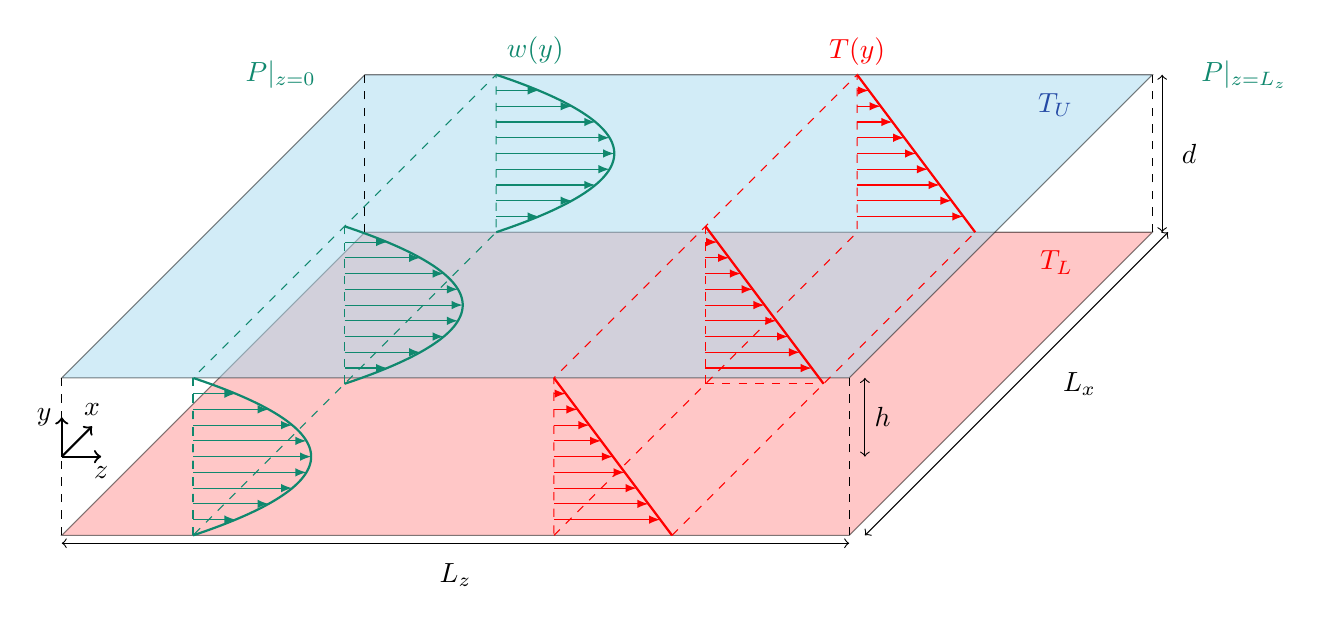
\begin{tikzpicture}
\def\H{1}
\def\W{10}
\def\L{10}

% Draw the bottom plate
\draw [fill=pink!75!red, opacity=0.5] (-\L/2,-\H,0) -- (\L/2,-\H,0) -- (\L/2, -\H, -\W) -- (-\L/2, -\H,-\W) -- cycle;

% Draw the top plate
\draw [fill=SkyBlue!75!white, opacity=0.5] (-\L/2,\H,0) -- (\L/2,\H,0) -- (\L/2, \H, -\W) -- (-\L/2,\H,-\W) -- cycle;

%  % Draw axes
\draw [dashed, thin] (-\L/2, -\H, 0) -- (-\L/2, \H, 0);
\draw [dashed, thin] (\L/2, -\H, 0) -- (\L/2, \H, 0);
\draw [dashed, thin] (\L/2, -\H, -\W) -- (\L/2, \H, -\W);
\draw [dashed, thin] (-\L/2, -\H, -\W) -- (-\L/2, \H, -\W);
%\draw [dashed, thin] (-1,0, 0) --++ (\L,0,0) --++ (0,0,-\W) --++ (-\L,0,0) -- cycle;
%  % \draw [thin, dashed] (-1,0) -- (6,0);

% Add dimensions
% L_x
\draw [<->] (-\L/2,-1.1*\H, 0) -- (\L/2,-1.1*\H,0);
\node[centered] at (0,-1.5*\H,0) {$L_z$};

% L_z
\draw [<->] (\L/2*1.025, -\H, -\W) -- (\L/2*1.025, \H,-\W);
\node[right] at (\L/2*1.05,0.0,-\W) {$d$};

% d
\draw [<->] (\L/2*1.04, -\H) -- (\L/2*1.04,-\H,-\W);
\node[centered] at (\L/2*1.2,-\H,-\W/2) {$L_x$};

% h
\draw [<->] (\L/2*1.04, 0, 0) -- (\L/2*1.04, \H, 0);
\node[right] at (\L/2*1.04,\H/2,0) {$h$};

% P
\node[left] at (-\L/2*1.1, \H, -\W) {\textcolor{PineGreen}{$P|_{z=0}$}};
\node[right] at (\L/2*1.1, \H, -\W) {\textcolor{PineGreen}{$P|_{z=L_z}$}};

% T
\node[left] at (\L/2*0.9, \H, -\W*0.9) {\textcolor{cyan!20!blue}{$T_U$}};
\node[left] at (\L/2*0.9, -\H, -\W*0.9) {\textcolor{red}{$T_L$}};

% Draw labels
\draw[->, thick] (-\L/2, 0, 0) -- (-\L/2,\H/2,0) node[left] {$y$};
\draw[->, thick] (-\L/2, 0, 0) -- (-\L/2+\H/2,0,0) node [below] {$z$};
\draw[->, thick] (-\L/2, 0, 0) -- (-\L/2,0,-\H) node[above] {$x$};

% Draw the velocity profile
\draw[PineGreen,thick,domain=-1:1,samples=200,smooth] plot ({(1-\x*\x)*1.5-\L/3}, \x) node[above right] {};
\draw[PineGreen,thick,domain=-1:1,samples=200,smooth] plot ({(1-\x*\x)*1.5-\L/3}, \x, -\W/2) node[above right] {};
\draw[PineGreen,thick,domain=-1:1,samples=200,smooth] plot ({(1-\x*\x)*1.5-\L/3}, \x, -\W) node[above right] {$w(y)$};
\draw[-,PineGreen,dashed] (-\L/3,-\H) -- (-\L/3,\H);
\draw[-,PineGreen,dashed] (-\L/3,-\H, -\W/2) -- (-\L/3,\H, -\W/2);
\draw[-,PineGreen,dashed] (-\L/3,-\H,0) -- (-\L/3,\H,0) -- (-\L/3,\H,-\W) -- (-\L/3,-\H,-\W) -- cycle;

\foreach \y in {-0.8,-0.6,...,0.8} {
    \draw[-latex,PineGreen] (-\L/3,\y, 0) -- ({(1-\y*\y)*1.5-\L/3},\y,0);
    \draw[-latex,PineGreen] (-\L/3,\y, -\W/2) -- ({(1-\y*\y)*1.5-\L/3},\y, -\W/2);
    \draw[-latex,PineGreen] (-\L/3,\y, -\W) -- ({(1-\y*\y)*1.5-\L/3},\y,-\W);
}

% Draw the temperature profile
\draw[red,thick,domain=-\H:\H,samples=200,smooth] plot ({(1/2*(1-\x)*1.5+\L/8)}, \x);
\draw[red,thick,domain=-\H:\H,samples=200,smooth] plot ({(1/2*(1-\x)*1.5+\L/8)}, \x, -\W/2);
\draw[red,thick,domain=-\H:\H,samples=200,smooth] plot ({(1/2*(1-\x)*1.5+\L/8)}, \x, -\W);
\draw[-,red,dashed] (\L/8,-\H,-\W/2) -- (\L/8,\H,-\W/2);
\draw[-,red,dashed] (\L/8,-\H,-\W/2) -- (\L/8 + 1.5,-\H,-\W/2);
\draw[-,red,dashed] (\L/8 +1.5,-\H,0) -- (\L/8 + 1.5,-\H,-\W);
\draw[-,red,dashed] (\L/8,-\H,0) -- (\L/8,-\H,-\W) -- (\L/8,\H, -\W) -- (\L/8,\H,0) -- cycle;
% % 
\foreach \y in {-0.8,-0.6,...,0.8} {
   \draw[-latex,red] (\L/8,\y) -- ({\L/8+(1/2*(1-\y)*1.5},\y);
   \draw[-latex,red] (\L/8,\y, -\W/2) -- ({\L/8+(1/2*(1-\y)*1.5},\y, -\W/2);
   \draw[-latex,red] (\L/8,\y, -\W) -- ({\L/8+(1/2*(1-\y)*1.5},\y, -\W);
}
% Add labels
\node[above,red] at (\L/8,1,-\W) {$T(y)$};
\end{tikzpicture}
\label{fig:rbpconfiguration}
\caption{The Rayleigh-B\'{e}nard Poiseuille (RBP) flow configuration.}
\end{figure}


The RBP configuration is illustrated in figure \ref{fig:rbpconfiguration}, where \DIFdelbegin \DIFdel{$z,y,x$ }\DIFdelend \DIFaddbegin \DIFadd{$z,x,y$ }\DIFaddend refer to spatial coordinates denoting the streamwise, spanwise and wall normal directions.
\DIFdelbegin \DIFdel{$L_z, L_x, d$ }\DIFdelend \DIFaddbegin \DIFadd{$L_z$, $L_x$, $d$, }\DIFaddend and $h$ \DIFdelbegin \DIFdel{corresponds }\DIFdelend \DIFaddbegin \DIFadd{correspond }\DIFaddend to the length, span, depth and half-height of the domain\DIFaddbegin \DIFadd{, }\DIFaddend respectively.
The RBP system is biperiodic along $z$ and $x$.
% We note that the asterisks$^*$, refer to variables in dimensional form.
The flow is driven by a pressure \DIFdelbegin \DIFdel{gradient }\DIFdelend \DIFaddbegin \DIFadd{difference }\DIFaddend along the streamwise $z$ direction, \DIFdelbegin \DIFdel{$\Delta P = P|_{z=0} - P|_{z=L_z} < 0$}\DIFdelend \DIFaddbegin \DIFadd{$\Delta P = P|_{z=L_z} - P|_{z=0} < 0$}\DIFaddend , leading to a laminar Poiseuille flow, $w(y) = W_c(1 - y^2)$, where $W_c$ is the laminar centerline velocity.
We consider a fully developed flow, where the boundary layer developing from the top and the bottom wall meets at the midplane $y=0$ and entrance effects are therefore neglected.
Like the RBC system, the RBP system is unstably stratified.
The temperature difference between the lower, $T_L$, and upper wall, $T_U$, is always positive, $\Delta T = T_L - T_U > 0$, leading to a stable linear conduction layer along the wall-normal direction, $T(y)$, if $\Delta T$ is kept sufficiently small.
The behaviour of RBP flows is \DIFdelbegin \DIFdel{govern }\DIFdelend \DIFaddbegin \DIFadd{governed }\DIFaddend by four dimensionless parameters\DIFdelbegin \DIFdel{,
}\DIFdelend \DIFaddbegin \DIFadd{:
}\DIFaddend \begin{equation}\label{eq:nondim_def}
    Re = W_c h / \nu, \quad Ra = \frac{\eta g d^3 \Delta T}{\nu \kappa}, \quad Pr = \DIFdelbegin \DIFdel{\frac{\kappa}{\nu}}\DIFdelend \DIFaddbegin \DIFadd{\frac{\nu}{\kappa}}\DIFaddend , \quad \Gamma = L/2d,
\end{equation}
where $Ra, Re, Pr, \Gamma$ \DIFdelbegin \DIFdel{refers to }\DIFdelend \DIFaddbegin \DIFadd{refer to the }\DIFaddend Reynolds, Rayleigh, Prandtl numbers and aspect ratio and $\eta, g, \nu, \kappa,$ are the thermal expansion coefficient, acceleration due to gravity, kinematic viscosity, \DIFaddbegin \DIFadd{and }\DIFaddend thermal diffusivity, respectively.
The Reynolds number, $Re$, and the Rayleigh number, $Ra$, are dimensionless parameters that characterise the relative influence of shear and buoyancy respectively.
For sufficiently large values of $Re$ and $Ra$, RBP flows may undergo a transition to shear-driven turbulence or \DIFdelbegin \DIFdel{convection-driven }\DIFdelend \DIFaddbegin \DIFadd{buoyancy-driven }\DIFaddend convection.
In the absence of shear, $Re = 0$, the RBP configuration reduces to the classical \DIFdelbegin \DIFdel{buoyancy driven }\DIFdelend \DIFaddbegin \DIFadd{buoyancy-driven }\DIFaddend Rayleigh-B\'{e}nard convection, which forms a bistable system between stationary and chaotic convection rolls slightly above the \DIFdelbegin \DIFdel{critial }\DIFdelend \DIFaddbegin \DIFadd{critical }\DIFaddend $Ra$.
The influence of $Re$ on bistability remains unexplored.

In the first part of this thesis, we focus on the transitional regime by investigating whether buoyancy forces promote the transition to shear-driven turbulence and \DIFdelbegin \DIFdel{examing }\DIFdelend \DIFaddbegin \DIFadd{examining }\DIFaddend the effect of shear on convection in large domains. 
The second part of this thesis \DIFdelbegin \DIFdel{explore }\DIFdelend \DIFaddbegin \DIFadd{explores }\DIFaddend the state space structure of a bistable system between a chaotic convection roll state and a stationary convection roll state (see spiral defect chaos and ideal straight rolls in \S \ref{sec:bkgrd_RBC}) of Rayleigh-B\'{e}nard convection.
%DIF <  In the limiting case without unstable stratification, $Ra = 0$, the system reduces to the wall-bounded plane Poiseuille flow (PPF), where the transition towards subscritical shear-driven turbulence may be expected for a sufficiently large pressure gradient.
%DIF <  For instance, do buoyancy forces promote the transition to shear-driven turbulence and how does shear influence the convection? 
%DIF <  To describe the motion of the fluid in RBP configurations, we consider the non-dimensionalised Navier-Stokes equations with Boussinessq approximations,
%DIF <  \begin{subequations}\label{eq:rbp_equations}
%DIF <  \begin{equation}
%DIF <      \frac{\partial \mathbf{u}}{\partial t} + (\mathbf{u}\cdot\nabla)\mathbf{u} = -\nabla p + \frac{1}{Re}\nabla^2 \mathbf{u} + \frac{Ra}{Re^2Pr} \theta,
%DIF <  \end{equation}
%DIF <  \begin{equation}
%DIF <      \frac{\partial \theta}{\partial t} + (\mathbf{u} \cdot \nabla)\theta = \frac{1}{RePr}\nabla^2 \theta,
%DIF <  \end{equation}
%DIF <  \begin{equation}
%DIF <      \nabla \cdot \mathbf{u} = 0.
%DIF <  \end{equation}
%DIF <  \end{subequations}
%DIF <  where $\mathbf{u}(\mathbf{x}), \theta(\mathbf{x}), p(\mathbf{x})$ refers to the nondimensionalised velocity, temperature and presure respectively.
%DIF <  The key control parameters for RBP flows are the Rayleigh number, $Ra$, Reynolds number, $Re$, Prandlt number $Pr$, which are defined as follows,
%DIF <  \begin{equation}
%DIF <      Ra = \eta g d^3 \Delta T / \nu \kappa, \quad Re = W_c h / \nu, \quad Pr = \kappa / \nu, \quad \Gamma = L/2d,
%DIF <  \end{equation}
%DIF <  where $\eta, g, \Delta T, \nu, \kappa, W_c, h, d, L$ are the thermal expansion coefficient, acceleration due to gravity, temperature difference between the bottom and top wall, kinematic viscosity, thermal diffusivity, laminar centreline velocity, domain's half-depth, full-depth, length or span respectively.

The structure of this introductory chapter is as follows:
\DIFdelbegin \DIFdel{we }\DIFdelend \DIFaddbegin \DIFadd{We }\DIFaddend begin our discussion on the development of hydrodynamic stability theory of wall-bounded shear flows in \S \ref{sec:bkgrd_transitional}.
Theoretical frameworks used in the study of the stability of fluid flow, including linear modal/non-modal stability, nonlinear dynamical systems and the spatio-temporal dynamics of transitional shear flows will be discussed.
Throughout \S \ref{sec:bkgrd_transitional}, we apply these concepts in the context of plane Poiseuille flows (PPF).
This \DIFaddbegin \DIFadd{is }\DIFaddend followed by the developments of Rayleigh-B\'{e}nard convection (RBC) in \S \ref{sec:bkgrd_RBC}.
Finally, we review the developments in RBP flows \S \ref{sec:bkgrd_RBP}, before concluding this chapter with \DIFaddbegin \DIFadd{the objectives of this thesis in \S \ref{sec:bkgrd_objs} and }\DIFaddend an outline of \DIFdelbegin \DIFdel{the thesis in \S \ref{sec:bkgrd_thesis_outline}}\DIFdelend \DIFaddbegin \DIFadd{its structure in \S \ref{sec:bkgrd_outline}}\DIFaddend .


% We first discuss the key developments of plane Poiseuille flow (PPF) outlining the key theoretical framework for analysing the stability of fluid flows. This is then followed by Rayleigh-B\'{e}nard convection (RBC) in \S \ref{sec:bkgrd_RBC}.

%%%%%%%%%%%%%%%%%%%%%%%%
% Plane Poiseuille Flows
%%%%%%%%%%%%%%%%%%%%%%%%

\section{Transitional wall-bounded shear flows}\label{sec:bkgrd_transitional}
Wall-bounded shear flows \DIFdelbegin \DIFdel{concerns }\DIFdelend \DIFaddbegin \DIFadd{concern }\DIFaddend the motion of the fluid flowing \DIFdelbegin \DIFdel{in }\DIFdelend parallel to walls, typically bounded by one or more walls.
\DIFdelbegin \DIFdel{Near }\DIFdelend \DIFaddbegin \DIFadd{At }\DIFaddend the wall, the fluid comes to rest due to the no-slip boundary condition, resulting in a velocity gradient perpendicular to the wall, giving rise to shear within the fluid, commonly known as \textit{wall-bounded shear flows}.
%DIF <  The fluid closest to the wall comes to a rest, satisfying the no-slip boundary condition in the presence of a wall.
%DIF <  As a consequence, a velocity gradient in the direction perpendicular from the wall develops, where the fluid layer becomes \emph{sheared} due to the pressence of the wall - referred to wall-bounded sheared flows.
%DIF <  In Newtonian fluids, shear stresses are directly proportionate to the velocity gradient by the fluids kinetic viscosity, $\nu$, given as,
%DIF <  \begin{equation}\label{eq:shear}
%DIF <     \tau = \nu \frac{\partial u}{\partial y},
%DIF <  \end{equation}
%DIF <  where $\tau$, $\nu$, and $\frac{\partial u}{\partial y}$ refers to shear stresses - hence wall-bounded shear flows.
Examples include the pressure-driven plane Poiseuille flow (channel flow), Hagen-Poiseuille flow (pipe flow), plane Couette flow and flat plate boundary layers.
These geometrically simple configurations \DIFdelbegin \DIFdel{provides }\DIFdelend \DIFaddbegin \DIFadd{provide }\DIFaddend a convenient framework amenable to the mathematical analysis of fluid motion \DIFdelbegin \DIFdel{subjected to }\DIFdelend \DIFaddbegin \DIFadd{under }\DIFaddend shear.
Depending on the degree of shear, the fluid motion can be either laminar, where the fluid layers move in smooth parallel \DIFdelbegin \DIFdel{'laminates'}\DIFdelend \DIFaddbegin \DIFadd{laminates}\DIFaddend , or turbulent, characterised by chaotic eddying motions.
We also note \DIFdelbegin \DIFdel{that there is }\DIFdelend a transitional regime \DIFdelbegin \DIFdel{where }\DIFdelend \DIFaddbegin \DIFadd{in which }\DIFaddend both states can coexist\DIFdelbegin \DIFdel{discuss later}\DIFdelend .
A central question is \DIFdelbegin \DIFdel{predicting }\DIFdelend \DIFaddbegin \DIFadd{the prediction of }\DIFaddend the transition from the laminar regime to \DIFdelbegin \DIFdel{the turbulence.
%DIF <  One of the central questions is on the prediction on the transition to turbulence, specifically, when is turbulence expected as shear is increased?
%DIF <  plane Poiseuille flow (PPF) describes the motion of a fluid confined between two infinitely extended parallel walls, driven by a pressure gradient, also referred to as channel flow.
%DIF <  It belongs to a general class of wall-bounded shear flows, consisting of plane Couette flow, pipe (Hagen-Poiseuille) flow and flat plate boundary layer flow.
}\DIFdelend \DIFaddbegin \DIFadd{turbulence.
}\DIFaddend 

The first investigation into this transition was conducted by \DIFdelbegin \DIFdel{\mbox{%DIFAUXCMD
\cite{reynolds_xxix_1883}}\hspace{0pt}%DIFAUXCMD
.
%DIF <  The earliest investigation into this transition dates back to the pipe flow experiments of \cite{reynolds_xxix_1883}.
}\DIFdelend \DIFaddbegin \DIFadd{\mbox{%DIFAUXCMD
\citet{reynolds_xxix_1883}}\hspace{0pt}%DIFAUXCMD
.
%DIF >  The earliest investigation into this transition dates back to the pipe flow experiments of \citet{reynolds_xxix_1883}.
}\DIFaddend In his experimental setup, \DIFaddbegin \DIFadd{Reynolds controlled }\DIFaddend the flow speed through the pipe \DIFdelbegin \DIFdel{could be controlled }\DIFdelend by regulating the inlet pressure, \DIFdelbegin \DIFdel{while injecting }\DIFdelend \DIFaddbegin \DIFadd{and injected }\DIFaddend dye to visualise the flow, as illustrated in figure \ref{fig:reynolds}(a).
At low speeds, the fluid \DIFdelbegin \DIFdel{remained }\DIFdelend \DIFaddbegin \DIFadd{is }\DIFaddend laminar, resulting \DIFdelbegin \DIFdel{to }\DIFdelend \DIFaddbegin \DIFadd{in }\DIFaddend a single streak of steady dye \DIFaddbegin \DIFadd{shown }\DIFaddend in figure \ref{fig:reynolds}(b).
As the speed \DIFaddbegin \DIFadd{is }\DIFaddend increased, the dye \DIFdelbegin \DIFdel{begin }\DIFdelend \DIFaddbegin \DIFadd{began }\DIFaddend to exhibit irregular `sinuous' motions interspersed with laminar regions shown in figure \ref{fig:reynolds}(c).
This is now referred to as the transitional regime, \DIFdelbegin \DIFdel{alternating between the }\DIFdelend \DIFaddbegin \DIFadd{which alternates between }\DIFaddend laminar and turbulent states.
Beyond a critical speed, the dye breaks down entirely into chaotic \DIFdelbegin \DIFdel{`eddies'}\DIFdelend \DIFaddbegin \DIFadd{eddies}\DIFaddend , mixing with the surrounding fluid and discolouring the flow with dye downstream\DIFaddbegin \DIFadd{, shown }\DIFaddend in figure \ref{fig:reynolds}(d).
This regime is now identified as turbulence.

Reynolds proposed that the threshold between the laminar, transitional and turbulent regimes could be characterised by a non-dimensional parameter, now referred to as the Reynolds number,
\begin{equation}
    Re = U D/\nu,
\end{equation}
where $U$ is the centerline velocity in the pipe, $D$, the pipe diameter and $\nu$, the kinematic viscosity.
He observed that flow through the pipe remained \textit{stable} and laminar for $Re < 1900$, while it became \textit{unstable} and turbulent for $Re > 2000$ \citep{reynolds_iv_1895}, introducing the notion of flow \textit{stability}.
\begin{figure}[h]
    \centering
    \includegraphics[width=1\textwidth]{Background/Figures/Reynolds.pdf}
    \caption{(a) Osbourne Reynolds pipe experiment with the dye injection apparatus, illustrating the (b) laminar flow, (c) transitional regime and (d) turbulent flow as the flow speed is increased, taken from \protect\DIFdelbeginFL \DIFdelFL{\mbox{%DIFAUXCMD
\cite{reynolds_xxix_1883}}\hspace{0pt}%DIFAUXCMD
}\DIFdelendFL \DIFaddbeginFL \DIFaddFL{\mbox{%DIFAUXCMD
\citet{reynolds_xxix_1883}}\hspace{0pt}%DIFAUXCMD
}\DIFaddendFL .}
    \label{fig:reynolds}
\end{figure}

%%%%%%%%%%%%%%%%%%%%%%%%%%%
% Linear Stability Analysis
%%%%%%%%%%%%%%%%%%%%%%%%%%%

\subsection{Linear Stability Analysis}
Following \DIFdelbegin \DIFdel{Reynolds' }\DIFdelend \DIFaddbegin \DIFadd{the }\DIFaddend experiment, interest towards the mathematical analysis of the stability of laminar flows grew in \DIFdelbegin \DIFdel{early $20^{st}$ }\DIFdelend \DIFaddbegin \DIFadd{the early $20^{th}$ }\DIFaddend century.
The mathematical approach typically begins by decomposing the velocity field, $\mathbf{u}(\mathbf{x},t)$, into a laminar (base) state, \DIFdelbegin \DIFdel{$U(y)$}\DIFdelend \DIFaddbegin \DIFadd{$\mathbf{U}(\mathbf{x}) = U(y)\mathbf{e_x}$}\DIFaddend , and the velocity perturbations, $\mathbf{u}'(\mathbf{x},t)$, with pressure similarly decomposed as
\DIFdelbegin \DIFdel{,
}\DIFdelend \begin{equation}
\mathbf{u}(\mathbf{x}) = \DIFdelbegin \DIFdel{U}\DIFdelend \DIFaddbegin \DIFadd{\mathbf{U}}\DIFaddend (\DIFdelbegin \DIFdel{y}\DIFdelend \DIFaddbegin \DIFadd{\mathbf{x}}\DIFaddend ) + \mathbf{u}'(\mathbf{x},t), \quad \text{and} \quad p(\mathbf{x},t) = P(x) + p'(\mathbf{x},t).
\end{equation}
Substituting \DIFaddbegin \DIFadd{the decomposition }\DIFaddend into the Navier-Stokes equations and linearising (neglecting nonlinear terms), we get
\DIFdelbegin \DIFdel{,
%DIF <  Next, we the substitute the formulations for the decomposed velocity and pressure into the Navier-Stokes equations of equation \eqref{eq:rbp_equations} and drop the nonlinear pertubrations terms $(\mathbf{u'}\cdot \nabla)\mathbf{u'}$,
}\DIFdelend \begin{subequations}\label{eq:shear_linearised}
\begin{equation}
    \frac{\partial \mathbf{u'}}{\partial t} + (\DIFdelbegin \DIFdel{U }\DIFdelend \DIFaddbegin \DIFadd{\mathbf{U} }\DIFaddend \cdot\nabla)\mathbf{u'} + (\mathbf{u'}\cdot\nabla)\DIFdelbegin \DIFdel{U}\DIFdelend \DIFaddbegin \DIFadd{\mathbf{U} }\DIFaddend = -\nabla p' + \frac{1}{Re}\nabla^2 \mathbf{u'},
\end{equation}
\begin{equation}
    \nabla \cdot \mathbf{u}' = 0,
\end{equation}
\end{subequations}
known as the linearised Navier-Stokes equations. 
This \DIFaddbegin \DIFadd{is }\DIFaddend commonly followed by introducing a wavelike ansatz (mode) for the perturbations, and analysed by considering their behaviour independently, referred to as modal analysis in \S \ref{subsec:modal}, or their coupled dynamics, referred to as non-modal analysis in \S \ref{subsec:nonmodal}.

%DIF <  In general two ways to analysis the linearised Navier-Stokes equations by considering the behaviour of each mode independently in \S \ref{subsec:modal} and their coupled dynamics in \S \ref{subsec:nonmodal}
\DIFdelbegin %DIFDELCMD < 

%DIFDELCMD < %%%
\DIFdelend %%%%%%%%%%%%%%%%%
% MODAL STABILITy
%%%%%%%%%%%%%%%%%

\subsubsection{Modal analysis}\label{subsec:modal}
It is \DIFdelbegin \DIFdel{covenient }\DIFdelend \DIFaddbegin \DIFadd{convenient }\DIFaddend to eliminate the pressure \DIFdelbegin \DIFdel{terms }\DIFdelend \DIFaddbegin \DIFadd{term }\DIFaddend by reformulating equation \eqref{eq:shear_linearised} using the wall-normal perturbation velocity, $v'$, and wall-normal vorticity, $\eta' = \partial u'/ \partial z - \partial w' / \partial x$, variables.
Using $(v, \eta)$, we introduce a modal ansatz\DIFdelbegin \DIFdel{for them,
}\DIFdelend \DIFaddbegin \DIFadd{:
}\DIFaddend \begin{equation}\label{eq:shear_ansatz}
    v'(\mathbf{x},t ) = \tilde{v}(y)e^{i(\alpha x + \beta z - \omega t)} \DIFaddbegin \DIFadd{+ \text{c.c}}\DIFaddend , \quad \text{and} \quad \eta'(\mathbf{x}, t) = \tilde{\eta}(y)e^{i(\alpha x + \beta z - \omega t)} \DIFdelbegin \DIFdel{.
}\DIFdelend \DIFaddbegin \DIFadd{+ \text{c.c},
}\DIFaddend \end{equation}
where $\alpha, \beta, \omega$ \DIFdelbegin \DIFdel{denotes }\DIFdelend \DIFaddbegin \DIFadd{and c.c denote }\DIFaddend the streamwise and spanwise wavenumbers, \DIFdelbegin \DIFdel{and }\DIFdelend complex frequency (i.e. $\omega = \omega_r + i\omega_i$) \DIFaddbegin \DIFadd{and complex conjugate}\DIFaddend , respectively.
Substituting this ansatz into \DIFdelbegin \DIFdel{linearised equations lead }\DIFdelend \DIFaddbegin \DIFadd{the linearised equations leads }\DIFaddend to the classical Orr-Sommerfeld and Squire equations \citep{orr_stability_1907,sommerfeld_beitrag_1909,squire_stability_1933, schmid_stability_2001},
%DIF <  \begin{equation}
%DIF <      \mathbf{L}\mathbf{\tilde{q}} = i\omega\mathbf{M}\mathbf{\tilde{q}}
%DIF <  \end{equation}
\begin{subequations}
\begin{equation}\label{eq:OSQ}
    \begin{pmatrix}
        \mathcal{L}_{OS} & 0 \\
        i\beta U' & \mathcal{L}_{SQ}
    \end{pmatrix}
    \begin{pmatrix}
        \tilde{v} \\
        \tilde{\eta}
    \end{pmatrix}
    = 
    i\omega
    \begin{pmatrix}
        k^2 - \mathcal{D}^2 & 0 \\
        0 & 1 
    \end{pmatrix}
    \begin{pmatrix}
        \tilde{v} \\
        \tilde{\eta}
    \end{pmatrix}\DIFdelbegin \DIFdel{.
}\DIFdelend \DIFaddbegin \DIFadd{,
}\DIFaddend \end{equation}
%DIF <  \begin{equation}\label{eq:OSQ}
%DIF <      \left[
%DIF <      -i\omega 
%DIF <      \begin{pmatrix}
%DIF <          k^2 - \mathcal{D}^2 & 0 \\
%DIF <          0 & 1 
%DIF <      \end{pmatrix}
%DIF <      + 
%DIF <      \begin{pmatrix}
%DIF <          \mathcal{L}_{OS} & 0 \\
%DIF <          i\beta U' & \mathcal{L}_{SQ} 
%DIF <      \end{pmatrix}
%DIF <  \right ]
%DIF <      \begin{pmatrix}
%DIF <          \tilde{v} \\
%DIF <          \tilde{\eta}
%DIF <      \end{pmatrix}
%DIF <      = \mathbf{0},
%DIF <  \end{equation}
\DIFdelbegin \DIFdel{\text{with}
  }\DIFdelend \DIFaddbegin \DIFadd{\text{with}
  }\DIFaddend \begin{equation} 
      \mathcal{L}_{OS} = i\alpha U(k^2-\mathcal{D}^2) + i\alpha U'' + \frac{1}{Re}(k^2 - \mathcal{D}^2)^2,
      \quad \mathcal{L}_{SQ} = i\alpha U + \frac{1}{Re}(k^2 - \mathcal{D}^2)\DIFdelbegin \DIFdel{.
  }\DIFdelend \DIFaddbegin \DIFadd{,
  }\DIFaddend \end{equation}
\end{subequations}
where $\mathcal{D} = d/dy, k^2 = \alpha^2 + \beta^2$ and $U''$ is the second derivative of $U(y)$.
% $k^2, \mathcal{D}, U', U''$ denotes the sum of squared wavenumbers, $k^2 = \alpha^2 + \beta^2$, differential operator in $y$, first- and second- derivative of the laminar velocity, respectively.
Equation \eqref{eq:OSQ} is \DIFdelbegin \DIFdel{an }\DIFdelend \DIFaddbegin \DIFadd{a }\DIFaddend generalised eigenvalue problem with eigenvalue $i\omega$, which determines the growth of perturbations.

The goal of modal stability analysis is to determine the critical Reynolds number $Re_c$, defined as the lowest value of $Re$, for all $\alpha$ and $\beta$ in which $\Im[\omega] = 0$.
For $Re > Re_c$, perturbations can grow exponentially, indicating instability.
% For $Re > Re_c$, perturbations could grow exponentially, departing from the laminar state.
% In other words, we consider the behaviour of each $\alpha-\beta$ mode independently, herein referred to as \emph{modal} analysis.
Squire's theorem states that for every unstable three-dimensional perturbation,  there \DIFdelbegin \DIFdel{exist }\DIFdelend \DIFaddbegin \DIFadd{exists }\DIFaddend an unstable two-dimensional perturbation, with a lower $Re_c$ \citep{squire_stability_1933}.
This implies that the most linearly unstable perturbation of wall-bounded flows is \DIFdelbegin \DIFdel{two dimensional}\DIFdelend \DIFaddbegin \DIFadd{two-dimensional}\DIFaddend .
Calculations by \DIFdelbegin \DIFdel{\mbox{%DIFAUXCMD
\cite{tollmien_uber_1928} }\hspace{0pt}%DIFAUXCMD
and \mbox{%DIFAUXCMD
\cite{schlichting_zur_1933} }\hspace{0pt}%DIFAUXCMD
}\DIFdelend \DIFaddbegin \DIFadd{\mbox{%DIFAUXCMD
\citet{tollmien_uber_1928} }\hspace{0pt}%DIFAUXCMD
and \mbox{%DIFAUXCMD
\citet{schlichting_zur_1933} }\hspace{0pt}%DIFAUXCMD
}\DIFaddend for a flat-plate boundary layer flow yielded a critical Reynolds number based on displacement thickness, $\delta^*$, of $Re_{ind} = U_\infty \delta^* / \nu = 520$ \footnote{In \DIFdelbegin \DIFdel{the literature of }\DIFdelend stability theory, $Re_{ind}$ refers to the indifference Reynolds number which is \DIFdelbegin \DIFdel{similar }\DIFdelend \DIFaddbegin \DIFadd{related }\DIFaddend to\DIFaddbegin \DIFadd{, but distinct from, }\DIFaddend the critical Reynolds number, $Re_{c}$ \DIFaddbegin \DIFadd{\mbox{%DIFAUXCMD
\citep{schlichting_onset_2017}}\hspace{0pt}%DIFAUXCMD
}\DIFaddend . \DIFdelbegin \DIFdel{However, }\DIFdelend \DIFaddbegin \DIFadd{Because }\DIFaddend boundary layer transition \DIFdelbegin \DIFdel{often takes place }\DIFdelend \DIFaddbegin \DIFadd{occurs }\DIFaddend over a finite distance, \DIFdelbegin \DIFdel{and }\DIFdelend the indifference point is \DIFdelbegin \DIFdel{used }\DIFdelend \DIFaddbegin \DIFadd{introduced }\DIFaddend to \DIFdelbegin \DIFdel{disambiguate }\DIFdelend \DIFaddbegin \DIFadd{distinguish }\DIFaddend between the onset of transition and the \DIFdelbegin \DIFdel{critical }\DIFdelend point \DIFdelbegin \DIFdel{of completed transition}\DIFdelend \DIFaddbegin \DIFadd{at which the flow becomes fully turbulent}\DIFaddend .\DIFdelbegin %DIFDELCMD < \MBLOCKRIGHTBRACE%%%
\DIFdel{\mbox{%DIFAUXCMD
\citep{schlichting_onset_2017}}\hspace{0pt}%DIFAUXCMD
.
These two dimensional }\DIFdelend \DIFaddbegin }
\DIFadd{These two-dimensional }\DIFaddend unstable eigenmodes are known as Tollmien-Schlichting (T.S) waves.
%DIF <  In their honour, the unstable two-dimensional perturbations of the Orr-Sommerfeld operator is referred to as Tollmien-Schlicting (T.S) waves.
In plane Poiseuille flow, the critical Reynolds number is $Re_{c} = 5772.2$ with a critical wavenumber of $\alpha_c = 1.02$ \citep{orszag_accurate_1971}.
However, experiments reveal that transition to turbulence can occur at a lower Reynolds number, around \DIFdelbegin \DIFdel{, }\DIFdelend $Re \sim 1000 - 2000$ \citep{davies_experimental_1928, patel_observations_1969,dean_reynolds_1978,iida_relaminarization_1998,tsukahara_dns_2014}, highlighting a key limitation of modal analysis.
Similar discrepancies are observed in plane Couette and pipe flows \citep{meseguer_linearized_2003}, where the laminar state is linearly stable for all $Re$, yet transition to turbulence occurs.
Despite these limitations, modal analysis predicts instabilities in other systems such as Rayleigh-B\'{e}nard convection and Taylor-Couette flow \citep{chandrasekhar_stability_1968}.
Further extensions of modal stability, including spatial instability analysis \citep{huerre_local_1990}, and secondary instability \citep{orszag_secondary_1983} are well established and are beyond the scope of this thesis.
%DIF <  Likewise, the onset of turbulence appear near $Re_{x,c} \approx 5 \times 10^5$ for flat plat boundary layer.
%DIF <  The aim of linear stability analysis it to search for eigenvalues across $\alpha, \beta, Re$, such that $w_i \geq 0$, denoting an exponential growth of perturbations above a critical Reynolds number defined as $Re_c= \min(\alpha, \beta, Re)|_{\omega = 0}$.
%DIF <  Interestingly, linear stability analysis for pipe flow predicts a stable laminar flow for all Reynolds numbers \citep{romanov_stability_1973}, contradicting experiments \citep{reynolds_xxix_1883,avila_onset_2011}.
%DIF <  A similar result holds for the plane Couette flow \citep{meseguer_linearized_2003}.
%DIF <  The critical Reynolds number for the onset of unstable infinitesimal perturbutations in plane Poiseuille flow (PPF) occurs at $Re_{c} = 5772.2$ \citep{orszag_accurate_1971}.
%DIF <  Despite its limitation, linear analysis analysis succeeds in predicting the critical Rayleigh number in Rayleigh-B\'{e}nard convection.
%DIF <  Despite it failures, it has succeeded in other configurations, such as Rayleigh-B\'{e}nard convection, and Taylor-Couette flow \citep{bodenschatz_recent_2000}, predicting the onset of convection and Taylor rolls are the correct critical parameters.

%%%%%%%%%%%%%%%%%%%%%
% Non-modal stability
%%%%%%%%%%%%%%%%%%%%%
\DIFdelbegin %DIFDELCMD < 

%DIFDELCMD < %%%
\DIFdelend \subsubsection{Non-modal stability}\label{subsec:nonmodal}
One of \DIFdelbegin \DIFdel{a }\DIFdelend \DIFaddbegin \DIFadd{the }\DIFaddend major limitations of modal analysis is that it treats each eigenmode independently.
However, the interaction between decaying eigenmodes can lead to \DIFdelbegin \DIFdel{a }\DIFdelend transient growth, \DIFdelbegin \DIFdel{where }\DIFdelend \DIFaddbegin \DIFadd{in which }\DIFaddend perturbations amplify temporarily before decaying asymptotically.
%DIF <  The method of analysis is referred to as \emph{non-modal} analysis, related to the normality of the linear Orr-Sommerfeld operator \citep{schmid_nonmodal_2007}.
\begin{figure}[h]
    \centering
    \includegraphics[width=\textwidth]{Background/Figures/PhasePotrait.pdf}
    \caption{(a) The phase portrait of the toy model with $Re = 15$, where red lines are phase lines of the toy model. The blue trajectory \DIFdelbeginFL \DIFdelFL{lead }\DIFdelendFL \DIFaddbeginFL \DIFaddFL{leads }\DIFaddendFL to transient growth and the green trajectory \DIFdelbeginFL \DIFdelFL{do }\DIFdelendFL \DIFaddbeginFL \DIFaddFL{does }\DIFaddendFL not (b) Time history of blue and green \DIFdelbeginFL \DIFdelFL{trajectory}\DIFdelendFL \DIFaddbeginFL \DIFaddFL{trajectories}\DIFaddendFL .}
    \label{fig:toy_model}
\end{figure}
To demonstrate an example of transient growth, we consider a two-dimensional toy model governing the time-evolution of $\mathbf{q} = (v, \eta)^T$ \DIFdelbegin \DIFdel{,
}\DIFdelend \DIFaddbegin \DIFadd{as 
}\DIFaddend \begin{equation}
    \frac{\mathrm{d}}{\mathrm{d}t} \begin{pmatrix} v \\ \eta \end{pmatrix}  = \begin{pmatrix} -\frac{1}{Re} & -1 \\ 0 & -\frac{2}{Re} \end{pmatrix} \begin{pmatrix} v \\ \eta \end{pmatrix},
\end{equation}
where $Re$ refers to the Reynolds number.
The toy model has negative eigenvalues, $(\lambda_1, \lambda_2) = (-1/Re, -2/Re)$, indicating \DIFdelbegin \DIFdel{asymptotic decay .
%DIF <  and unit eigenvectors $\mathbf{x_1} = (1, 0)$, $\mathbf{x_2} = \frac{1}{\sqrt{Re^2 + 1}}(Re, 1)$.
%DIF <  Judging from the negative eigenvalues, we conclude that $\mathbf{q}(t)$ will decay exponentially.
%DIF <  As $Re \rightarrow \infty$, the eigenvectors,  becoming increasingly aligned (non-orthogonal) leading to significant transient growth.
}\DIFdelend \DIFaddbegin \DIFadd{a linearly stable system where perturbations decay asymptotically.
}\DIFaddend At $Re = 15$, the eigenvectors, $\mathbf{x_1} = (1,0)$, $\mathbf{x}_2 = (1,\frac{1}{\sqrt{Re^2 + 1}})$, are highly non-orthogonal, becoming almost parallel\DIFaddbegin \DIFadd{, as }\DIFaddend shown in figure \ref{fig:toy_model}(a).
Notably, they become \DIFdelbegin \DIFdel{increasingly }\DIFdelend \DIFaddbegin \DIFadd{more }\DIFaddend linearly dependent as $Re \rightarrow \infty$.
For a particular initial condition, the energy\DIFdelbegin \DIFdel{$||q||^2 = \sqrt{v^2 + \eta^2}$}\DIFdelend \DIFaddbegin \DIFadd{, $||\mathbf{q}||_2 = \sqrt{v^2 + \eta^2}$}\DIFaddend , is amplified \DIFaddbegin \DIFadd{approximately }\DIFaddend four times before decaying\DIFdelbegin \DIFdel{in blue trajectory , shown in Figure }\DIFdelend \DIFaddbegin \DIFadd{, represented by the blue trajectory shown in figure }\DIFaddend \ref{fig:toy_model}(b).
Yet for another choice of initial condition, the trajectory decays asymptotically\DIFdelbegin \DIFdel{as }\DIFdelend \DIFaddbegin \DIFadd{, as indicated by }\DIFaddend the green trajectory\DIFdelbegin \DIFdel{indicates.
Despite }\DIFdelend \DIFaddbegin \DIFadd{.
Despite the presence of }\DIFaddend decaying eigenmodes, the toy model highlights the \DIFdelbegin \DIFdel{significance }\DIFdelend \DIFaddbegin \DIFadd{importance }\DIFaddend of transient growth, which depends on the choice of initial \DIFdelbegin \DIFdel{condition.
%DIF <  For a randomly selected initial condition with an energy-norm of $||\mathbf{q}_0||_2 = 15$, where $|| \cdot ||_2$ refers to the L2-norm, the trajectory in green decays exponentially for $t \in [0, 100]$ in figure \ref{fig:toy_model}(b).
%DIF <  In constrast, for a specifically chosen initial condition in shown as the blue trajectory, $||\mathbf{q}||_2$ is amplified nearly four times before decaying exponentially.
}\DIFdelend \DIFaddbegin \DIFadd{conditions.
}\DIFaddend 

The aim of non-modal stability analysis is to search for optimal initial conditions, $\mathbf{\tilde{q}}_0$, that \DIFdelbegin \DIFdel{leads }\DIFdelend \DIFaddbegin \DIFadd{lead }\DIFaddend to the maximum amplification, $G(\tau)$, over a time horizon $\tau$. 
This is posed as an \DIFdelbegin \DIFdel{optimistaion problem,
}\DIFdelend \DIFaddbegin \DIFadd{optimisation problem:
}\DIFaddend \begin{equation}\label{eq:transient_growth}
    %DIF <  G(t) = \max_{\mathbf{\tilde{q}}_0 \neq 0 } \frac{||\mathbf{\tilde{q}}(t)||^2}{||\mathbf{\tilde{q}}_0||^2}, \quad \text{s.t} \quad ||\mathbf{\tilde{q}}_0||^2 = 1,
    G(\tau) = \max_{\mathbf{\tilde{q}}_0 \neq 0 } \frac{\langle \mathbf{\tilde{q}}(\tau), \mathbf{\tilde{q}}(\tau) \rangle }{\langle \mathbf{\tilde{q}}_0, \mathbf{\tilde{q}}_0 \rangle }, \quad \text{s.t} \quad \langle \mathbf{\tilde{q}}_0, \mathbf{\tilde{q}}_0 \rangle = 1,
\end{equation}
where, $\langle \cdot, \cdot \rangle$ denotes the inner-product,
\begin{equation}
    \langle \mathbf{\tilde{q}}, \mathbf{\tilde{q}} \rangle = \int_\Omega \mathbf{\tilde{q}}^H \mathbf{\tilde{q}} \; \mathrm{d}\Omega,
\end{equation}
and $\mathbf{\tilde{q}}^ H$ refers to the complex conjugate transpose of $\mathbf{\tilde{q}}$.
By considering the linearised operator of \eqref{eq:OSQ}, we define a linear operator as \DIFdelbegin \DIFdel{,
}\DIFdelend \DIFaddbegin \DIFadd{follows:
}\DIFaddend \begin{equation}\label{eq:linear_evolution}
    \mathbf{\tilde{q}}(\tau) = \mathcal{A}(\tau) \mathbf{\tilde{q}}_0,
\end{equation}
which takes the solution from initial conditions, $\mathbf{\tilde{q}}_0$, to $\mathbf{\tilde{q}}(\tau)$ at time $\tau$.
\DIFdelbegin \DIFdel{Subtituting }\DIFdelend \DIFaddbegin \DIFadd{Substituting }\DIFaddend the expression above into equation \eqref{eq:transient_growth},
\begin{equation}\label{eq:transient_growth_adj}
    G(\tau) = \max_{\mathbf{\tilde{q}}_0 \neq 0 } \frac{\langle \mathcal{A}(\tau)\mathbf{\tilde{q}}_0, \mathcal{A}(\tau)\mathbf{\tilde{q}}_0 \rangle }{\langle \mathbf{\tilde{q}}_0, \mathbf{\tilde{q}}_0 \rangle} = \langle \mathbf{\tilde{q}}_0, \mathcal{A}^\dagger(\tau) \mathcal{A}(\tau)\mathbf{\tilde{q}}_0  \rangle \DIFaddbegin \footnote{\DIFadd{The adjoint, $\mathcal{A}^\dagger$, of operator, $\mathcal{A}$, statisfies the mathematical property of $\langle \mathcal{A} \mathbf{x}, \mathbf{y} \rangle = \langle \mathbf{x}, \mathcal{A}^\dagger\mathbf{y} \rangle$. By substituting $\mathcal{A}\mathbf{\tilde{q}_0}$ as $\mathcal{A}\mathbf{x}$, and $\mathcal{A}\mathbf{\tilde{q}_0}$ as $\mathbf{y}$, we arrive at $\langle \mathcal{A}(\tau)\mathbf{\tilde{q}_0}, \mathcal{A}(\tau)\mathbf{\tilde{q}_0} \rangle = \langle \mathbf{\tilde{q}_0}, \mathcal{A}(\tau)^\dagger \mathcal{A}(\tau)\mathbf{\tilde{q}_0}\rangle$.}} \DIFaddend = \lambda_{max} (\mathcal{A}\DIFaddbegin \DIFadd{^\dagger}\DIFaddend (\tau) \DIFdelbegin \DIFdel{^\dagger }\DIFdelend \mathcal{A}(\tau)),
\end{equation}
where \DIFdelbegin \DIFdel{$\mathcal{A}^\dagger$ refers to }\DIFdelend \DIFaddbegin \DIFadd{$\mathcal{A}^\dagger(\tau)$ is }\DIFaddend the adjoint of \DIFdelbegin \DIFdel{$\mathcal{A}(t)$}\DIFdelend \DIFaddbegin \DIFadd{$\mathcal{A}(\tau)$}\DIFaddend .
The maximum amplification factor\DIFdelbegin \DIFdel{$\max G(t)$ }\DIFdelend \DIFaddbegin \DIFadd{, $G(\tau)$, }\DIFaddend is the largest eigenvalue of $\mathcal{A}^\dagger(\tau)\mathcal{A}(\tau)$ \DIFaddbegin \DIFadd{and the corresponding eigenvector, $\mathbf{\tilde{q}}_0$, denotes the eigenvector}\DIFaddend .
The eigenvalue problem is given as
\DIFdelbegin \DIFdel{,
}\DIFdelend \begin{equation}
    \mathcal{A}^\dagger(\DIFdelbegin \DIFdel{t}\DIFdelend \DIFaddbegin \DIFadd{\tau}\DIFaddend )\mathcal{A}(\DIFdelbegin \DIFdel{t}\DIFdelend \DIFaddbegin \DIFadd{\tau}\DIFaddend ) \mathbf{\tilde{q}}_0 = \lambda \mathbf{\tilde{q}}_0\DIFdelbegin \DIFdel{,
}\DIFdelend \DIFaddbegin \DIFadd{.
}\DIFaddend \end{equation}
\DIFdelbegin \DIFdel{where $\mathbf{\tilde{q}}_0$ refers to the eigenvector denoting the optimal initial condition.
}\DIFdelend %DIF >  where $\mathbf{\tilde{q}}_0$ refers to the eigenvector denoting the optimal initial condition.
For a detailed derivation of the optimal initial conditions or forcing, the reader is referred to \DIFdelbegin \DIFdel{\mbox{%DIFAUXCMD
\cite{butler_three-dimensional_1992} }\hspace{0pt}%DIFAUXCMD
and \mbox{%DIFAUXCMD
\cite{schmid_nonmodal_2007}}\hspace{0pt}%DIFAUXCMD
}\DIFdelend \DIFaddbegin \DIFadd{\mbox{%DIFAUXCMD
\citet{butler_three-dimensional_1992} }\hspace{0pt}%DIFAUXCMD
and \mbox{%DIFAUXCMD
\citet{schmid_nonmodal_2007}}\hspace{0pt}%DIFAUXCMD
}\DIFaddend .
An alternative method \DIFdelbegin \DIFdel{of }\DIFdelend \DIFaddbegin \DIFadd{for }\DIFaddend computing the optimal transient growth is \DIFdelbegin \DIFdel{by analysing the pseudospectral of }\DIFdelend \DIFaddbegin \DIFadd{to analyse the pseudospectra of the }\DIFaddend linear operators discussed \DIFdelbegin \DIFdel{by \mbox{%DIFAUXCMD
\cite{trefethen_pseudospectra_1997}}\hspace{0pt}%DIFAUXCMD
}\DIFdelend \DIFaddbegin \DIFadd{in \mbox{%DIFAUXCMD
\citet{trefethen_pseudospectra_1997}}\hspace{0pt}%DIFAUXCMD
}\DIFaddend .

Both \DIFdelbegin \DIFdel{two-, and }\DIFdelend \DIFaddbegin \DIFadd{two-and }\DIFaddend three-dimensional non-modal \DIFdelbegin \DIFdel{anlyses }\DIFdelend \DIFaddbegin \DIFadd{analyses }\DIFaddend reveal mechanisms for transient growth.
In two-dimensions, the optimal initial conditions are in the form of \DIFdelbegin \DIFdel{near wall vorticies }\DIFdelend \DIFaddbegin \DIFadd{near-wall vortices }\DIFaddend tilted upstream, which amplifies transiently via the Orr-mechanism \citep{orr_stability_1907, farrell_optimal_1988,reddy_pseudospectra_1993}.
In three-dimensions, streamwise vortices are optimal, leading to the \DIFdelbegin \DIFdel{the }\DIFdelend amplification of streamwise streaks via the \DIFdelbegin \DIFdel{well known }\DIFdelend \DIFaddbegin \DIFadd{well-known }\DIFaddend lift-up effect \citep{ellingsen_stability_1975,reddy_energy_1993}.
Notably, the spacing of these streaks analysed using non-modal analysis at higher Reynolds number has been consistently reported to occur around 100 wall units \citep{del_alamo_linear_2006,pujals_note_2009,hwang_linear_2010}, which supports experimental observations of streak spacing in turbulent boundary layers \citep{kline_structure_1967, smith_characteristics_1983}.

The main \DIFdelbegin \DIFdel{results from }\DIFdelend \DIFaddbegin \DIFadd{result of the }\DIFaddend non-modal analysis is that \DIFdelbegin \DIFdel{three dimensional }\DIFdelend \DIFaddbegin \DIFadd{three-dimensional }\DIFaddend perturbations can lead to strong transient growth at subcritical Reynolds numbers, contradicting the \DIFdelbegin \DIFdel{two dimensional TS waves from }\DIFdelend \DIFaddbegin \DIFadd{two-dimensional TS waves predicted by }\DIFaddend modal analysis.
Both modal and non-modal mechanisms \DIFdelbegin \DIFdel{highlight }\DIFdelend \DIFaddbegin \DIFadd{provide }\DIFaddend important insights into the linear mechanisms \DIFdelbegin \DIFdel{which might }\DIFdelend \DIFaddbegin \DIFadd{that may }\DIFaddend be responsible for the transition from laminar to turbulent \DIFdelbegin \DIFdel{flows.
%DIF <  Contrary to linear stability analysis which confers two-dimensional perturbations as linearly unstable, the key result in this analysis is that three-dimensional initial conditions, $\alpha = 0$, confer the optimal initial conditions leading to large transient growth at subcritical Reynolds numbers.
%DIF <  Figure.. shows this.
%DIF <  The width of the streaks happen to be robustly occur around 100 wall units, the characteristics spacing identified in many experiments [Kline, Panton, Bandybopobi]
}%DIFDELCMD < 

%DIFDELCMD < %%%
%DIF <  The optimal initial conditions involve streamwise vortices which amplify streaks, related to the lift-up effect \citep{ellingsen_stability_1975,brandt_lift-up_2014}.
%DIFDELCMD < 

%DIFDELCMD < %%%
%DIF <  \begin{equation}
%DIF <      \langle \mathcal{A}(\tau)\mathbf{x}, \mathbf{y} \rangle = \langle \mathbf{x}, \mathcal{A}^\dagger(\tau) \mathbf{y} \rangle.
%DIF <  \end{equation}
%DIF <  Next, we convert the constraint optimisation \eqref{eq:linear_growth_adj} into an unconstraint Lagrangian using Lagrange multipliers,
%DIF <  \begin{equation}
%DIF <      \mathcal{L} = \langle \mathbf{\tilde{q}}_0, \mathcal{A}^\dagger\mathcal{A}\mathbf{\tilde{q}}_0 \rangle  + \lambda (\langle \mathbf{\tilde{q}}_0, \mathbf{\tilde{q}}_0 \rangle - 1)
%DIF <  \end{equation}
%DIF <  \begin{equation}
%DIF <      \delta L / \delta \mathbf{\tilde{q}}_0 = 2 \mathcal{A}^\dagger\mathcal{A}\mathbf{\tilde{q}}_0 - 2\lambda \mathbf{\tilde{q}}_0 = 0,
%DIF <  \end{equation}
%DIF <  where $\lambda$ refers to the Lagrange multiply.
%DIF <  By invoking the optimal conditions, $\delta L/ \delta \mathbf{\tilde{q}}_0 = 0$, we get,
%DIF <  \begin{equation}
%DIF <      \mathcal{A}^\dagger\mathcal{A}\mathbf{\tilde{q}}_0 = \lambda \mathbf{\tilde{q}},
%DIF <  \end{equation}
%DIFDELCMD < 

%DIFDELCMD < %%%
%DIF <  The maximum amplification factor $G(\tau)$ is simply the maximum eigenvalue of $\mathcal{A}^\dagger(\tau) \mathcal{A}(\tau)$, expressed as,
%DIF <  Next, we describe the transient approach for Orr-Sommerfeld problem, by first casting it in its time-evolution form,
%DIF <  \begin{equation}
%DIF <      \frac{\partial}{\partial t} \mathbf{\tilde{q}} = 
%DIF <      \begin{pmatrix}
%DIF <          (D^2 - k^2)^{-1}\mathcal{L}_{OS} & 0 \\
%DIF <          -i\beta U' & -\mathcal{L}_{SQ}
%DIF <      \end{pmatrix}
%DIF <      \mathbf{\tilde{q}},
%DIF <  \end{equation}
%DIF <  Next, we consider the evolution equations of the Orr-Sommerfeld operator as,
%DIF <  where the solution at time $\tau$ is given as,
%DIF <  \begin{equation}
%DIF <      \mathbf{\tilde{q}}(\tau) = \exp(\mathcal{A}\tau) \mathbf{\tilde{q}}_0
%DIF <  \end{equation}
%DIF <  where $\mathbf{A} \mathbf{V}= \mathbf{V}\mathbf{D}$ is diagonalisable where $\mathbf{V}, \mathbf{D}$ refer to the eigenvectors and values respectively.
%DIF <  
%DIF <  \begin{equation}
%DIF <      G(t) = \max_{\mathbf{\tilde{q}_0} \neq 0} \frac{||\mathbf{\tilde{q}}(t)||^2}{||\mathbf{\tilde{q}}_0||^2}, \quad \text{s.t} \quad ||\mathbf{\tilde{q}_0}||^2 = 1.
%DIF <  \end{equation}
%DIF <  The energy-norm is defined with a continuous inner-product,
%DIF <  \begin{equation}
%DIF <      ||\mathbf{x}
%DIF <  \end{equation}
%DIF <  \begin{equation}
%DIF <      ||\mathbf{\tilde{q}}(t)||^2 = \langle \mathbf{A}(t) \mathbf{\tilde{q}_0}, \mathbf{A}(t) \mathbf{\tilde{q}_0} \rangle = \int_\Omega (\mathbf{A}\mathbf{\tilde{q}})^* \mathbf{A}\mathbf{\tilde{q}} \; \mathrm{d} \Omega,
%DIF <  \end{equation}
%DIF <  where $\cdot^{*}$ refer to the complex conjugate.
%DIF <  Next, we introduce the adjoint operator where,
%DIF <  \begin{equation}
%DIF <      \langle \mathbf{x}^\dagger, A x \rangle = \langle A^\dagger \mathbf{x}, \mathbf{x} \rangle
%DIF <  \end{equation}
%DIF <  \begin{equation}
%DIF <      G(t) = \max_{\mathbf{\tilde{q}_0} \neq 0} \frac{||\mathbf{\tilde{q}}(t)||^2}{||\mathbf{\tilde{q}}_0||^2} = \max_{\mathbf{\tilde{q}_0} \neq 0} \frac{\mathbf{a_0}^T\exp(\mathbf{D}t)\mathbf{V}^T\mathbf{V}\exp(\mathbf{D}t)\mathbf{a}_0}{\mathbf{a}_0^T \mathbf{V}^T \mathbf{V} \mathbf{a}_0}
%DIF <  \end{equation}
%DIF <  \begin{equation}
%DIF <      G(t) = \max_{\mathbf{\tilde{q}_0} \neq 0} \frac{||\mathbf{\tilde{q}}(t)||^2}{||\mathbf{\tilde{q}}_0||^2} = \max_{\mathbf{\tilde{q}_0}} \frac{\mathbf{\tilde{q}_0}^T \mathbf{A}^T \mathbf{A} \mathbf{\tilde{q_0}}}{\mathbf{q}_0^T\mathbf{q}_0}
%DIF <  \end{equation}
%DIF < %%%%%%%%%%%%%%%%%%%%%%%%%%%%
%DIF <  NONLINEAR DYNAMICAL SYSTEMS
%DIF < %%%%%%%%%%%%%%%%%%%%%%%%%%%%
%DIFDELCMD < 

%DIFDELCMD < %%%
\DIFdelend \DIFaddbegin \DIFadd{flow.
}\DIFaddend \subsection{Nonlinear dynamical systems}\label{sec:bkgrd_nondysys}

%DIF <  \begin{figure}[h]
%DIF <      \centering
%DIF <      \includegraphics[width=0.8\textwidth]{Background/Figures/StateSpaceGraham.png}
%DIF <      \caption{The state space organising of the upper and lower branch. Turbulence is interpreted as solution trajectories wander around the upper branch, orbiting around a network unstable invariant states. The lower branch acts as a boundary between the turbulent attractor and laminar attractor, an attracttor on the edge referred to as the edge state. Taken from \citep{graham_exact_2021}.}
%DIF <      \label{fig:StateSpaceGraham}
%DIF <  \end{figure}
\DIFdelbegin %DIFDELCMD < 

%DIFDELCMD < %%%
\DIFdelend In the previous section, we \DIFdelbegin \DIFdel{have examined the laminar to turbulent }\DIFdelend \DIFaddbegin \DIFadd{examined the laminar-to-turbulent }\DIFaddend transition using linear frameworks.
However, the \DIFdelbegin \DIFdel{the }\DIFdelend transition process is ultimately described by the nonlinear Navier-Stokes equations, which motivates the development and adoption of mathematical frameworks beyond linear \DIFdelbegin \DIFdel{methbods}\DIFdelend \DIFaddbegin \DIFadd{methods}\DIFaddend . 

In the context of shear flow turbulence, there has been a growing \DIFdelbegin \DIFdel{interests }\DIFdelend \DIFaddbegin \DIFadd{interest }\DIFaddend in adopting techniques from nonlinear dynamical systems, interpreting turbulence as a chaotic \DIFdelbegin \DIFdel{trajectories which evolves within a finite-dimensional phase space.
This phase space refers to a set of solutions satisfying }\DIFdelend \DIFaddbegin \DIFadd{trajectory evolving within }\textit{\DIFadd{phase space}}\DIFadd{.
This }\textit{\DIFadd{phase space}} \DIFadd{is the set of all possible states of the flow that satisfy }\DIFaddend the Navier-Stokes equations, \DIFdelbegin \DIFdel{first conjectured to be infinite dimensional by \mbox{%DIFAUXCMD
\cite{hopf_mathematical_1948}}\hspace{0pt}%DIFAUXCMD
.
%DIF <  The transition to turbulence in shear flows, 
%DIF <  In the previous section, we have examined the transition process based linear mechanisms.
%DIF <  Unfortunately, for canonical shear flow configurations, the transition process is subscritical where linear stability theory fails to predict the onset of turbulence.
%DIF <  Furthermore, the transition to turbulence is ultimately governed fully nonlinear nature of the Navier-Stokes equations.
%DIF <  Hence, we turn to a nonlinear dynamical systems point of view of this transition process, inspired from Hopf's vision of transition, where turbulence emerge as a chaotic trajectory after succeeding Hopf bifurcations.. [CHECK THIS DESCRIPTION...]
%DIF <  Turbulence can be interpreted as a chaotic trajectory evolving within a finite-dimensional state space.
He postulated that within the infinite dimension phase space lie a finite dimensional manifold}\DIFdelend \DIFaddbegin \DIFadd{which \mbox{%DIFAUXCMD
\citet{hopf_mathematical_1948} }\hspace{0pt}%DIFAUXCMD
formulated in an infinite-dimensional function space.
Later work showed that for finite viscosity, the long-term dynamics of the system often lie on a finite-dimensional }\textit{\DIFadd{manifold}}\DIFaddend , whose properties \DIFdelbegin \DIFdel{depended on }\DIFdelend \DIFaddbegin \DIFadd{depend on the fluid viscosity.
A }\textit{\DIFadd{manifold}} \DIFadd{is a lower-dimensional subset of phase space that attracts long-term solution trajectories.
For large }\DIFaddend viscosity \DIFdelbegin \DIFdel{.
%DIF <  The properties of this finite dimenaional manifold depended on viscosity.
For large viscosities }\DIFdelend (i.e. low $Re$), this \DIFdelbegin \DIFdel{finite dimensional space corresponds }\DIFdelend \DIFaddbegin \DIFadd{manifold reduces }\DIFaddend to a single point \DIFdelbegin \DIFdel{, }\DIFdelend \DIFaddbegin \DIFadd{corresponding to }\DIFaddend the laminar state.
\DIFdelbegin \DIFdel{This point may become linearly unstable at a certain critical Reynolds number, bifurcating to form new manifolds, as }\DIFdelend \DIFaddbegin \DIFadd{As }\DIFaddend viscosity is decreased (i.e. $Re$ is increased)\DIFdelbegin \DIFdel{further, potentially leading to chaos. 
%DIF <  The set of such manifolds is referred to \textit{inertial manifolds}, and its existence under certain properties has been established \citep{foias_inertial_1988}.
%DIF <  The set of such manifolds is referred to \textit{inertial manifolds}, and its existence under certain properties has been established.
%DIF <  The set of such manifolds may be viewed as the finite-dimensional state space in which the chaotic trajectories of turbulence evolves.
%DIF <  This existence of the known as the \textit{inertial manifold} \citep{foias_inertial_1988}.
%DIF <  One of the earliest example of an inertial manifold is obtained by considering a three mode Galerkin truncation of Navier-Stokes equations for Rayleigh-B\'{e}nard convection.
}\DIFdelend \DIFaddbegin \DIFadd{, this point may become linearly unstable, bifurcating to form new }\textit{\DIFadd{invariant solutions}}\DIFadd{. 
Examples of }\textit{\DIFadd{invariant solutions}} \DIFadd{(also called exact coherent states) are steady states (equilibria), travelling waves (or relative equilibria), periodic orbits and relative periodic orbits. 
}\DIFaddend An implication of this is that the transition to turbulence could be viewed as successive bifurcations from the laminar state, \DIFdelbegin \DIFdel{govern }\DIFdelend \DIFaddbegin \DIFadd{governed }\DIFaddend by a single control parameter (i.e. the Reynolds \DIFdelbegin \DIFdel{numnber}\DIFdelend \DIFaddbegin \DIFadd{number}\DIFaddend ), generalised by the \DIFdelbegin \DIFdel{so called }\DIFdelend \DIFaddbegin \DIFadd{so-called }\DIFaddend \textit{\DIFdelbegin \DIFdel{routes to chaos}\DIFdelend \DIFaddbegin \DIFadd{routes-to-chaos}\DIFaddend } scenarios.
%DIF <  An plication of transition via successive bifurcation leading to chaos govern by a single control parameter (the Reynolds number) lead to the so called \textit{routes to chaos} scenarios.

\DIFdelbegin \DIFdel{\mbox{%DIFAUXCMD
\cite{landau_problem_1944} }\hspace{0pt}%DIFAUXCMD
}\DIFdelend \DIFaddbegin \DIFadd{\mbox{%DIFAUXCMD
\citet{landau_problem_1944} }\hspace{0pt}%DIFAUXCMD
}\DIFaddend proposed that the transition to turbulence may occur through a sequence of Hopf bifurcations, each introducing a new incommensurate frequency, resulting in quasi-periodic motions on a high-dimensional torus.
However, this model did not capture the essential ingredients of turbulence, such as sensitivity \DIFdelbegin \DIFdel{of }\DIFdelend \DIFaddbegin \DIFadd{to }\DIFaddend initial conditions and mixing \citep{john_routes_1993}.
\DIFdelbegin \DIFdel{\mbox{%DIFAUXCMD
\cite{ruelle_nature_1971} }\hspace{0pt}%DIFAUXCMD
later show }\DIFdelend \DIFaddbegin \DIFadd{\mbox{%DIFAUXCMD
\citet{ruelle_nature_1971} }\hspace{0pt}%DIFAUXCMD
later shows }\DIFaddend that a \textit{strange attractor} \DIFdelbegin \DIFdel{, exhibit }\DIFdelend \DIFaddbegin \DIFadd{exhibits }\DIFaddend the key features of chaos, can emerge after three successive Hopf bifurcations from a stationary state, referred to as the \textit{Ruelle-Takens} route to chaos.
This scenario has been \DIFdelbegin \DIFdel{have been }\DIFdelend observed in Taylor-Couette flow \citep{gollub_onset_1975}, and Rayleigh-B\'{e}nard convection \citep{swinney_transition_1978}.
Other \DIFdelbegin \DIFdel{routes to chaos }\DIFdelend \DIFaddbegin \DIFadd{routes-to-chaos }\DIFaddend scenarios, such as \DIFdelbegin \DIFdel{periodic-doubling \mbox{%DIFAUXCMD
\citep{feigenbaum_universal_1979} }\hspace{0pt}%DIFAUXCMD
, }\DIFdelend \DIFaddbegin \DIFadd{period-doubling \mbox{%DIFAUXCMD
\citep{feigenbaum_universal_1979} }\hspace{0pt}%DIFAUXCMD
}\DIFaddend and intermittency \citep{manneville_intermittency_1979}\DIFdelbegin \DIFdel{scenarios }\DIFdelend \DIFaddbegin \DIFadd{, }\DIFaddend have been proposed.
For a review of these \DIFdelbegin \DIFdel{routes to chaos }\DIFdelend \DIFaddbegin \DIFadd{routes-to-chaos }\DIFaddend scenarios, the reader is referred to \DIFdelbegin \DIFdel{\mbox{%DIFAUXCMD
\cite{john_routes_1993}}\hspace{0pt}%DIFAUXCMD
}\DIFdelend \DIFaddbegin \DIFadd{\mbox{%DIFAUXCMD
\citet{john_routes_1993}}\hspace{0pt}%DIFAUXCMD
}\DIFaddend .
Nonetheless, the transition to turbulence is subcritical in shear flow configurations, meaning that the \DIFdelbegin \DIFdel{route of chaos }\DIFdelend \DIFaddbegin \DIFadd{route-to-chaos }\DIFaddend scenarios do not \DIFdelbegin \DIFdel{necessarily apply through }\DIFdelend \DIFaddbegin \DIFadd{always occur via }\DIFaddend bifurcations from the laminar state.
%DIF <  However, this bifurcation cannot happen in the subcritical 
%DIF <  In this view, turbulence is interpreted as a solution trajectory evolving through a phase space composed of a network such non-trivial nonlinear solutions, commonly referred to as exact coherent states (ECS) or invariant solutions \citep{graham_exact_2021}.

\begin{figure}[h]
    \centering
    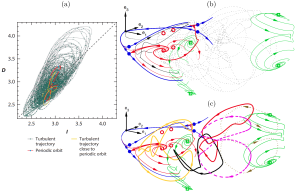
\includegraphics[width=\textwidth]{Background/Figures/BuildingBlocks.pdf}
    \caption{(a) Chaotic \DIFdelbeginFL \DIFdelFL{trajectories }\DIFdelendFL \DIFaddbeginFL \DIFaddFL{trajectory }\DIFaddendFL of turbulence of plane Couette flow at $Re = 400$ \DIFdelbeginFL \DIFdelFL{, approaching the }\DIFdelendFL \DIFaddbeginFL \DIFaddFL{drawn in dark green. The yellow turbulent trajectory evolves close to }\DIFaddendFL an unstable periodic orbit \DIFdelbeginFL \DIFdelFL{(}\DIFdelendFL \DIFaddbeginFL \DIFaddFL{in }\DIFaddendFL red\DIFdelbeginFL \DIFdelFL{) highligted as yellow}\DIFdelendFL ,  adopted from \protect\DIFdelbeginFL \DIFdelFL{\mbox{%DIFAUXCMD
\cite{kawahara_periodic_2001}}\hspace{0pt}%DIFAUXCMD
}\DIFdelendFL \DIFaddbeginFL \DIFaddFL{\mbox{%DIFAUXCMD
\citet{kawahara_periodic_2001}}\hspace{0pt}%DIFAUXCMD
}\DIFaddendFL . (b) State space organisation of turbulence \DIFdelbeginFL \DIFdelFL{trajectores }\DIFdelendFL \DIFaddbeginFL \DIFaddFL{trajectories }\DIFaddendFL (black dots) confined around equilibria (circles, dots and squares) and their unstable manifolds (solid lines), heteroclinic connections between them are shown in red. The coordinate system, $(e_{1,2,3})$, is centered on the laminar state, using a linear combination of the upper branch invariant state. (c) State space projection of five periodic orbits (coloured solid lines), embedded within the same space where turbulence evolves in (b), adopted from \protect\DIFdelbeginFL \DIFdelFL{\mbox{%DIFAUXCMD
\cite{cvitanovic_geometry_2010}}\hspace{0pt}%DIFAUXCMD
}\DIFdelendFL \DIFaddbeginFL \DIFaddFL{\mbox{%DIFAUXCMD
\citet{cvitanovic_geometry_2010}}\hspace{0pt}%DIFAUXCMD
}\DIFaddendFL .}
    \label{fig:BuildingBlocks}
\end{figure}

A major development came with the identification of a pair of non-trivial, unstable equilibrium states in plane Couette flow \citep{nagata_three-dimensional_1990}.
This pair \DIFaddbegin \DIFadd{is }\DIFaddend referred to as the \textit{lower} and \textit{upper} branches, emerging from a saddle node bifurcation disconnected from the stable laminar state.
%DIF <  In the context of parallel shear flows, Nagata was the first to discover a pair of unstable equilibirum solutions in plane Couette flow by smoothly following (homotopy) from a Taylor-Couette configuration \citep{nagata_three-dimensional_1990}.
%DIF <  This pair consist of an unstable upper branch and lower branch emerging as a saddle-node bifurcation near $Re \approx 500$, and is disconnected from the stable laminar solution.
The \textit{lower} branch lies closer to the laminar state, while the \textit{upper} branch resides further away in state space.
% The lower branch refers to its proximity towards the stable laminar state in phase space.
Later, a travelling-wave solution in plane Couette flow \DIFdelbegin \DIFdel{also later }\DIFdelend \DIFaddbegin \DIFadd{was also }\DIFaddend found by the same author \citep{nagata_three-dimensional_1997}.
A family of equilibrium and travelling-wave solutions \DIFdelbegin \DIFdel{was found later }\DIFdelend for plane Couette and plane Poiseuille flows \DIFdelbegin \DIFdel{under }\DIFdelend \DIFaddbegin \DIFadd{with }\DIFaddend different boundary conditions (i.e.\DIFaddbegin \DIFadd{, }\DIFaddend stress-free, slip\DIFaddbegin \DIFadd{, }\DIFaddend and no-slip) \DIFdelbegin \DIFdel{were identified by \mbox{%DIFAUXCMD
\citep{waleffe_exact_2001,waleffe_homotopy_2003}}\hspace{0pt}%DIFAUXCMD
}\DIFdelend \DIFaddbegin \DIFadd{was later identified by \mbox{%DIFAUXCMD
\citet{waleffe_exact_2001} }\hspace{0pt}%DIFAUXCMD
and \mbox{%DIFAUXCMD
\citet{waleffe_homotopy_2003}}\hspace{0pt}%DIFAUXCMD
}\DIFaddend .
Additional equilibria and travelling-wave solutions were identified by \DIFdelbegin \DIFdel{\mbox{%DIFAUXCMD
\cite{gibson_visualizing_2008,gibson_equilibrium_2009}}\hspace{0pt}%DIFAUXCMD
}\DIFdelend \DIFaddbegin \DIFadd{\mbox{%DIFAUXCMD
\citet{gibson_visualizing_2008} }\hspace{0pt}%DIFAUXCMD
and \mbox{%DIFAUXCMD
\citet{gibson_equilibrium_2009}}\hspace{0pt}%DIFAUXCMD
}\DIFaddend , along with \DIFdelbegin \DIFdel{their }\DIFdelend heteroclinic connections between them \citep{halcrow_heteroclinic_2009}.
In the context of pipe flow, multiple travelling-wave solutions have also been reported 
\citep{faisst_traveling_2003,wedin_exact_2004,kerswell_recurrence_2007,wang_lower_2007,duguet_transition_2008,pringle_highly_2009}.
The \DIFdelbegin \DIFdel{set of equilibria, and travelling waves, shows good agreement with the }\DIFdelend statistical quantities (e.g. mean and fluctuations) \DIFdelbegin \DIFdel{with }\DIFdelend \DIFaddbegin \DIFadd{computed from the set of equilibria and travelling waves are in good agreement with those obtained from }\DIFaddend direct numerical simulations.
However, since \DIFdelbegin \DIFdel{they }\DIFdelend \DIFaddbegin \DIFadd{these solutions are }\DIFaddend time independent (within a moving reference frame for travelling waves), they do \DIFdelbegin \DIFdel{no }\DIFdelend \DIFaddbegin \DIFadd{not }\DIFaddend capture the temporal dynamics of turbulence such as the \textit{self-sustaining process} (SSP) \citep{hamilton_regeneration_1995} (see \S \ref{subsec:SSP}).
\DIFdelbegin \DIFdel{While these unstable solutions demonstrate good agreements with results from DNS such as the spanwise length scales, and mean and fluctuations, they do not capture the dynamical processes.
}\DIFdelend 


The next breakthrough was \DIFdelbegin \DIFdel{on the idenfitification }\DIFdelend \DIFaddbegin \DIFadd{the identification }\DIFaddend of time-dependent unstable solutions in the form of periodic orbits. 
\DIFdelbegin \DIFdel{\mbox{%DIFAUXCMD
\cite{kawahara_periodic_2001} }\hspace{0pt}%DIFAUXCMD
}\DIFdelend \DIFaddbegin \DIFadd{\mbox{%DIFAUXCMD
\citet{kawahara_periodic_2001} }\hspace{0pt}%DIFAUXCMD
}\DIFaddend computed a pair of periodic orbits in plane Couette, with one exhibiting a single regeneration cycle similar to the SSP (see figure \ref{fig:BuildingBlocks}(a)) while the other exhibits mild modulation of streaks.
These periodic orbits are linked by heteroclinic connections.
In plane Poiseuille flow, \DIFdelbegin \DIFdel{\mbox{%DIFAUXCMD
\cite{toh_periodic-like_2003} }\hspace{0pt}%DIFAUXCMD
}\DIFdelend \DIFaddbegin \DIFadd{\mbox{%DIFAUXCMD
\citet{toh_periodic-like_2003} }\hspace{0pt}%DIFAUXCMD
}\DIFaddend also identified periodic orbits displaying bursting behaviour.
Using a Newton–Krylov iteration with a hook-step modification, \DIFdelbegin \DIFdel{\mbox{%DIFAUXCMD
\cite{viswanath_recurrent_2007} }\hspace{0pt}%DIFAUXCMD
computed multiply }\DIFdelend \DIFaddbegin \DIFadd{\mbox{%DIFAUXCMD
\citet{viswanath_recurrent_2007} }\hspace{0pt}%DIFAUXCMD
computed multiple }\DIFaddend relative periodic orbits.
These studies conceptualise that the chaotic trajectories of turbulence \DIFdelbegin \DIFdel{as being }\DIFdelend \DIFaddbegin \DIFadd{are }\DIFaddend embedded within a set of unstable periodic orbits, evolving along their unstable \DIFdelbegin \DIFdel{manifolds }\DIFdelend \DIFaddbegin \DIFadd{manifold }\DIFaddend \citep{viswanath_recurrent_2007,gibson_visualizing_2008,gibson_equilibrium_2009,halcrow_heteroclinic_2009,graham_exact_2021}.
An example is shown in figure \ref{fig:BuildingBlocks}, where the chaotic trajectories in figure \ref{fig:BuildingBlocks}(b), reside within the same state space as the periodic orbits, enclosed by equilibria and their heteroclinic connections shown in figure \ref{fig:BuildingBlocks}(c)\DIFdelbegin \DIFdel{,
The set of }\DIFdelend \DIFaddbegin \DIFadd{.
Chaotic trajectories of turbulence reside in the }\textit{\DIFadd{turbulent attractor}} \DIFadd{contains invariant solutions (e.g. }\DIFaddend equilibria, travelling waves\DIFdelbegin \DIFdel{and their relative counterparts, are referred to as }\textit{\DIFdel{invariant solutions}} %DIFAUXCMD
\DIFdel{offering a building block }\DIFdelend \DIFaddbegin \DIFadd{, periodic orbits, and relative periodic orbits) that provide a building-block }\DIFaddend description of turbulence.
However, they \DIFaddbegin \DIFadd{invariant solutions }\DIFaddend do not provide insight into the transition process, since these solutions already reside in the turbulent attractor.

\begin{figure}[h]
    \centering
    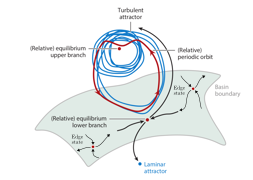
\includegraphics[width=0.8\textwidth]{Background/Figures/EdgeStates.pdf}
    \caption{A graphical representation of the \DIFdelbeginFL \DIFdelFL{edge }\DIFdelendFL \DIFaddbeginFL \textit{\DIFaddFL{basin boundary}} \DIFaddendFL (grey surface) \DIFdelbeginFL \DIFdelFL{separating }\DIFdelendFL \DIFaddbeginFL \DIFaddFL{that seperate }\DIFaddendFL the \DIFdelbeginFL \DIFdelFL{basin }\DIFdelendFL \DIFaddbeginFL \DIFaddFL{basins }\DIFaddendFL of \DIFdelbeginFL \DIFdelFL{boundary }\DIFdelendFL \DIFaddbeginFL \DIFaddFL{attraction }\DIFaddendFL of the laminar and turbulent attractor\DIFdelbeginFL \DIFdelFL{, consisting of }\DIFdelendFL \DIFaddbeginFL \DIFaddFL{. Along the basin boudary sit }\DIFaddendFL attractors, known as edge states, adapted from \protect\DIFdelbeginFL \DIFdelFL{\mbox{%DIFAUXCMD
\cite{graham_exact_2021}}\hspace{0pt}%DIFAUXCMD
}\DIFdelendFL \DIFaddbeginFL \DIFaddFL{\mbox{%DIFAUXCMD
\citet{graham_exact_2021}}\hspace{0pt}%DIFAUXCMD
}\DIFaddendFL .}
    \label{fig:EdgeStates}
\end{figure}
\DIFaddbegin 

\DIFaddend The transition to turbulence in canonical shear flow configurations \DIFdelbegin \DIFdel{are }\DIFdelend \DIFaddbegin \DIFadd{is }\DIFaddend typically subcritical, emerging from the invariant solutions described above, accompanied by an underlying stable laminar state.
A consequence of this is that the laminar and turbulent states form \DIFdelbegin \DIFdel{a }\DIFdelend bistable attractors in phase space with a boundary, separating their respective basins of attraction\DIFaddbegin \DIFadd{, }\DIFaddend known as the \textit{\DIFdelbegin \DIFdel{edge}\DIFdelend \DIFaddbegin \DIFadd{basin boundary}\DIFaddend }.
Attractors that sit along this \DIFdelbegin \DIFdel{edge have been identified and found to possess a saddle-like structure}\DIFdelend \DIFaddbegin \DIFadd{basin boundary were identified as saddles}\DIFaddend , attracting trajectories \DIFdelbegin \DIFdel{within the edge }\DIFdelend \DIFaddbegin \DIFadd{along the basin boundary }\DIFaddend and repelling them toward either \DIFaddbegin \DIFadd{towards }\DIFaddend the laminar or turbulent state, known as \textit{edge \DIFdelbegin %DIFDELCMD < \MBLOCKRIGHTBRACE %%%
\DIFdelend states\DIFaddbegin }\DIFaddend .
The bisection algorithm \DIFdelbegin \DIFdel{used }\DIFdelend for edge tracking \DIFdelbegin \DIFdel{, was first employed in pipe flow experiments by \mbox{%DIFAUXCMD
\cite{schneider_turbulence_2007}}\hspace{0pt}%DIFAUXCMD
, was identified }\DIFdelend \DIFaddbegin \DIFadd{was first applied to pipe-flow experiments by \mbox{%DIFAUXCMD
\citet{schneider_turbulence_2007}}\hspace{0pt}%DIFAUXCMD
.
The edge state was found }\DIFaddend to be chaotic. 
\DIFdelbegin \DIFdel{Time-averaging of this chaotic attractor revealed a close resemblance }\DIFdelend \DIFaddbegin \DIFadd{It was shown that the time-averaged edge state is similar }\DIFaddend to the unstable \DIFdelbegin \DIFdel{lower branch }\DIFdelend \DIFaddbegin \DIFadd{lower-branch }\DIFaddend travelling-wave solutions, suggesting that the \DIFdelbegin \DIFdel{edge separating basin of attraction between the laminar and turbulent states consist of the }\DIFdelend \DIFaddbegin \DIFadd{basin boundary contains }\DIFaddend lower branch solutions and their symmetries \DIFaddbegin \DIFadd{in pipe flows }\DIFaddend \citep{duguet_transition_2008,pringle_highly_2009}.
As \DIFaddbegin \DIFadd{the }\DIFaddend Reynolds number increases, the \DIFdelbegin \DIFdel{edge }\DIFdelend \DIFaddbegin \DIFadd{separation between the edge state }\DIFaddend and the turbulent attractor moves apart \citep{schneider_edge_2009}.
\DIFdelbegin \DIFdel{In the context of pipe flows, it was recognised that the edge consists of a set of unstable lower branch travelling-wave solutions.
}\DIFdelend A graphical representation of the \DIFdelbegin \DIFdel{edge, }\DIFdelend \DIFaddbegin \DIFadd{basin boundary }\DIFaddend and edge states \DIFdelbegin \DIFdel{, separating the laminar the }\DIFdelend \DIFaddbegin \DIFadd{separating the basin of attractions of the laminar and }\DIFaddend turbulent states is shown in figure \ref{fig:EdgeStates}.
\DIFaddbegin 

\DIFaddend Near the onset of subcritical turbulence, turbulence \DIFdelbegin \DIFdel{appear }\DIFdelend \DIFaddbegin \DIFadd{appears }\DIFaddend to be transient, decaying towards the laminar solution after a finite lifetime \citep{bottin_discontinuous_1998,faisst_sensitive_2004,hof_finite_2006}%DIF <  \red{This is often interpreted as the turbulent chaotic attractor colliding with the lower branch solution through a \textit{boundary crisis} \citep{lai_transient_2011}, where the chaotic attractor becomes \textit{leaky}, providing a pathway towards relaminarisation observed in pipe flows \citep{mellibovsky_travelling_2012}, plane Coutte flow \citep{kreilos_periodic_2012} and plane Poiseuille flow \citep{zammert_crisis_2015}.}
%DIF <  \red{This is often interpreted as the turbulent chaotic attractor colliding with the lower branch solution through a \textit{boundary crisis} \citep{lai_transient_2011}, where solution trajectories may `leak' (relaminarise) towards the laminar state in pipe flows \citep{mellibovsky_travelling_2012}, plane Couette flow \citep{kreilos_periodic_2012} and Poiseuille flow \citep{zammert_crisis_2015}.}
\DIFdelbegin \DIFdel{This }\DIFdelend \DIFaddbegin \DIFadd{.
From a dynamical-system perspective, this }\DIFaddend can be interpreted as the turbulent chaotic attractor colliding with the lower branch solution \DIFdelbegin \DIFdel{through }\DIFdelend \DIFaddbegin \DIFadd{known as }\DIFaddend a \textit{boundary crisis} \citep{lai_transient_2011}, forming a \DIFdelbegin \DIFdel{chaotic saddle }\DIFdelend \DIFaddbegin \textit{\DIFadd{chaotic saddle}} \DIFaddend where solution trajectories may \DIFdelbegin \DIFdel{`leak ' }\DIFdelend \DIFaddbegin \DIFadd{leak }\DIFaddend (relaminarise) towards the laminar state \citep{mellibovsky_travelling_2012, kreilos_periodic_2012, zammert_crisis_2015}.
The onset \DIFaddbegin \DIFadd{of }\DIFaddend a boundary crisis (transient turbulence) \DIFdelbegin \DIFdel{have been also }\DIFdelend \DIFaddbegin \DIFadd{has also been }\DIFaddend attributed to the emergence of homoclinic tangency in plane Couette flow \citep{van_veen_homoclinic_2011,lustro_onset_2019}.
%DIF <  where solutiont trajectories could leak towards the laminar state after spending a considerable amount of time in the turbulent attractor.
%DIF <  wandering around the set of invariant solutions along the edge, before falling back onto the laminar state.
\DIFdelbegin %DIFDELCMD < 

%DIFDELCMD < %%%
%DIF <  Turbulent trajectories to appear to be embedded within a collection of unstable periodic orbits, evolving along their unstable manifolds \citep{viswanath_recurrent_2007, gibson_visualizing_2008}
%DIF <  These studies conceptualise chaotic turbulent trajectories as being embedded within a set of unstable periodic orbits, evolving along their unstable manifolds \citep{viswanath_recurrent_2007,gibson_visualizing_2008,gibson_equilibrium_2009,halcrow_heteroclinic_2009,graham_exact_2021}.
%DIFDELCMD < 

%DIFDELCMD < %%%
%DIF <  Chaotic trajectories appear to be embedded within a network of unstable periodic (and relative periodic) orbits and their heteroclinic connections.
%DIFDELCMD < 

%DIFDELCMD < %%%
%DIF <  The chaotic trajectories of turbulence have been found to be embedded within invariant solutions and their connections between them known as heteroclinic orbits, offering a robust view of the building-blocks of of turbulence \citep{gibson_visualizing_2008, gibson_equilibrium_2009, viswanath_recurrent_2007, halcrow_heteroclinic_2009, graham_exact_2021}
%DIFDELCMD < 

%DIFDELCMD < %%%
%DIF <  In the context of this transitional flows, the lower branch solution can be though of separating the turbulent attractor from the laminar state.
%DIF <  Its an attractor that resides on the edge of turbulence, defined as an edge state.
%DIF <  The graphical representation of this edge is shown in figure \ref{fig:StateSpaceGraham}.
%DIFDELCMD < 

%DIFDELCMD < %%%
%DIF <  Coherent structures and turbulent motions
%DIF <  These invariant solutions commonly take the form of as equilibria, travelling waves, periodic and relative periodic orbits.
%DIF <  It is well established that coherent motions defined by flow patterns that persist in space and time play an important role in the transport of momentum and heat.
%DIF <  In parallel shear flows, these coherent structures typically appear as near-walls streaks and quasi-streamwise rollers.
%DIF <  A persistent, quasi-periodic cycle between the regeneration of streaks and rolls, referred to as the \emph{self-sustaining process}, appears to be a fundamental mechanism in sustaining wall-bounded turbulence \emph{self-sustaining process} \citep{hamilton_regeneration_1995}.
%DIF <  This mechanism is described by the generation of streaks due to quasi-streamwise rollers by redistributing the mean.
%DIF <  These streaks become linearly unstable and breakdown, and through a nonlinear process regenerates the quasi-streamwise rollers, closing the cycle.
%DIFDELCMD < 

%DIFDELCMD < %%%
%DIF <  Utilising tools from nonlinear dynamics systems, turbulence could be viewed as chaotic trajectories around unstable nonlinear solutions known as invariant solutions or exact coherent structures \citep{Waleffe_2001,Waleffe_2003,toh2003periodic,Kreilos_2012,nagata2013mirror,Wall_Nagata_2016,Zammert_Eckhardt_2014,graham21}.
\DIFdelend 

%%%%%%%%%%%%%%%%%%%%%%%%%%%%%%%%%%%
% The self-sustaining process 
%%%%%%%%%%%%%%%%%%%%%%%%%%%%%%%%%%%
\subsection{Self-sustaining process}\label{subsec:SSP}
\begin{figure}[h]
    \centering
    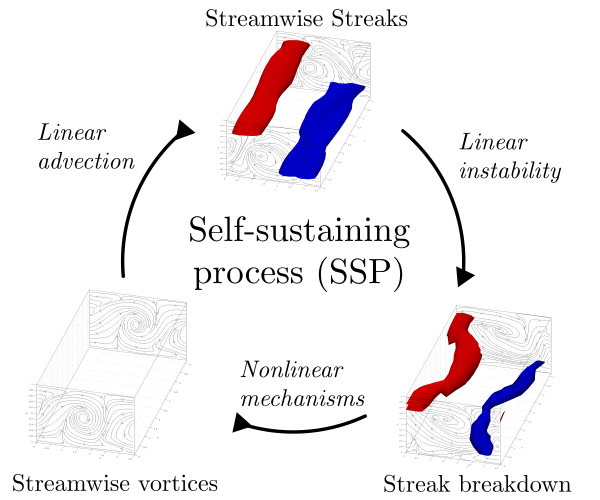
\includegraphics[width=0.7\textwidth]{Background/Figures/SSP/SSP.pdf}
    \caption{The self-sustaining process, consisting of three phases: (1) Streak formation from linear advection by streamwise vortices, (2) streak breakdown due to streak instability and (3) regeneration of streamwise vortices via nonlinear mechanisms.}
    \label{fig:SSP}
\end{figure}

The self-sustaining process (SSP) \DIFdelbegin \DIFdel{describe }\DIFdelend \DIFaddbegin \DIFadd{describes }\DIFaddend the dynamical interaction between a pair of streaks and quasi-streamwise vortices, \DIFdelbegin \DIFdel{considered to be }\DIFdelend \DIFaddbegin \DIFadd{which is considered }\DIFaddend the fundamental process \DIFdelbegin \DIFdel{of wall bounded }\DIFdelend \DIFaddbegin \DIFadd{in wall-bounded }\DIFaddend turbulent flows in the \DIFdelbegin \DIFdel{near wall }\DIFdelend \DIFaddbegin \DIFadd{near-wall }\DIFaddend region.
It is defined by a quasi-cyclic process, consisting of three distinct phases: (1) the formation of streamwise streaks due to a linear advection by streamwise vortices, (2) the wavy breakdown of streaks due to linear instability and (3) the regeneration of streamwise vortices via nonlinear mechanisms \DIFdelbegin \DIFdel{\mbox{%DIFAUXCMD
\citep{durst_origin_1993,waleffe_self-sustaining_1997,hamilton_regeneration_1995}}\hspace{0pt}%DIFAUXCMD
}\DIFdelend \DIFaddbegin \DIFadd{\mbox{%DIFAUXCMD
\citep{durst_origin_1993,hamilton_regeneration_1995,waleffe_self-sustaining_1997}}\hspace{0pt}%DIFAUXCMD
}\DIFaddend .
A schematic of the SSP is shown in figure \ref{fig:SSP}.
While early investigations of the SSP \DIFdelbegin \DIFdel{was confined }\DIFdelend \DIFaddbegin \DIFadd{were confined to }\DIFaddend the buffer layer \citep{hamilton_regeneration_1995}, evidence that the SSP extends towards the logarithmic and outer region has been found \citep{cossu_self-sustaining_2017}.
In parallel to the SSP, the vortex-wave interaction (VWI) theory developed to describe the sustained interactions between a general class of vortices and waves for asymptotically large Reynolds number \DIFdelbegin \DIFdel{\mbox{%DIFAUXCMD
\citep{hall_nonlinear_1988,hall_strongly_1991,stewart_near-planar_1990}}\hspace{0pt}%DIFAUXCMD
}\DIFdelend \DIFaddbegin \DIFadd{\mbox{%DIFAUXCMD
\citep{hall_nonlinear_1988,stewart_near-planar_1990,hall_strongly_1991}}\hspace{0pt}%DIFAUXCMD
}\DIFaddend , was found to be linked to the SSP \citep{hall_streamwise_2010}.
In particular, the solutions obtained using VWI theory by \DIFdelbegin \DIFdel{\mbox{%DIFAUXCMD
\cite{hall_streamwise_2010} }\hspace{0pt}%DIFAUXCMD
is analagous }\DIFdelend \DIFaddbegin \DIFadd{\mbox{%DIFAUXCMD
\citet{hall_streamwise_2010} }\hspace{0pt}%DIFAUXCMD
are analogous }\DIFaddend to the lower branch \DIFdelbegin \DIFdel{solution from \mbox{%DIFAUXCMD
\cite{wang_lower_2007}}\hspace{0pt}%DIFAUXCMD
}\DIFdelend \DIFaddbegin \DIFadd{solutions from \mbox{%DIFAUXCMD
\citet{wang_lower_2007}}\hspace{0pt}%DIFAUXCMD
}\DIFaddend .

%%%%%%%%%%%%%%%%%%%%%%%%%%%%%%%%%%%
% Spatiotemporal transitional flows
%%%%%%%%%%%%%%%%%%%%%%%%%%%%%%%%%%%

\subsection{Spatiotemporal transitional flows}
\begin{figure}[h]
    \centering
    \DIFdelbeginFL %DIFDELCMD < \includegraphics[width=\textwidth]{Background/Figures/Re1400.pdf}
%DIFDELCMD <     %%%
\DIFdelendFL \DIFaddbeginFL \includegraphics[width=1.05\textwidth]{Background/Figures/Re1400.pdf}
    \DIFaddendFL \caption{A snapshot of turbulent-laminar bands at $Re = 1400$ in a large domain $L/h = 16\pi$, depecting its spatiotemporal intermittent nature. Isovolume renderings \DIFdelbeginFL \DIFdelFL{is }\DIFdelendFL \DIFaddbeginFL \DIFaddFL{are }\DIFaddendFL based on the spanwise, $u'$, and wall-normal, $v'$, perturbation kinetic energy, $E(u',v') = 1/2(u'^2 + v'^2)$, where the perturbation velocities are defined about the laminar state $\mathbf{u}'(\mathbf{x},t) = \mathbf{u}(\mathbf{x},t) - U_{lam}(y)$.}
    \label{fig:turbulent-laminar}
\end{figure}

This section describes the inherent spatiotemporal structure of subcritical turbulence near the onset commonly reported in large extended domains.
%DIF <  where the span is about fifty times the half-height of a plane Poiseuille channel, $L/h \gtrsim 50$.
In this regime, turbulence is characterised by the coexistence of turbulent and laminar \DIFaddbegin \DIFadd{flow }\DIFaddend structures.
Examples of such are found in canonical shear flow systems such as plane Couette flows \citep{prigent_long-wavelength_2003,barkley_computational_2005,barkley_mean_2007,tuckerman_patterns_2011,duguet_formation_2010,reetz_exact_2019}, Taylor-Couette flows \citep{prigent_barber_2002,prigent_long-wavelength_2003}, pipe flows \citep{avila_transient_2010,avila_onset_2011,song_speed_2017,avila_transition_2023} and plane Poiseuille flows \citep{tsukahara_dns_2014, tsukahara_dns_2014-1, tuckerman_turbulent-laminar_2014, tsukahara_experimental_2014, gome_statistical_2020, paranjape_onset_2019, paranjape_oblique_2020, paranjape_direct_2023}.

We will focus on the plane Poiseuille flow configuration, where the spatiotemporal intermittent patterns are referred to as oblique turbulent-laminar bands illustrated in figure \ref{fig:turbulent-laminar} at $Re = 1400$ for $L/h = 16\pi$.
The bright and dark regions \DIFdelbegin \DIFdel{highlights coexisting spatially localised }\DIFdelend \DIFaddbegin \DIFadd{highlight coexisting spatially-localised }\DIFaddend turbulent and laminar regions.
These turbulent-laminar bands occur over a range of Reynolds numbers, and \DIFdelbegin \DIFdel{its }\DIFdelend \DIFaddbegin \DIFadd{their }\DIFaddend precise range is dependent on the domain's aspect ratio \citep{tsukahara_experimental_2014,tuckerman_turbulent-laminar_2014,paranjape_direct_2023}.
Near the upper $Re$ threshold of this regime, the domain is fully engulfed by uniform, featureless turbulence appearing at $Re = 1800$ in figure \ref{fig:turbulent-laminar}\DIFdelbegin \DIFdel{(a)}\DIFdelend .
As $Re$ decreases towards $Re = 1050$, spatiotemporal turbulent and laminar structures known as turbulent-laminar bands persist in between $Re \in [1050, 1600]$ shown in figures \ref{fig:turb_lam_bands}(b-f).
In particular, these turbulent-laminar \DIFaddbegin \DIFadd{bands }\DIFaddend appear to have a preferred inclined angle, between $20^\circ \sim 30^\circ$, with streamwise wavelengths of $\lambda_x \sim 60h$, and spanwise wavelengths of $\lambda_z \sim 20h-30h$ \citep{tsukahara_experimental_2014}.
\DIFdelbegin \DIFdel{\mbox{%DIFAUXCMD
\cite{kashyap_linear_2022} }\hspace{0pt}%DIFAUXCMD
}\DIFdelend \DIFaddbegin \DIFadd{\mbox{%DIFAUXCMD
\citet{kashyap_linear_2022} }\hspace{0pt}%DIFAUXCMD
}\DIFaddend considered the linear response of the fluctuating turbulent field, and showed that the preferred band angle emerges near $23.2^\circ$.
%DIF <  Inspired from previous studies of turbulent-laminar bands in plane Couette flows \citep{barkley_computational_2005, reetz_exact_2019}, the minimal band unit (MBU) was employed for plane Poiseuille flows \citep{tuckerman_turbulent-laminar_2014, paranjape_oblique_2020, paranjape_direct_2023}.
%DIF <  In MBUs of plane Poiseuille flows, the turbulent-bands convect at about $\sim1\%$ of the bulk velocity, propagating either upstream or downstream, above or below an critical $Re \sim 1000$, independent of domain sizes for $L_z \geq 100h$ \citep{tuckerman_turbulent-laminar_2014,gome_statistical_2020}.
In the minimal band unit (MBU) studies of plane Poiseuille flows, the \DIFdelbegin \DIFdel{turbulent-bands }\DIFdelend \DIFaddbegin \DIFadd{turbulent-laminar bands }\DIFaddend convect at about $\sim1\%$ of the bulk velocity, propagating either upstream or downstream, depending on $Re$ \citep{tuckerman_turbulent-laminar_2014,gome_statistical_2020}.
%DIF <  To study the preference of angles, zzz performed linear stability analysis of bands and showed that preferred angle at .. degrees.
Notably, the spanwise lengths of the bands are much wider than the half-heights and \DIFdelbegin \DIFdel{depends }\DIFdelend \DIFaddbegin \DIFadd{depend }\DIFaddend on $Re$, appearing at $\lambda_z \sim 20h$ for $Re \gtrsim 1400$ and $\lambda_z \sim 40h$ for $Re \lesssim 1100$.
Interestingly, the bands alternate between both spanwise lengths \DIFdelbegin \DIFdel{between the $Re$ range}\DIFdelend \DIFaddbegin \DIFadd{within $1100 \lesssim Re \lesssim 1400$ }\DIFaddend , merging and splitting continuously \citep{tuckerman_turbulent-laminar_2014}, reminiscent of a puff splitting \DIFdelbegin \DIFdel{\red{process} }\DIFdelend \DIFaddbegin \DIFadd{process }\DIFaddend in pipe flows \citep{avila_onset_2011}.
An example of this could been observed in $Re = 1050$, where the band appears to alternate between different spanwise wavelengths in figure \ref{fig:turb_lam_bands}(f).
% Below certain $Re$ threshold, the spatially turbulent regions decay where the flow relaminarises \citep{tuckerman_turbulent-laminar_2014}.
As $Re$ falls below a certain $Re$ threshold, turbulent bands spontaneously decay and \DIFdelbegin \DIFdel{relaminarises }\DIFdelend \DIFaddbegin \DIFadd{relaminarise }\DIFaddend \citep{tuckerman_turbulent-laminar_2014,gome_statistical_2020}.
An example is shown in figure \ref{fig:turb_lam_bands}(g).
% An example of this decay is shown in $Re = 1000$ near $t = 1600$ in figure \ref{fig:turb_lam_bands}(g). 
\begin{figure}[h]
    \centering
    \includegraphics[width=\textwidth]{Background/Figures/Ra0-BotSpaceTime.pdf}
    \caption{Turbulent-laminar bands for $t \in [0, 3000]$ in large domains $(L_x, L_z) = (16\pi, 16\pi)$ at (a) $Re = 1800$, (b) $Re = 1600$, (c) $Re = 1400$,  (d)  $Re =1200$, (e) $Re = 1100$, (f) $Re = 1050$,  (g) $Re = 1000$.}
    \label{fig:turb_lam_bands}
\end{figure}

\begin{figure}[h]
    \centering
    \includegraphics[width=0.7\textwidth]{Background/Figures/gome_prob.pdf}
    \caption{The mean decay times (red), $\tau^d$, and mean splitting times (black), $\tau^s$, as a function of Reynolds number, leading to a crossover point at $Re_{cross} \approx 965$, adapted from \protect\DIFdelbeginFL \DIFdelFL{\mbox{%DIFAUXCMD
\cite{gome_statistical_2020}}\hspace{0pt}%DIFAUXCMD
}\DIFdelendFL \DIFaddbeginFL \DIFaddFL{\mbox{%DIFAUXCMD
\citet{gome_statistical_2020}}\hspace{0pt}%DIFAUXCMD
}\DIFaddendFL .}
    \label{fig:decay_split_probability}
\end{figure}

%DIF <  As $Re$ is lowered turbulent bands appear to decay at $Re = 830$ \citep{gome_statistical_2020}, and at $Re = 1100$ but surviving for $Re = 1000$ \citep{tuckerman_turbulent-laminar_2014}, suggesting that turbulent bands decay spontaneously.
%DIF <  However, at $Re = 1100$ but surviving for $Re = 1000$ \citep{tuckerman_turbulent-laminar_2014}, suggesting that turbulent bands decay spontaneously.
\DIFdelbegin \DIFdel{\mbox{%DIFAUXCMD
\cite{gome_statistical_2020} }\hspace{0pt}%DIFAUXCMD
computed the probabilities }\DIFdelend \DIFaddbegin \DIFadd{\mbox{%DIFAUXCMD
\citet{gome_statistical_2020} }\hspace{0pt}%DIFAUXCMD
computed the probability }\DIFaddend distributions for turbulent-laminar band decay, $P(\Delta t^d)$, where $\Delta t^d$ is the time until decay.
A key insight is that the probability \DIFdelbegin \DIFdel{distributions }\DIFdelend \DIFaddbegin \DIFadd{distribution }\DIFaddend of turbulent band decay \DIFdelbegin \DIFdel{mimics }\DIFdelend \DIFaddbegin \DIFadd{is }\DIFaddend a memoryless Poisson process,
\begin{equation}
    P(\Delta t^d) = \exp(-\Delta t^d/\tau^d(Re)),
\end{equation}
where $\tau^d(Re)$ refers to the mean lifetime for decay as a function of $Re$.
Similarly, the band splitting process also \DIFdelbegin \DIFdel{follow }\DIFdelend \DIFaddbegin \DIFadd{follows }\DIFaddend a Poisson process,
\begin{equation}
    P(\Delta t^s) = \exp(-\Delta t^s / \tau^s(Re)),
\end{equation}
\DIFdelbegin \DIFdel{white }\DIFdelend \DIFaddbegin \DIFadd{while }\DIFaddend $\tau^s(Re)$ \DIFaddbegin \DIFadd{is }\DIFaddend the mean splitting lifetime.
%DIF <  the probability distribution for band splitting also follows a Poisson distribution, , where $\tau^s(Re)$ refers to the mean lifetime of a splitting event dependent on $Re$.
Both $\tau^d$ and $\tau^s$ exhibit superexponential dependence on $Re$, \DIFdelbegin \begin{displaymath}
    \DIFdel{\tau^{d,s} = \exp(\exp(Re)),
}\end{displaymath}%DIFAUXCMD
%DIF <  The mean survival lifetime of a band decaying, $\tau^d$, and splitting, $\tau^s$, depends superexponentially on $Re$, i.e. $\tau^{d,s} = \exp(\exp(Re))$.
\DIFdel{This is }\DIFdelend shown in figure \ref{fig:decay_split_probability} \DIFdelbegin \DIFdel{, with a crossover pointat }\DIFdelend \DIFaddbegin \DIFadd{(see inset).
The crossover point, }\DIFaddend $Re_{cross} \approx 965$, where both \DIFaddbegin \DIFadd{band }\DIFaddend decay and splitting \DIFdelbegin \DIFdel{becomes equally probable.
This crossover point is considered as }\DIFdelend \DIFaddbegin \DIFadd{events become equally probable, is considered }\DIFaddend the critical Reynolds number for the onset of \DIFdelbegin \DIFdel{turbulent bands.
%DIF <  By extrapolating the estimated mean lifetimes of a splitting and decay event, the crossing point (i.e equal chance of identifying a splitting and decay event after a time-scale of $t = 3 \times 10^6$) occurs at $Re_{cross} \approx 965$, in other words, $Re_{cross}$ acts as a critical Reynolds number.
}\DIFdelend \DIFaddbegin \DIFadd{turbulent-laminar bands.
}\DIFaddend 

While there has been progress made towards our understanding of infinitely bi-periodic turbulent-laminar bands in MBUs, recent studies of isolated (non-periodic) turbulent bands (ITBs) reveal different behaviour.
Notably, ITBs persist at Reynolds number below $Re_{cross}$ at $Re = 700$ for durations exceeding $t = 10000$, exceeding the mean decay lifetime in figure \ref{fig:decay_split_probability}.
The ITBs are characterised by \DIFdelbegin \DIFdel{streak generating }\DIFdelend \DIFaddbegin \DIFadd{a streak-generating }\DIFaddend head and a \DIFdelbegin \DIFdel{diffusive }\DIFdelend \DIFaddbegin \DIFadd{diffuse }\DIFaddend upstream tail. \citep{xiong_turbulent_2015, tao_extended_2018, shimizu_bifurcations_2019, xiao_growth_2020}.
\DIFdelbegin \DIFdel{We conclude our discussion  on transitional wall-bounded shear flows.
%DIF <  It is worth noting that isolated bands are not memoryless, depending on their pass history [citation]
%DIF <  Above a certain Reynolds number, the probability of band splitting again depends on a super-exponentianal.
%DIF <  Show graph.
%DIF <  In the context of plane Poiseuille flowsd, it is well known that at $Re \sim 1000 - 2000$, turbulence behaves intermittently, existing as oblique bands of turbulent and laminar regions. 
%DIF <  Over the past decade, research efforts have been dedicated to the study of turbulent-laminar bands.
}%DIFDELCMD < 

%DIFDELCMD < %%%
%DIF <  At $Re \sim 1000 - 2000$, turbulent bands can either decay spontaneously, stabilising into a laminar state, or split, forming more bands whereby turbulent-laminar bands are sustained.
%DIF <  The probability of decay and splitting lifetimes strongly depends on the domain size and $Re$.
%DIF <  At $L_z = 100h$, the critical Reynolds number of $Re_{cr} \approx 965$ have been determined statistically, whereby decay and splitting lifetimes intersect more than $10^6$ advective time units. 
%DIF <  It is worth to note that for $Re < Re_{cr}$, the probably of decay is higher than splitting events, vice versa. 
\DIFdelend 


%%%%%%%%%%%%%%%%%%%%%%%%%%%%
% Rayleigh Benard Convection
%%%%%%%%%%%%%%%%%%%%%%%%%%%%

\section{Rayleigh-B\'{e}nard convection}\label{sec:bkgrd_RBC}

\begin{figure}[h]
    \centering
    \includegraphics[width=\textwidth]{Background/Figures/BenardCells.png}
    \caption{(a) Surface tension driven convection leading to the onset of hexagonal B\'{e}nard cells in a thin layer of silicone oil, heated from below and cooled by ambient air. A diamond defect appears, likely caused by plate imperfections. (b) Buoyancy driven convection \DIFdelbeginFL \DIFdelFL{in }\DIFdelendFL \DIFaddbeginFL \DIFaddFL{between }\DIFaddendFL rigid plates, resulting \DIFdelbeginFL \DIFdelFL{to }\DIFdelendFL \DIFaddbeginFL \DIFaddFL{in }\DIFaddendFL concentric convection rolls at $2.9$ times the critical Rayleigh number. Both experiments were performed by \protect\DIFdelbeginFL \DIFdelFL{\mbox{%DIFAUXCMD
\cite{koschmieder_heat_1974}}\hspace{0pt}%DIFAUXCMD
}\DIFdelendFL \DIFaddbeginFL \DIFaddFL{\mbox{%DIFAUXCMD
\citet{koschmieder_heat_1974}}\hspace{0pt}%DIFAUXCMD
}\DIFaddendFL , and the convection patterns were illuminated by aluminum powder, where the dark and bright regions refer to vertical and horizontal motions \DIFdelbeginFL \DIFdelFL{resepctively}\DIFdelendFL \DIFaddbeginFL \DIFaddFL{respectively}\DIFaddendFL . These higher resolution images were taken from \protect\DIFdelbeginFL \DIFdelFL{\mbox{%DIFAUXCMD
\cite{van1982album}}\hspace{0pt}%DIFAUXCMD
}\DIFdelendFL \DIFaddbeginFL \DIFaddFL{\mbox{%DIFAUXCMD
\citet{van1982album}}\hspace{0pt}%DIFAUXCMD
}\DIFaddendFL .}
    \label{fig:benard_cells}
\end{figure}

Rayleigh-B\'{e}nard convection (RBC) is a paradigmatic fluid configuration describing the motion of the fluid confined between two infinite-parallel plates heated from below and cooled from the top.
% The basic physical mechanism underpinning RBC is variation of buoyancy due to heat, offering a simple description of natural convection.
As the bottom plate is heated, the \DIFdelbegin \DIFdel{bottom layer }\DIFdelend \DIFaddbegin \DIFadd{bottom-layer }\DIFaddend fluid becomes more buoyant and tends to rise, \DIFdelbegin \DIFdel{while the colder top fluid layer is becomes relatively }\DIFdelend \DIFaddbegin \DIFadd{whereas the colder top-layer fluid becomes }\DIFaddend less buoyant and tends to sink, leading to \DIFdelbegin \DIFdel{an overturning of }\DIFdelend \DIFaddbegin \DIFadd{overturning of the }\DIFaddend layers.
Viscous forces between neighbouring fluid parcels act to resist the motion. 
As buoyancy overcomes these viscous forces, the fluid layers overturn, \DIFdelbegin \DIFdel{resulting in the initiation of }\DIFdelend \DIFaddbegin \DIFadd{initiating }\DIFaddend buoyancy-driven convection, the physical mechanism underpinning RBC.

One of the earliest experimental studies dedicated to buoyancy-driven convection was conducted by Henri B\'{e}nard \citep{benard_tourbillons_1901}, who observed the formation of hexagonal convection cells above a certain temperature threshold $\Delta T$.
These hexagonal patterns are referred to as B\'{e}nard cells\DIFdelbegin \DIFdel{are }\DIFdelend \DIFaddbegin \DIFadd{, }\DIFaddend illustrated in figure \ref{fig:benard_cells}(a)\DIFdelbegin \DIFdel{(adapted from \mbox{%DIFAUXCMD
\citep{koschmieder_heat_1974}}\hspace{0pt}%DIFAUXCMD
)}\DIFdelend . 
Subsequently, \DIFdelbegin \DIFdel{\mbox{%DIFAUXCMD
\cite{rayleigh_lix_1916} }\hspace{0pt}%DIFAUXCMD
}\DIFdelend \DIFaddbegin \DIFadd{\mbox{%DIFAUXCMD
\citet{rayleigh_lix_1916} }\hspace{0pt}%DIFAUXCMD
}\DIFaddend carried out one of \DIFaddbegin \DIFadd{the }\DIFaddend first linear stability analyses of buoyancy-driven convection, predicting the onset of convection at a critical Rayleigh number of $Ra_c = 657.5$.
However, Rayleigh's analysis assumed \DIFdelbegin \DIFdel{an }\DIFdelend idealised free-free boundary conditions, which differed from the rigid-free setup of B\'{e}nard's experiment.
The linear stability analysis for \DIFaddbegin \DIFadd{the }\DIFaddend rigid-free configuration was later performed by \DIFdelbegin \DIFdel{\mbox{%DIFAUXCMD
\cite{jeffreys_cases_1928} }\hspace{0pt}%DIFAUXCMD
}\DIFdelend \DIFaddbegin \DIFadd{\mbox{%DIFAUXCMD
\citet{jeffreys_cases_1928}}\hspace{0pt}%DIFAUXCMD
, }\DIFaddend yielding a higher critical Rayleigh number of $Ra_c = 1058$.
In the rigid-rigid configuration, the critical Rayleigh number increases further to $Ra_c = 1708$ \citep{pellew_maintained_1940}.
The Rayleigh number in B\'{e}nard's original experiment contradicted results from linear stability analysis as it was found to be 300 to 1500\DIFaddbegin \DIFadd{, }\DIFaddend smaller than $Ra_c$ for the free-free and rigid-free cases respectively \citep{wesfreid_henri_2017}.
%DIF <  However, it is worth highlighting a key difference in B\'{e}nard's experiment and Rayleigh's analysis.
This contradiction, not recognised by B\'{e}nard at the time, lies in the significant role of surface tension in thin fluid layers exposed to air, now known as B\'{e}nard-Maragoni (BM) convection \citep{block_surface_1956, cloot_nonlinear_1984, hohler_rayleigh-benard_2006, wesfreid_henri_2017}.
In BM convection, fluid motion is primarily driven by surface tension gradients due to variations of temperature, forming hexagonal cells, as in figure \ref{fig:benard_cells}(a).
The preference for hexagonal cells in BM convection was later confirmed based on weakly nonlinear stability analysis \citep{cloot_nonlinear_1984}.
%DIF <  as in B\'{e}nard experiments, a thin layer of fluid exposed to the air is chiefly driven by the variation of surface tension due to temperature difference, leading to the growth of hexagonal cells, in figure \ref{fig:benard_cells}(a).
As the fluid layer becomes thicker, surface-tension effects diminish and buoyancy-driven convection becomes dominant.
Similarly, placing a rigid lid on top of a thin fluid layer suppresses surface-tension effects, resulting in buoyancy-driven convection (compare between \ref{fig:benard_cells}(a) and (b))
%DIF <  Surface-tension effects diminish as the fluid depth increases, or removed in the presence of a top rigid lid, where buoyancy becomes the dominant mechanism.
The preferred convection patterns based on weakly nonlinear stability analysis are the two-dimensional parallel rolls, now referred to as ideal straight rolls (ISRs) \citep{schluter_stability_1965, bodenschatz_recent_2000}.
%DIF <  This also have the same effect as placing a lid on top of thin layer of fluid where surface-tension effects are removed, leading to ISRs.
%DIF <  This key discrepancy was later identified as B\'{e}nard's experiments considered thin layers of fluid heated and cooled by the ambient air \citep{block_surface_1956}, where surface tension (Maragoni) effects were significant.
\DIFdelbegin \DIFdel{In circular ontainers}\DIFdelend \DIFaddbegin \DIFadd{In circular containers}\DIFaddend , the ISRs conform to the geometry of the boundaries, forming concentric convection rolls illustrated in figure \ref{fig:benard_cells}(b).
Interestingly, \DIFdelbegin \DIFdel{hexgaonal }\DIFdelend \DIFaddbegin \DIFadd{hexagonal }\DIFaddend cells have been observed in buoyancy-driven flows of non-Boussinesq fluids \citep{hoard_experiments_1970,bodenschatz_recent_2000}.
In this thesis, we consider the RBP setup (and RBC in chapter 4) with rigid-rigid boundary conditions \DIFdelbegin \DIFdel{, bearing }\DIFdelend \DIFaddbegin \DIFadd{and a }\DIFaddend critical Rayleigh number of $Ra_c = 1708$.
Notably, the corresponding critical wavelength is $q_c = 3.12 / d$ (or $\lambda_c \approx  2d$), suggesting that \DIFaddbegin \DIFadd{the }\DIFaddend distance separating the plates, $d$, dictates the length of a single roll, $l_{roll} = \lambda_c / 2 \approx d$.
%DIF <  1. Bousinessq fluids (silicon oil) leads to 2D rolls or Hexagonal rolls for rigid-rigid and open-rigid B.Cs - highlighting the importance of the top B.C
%DIF <      a. Are they buoyancy driven or surface-tension driven?
%DIF <  
%DIF <  2. Non-bouseinessq (Aroclor) lead to rigid-rigid boundary conditions lead to rolls for thick layers, and hexes in thin layers. In open-rigid boundary conditions, 2D concentric rolls develop in thick layers while hexagonal cells form in thin layers.
\DIFdelbegin %DIFDELCMD < 

%DIFDELCMD < %%%
%DIF <  While the $Ra_c$ for free-free and rigid-free have been reported \citep{rayleigh_lix_1916,jeffreys_cases_1928}.
%DIF <  It is also worth noting that \cite{rayleigh_lix_1916} considered a stress-free boundary conditions in his analysis, which has been extended to rigid boundary conditions, the critical Rayleigh number increased to well known $Ra_c = 1707.8$ \citep{pellew_maintained_1940}, and is independent or $Pr$ \citep{bodenschatz_recent_2000}.
%DIFDELCMD < 

%DIFDELCMD < %%%
%DIF <  ension decreases  generated a tangential forces towards regions of higher surface tension at the surface, where cold fluid resides, ampliying convection, now known as B\'{e}nard-Maragoni convection \citep{manneville_thirty_2006}. 
%DIF < , with a critical wavenumber of $q_c = \frac{\pi}{\sqrt{2}d}$.
%DIF <  and predicted the critical Rayleigh number of $Ra_c = \frac{27}{4}\pi^4 = 657.5$, and a critical wavelength of $q_c = \frac{\pi}{\sqrt{2}d}$.
%DIF <  where $Ra, \alpha, g, d \Delta T, \kappa, \nu$ refers to the Rayleigh number, volumetric thermal expansion of the fluid, gravitational constant, width and temperature difference between plates, thermal diffusivity and kinematic viscosity. 
%DIF <  When $Ra$ exceeds a certain critical Rayleigh number $Ra_c$, the fluid configuration becomes unstable and convection motion ensures.
%DIF <  The pioneering work from Rayleigh, and B\'{e}nard's experiment formed the early foundations of buoyancy-driven convection, now known as Rayleigh-B\'{e}nard convection.
%DIF <  In the absence of surface tension effects, the critical Rayleigh number, $Ra_c$ depends on the boundary condition, commonly analysed using stress-free or rigid-rigid (no-slip) boundary conditions.
%DIF <  In Rayleigh's work, he considered a stress-free condition at the wall, ${\partial u}/{\partial n} = 0$, where analytical solutions are admittable.
\DIFdelend 

\begin{figure}[t]
    \centering
    \DIFdelbeginFL %DIFDELCMD < \includegraphics[width=0.8\textwidth]{Background/Figures/BusseBalloonFull.png}
%DIFDELCMD <     %%%
\DIFdelendFL \DIFaddbeginFL 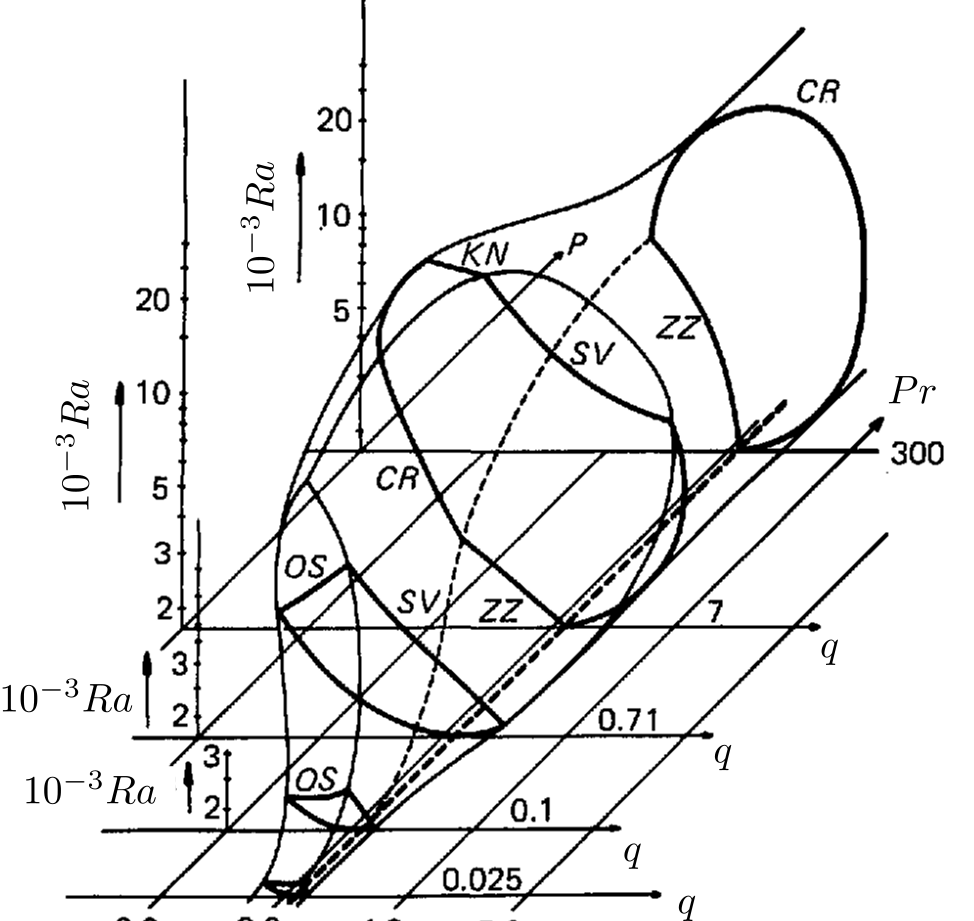
\includegraphics[width=0.8\textwidth]{Background/Figures/BusseBalloon_Busse.png}
    \DIFaddendFL \caption{The Busse \DIFdelbeginFL \DIFdelFL{ballon }\DIFdelendFL \DIFaddbeginFL \DIFaddFL{balloon }\DIFaddendFL describes the stability boundaries of ISRs in a \DIFdelbeginFL \DIFdelFL{$\varepsilon-q$ }\DIFdelendFL \DIFaddbeginFL \DIFaddFL{$Ra-Pr-q$ }\DIFaddendFL space. For \DIFdelbeginFL \DIFdelFL{larger wavenumbers}\DIFdelendFL \DIFaddbeginFL \DIFaddFL{large values of $Pr$}\DIFaddendFL , the instability mechanisms \DIFdelbeginFL \DIFdelFL{is described by }\DIFdelendFL \DIFaddbeginFL \DIFaddFL{are }\DIFaddendFL the \DIFdelbeginFL \DIFdelFL{skewed-varicose }\DIFdelendFL \DIFaddbeginFL \DIFaddFL{cross-roll }\DIFaddendFL (\DIFdelbeginFL \DIFdelFL{SV}\DIFdelendFL \DIFaddbeginFL \DIFaddFL{CR}\DIFaddendFL )\DIFdelbeginFL \DIFdelFL{instability}\DIFdelendFL \DIFaddbeginFL \DIFaddFL{, knotted (KN) and zig-zag (ZZ) instabilities}\DIFaddendFL . For \DIFdelbeginFL \DIFdelFL{smaller wavenumbers}\DIFdelendFL \DIFaddbeginFL \DIFaddFL{$Pr\approx1$}\DIFaddendFL , the instability \DIFdelbeginFL \DIFdelFL{mechanism is described by }\DIFdelendFL \DIFaddbeginFL \DIFaddFL{mechanisms are }\DIFaddendFL the \DIFdelbeginFL \DIFdelFL{Eckhaus }\DIFdelendFL \DIFaddbeginFL \DIFaddFL{skew-varicose (SV) and oscillatory (OS) }\DIFaddendFL instability. For \DIFdelbeginFL \DIFdelFL{large $\varepsilon$}\DIFdelendFL \DIFaddbeginFL \DIFaddFL{small values of $Pr$}\DIFaddendFL , the \DIFaddbeginFL \DIFaddFL{OS }\DIFaddendFL instability \DIFdelbeginFL \DIFdelFL{is described by the onset of oscillatory instability}\DIFdelendFL \DIFaddbeginFL \DIFaddFL{dominants}\DIFaddendFL . \DIFdelbeginFL \DIFdelFL{Busse balloon digitised }\DIFdelendFL \DIFaddbeginFL \DIFaddFL{This figure was modified }\DIFaddendFL from \protect\DIFdelbeginFL \DIFdelFL{\mbox{%DIFAUXCMD
\cite{plapp_spiral_1997} }\hspace{0pt}%DIFAUXCMD
for $Pr \approx 1$}\DIFdelendFL \DIFaddbeginFL \DIFaddFL{\mbox{%DIFAUXCMD
\citet{swinney_transition_1981}}\hspace{0pt}%DIFAUXCMD
}\DIFaddendFL .}
    \label{fig:busseballon}
\end{figure}

As mentioned earlier, stationary ISRs near $q_c$ emerge just above $Ra_c$, based on weakly nonlinear \DIFdelbegin \DIFdel{stabity analysis . }\DIFdelend \DIFaddbegin \DIFadd{stability analysis }\DIFaddend \citep{eckhaus_studies_1965, schluter_stability_1965}.
However, this prediction \DIFaddbegin \DIFadd{is }\DIFaddend contradicted by the emergence of time-dependent oscillatory \DIFdelbegin \DIFdel{ISRs }\DIFdelend \DIFaddbegin \DIFadd{convection rolls }\DIFaddend in experiments \citep{rossby_study_1969,willis_oscillatory_1970} at $Ra = 9200$ (or roughly five times $Ra_c$), where weakly nonlinear stability analysis becomes inapplicable far from threshold.
To address this, \DIFdelbegin \DIFdel{a }\DIFdelend secondary stability analysis was \DIFdelbegin \DIFdel{employed }\DIFdelend \DIFaddbegin \DIFadd{performed }\DIFaddend to study the stability of ISRs further from $Ra_c$ \citep{busse_oscillatory_1972}.
%DIF <  \cite{busse_oscillatory_1972} performed secondary linear stability analysis of ISRs based on Galerkin truncation of orthogonal functions.
One of the key results from this analysis is the Busse balloon, which describes the stability boundaries of ISRs as a function of $Ra$ and $Pr$, and roll wavenumber, \DIFdelbegin \DIFdel{$\alpha$, shown figure \ref{fig:busseballon} \mbox{%DIFAUXCMD
\citep{busse_non-linear_1978}}\hspace{0pt}%DIFAUXCMD
}\DIFdelend \DIFaddbegin \DIFadd{$q$, shown in figure \ref{fig:busseballon} \mbox{%DIFAUXCMD
\citep{swinney_transition_1981}}\hspace{0pt}%DIFAUXCMD
}\DIFaddend .
The boundaries of the Busse balloon are described by a range of secondary instabilities, each arising from different physical mechanisms \citep{busse_non-linear_1978}.
At large Prandtl numbers, $Pr = O(10^2)$, the zig-zag (ZZ) and cross-roll (CR) instabilities \DIFdelbegin \DIFdel{delimits }\DIFdelend \DIFaddbegin \DIFadd{delimit }\DIFaddend the balloon for small and large roll wavenumbers.
The zig-zag instabilities cause zig-zag undulations while the CR instabilities \DIFdelbegin \DIFdel{generates }\DIFdelend \DIFaddbegin \DIFadd{generate }\DIFaddend rolls orthogonal to the underlying ISR structure, effectively increasing or decreasing the roll wavenumber\DIFaddbegin \DIFadd{, }\DIFaddend respectively \citep{busse_instabilities_1971}.
Examples of these instabilities at $Pr = 100$ are illustrated in figure \ref{fig:busseballoon_secinstab}(a,b).

\begin{figure}
    \centering
    \includegraphics[width=0.5\textwidth]{Background/Figures/BusseBalloon/SecondaryInstabilities.pdf}
    \caption{ISRs experiencing (a) cross-roll instability at $Ra = 3000, Pr = 100$ and (b) zig-zag instability at $Ra = 3600, Pr = 100$ \protect\citep{busse_instabilities_1971}. (c) \DIFdelbeginFL \DIFdelFL{Skew-varicosed }\DIFdelendFL \DIFaddbeginFL \DIFaddFL{Skewed-varicose }\DIFaddendFL instability at $Ra = 5568, Pr = 1$ \protect\citep{plapp_spiral_1997}, and (d) oscillatory instability at $Ra = 10384, Pr = 1$ \citep{cakmur_bistability_1997}.}
    \label{fig:busseballoon_secinstab}
\end{figure}

At moderate Prandtl numbers, $Pr = O(1)$, the Busse balloon is bounded by the \DIFdelbegin \DIFdel{skewed varicosed }\DIFdelend \DIFaddbegin \DIFadd{skew-varicose }\DIFaddend (SV) for high roll wavenumbers and the oscillatory (OS) instability at large $Ra$.
%DIF <  The cross-roll instability generates an additional roll orthogonal to the existing roll, while the zig-zag instabilities leads to the emergence of zig-zag ISRs.
\DIFdelbegin \DIFdel{The skewed-varicosed }\DIFdelend \DIFaddbegin \DIFadd{The skew-varicose }\DIFaddend (SV) instability leads to roll-pinching\DIFaddbegin \DIFadd{, }\DIFaddend where pinched rolls merged into a single roll, reducing roll wavenumber\DIFaddbegin \DIFadd{, }\DIFaddend while the oscillatory instability leads to the onset of an oscillatory \DIFdelbegin \DIFdel{ISRs}\DIFdelend \DIFaddbegin \DIFadd{convection roll}\DIFaddend . 
Examples of the respective instabilities at $Pr = 1$ are shown in figure \ref{fig:busseballoon_secinstab}(c,d).
At higher wavenumbers, the \DIFdelbegin \DIFdel{skewed varicose }\DIFdelend \DIFaddbegin \DIFadd{skew-varicose }\DIFaddend (SV) instability becomes relevant at intermediate \DIFdelbegin \DIFdel{Prandlt }\DIFdelend \DIFaddbegin \DIFadd{Prandtl }\DIFaddend numbers, characterised by roll pinching and merging that effectively reduces the roll wavenumber.
% For larger Rayleigh numbers and $Pr \lesssim 1$, the oscillatory instability (OS) arises, forming oscillatory ISRs \citep{willis_oscillatory_1970}.
% In contrast, for higher $Pr$, the knot instability appears, modifying the cross-roll pattern into a spoke-like structure.
Finally, the Eckhaus instability (not shown), \DIFdelbegin \DIFdel{related to the symmetry of the system, appears close to the $Ra_c$, leading a disturbance parallel to the underlying rolls }\DIFdelend which either creates or \DIFdelbegin \DIFdel{destroy }\DIFdelend \DIFaddbegin \DIFadd{destroys }\DIFaddend rolls such that the resultant roll wavenumber \DIFdelbegin \DIFdel{adheres to the stability boundaries }\DIFdelend \DIFaddbegin \DIFadd{moves closer to the critical wavenumber, appears close to $Ra_c$ }\DIFaddend \citep{lowe_pattern_1985}.
Near $Pr = 1$, the Eckhaus instability coincides with the \DIFdelbegin \DIFdel{crossroll }\DIFdelend \DIFaddbegin \DIFadd{cross-roll }\DIFaddend instability (figure 6 from \DIFdelbegin \DIFdel{\mbox{%DIFAUXCMD
\cite{bodenschatz_recent_2000}}\hspace{0pt}%DIFAUXCMD
}\DIFdelend \DIFaddbegin \DIFadd{\mbox{%DIFAUXCMD
\citet{bodenschatz_recent_2000}}\hspace{0pt}%DIFAUXCMD
}\DIFaddend , adapted from \DIFdelbegin \DIFdel{\mbox{%DIFAUXCMD
\cite{plapp_spiral_1997}}\hspace{0pt}%DIFAUXCMD
.)}\DIFdelend \DIFaddbegin \DIFadd{\mbox{%DIFAUXCMD
\citet{plapp_spiral_1997}}\hspace{0pt}%DIFAUXCMD
).
}\DIFaddend 

In this thesis, we focus on fluids with $Pr = 1$, where secondary instabilities such as \DIFdelbegin \DIFdel{skewed-varicose}\DIFdelend \DIFaddbegin \DIFadd{skew-varicose}\DIFaddend , Eckhaus and cross-roll instabilities typically arise.
While the stability boundaries of the Busse balloon have been experimentally verified \citep{busse_instabilities_1971, croquette_convective_1989, plapp_spiral_1997}, accurately predicting the wavenumber of ideal straight rolls (ISRs) \DIFdelbegin \DIFdel{remain }\DIFdelend \DIFaddbegin \DIFadd{remains }\DIFaddend difficult due to hysteresis and the existence of multiple stable ISRs of different roll wavenumbers.
As $Ra$ \DIFdelbegin \DIFdel{continously increases}\DIFdelend \DIFaddbegin \DIFadd{is increased}\DIFaddend , ISRs with wavenumbers outside the Busse Balloon undergo \DIFdelbegin \DIFdel{the }\DIFdelend secondary instabilities (described above) that drive their wavenumbers back \DIFdelbegin \DIFdel{to }\DIFdelend \DIFaddbegin \DIFadd{towards }\DIFaddend the stable boundaries.
%DIF <  These instabilities either increase or decrease the roll wavenumber, adhering to the the stability boundaries of the Busse balloon.
The hysteretic behaviour highlights that the roll wavenumber of \DIFdelbegin \DIFdel{the }\DIFdelend ISRs is strongly dependent on the system's history \citep{bodenschatz_recent_2000}.

% MULTIPLE STATES
It is worth noting that the ISRs are the exception rather than the rule in RBC \citep{croquette_convective_1989-1}.
A range of non-ISR states, such as squares, travelling or stationary target patterns, giant rotating spirals, and oscillatory convection, have been observed over the years \DIFdelbegin \DIFdel{\mbox{%DIFAUXCMD
\citep{le_gal_square_1985, croquette_convective_1989, plapp_spiral_1997, hof_flow_1999, rudiger_pattern_2000, boronska_extreme_2010, boronska_extreme_2010-1}}\hspace{0pt}%DIFAUXCMD
.
%DIF <  The coexistence of multiple ‘non-ISR’ states, in the form of squares, travelling/stationary targets, giant rotating spirals, and oscillatory convection patterns have been found over several years \citep{le_gal_square_1985, croquette_convective_1989, plapp_spiral_1997, hof_flow_1999, rudiger_pattern_2000, boronska_extreme_2010, boronska_extreme_2010-1}.
}\DIFdelend \DIFaddbegin \DIFadd{\mbox{%DIFAUXCMD
\citep{le_gal_square_1985, croquette_convective_1989, plapp_spiral_1997, hof_flow_1999, rudiger_pattern_2000, boronska_extreme_2010_A, boronska_extreme_2010_B}}\hspace{0pt}%DIFAUXCMD
.
}\DIFaddend For example, \DIFdelbegin \DIFdel{\mbox{%DIFAUXCMD
\cite{hof_flow_1999} }\hspace{0pt}%DIFAUXCMD
}\DIFdelend \DIFaddbegin \DIFadd{\mbox{%DIFAUXCMD
\citet{hof_flow_1999} }\hspace{0pt}%DIFAUXCMD
}\DIFaddend identified eight stationary and two oscillatory \DIFdelbegin \DIFdel{state in cylinderical }\DIFdelend \DIFaddbegin \DIFadd{states in cylindrical }\DIFaddend RBC with small aspect ratios at the same Rayleigh number.
These results were later verified in numerical simulations and bifurcation analysis, revealing up to twelve stable branches near the onset ($Ra \leq 2500$) and the potential for hundreds more as $Ra$ \DIFdelbegin \DIFdel{increases \mbox{%DIFAUXCMD
\citep{ma_multiplicity_2006,boronska_extreme_2010,boronska_extreme_2010-1}}\hspace{0pt}%DIFAUXCMD
.
%DIF <  Investigation of cylindrical RBC with small aspect-ratio ($\Gamma = 2$) found eight stationary states (at the same $Ra = 142000$), and two oscillatory states ($Ra > 14200$) \citep{hof_flow_1999}.
%DIF <  These findings were later supported by numerical experiments and bifurcation analyses \citep{ma_multiplicity_2006, boronska_extreme_2010, boronska_extreme_2010-1}.
%DIF <  In particular, bifurcation analyses performed by \cite{ma_multiplicity_2006}, revealed twelve stable branches in the form of symmetric and asymmetric convection rolls near onset ($Ra \leq 2500$), with the potential emergence of hundreds of branches at higher Rayleigh numbers, $Ra \leq 30000 $ \citep{boronska_extreme_2010-1}.
}\DIFdelend \DIFaddbegin \DIFadd{is increased \mbox{%DIFAUXCMD
\citep{ma_multiplicity_2006,boronska_extreme_2010_A,boronska_extreme_2010_B}}\hspace{0pt}%DIFAUXCMD
.
}\DIFaddend 

In larger domains ($\Gamma \geq 28$), giant rotating spirals were found and have been investigated \citep{plapp_core_1996, plapp_dynamics_1998}.
Experimental and numerical studies of RBC with varying sidewall boundary conditions (i.e. thermally insulating, conducting \DIFdelbegin \DIFdel{an }\DIFdelend \DIFaddbegin \DIFadd{and }\DIFaddend no-slip) \citep{tuckerman_global_1988, siggers_dynamics_2003, paul_pattern_2003,boulle_bifurcation_2022}, non-Boussinesq convection \citep{bodenschatz_experiments_1992}, and rotational effects \citep{hu_convection_1997} were investigated, where multiple states were also reported.
In inclined RBC, \DIFdelbegin \DIFdel{\mbox{%DIFAUXCMD
\cite{reetz_invariant_2020, reetz_invariant_2020-1} }\hspace{0pt}%DIFAUXCMD
}\DIFdelend \DIFaddbegin \DIFadd{\mbox{%DIFAUXCMD
\citet{reetz_invariant_2020} }\hspace{0pt}%DIFAUXCMD
and \mbox{%DIFAUXCMD
\citet{reetz_invariant_2020-1} }\hspace{0pt}%DIFAUXCMD
}\DIFaddend identified up to sixteen stable and unstable invariant states, along with heteroclinic orbits connecting them.
These findings indicate that RBC \DIFdelbegin \DIFdel{support a rich }\DIFdelend \DIFaddbegin \DIFadd{supports a wide }\DIFaddend variety of coexisting \DIFdelbegin \DIFdel{stables }\DIFdelend \DIFaddbegin \DIFadd{stable }\DIFaddend states beyond ISRs, resulting \DIFdelbegin \DIFdel{to }\DIFdelend \DIFaddbegin \DIFadd{in }\DIFaddend a system with multiple stable states above the critical Rayleigh number.
To \DIFdelbegin \DIFdel{complicate matters further}\DIFdelend \DIFaddbegin \DIFadd{further complicate matters}\DIFaddend , RBC also exhibits spatiotemporal \DIFdelbegin \DIFdel{chaotic states}\DIFdelend \DIFaddbegin \DIFadd{chaos}\DIFaddend .
\begin{figure}[h]
    \centering
    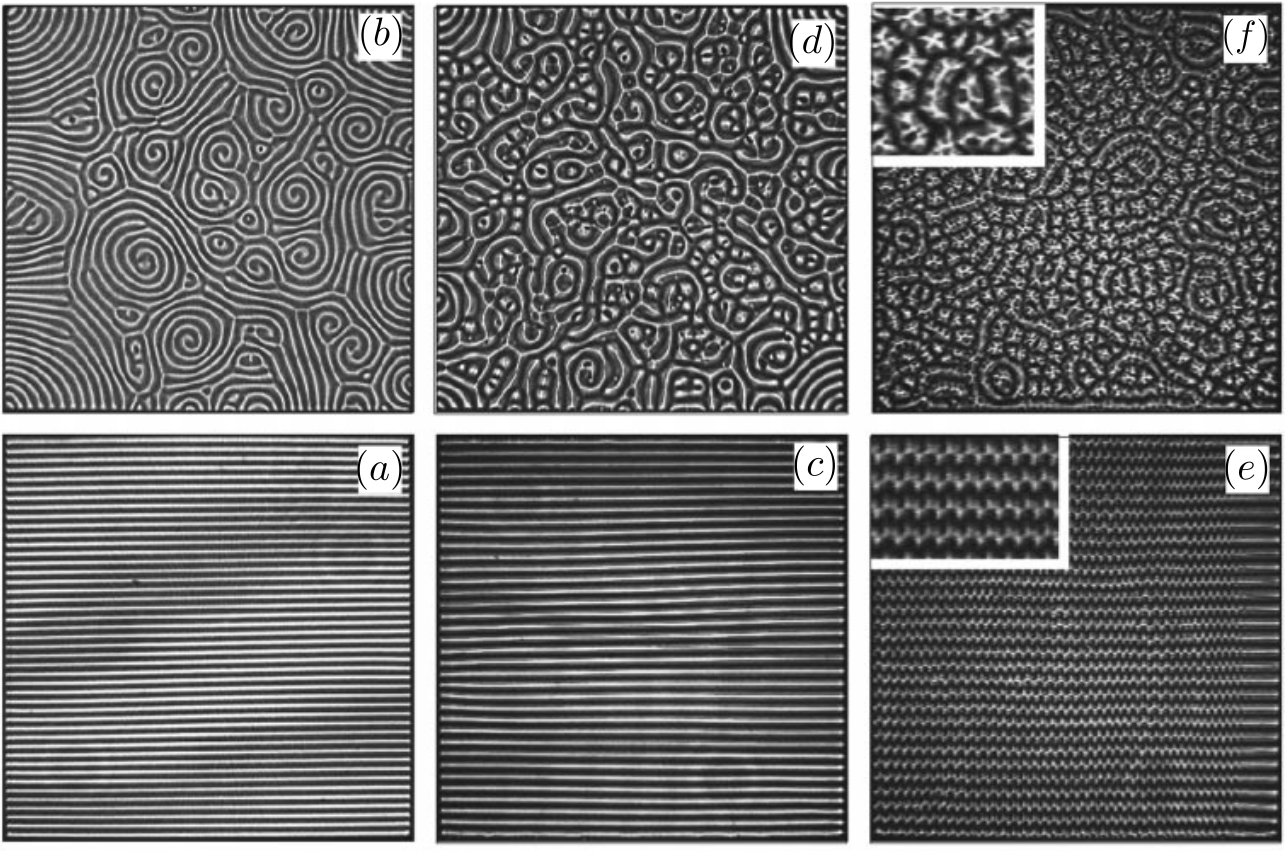
\includegraphics[width=0.8\textwidth]{Background/Figures/bistability.png}
    \caption{The coexistence of spiral defect chaos (SDC, top row) and ideal straight rolls (ISRs, bottom row) at (a,b) $Ra = 3279$, (c,d) $Ra = 6832$ and (e,f) $Ra = 10384$. The domain size is $\Gamma = 50$ and $Pr = 1$, adapted from \protect\DIFdelbeginFL \DIFdelFL{\mbox{%DIFAUXCMD
\cite{cakmur_bistability_1997}}\hspace{0pt}%DIFAUXCMD
}\DIFdelendFL \DIFaddbeginFL \DIFaddFL{\mbox{%DIFAUXCMD
\citet{cakmur_bistability_1997}}\hspace{0pt}%DIFAUXCMD
}\DIFaddendFL .}
    \label{fig:sdc_isr}
\end{figure}
%DIF <  The existence of multiple stable states apart from ISRs suggest that RBC forms a multiple bistable systate above $Ra_c$.
%DIF <  To compliate matter further, an instrinsic chaotic state of convection was discovered.

% SDC
In the \DIFdelbegin \DIFdel{late }\DIFdelend 1990s, convection rolls exhibiting spatio-temporal chaotic behaviour known as spiral defect chaos (SDC) were observed within the same stability boundaries where ISRs were expected \citep{morris_spiral_1993, hu_convection_1993,decker_spiral_1994,hu_convection_1995,morris_spatio-temporal_1996,cakmur_bistability_1997,ahlers_experiments_nodate,egolf_importance_1998,egolf_mechanisms_2000,chiam_mean_2003,vitral_spiral_2020}.
Notably, ISRs emerge with carefully prepared initial conditions\DIFaddbegin \DIFadd{, }\DIFaddend while uncontrolled initial conditions lead to SDC.
It is now well established that SDC exists as \DIFaddbegin \DIFadd{an }\DIFaddend intrinsic attractor of RBC, independent of sidewall conditions \DIFdelbegin \DIFdel{\mbox{%DIFAUXCMD
\cite{morris_spatio-temporal_1996}}\hspace{0pt}%DIFAUXCMD
}\DIFdelend \DIFaddbegin \DIFadd{\mbox{%DIFAUXCMD
\citet{morris_spatio-temporal_1996}}\hspace{0pt}%DIFAUXCMD
}\DIFaddend , forming a bistable system with ISRs \citep{cakmur_bistability_1997} across a range of $Ra$ at $Pr = 1$ illustrated in figure \ref{fig:sdc_isr}.
\DIFdelbegin \DIFdel{However, this bistability appears to be Prandtl number dependent. 
}\DIFdelend At $Pr = 4$, \DIFdelbegin \DIFdel{the }\DIFdelend SDC appears to be transient\DIFaddbegin \DIFadd{, }\DIFaddend decaying towards ISRs over long periods\DIFaddbegin \DIFadd{, suggesting that the bistable system is $Pr$ dependent }\DIFaddend \citep{bajaj_competition_1997}.
SDC has also been replicated in numerical simulations using two-dimensional Swift-Hohenberg equations \citep{swift_hydrodynamic_1977,xi_spiral_1993,xi_spatiotemporal_1995,schmitz_spiral-defect_2002,karimi_exploring_2011}.
The critical Rayleigh number for the onset of SDC, $Ra_s$, depends on the domain's aspect ratio, and Prandtl number \citep{hu_convection_1995,bajaj_competition_1997,cakmur_transition_1997,bodenschatz_recent_2000}.
% Investigations into quantifying the onset of SDC in terms of Rayleigh number remain inconclusive as it appears to depend on the domain's aspect ratio, and Prandtl number \citep{hu_convection_1995,bajaj_competition_1997,cakmur_transition_1997,bodenschatz_recent_2000}.
%DIF <  The critical reduced Rayleigh number for the onset of SDC, $\varepsilon_s$, has been observed to decrease with increasing $\Gamma$, and increase with increasing $Pr$ \cite{hu1995a, hu1995b, bajaj1997, Cakmur97, bodenschatz2000}.
%DIF >  The critical reduced Rayleigh number for the onset of SDC, $\varepsilon_s$, has been observed to decrease with increasing $\Gamma$, and increase with increasing $Pr$ \citet{hu1995a, hu1995b, bajaj1997, Cakmur97, bodenschatz2000}.
SDC has been primarily reported in large aspect ratio domains ($\Gamma \gtrsim 20$), suggesting \DIFaddbegin \DIFadd{that }\DIFaddend a minimal domain size \DIFaddbegin \DIFadd{is required }\DIFaddend for SDC to occur \citep{bodenschatz_recent_2000}.
This is consistent with the leading Lyapunov exponents of SDC\DIFdelbegin \DIFdel{which becomes smaller with decreasing }\DIFdelend \DIFaddbegin \DIFadd{, which increases with }\DIFaddend $\Gamma$ \citep{egolf_mechanisms_2000, paul_extensive_2007}.
To \DIFdelbegin \DIFdel{better }\DIFdelend characterise SDC, several studies have investigated its spatial-temporal properties, such as the averaged roll-curvature \DIFdelbegin \DIFdel{\mbox{%DIFAUXCMD
\cite{hu_convection_1995}}\hspace{0pt}%DIFAUXCMD
}\DIFdelend \DIFaddbegin \DIFadd{\mbox{%DIFAUXCMD
\citet{hu_convection_1995}}\hspace{0pt}%DIFAUXCMD
}\DIFaddend , probability distribution of spirals \DIFdelbegin \DIFdel{\mbox{%DIFAUXCMD
\cite{ecke_excitation_1995, liu_spiral-defect_1996} }\hspace{0pt}%DIFAUXCMD
}\DIFdelend \DIFaddbegin \DIFadd{\mbox{%DIFAUXCMD
\citep{ecke_excitation_1995, liu_spiral-defect_1996} }\hspace{0pt}%DIFAUXCMD
}\DIFaddend and correlation length-/time-scales \citep{morris_spiral_1993, morris_spatio-temporal_1996, cakmur_transition_1997}.
Specifically, the correlation length-scales were found to grow exponentially \DIFdelbegin \DIFdel{with }\DIFdelend \citep{morris_spiral_1993, morris_spatio-temporal_1996, cakmur_transition_1997}, suggesting that \DIFaddbegin \DIFadd{the }\DIFaddend transition from ISRs to SDC is related to phase transitions.
Similar \DIFdelbegin \DIFdel{`SDC-liked' has }\DIFdelend \DIFaddbegin \DIFadd{SDC-like patterns have }\DIFaddend been observed in \DIFdelbegin \DIFdel{other pattern-formation systems, including rotating RBC \mbox{%DIFAUXCMD
\cite{hu_convection_1997}}\hspace{0pt}%DIFAUXCMD
}\DIFdelend \DIFaddbegin \DIFadd{rotating RBC \mbox{%DIFAUXCMD
\citep{hu_convection_1997}}\hspace{0pt}%DIFAUXCMD
}\DIFaddend , dielectric barrier discharge \DIFdelbegin \DIFdel{\mbox{%DIFAUXCMD
\cite{dong_observation_2005} }\hspace{0pt}%DIFAUXCMD
}\DIFdelend \DIFaddbegin \DIFadd{\mbox{%DIFAUXCMD
\citep{dong_observation_2005} }\hspace{0pt}%DIFAUXCMD
}\DIFaddend and advection diffusion reaction systems \DIFdelbegin \DIFdel{\mbox{%DIFAUXCMD
\cite{affan_spiral_2014}}\hspace{0pt}%DIFAUXCMD
}\DIFdelend \DIFaddbegin \DIFadd{\mbox{%DIFAUXCMD
\citep{affan_spiral_2014}}\hspace{0pt}%DIFAUXCMD
}\DIFaddend .

%DIF <  Given the co-existence of ISRs and SDC in the parameter space of $\varepsilon$, it is known that they form bistability at $Pr \approx 1$ in a spatially extended domain, supported by experiments over a range of $\varepsilon(>0)$ \cite{Cakmur97}.
%DIF <  The chaotic state of SDC is unstable at $Pr=4$, where multiple spiral patterns coarsen into a single spiral, before evolving into straight-curved rolls over a long period \cite{bajaj1997}.
\DIFdelbegin %DIFDELCMD < 

%DIFDELCMD < %%%
%DIF <  For large aspect ratios, $\Gamma \gtrsim  20$, convection rolls can exhibit spatiotemporal chaotic behaviour, known as spiral defect chaos (SDC) within the same $Ra$ range \citep{Morris93,Decker94,hu1995b,morris1996,Cakmur97,ahlers1998,egolf1998,chiam2003,vitral2020}.
%DIF <  It is now established that both SDC and ISR can coexist at the same $Ra$, forming a bistable system confirmed experimentally \citep{Cakmur97}.
%DIFDELCMD < 

%DIFDELCMD < %%%
%DIF <  HYSTERSIS
%DIF <  Experimental investigations of RBC in moderate domain sizes ($\Gamma  = L/d \approx 14$ refers to the domain's aspect ratio) in rectangular (straight rolls) and cylinderical (concentric rolls) domains showed that the wavenumbers are confined within the Busse balloon.
%DIF <  Depending on $Pr$, either mechanism could arise, increasing the effective roll wavenumber of the stability to adhere within the stability boundaries of the Busse balloon.
%DIF <  For higher roll wavenumbers instabilities, the skewed-variose secondary instabilities arise, described by roll-pinching and merging where the effective roll-wavenumber is reduced to fall within the Busse balloon.
%DIF <  At higher $Ra$, the oscillatory (OS) instability appears for $Pr \lesssim 1$ while the knotted stability appear for higher $Pr$.
%DIF <  The oscillatory instability forms oscillatory ISRs reported by \cite{willis_oscillatory_1970}, while the knotted instability leads to spoke-liked covection patterns.
%DIF <  , the cross roll (CR),  zig-zag and the well known Eckhaus secondary instabilties emerge.
%DIF <  Lastly, the onset of a generic Eckhaus instability leads to either a roll destruction or emergence to stay within the Busse balloon.
%DIF <  We will focus the secondary instabilities at $Pr = 1$ in this thesis.
%DIFDELCMD < 

%DIFDELCMD < %%%
%DIF <  At $Pr \approx 1$, the secondary instabilities for large wavelengths are delimited by the cross-roll (CR) instability and the Eckhaus instability (not shown).
%DIF <  The CR instability generates an addition roll orthogonal to the existing roll which increasing the effect roll wavenumber.
%DIF <  Depending of the initial roll wavenumber, the Eckhaus instability either generates an additional or destroy rolls so that the stability boundaries are adhered to.
%DIF <  The secondary instabilities for small wavelengths are delimited by the skewed-varicosed instability, where adjacent rolls pinches and merge wher a new ISR emerge adhering to the stability boundaries.
%DIFDELCMD < 

%DIFDELCMD < %%%
%DIF <  For high Prandtl number fluids, the zig-zag instability occurs at small wavenumbers, causing wavy distortions.
%DIFDELCMD < 

%DIFDELCMD <  %%%
%DIF <  long-wavelength modulation instabilities, where the disturbance wavenumber $|\mathbf{s}| \ll |\mathbf{q}|$ perturbs the ISR pattern. Depending on the direction and structure of the perturbation, one observes different instability types: the Eckhaus instability (ECK), involving modulations of roll spacing with $\mathbf{s} \parallel \mathbf{q}$; the zig-zag instability (ZZ), characterised by undulations along the roll axis with $\mathbf{s} \perp \mathbf{q}$; and the more general skewed varicose instability (SV), which encompasses both. For Prandtl numbers near unity ($Pr \approx 1$), SV instabilities delineate the high-wavenumber ($q$) boundary of the Busse balloon.
%DIFDELCMD < 

%DIFDELCMD < %%%
%DIF <  In contrast, at low Prandtl numbers ($Pr \ll 1$), an oscillatory instability limits the stability region from above. This mode, marked by $\text{Im}(\omega(k)) \neq 0$ and $\mathbf{s} \approx \mathbf{q}$, leads to time-dependent behavior with propagating wave patterns and significant vertical vorticity. Additionally, short-wavelength instabilities can destabilize the ISR pattern through disturbances with $|\mathbf{s}| \approx |\mathbf{q}|$ but at a finite angle relative to $\mathbf{q}$. For $Pr \approx 1$, the cross-roll instability (CR) becomes prominent at small $q$, where new rolls form orthogonally to the original ones, preventing the development of overly short-wavelength patterns.
%DIFDELCMD < 

%DIFDELCMD < %%%
%DIF <  Despite the idealised assumptions underlying the Busse balloon, experiments \citep[see][]{egolf_dynamical_1998} have demonstrated that its stability boundaries remain locally applicable to patches of ISR even in more disordered or weakly turbulent regimes. As such, the Busse balloon remains a central tool in understanding the transition from regular convection patterns to spatiotemporal complexity in Rayleigh–Bénard convection.
%DIF <  Depending on the value of the Prandlt number, different types of secondary instabilities may arise, secondary instabilities may arise.
%DIF <  % The secondary instabilities of thermal convection rolls are crucial for understanding the transition to more complex flow patterns.
%DIF <  In low Prandtl number fluids, the oscillatory instability appears dominant, characterised by oscillations propagating along the ro, and the knot instability, a modification of the cross-roll instability that introduces a spoke pattern form of convectionlls.
%DIF <  For intermediate $Pr$, skewed varicose instability, causing in a merging of neighbour rolls elongating the wavelength of the rolls.
%DIF <  These instabilities, arising from different physical mechanisms related to momentum and heat transfer, dictate the stability and evolution of convection patterns as parameters like the Rayleigh and Prandtl numbers change.
%DIFDELCMD < 

%DIFDELCMD < %%%
%DIF <  It is noted that weakly nonlinear stability analysis is only limited to $Ra$ slight above $Ra_c$ \citep{busse_oscillatory_1972}.
%DIF <  As noted by \cite{busse_oscillatory_1972}, the applicability of weakly nonlinear analysis to slightly above onset, 
%DIF < which has been found to be a secondary instability of stationary convection rolls with complex eigenvalues.
%DIF <  The theoretical foundations of performing stability analysis using expansion in powers of amplitude  (\emph{weakly nonlinear analysis}) was considered by \cite{eckhaus_studies_1965}, in which he applied it to the problem of parallel shear flows.
%DIF <  The important contribution was that slightly above the onset, stable stationary rolls are found within the range of $Ra > Ra_c + 3\eta(\alpha - \alpha_c)^2$, where $\eta = \frac{1}{2}\frac{\partial Ra}{\partial \alpha}|_{Ra_c}$.
%DIF <  \cite{busse_instabilities_1971} then extended the same technique to Rayleigh-B\'{e}nard convection, in which $\eta$ was found to depend on $Pr$.
%DIFDELCMD < 

%DIFDELCMD < %%%
%DIF <  To complicate the subject further, ISRs appear to be an exception rather than the rule \citep{croquette_convective_1989-1} as multiple `non-ISR' states, in the form os squares, travelling/stationary targets, giant rotating spirals and oscillatory convection patterns have been found over the years \citep{croquette_convective_1989,croquette_convective_1989-1,plapp_dynamics_1998,hof_flow_1999,rudiger_pattern_2000,boronska_extreme_2010,boronska_extreme_2010-1}.
%DIF <  For example, investigations of cylinderical RBC in small aspect-ratio revealed eight stationary statesand two oscillatory states.
%DIF <  These findings were later supported by numerical experiments and bifurcation analyses.
%DIFDELCMD < 

%DIFDELCMD < %%%
%DIF <  \begin{enumerate}
%DIF <      \item Saturated States
%DIF <      \item Busse balloon for Pr = 1
%DIF <      \item Skew-varicose, Eckhaus, Cross-roll instabilities
%DIF <      \item Low $Pr$ and high $Pr$.
%DIF <      \item What happens above the Busse balloon?
%DIF <  \end{enumerate}
%DIF <  
%DIF <  \begin{enumerate}
%DIF <      \item Statisitical description of spatial-temporal chaos (i.e correlation length, time etc..)
%DIF <      \item Challenge with quantifying the onset
%DIF <  \end{enumerate}
%DIFDELCMD < 

%DIFDELCMD < %%%
%DIF <  \subsection{Turbulent Rayleigh Benard: ultimate regime vs classical regime
%DIF <  \begin{enumerate}
%DIF <      \item Onset of turbulence RBC
%DIF <      \item Introduce classical vs ultimate regime and scaling arguments of $Nu$.
%DIF <  \end{enumerate}
%DIFDELCMD < 

%DIFDELCMD < %%%
\DIFdelend %%%%%%%%%%%%%%%%%%%%%%%%%%%%%%%%%%
% Rayleigh Benard Poiseuille flows
%%%%%%%%%%%%%%%%%%%%%%%%%%%%%%%%%%

\section{Rayleigh-B\'{e}nard Poiseuille (RBP) flows}\label{sec:bkgrd_RBP}

%DIF <  The RBP system consist of the primary instabilities of the RBC and RBP configurations and in the limiting cases, we observe the onset of convection rolls at $Ra_c = 1708$, and Tollmien Schlicting waves at $Re = 5772$.
\begin{figure}[h]
    \centering
    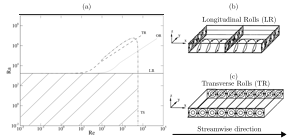
\includegraphics[width=\textwidth]{Background/Figures/RBP/RBP.pdf}
    \caption{(a) Neutral stability curves of longitudinal rolls (LR), oblique rolls (OR), transverse rolls (\DIFdelbeginFL \DIFdelFL{LR}\DIFdelendFL \DIFaddbeginFL \DIFaddFL{TR}\DIFaddendFL ) and Tollmien-Schlicting (TS) waves, adapted from \protect\DIFdelbeginFL \DIFdelFL{\mbox{%DIFAUXCMD
\cite{john_soundar_jerome_transient_2012}}\hspace{0pt}%DIFAUXCMD
}\DIFdelendFL \DIFaddbeginFL \DIFaddFL{\mbox{%DIFAUXCMD
\citet{john_soundar_jerome_transient_2012}}\hspace{0pt}%DIFAUXCMD
}\DIFaddendFL . The shaded area refers to \DIFdelbeginFL \DIFdelFL{damped perturbations}\DIFdelendFL \DIFaddbeginFL \DIFaddFL{a linearly stable region}\DIFaddendFL . Sketch of (b) longitudinal and (c) transverse rolls, adapted from \protect\DIFdelbeginFL \DIFdelFL{\mbox{%DIFAUXCMD
\cite{kelly_onset_1994}}\hspace{0pt}%DIFAUXCMD
}\DIFdelendFL \DIFaddbeginFL \DIFaddFL{\mbox{%DIFAUXCMD
\citet{kelly_onset_1994}}\hspace{0pt}%DIFAUXCMD
}\DIFaddendFL .}
    \label{fig:primary_instabilities}
\end{figure}
This section describes the developments of Rayleigh-B\'{e}nard Poiseuille (RBP) flows, integrating key findings from both plane Poiseuille flow (PPF) and Rayleigh-B\'{e}nard convection (RBC) systems discussed in \S \ref{sec:bkgrd_transitional} and \S \ref{sec:bkgrd_RBC} respectively.
The neutral stability curves in the Rayleigh-B\'{e}nard Poiseuille (RBP)\DIFdelbegin \DIFdel{comprising of both plane Poisueuille }\DIFdelend \DIFaddbegin \DIFadd{, comprising both plane Poiseuille }\DIFaddend flow (PPF) and Rayleigh-B\'{e}\DIFdelbegin \DIFdel{anrd }\DIFdelend \DIFaddbegin \DIFadd{nard }\DIFaddend convection (RBC) systems, are bounded by the onset of Tollmien-Schlicting waves at $Re_{c} = 5772.22$ \citep{orszag_accurate_1971}, and by the onset of convection rolls at $Ra_c = 1708$ \citep{pellew_maintained_1940}, respectively.
%DIF <  In RBP systems, the imposed mean Poiseuille flow in the RBP system breaks the rotational symmetry of the convection rolls, categorising them based on their orientation to the mean flow direction, namely: longitudinal ($\alpha= 0, \beta \neq 0$), transverse ($\alpha \neq 0, \beta = 0$) and oblique rolls ($\alpha \neq 0, \beta \neq 0$).
In RBP systems, the imposed mean Poiseuille flow in the RBP system breaks the rotational symmetry of the convection rolls, categorising them based on their orientation to the mean flow direction, namely: longitudinal, transverse and oblique rolls.
%DIF <  Due to the imposed mean flow, the convection rolls are not rotationally invariant, and their orientation with respect to the mean matters.
%DIF <  Generally, convection rolls that are aligned, diagonal and perpendicular to the mean flow are referred to longitudinal, oblique and transverse rolls.
These primary instabilities were first investigated by \DIFdelbegin \DIFdel{\mbox{%DIFAUXCMD
\cite{gage_stability_1968} }\hspace{0pt}%DIFAUXCMD
}\DIFdelend \DIFaddbegin \DIFadd{\mbox{%DIFAUXCMD
\citet{gage_stability_1968} }\hspace{0pt}%DIFAUXCMD
}\DIFaddend in an infinitely extended layer.
For longitudinal rolls, the linearised system reduces to the classical RBC problem.
Thus, the critical Rayleigh number remains unchanged at $Ra_{\parallel} = Ra_{c} = 1708.8$ with a critical wavenumber, $\alpha_{\parallel} = \alpha_{c} = 3.13$, independent of Reynolds number and Prandtl number \citep{pellew_maintained_1940, kelly_onset_1994}.
In contrast, the critical Rayleigh number for the onset of transverse rolls increases with $Re$, and is also dependent on $Pr$ \citep{gage_stability_1968, muller_transversal_1992, nicolas_two-dimensional_1997}.
The critical Rayleigh number for the onset of \DIFdelbegin \DIFdel{obliqued rolls can derived using by applying a Squire}\DIFdelend \DIFaddbegin \DIFadd{oblique rolls can be obtained by applying Squire's }\DIFaddend transformation \citep{squire_stability_1933} to \DIFaddbegin \DIFadd{the }\DIFaddend transverse roll system.
For a given $Ra$, the corresponding critical $Re$ for the onset of oblique rolls is higher than that for transverse rolls \citep{gage_stability_1968}.
%DIF <  The critical Rayleigh number for the onset of obliqued rolls are obtained by performing a Squire transformation on the linearised transverse roll system where for a given $Ra$, the critical $Re$ of oblique rolls is higher than the critical $Re$ for transverse rolls \citep{gage_stability_1968}.
The neutral stability curves for the three different rolls are illustrated in figure \ref{fig:primary_instabilities}.
%DIF <  The neutral stability curves associated with the transverse rolls (TR), oblique rolls (OR) and longitudinal rolls (LR) are shown in figure \ref{fig:primary_instabilities}.
\DIFaddbegin \DIFadd{We note that we will use different definitions for $x,y,z$ in chapter \S \ref{chap:3} and \S \ref{chap:4}.
}\DIFaddend 

Experimental studies in channels with large transverse aspect ratios (i.e. span-to-depth) showed the onset of longitudinal rolls \citep{akiyama_experiments_1971,ostrach_heat_1975,fukui_longitudinal_1983}, while transverse rolls are more prevalent in narrower channels \citep{luijkx_existence_1981,ouazzani_etude_1989,ouazzani_etude_1990}.
Linear stability analysis of longitudinal rolls for finite channels confirms that $Ra_\parallel$ remains fairly independent for transverse aspect ratios greater than five, and increases quickly below that.
Hence, for small $Re$, \DIFaddbegin \DIFadd{the }\DIFaddend critical Rayleigh number of transverse rolls is smaller than that of longitudinal rolls, $Ra_\perp < Ra_\parallel$, giving rise to transverse rolls \citep{nicolas_linear_2000}.
%DIF <  , $Ra_\perp$,  $Ra_\parallel$ in narrow channels for small Reynolds numbers \citep{nicolas_linear_2000}, providing support for the preference of transverse rolls in narrow channels.
%DIF <  Indeed, linear stability analysis of narrow channel reveal that the $Ra_{\parallel}$ are increased relative to the $Ra_\perp$ for small $Re$ \citep{nicolas_linear_2000}.
%DIF <  \st{However, temporal linear stability analysis could not explain the observations by} \cite{ouazzani_etude_1990}\st{, where the laminar Poiseuille flow persisted in the same parameter space where transverse rolls were expected.}
However, laminar Poiseuille flow \DIFdelbegin \DIFdel{where }\DIFdelend \DIFaddbegin \DIFadd{was }\DIFaddend observed in the same parameter space where transverse rolls were expected from linear stability analysis \DIFdelbegin \DIFdel{\mbox{%DIFAUXCMD
\cite{ouazzani_etude_1989}}\hspace{0pt}%DIFAUXCMD
.
%DIF <  where reported laminar Poiseuille flow in the $Ra, Re$ parameter space where transverse rolls are expected based on temporal linear stability analysis.
%DIF <  However, linear temporal stability analysis failed to explain the experimental results from \cite{ouazzani_etude_1990}, where a laminar Poiseuille is observed in the parameter space where transverse rolls are expected.
}\DIFdelend \DIFaddbegin \DIFadd{\mbox{%DIFAUXCMD
\citet{ouazzani_etude_1989}}\hspace{0pt}%DIFAUXCMD
.
}\DIFaddend This discrepancy was resolved by \DIFdelbegin \DIFdel{\mbox{%DIFAUXCMD
\cite{muller_transversal_1992}}\hspace{0pt}%DIFAUXCMD
}\DIFdelend \DIFaddbegin \DIFadd{\mbox{%DIFAUXCMD
\citet{muller_transversal_1992}}\hspace{0pt}%DIFAUXCMD
}\DIFaddend , who showed that transverse rolls may be convectively or absolutely unstable, with the transition boundary corroborating with experimental data.
Later, \DIFdelbegin \DIFdel{\mbox{%DIFAUXCMD
\cite{carriere_convective_1999} }\hspace{0pt}%DIFAUXCMD
showed that }\DIFdelend \DIFaddbegin \DIFadd{\mbox{%DIFAUXCMD
\citet{carriere_convective_1999} }\hspace{0pt}%DIFAUXCMD
}\DIFaddend demonstrated that longitudinal rolls are always convectively unstable.
%DIF <  can be either convectively or absolutely unstable, and the boundary between them matches with the experimental results of \cite{ouazzani_etude_1990}.
%DIF <  By considering the response from three-dimensional impulse, \cite{carriere_convective_1999} further demostrated that the longitudinal rolls, unlike the transverse rolls, are always convectively unstable.
%DIF <  The critical Rayleigh number for oblique and transverse rolls matches that of RBC at $Re=0$ due to horizontal isotropy, but increases as $Re$ increases, depending on $Pr$, i.e., $Ra_{\perp} = f(Re,Pr)
Nonmodal stability analysis of subcritical RBP by \DIFdelbegin \DIFdel{\mbox{%DIFAUXCMD
\cite{john_soundar_jerome_transient_2012} }\hspace{0pt}%DIFAUXCMD
}\DIFdelend \DIFaddbegin \DIFadd{\mbox{%DIFAUXCMD
\citet{john_soundar_jerome_transient_2012} }\hspace{0pt}%DIFAUXCMD
}\DIFaddend revealed that the optimal transient growth is primarily \DIFdelbegin \DIFdel{dominanted }\DIFdelend \DIFaddbegin \DIFadd{dominated }\DIFaddend by streamwise rollers similar to those of PPF \citep{reddy_energy_1993}, with a spanwise wavenumber of $\beta_{opt} \approx 2.05$.
The maximum \DIFdelbegin \DIFdel{amplifcation }\DIFdelend \DIFaddbegin \DIFadd{amplification }\DIFaddend factor, $G_{max}$\DIFaddbegin \DIFadd{, }\DIFaddend increases modestly with $Ra$, and the critical wavenumber approaches $\alpha_{\parallel}$, indicative of longitudinal rolls.
%DIF <  Nonmodal stability analyses of subcritical RBP indicate that the optimal transient growth $G_{max}$ increases gradually with $Ra$.
%DIF <  The wavenumber of the optimal initial conditions, $\beta_{max}$, resembles that observed in shear flows \citep{reddy_energy_1993}, and gradually approaches the critical wavenumber of convection rolls, $\alpha_{\parallel}$, as $Ra$ increases \citep{john_soundar_jerome_transient_2012}.
%DIF <  For $Re > 0$, the longitudinal rolls appear as the dominant primary instability \citep{gage_stability_1968}.
%DIF <  Since longitudinal rolls are the dominant primary instability for $Re > 0$ in infinite domains, their secondary stability have been analysed by \cite{clever_instabilities_1991}.

For $Re > 0$ in infinite domains, the longitudinal rolls emerge as the dominant primary instability \citep{gage_stability_1968}, and their secondary stability was analysed by \DIFdelbegin \DIFdel{\mbox{%DIFAUXCMD
\cite{clever_instabilities_1991}}\hspace{0pt}%DIFAUXCMD
}\DIFdelend \DIFaddbegin \DIFadd{\mbox{%DIFAUXCMD
\citet{clever_instabilities_1991}}\hspace{0pt}%DIFAUXCMD
}\DIFaddend .
They identified a time-dependent, wavy instability near $Re \sim 100$, giving rise to tertiary solutions in the form of wavy rolls.
These wavy rolls have been observed experimentally and were found to be convectively unstable \citep{pabiou_observations_2003, pabiou_wavy_2005, nicolas_characterisation_2010}.
\DIFdelbegin \DIFdel{\mbox{%DIFAUXCMD
\cite{clever_instabilities_1991} }\hspace{0pt}%DIFAUXCMD
}\DIFdelend \DIFaddbegin \DIFadd{\mbox{%DIFAUXCMD
\citet{clever_instabilities_1991} }\hspace{0pt}%DIFAUXCMD
}\DIFaddend also hypothesised that the wavy rolls are less efficient at transporting \DIFdelbegin \DIFdel{heating }\DIFdelend \DIFaddbegin \DIFadd{heat }\DIFaddend than longitudinal rolls for the same $Ra$, which was later confirmed numerically by \DIFdelbegin \DIFdel{\mbox{%DIFAUXCMD
\cite{nicolas_influence_2012}}\hspace{0pt}%DIFAUXCMD
}\DIFdelend \DIFaddbegin \DIFadd{\mbox{%DIFAUXCMD
\citet{nicolas_influence_2012}}\hspace{0pt}%DIFAUXCMD
}\DIFaddend .
The influence of finite transverse aspect ratios on the onset of wavy rolls have also been studied \citep{xin_stability_2006, nicolas_characterisation_2010}, where the critical $Ra$ was found to be approximately 1.5 times higher than in infinite domains \DIFdelbegin \DIFdel{\mbox{%DIFAUXCMD
\cite{clever_instabilities_1991}}\hspace{0pt}%DIFAUXCMD
}\DIFdelend \DIFaddbegin \DIFadd{\mbox{%DIFAUXCMD
\citet{clever_instabilities_1991}}\hspace{0pt}%DIFAUXCMD
}\DIFaddend .
Furthermore, the effect of external excitation has been explored, showing that increased excitation amplitude can reduce the development length required for the formation of wavy roll \citep{nicolas_characterisation_2010,nicolas_influence_2012}.
In the turbulent regime, \DIFdelbegin \DIFdel{shear driven }\DIFdelend \DIFaddbegin \DIFadd{shear-driven }\DIFaddend turbulence has been shown to enhance heat transport in RBP flows \citep{scagliarini_heat_2014, scagliarini_law_2015, pirozzoli_mixed_2017}.
%DIF <  In finite streamwise extensions of RBP flows, the onset of convection rolls and the heat flux variations due to entrance effects have been investigated \citep{mahaney_effect_1988,lee_effect_1991,nonino_laminar_1991}.
Extensions of the RBP configuration, such as flows over wavy walls or with sinusoidal thermal forcing\DIFaddbegin \DIFadd{, }\DIFaddend have been investigated, potentially offering a reduction in drag and enhancing heat transport \citep{hossain_drag_2012,hossain_drag_2016,hossain_role_2020}.
%DIF <  RBP flows with sinusoidal heating and wavy walls have also been studied \citep{hossain_spectral_2021}.
For a comprehensive overview of RBP flows, the reader is referred to the reviews by \DIFdelbegin \DIFdel{\mbox{%DIFAUXCMD
\cite{kelly_onset_1994} }\hspace{0pt}%DIFAUXCMD
and \mbox{%DIFAUXCMD
\cite{nicolas_revue_2002}}\hspace{0pt}%DIFAUXCMD
}\DIFdelend \DIFaddbegin \DIFadd{\mbox{%DIFAUXCMD
\citet{kelly_onset_1994} }\hspace{0pt}%DIFAUXCMD
and \mbox{%DIFAUXCMD
\citet{nicolas_revue_2002}}\hspace{0pt}%DIFAUXCMD
}\DIFaddend .

%%%%%%%%%%%%%%%%
%DIF <  THESIS OUTLINE
%DIF >  SCOPE OF STUDY
%%%%%%%%%%%%%%%%
\DIFaddbegin \section{\DIFadd{Thesis objectives}}\label{sec:bkgrd_objs}
\DIFadd{While significant progress has been made in understanding the transition processes of Rayleigh-B\'{e}nard convection (see \S \ref{sec:bkgrd_RBC}) and plane Poiseuille flows (see \S \ref{sec:bkgrd_transitional}) independently, their combined interaction beyond primary linear instabilities (see \S \ref{sec:bkgrd_RBP}) remains largely unexplored.
In particular, the interaction between buoyancy-driven convection and shear-driven instability in Rayleigh-B\'{e}nard-Poiseuille (RBP) flow raises questions about transition mechanisms that may not be inferred from either system in isolation.
}\DIFaddend 

\DIFdelbegin \section{\DIFdel{Thesis Outline}}%DIFAUXCMD
\addtocounter{section}{-1}%DIFAUXCMD
%DIFDELCMD < \label{sec:bkgrd_thesis_outline}
%DIFDELCMD < 

%DIFDELCMD < %%%
%DIF <  The governing equations of the fluid motion in given by the Navier-Stokes equations with Boussinessq approximations,
%DIF <  \begin{equation}
%DIF <      \frac{\partial \mathbf{u}}{\partial t} + (\mathbf{u} \cdot \nabla) \mathbf{u} = -\frac{1}{\rho} \nabla p + \nu \nabla^2 \mathbf{u} + g\beta(T-T_0).
%DIF <  \end{equation}`
%DIF <  \begin{equation}
%DIF <      \frac{\partial T}{\partial t} + (\mathbf{u} \cdot \nabla)T = \kappa \nabla^2 T,
%DIF <  \end{equation}
%DIF <  \begin{equation}
%DIF <      \nabla  \cdot \mathbf{u} = 0.
%DIF <  \end{equation}
%DIF <  with arbitrary Dirichlet and Neumann boundary conditions.
%DIF <  \begin{equation}
%DIF <      \mathbf{u}_d, p_d, T_d \in \Omega_d, \quad \nabla\mathbf{u}_N, p_N, T_N \in \partial\Omega_N.
%DIF <  \end{equation}
%DIF <  where $\mathbf{u}, T, p$ refers to the velocity, temperature and pressure fields, primitive variables that are not known a priori and $\rho, \nu, \kappa$ refers to the properties of the fluid, namely, density, kinematic viscosity and thermal diffusivity.
%DIF <  For a given set of fluid properties $\rho, \nu, \kappa$ and geometric properties $L^*, t^*, u^*$ referring to an arbitrary length-, time- and velocity-scale, we are primarily interested in the behaviour of the fluid i.e if its laminar or turbulent.
%DIF <  In other words, we have a six control parameters that describes a fluid flow of interest.
%DIF <  To reduce the number of control parameters, we can suitably nondimensionalise the primitive variables by a velocity scale $u_c$, length scale, $L_x$, and time scale $u_c/L_x$, where $u_c$ refers to the centreline velocity of a laminar flow and $L_x$ refers to the streamwise length of the domain.
%DIF <  The nondimensional equations with Boussienessq approximations are now given as,
%DIF <  \begin{equation}
%DIF <      \frac{\partial \mathbf{u}}{\partial t} + (\mathbf{u}\cdot\nabla)\mathbf{u} = -\nabla p + \frac{1}{Re}\nabla^2 \mathbf{u} + \frac{Ra}{Re^2Pr} \theta
%DIF <  \end{equation}
%DIF <  \begin{equation}
%DIF <      \frac{\partial \theta}{\partial t} + (\mathbf{u} \cdot \nabla)\theta = \frac{1}{RePr}\nabla^2 \theta,
%DIF <  \end{equation}
%DIF <  \begin{equation}
%DIF <      \nabla \cdot \mathbf{u} = 0.
%DIF <  \end{equation}
%DIF <  where $\mathbf{u}, \theta, p$ refers to the nondimensionalised velocity, temperature and presure.
\DIFdelend In this thesis, \DIFdelbegin \DIFdel{I }\DIFdelend \DIFaddbegin \DIFadd{we }\DIFaddend focus on the transitional behaviour of \DIFdelbegin \DIFdel{fluid flowin Rayleigh-B\'{e}nard Poiseuille systems by conducting }\DIFdelend \DIFaddbegin \DIFadd{RBP flow, using }\DIFaddend direct numerical simulations and linear stability analysis.
%DIF <  addressing questions related to the onset of instabilities due to shear and buoyancy, and the (possible) competitive between shear and buoyancy driven instabilities.
Notably, the onset of instabilities does not necessarily lead to \DIFdelbegin \DIFdel{turbulence and may give rise to }\DIFdelend \DIFaddbegin \DIFadd{fully developed turbulence.
Instead, the system may exhibit }\DIFaddend flow regimes that are neither \DIFdelbegin \DIFdel{fully }\DIFdelend \DIFaddbegin \DIFadd{purely }\DIFaddend laminar nor fully turbulent.
For clarity, we \DIFdelbegin \DIFdel{refer to these flow regimes collectively as the transitional regime.
%DIF <  I would like to preface that while this thesis is dealing with onset of instabilities, it does not clearly indicate that the onset of such instabilities necessarily lead to turbulence, hence, for terminology sake, we shall be looking into transitional regimes where the fluid neither laminar nor turbulent.
}\DIFdelend \DIFaddbegin \DIFadd{collectively refer to such intermediate states as the }\textit{\DIFadd{transitional regime}}\DIFadd{.
}\DIFaddend 

\DIFdelbegin \DIFdel{While significant progress has been made in understanding the transition process of Rayleigh-B\'{e}nard convection and plane Poiseuille flows separately, their combined effects remains largely unexplored.
%DIF <  There had been significant progress in our understanding of the instabilities of Rayleigh-B\'{e}nard convection and plane Poiseuille flows, their combined effects are not known.
For instance, do }\DIFdelend \DIFaddbegin \DIFadd{Through a combination of exploratory DBS and linear stability analysis, this work aims to address the following questions:
}\begin{enumerate}
    \item \DIFadd{Do }\DIFaddend convection rolls promote the transition to \DIFdelbegin \DIFdel{shear driven turbulence?
    And conversely, how does shear affect }\DIFdelend \DIFaddbegin \DIFadd{shear-driven turbulence?
    }\item \DIFadd{How does shear influence }\DIFaddend the bistable dynamics between ideal straight rolls (ISRs) and spiral defect chaos (SDC)?
\DIFaddbegin \end{enumerate}
\DIFaddend These questions are \DIFdelbegin \DIFdel{explore }\DIFdelend \DIFaddbegin \DIFadd{examined }\DIFaddend in \S \ref{chap:3}.
\DIFaddbegin \DIFadd{The answers to these questions may have implications for enhancing microprocessing chip-cooling technologies and improving thin-film fabrication using chemical vapour deposition processes (see \S \ref{sec:bkgrd_overview}).
}\DIFaddend 

\DIFaddbegin \DIFadd{In \S \ref{chap:4}, we adopt a dynamical systems perspective to study the bistability between ISRs and SDC in Rayleigh-B\'{e}nard convection.
}\DIFaddend Although the co-existence of ISRs and SDC as bistable states \DIFdelbegin \DIFdel{in Rayleigh-B\'{e}nard convection }\DIFdelend is well established, the \DIFdelbegin \DIFdel{existence of multiple }\DIFdelend \DIFaddbegin \DIFadd{presence of multiple stable }\DIFaddend states raises further questions about the \DIFdelbegin \DIFdel{notion of bistability.
In \S \ref{chap:4}, we investigate the }\DIFdelend \DIFaddbegin \DIFadd{underlying state-space structure.
We examine this }\DIFaddend state-space structure \DIFdelbegin \DIFdel{underlying ISRs and SDC, identifying }\DIFdelend \DIFaddbegin \DIFadd{and identify }\DIFaddend several stable invariant solutions referred to as \textit{elementary \DIFdelbegin %DIFDELCMD < \MBLOCKRIGHTBRACE %%%
\DIFdelend states\DIFaddbegin } \DIFaddend that underpin the pattern formation of SDC.
%DIF <  We explore the state space structure of ideal straight rolls (ISRs) and spiral defect chaos (SDC) in \S \ref{chap:4}, identifying several stable invariant states referred to as \textit{elementary} states, underpinning the pattern formation of SDC.
%DIF <  Subsequently, we explore the state space structure of the bistable system between ISRs and SDC in \S \ref{chap:4}.
%DIF <  \begin{enumerate}
%DIF <  \item From an academia point of view, the 
%DIF <  Within academia, the onset and transition to turbulence in Rayleigh-B\'{e}nard Poiseuille flows remains poorly understand.
%DIF <  
%DIF <  \end{enumerate}
\DIFaddbegin \DIFadd{This analysis provides a state-space interpretation of the bistable system between ISRs and SDC.
}\DIFaddend 

\DIFdelbegin \DIFdel{The thesis is structured into the }\DIFdelend %DIF > %%%%%%%%%%%%%%%
%DIF >  THESIS OUTLINE
%DIF > %%%%%%%%%%%%%%%
\DIFaddbegin 

\section{\DIFadd{Thesis outline}}\label{sec:bkgrd_outline}
\DIFadd{This thesis consists of five chapters and is organised as }\DIFaddend follows: 
\begin{enumerate}

    \item \S \ref{chap:1} provides the introduction and a review of relevant literature.
    \item \S \ref{chap:2} presents the numerical methods, including the spectral/\textit{hp} element method, algorithms for solving the Navier-Stokes equations, linear stability analysis and edge tracking.
    \item \S \ref{chap:3} introduces the $Ra-Re$ phase space of RBP flows, with a particular focus on the role of longitudinal rolls in sustaining turbulence. We introduce the \textit{thermally-assisted sustaining process} - an alternative route towards turbulence via linearly unstable longitudinal rolls
    \item \S \ref{chap:4} explores the organisation of the state space of spiral defect chaos and ideal straight rolls $Ra = 2903$, accompanied by \textit{elementary} states, edge states and \DIFdelbegin \DIFdel{highlight }\DIFdelend \DIFaddbegin \DIFadd{highlights }\DIFaddend some pathways towards SDC\DIFaddbegin \DIFadd{.
    }\DIFaddend \item Finally, \S \ref{chap:5} \DIFdelbegin \DIFdel{conludes }\DIFdelend \DIFaddbegin \DIFadd{concludes }\DIFaddend this thesis and suggests possible avenues of future research.
\end{enumerate}
\DIFdelbegin \DIFdel{.
}%DIFDELCMD < 

%DIFDELCMD < %%%
%DIF <  \begin{enumerate}
%DIF <     \item Academic motivation - flow structures, statistics, transition.
%DIF <     \item Application motivation - shear, heat transfer. Chip cooling, thin-film fabrication and atmospheric boundary layer.
%DIF <  \end{enumerate}
%DIF <  We seek to investigate the influence of unstable stratification quantified by Rayleigh number $Ra$, on the behaviour tuburlent-laminar bands. 
%DIF <  The onset of convection occurs at a critical Rayleigh number of $Ra_c > 1708$, in the form of a pair of convection rolls.
%DIF <  When aligned in the streamwise direction, the convection rolls are seemingly analogous to a pair of counter-rotating vortices, an optimal initial condition for transient growth. 
%DIF <  Our investigation naturally answers a few questions related to turbulent-laminar bands.
%DIF <  For example, does the onset of turbulent-laminar bands, $Re_{cr}$ decrease with increasing $Ra$?
%DIF <  Do $Ra$-effects influence the structure of turbulent-laminar bands i.e band angle/width? 
%DIF <  
%DIF <  The answers to our research will have important implications Rayleigh-B\'{e}nard Poiseuille flows, ubiquitous in atmospheric, geophysical and engineering flows.
\DIFdelend 

    \chapter{Numerical Methods}\label{chap:2}
In this chapter, we will discuss the fundamentals of numerical methods relevant for solving the Navier-Stokes equations.
We begin the discussion of the method \DIFdelbegin \DIFdel{weighted of }\DIFdelend \DIFaddbegin \DIFadd{of weighted }\DIFaddend residuals (\S \ref{sec:methodofweightedresiduals}) and the spatial discretisation using spectral/\emph{hp} element methods in one dimension (\S \ref{sec:spectralhpelementmethods}).
This is followed by techniques for solving the Navier-Stokes equations (\S \ref{sec:numeraltechniquesforNS}), such as the velocity-correction scheme, enforcing a constant flow rate and the quasi-3D approach for semi-homogeneous domains. 
This chapter concludes with numerical techniques for performing stability analysis of the Navier-Stokes equations (\S \ref{sec:stabilityanalysisofNS}), including eigenvalue computation and edge tracking.
%DIF <  In this chapter, I will present the numerical methods ultilised in this thesis.
%DIF <  The premise of numerical methods is to solve for the the partial differential equations, the Navier-Stokes equations.
%DIF <  The incompressible Navier-Stokes equations describe the time- and spatial-varying velocity field and pressure field.
%DIF <  One of the foundations of solving partial differential equations begin with the method of weighted residuals. 

%%%%%%%%%%%%%%%%%%%%%%%%%%%%%%%%%%
% 3.1 METHOD OF WEIGHTED RESIDUALS
%%%%%%%%%%%%%%%%%%%%%%%%%%%%%%%%%%

\section{Method of weighted residuals}\label{sec:methodofweightedresiduals}
Spatial discretisation errors, or residuals, arise as one seeks an approximate solution \DIFdelbegin \DIFdel{to some }\DIFdelend \DIFaddbegin \DIFadd{of a }\DIFaddend partial differential equation (PDE).
The method of weighted residuals provides a \DIFdelbegin \DIFdel{generic }\DIFdelend \DIFaddbegin \DIFadd{general }\DIFaddend mathematical framework in which constraints on the residual \DIFdelbegin \DIFdel{could }\DIFdelend \DIFaddbegin \DIFadd{can }\DIFaddend be applied flexibly, \DIFaddbegin \DIFadd{thereby }\DIFaddend defining the spatial discretisation scheme and its convergence properties.
We approximate the solution of PDE by considering a finite expansion of a suitable basis, to which its coefficients are sought \DIFdelbegin \DIFdel{after }\DIFdelend by minimising the inner product between the PDE and a test (or weight) function.
To demonstrate this, we consider a linear partial differential equation as
\DIFdelbegin \DIFdel{,
}\DIFdelend \begin{equation}\label{eq:linear_operator}
    \mathbf{L}[u(x)] = 0, \quad x \in \Omega,
\end{equation}
where $\mathbf{L}$ refers to a linear spatial differential operator subjected to some boundary conditions within the domain, $\Omega$, while $u(x)$ refers to the exact solution of $\mathbf{L}$.
Examples of PDEs with linear spatial differential operators include the Laplace equation, $\nabla^2 u = 0 $, \DIFaddbegin \DIFadd{the }\DIFaddend Poisson equation, $\nabla^2 u - f = 0$, and the Helmholtz equation, $\nabla^2 u - \lambda u  + f = 0$.
We suppose that the exact solution $u(x)$ can be approximated (discretised) by $N$ finite number of global basis (or expansion) functions, $\Phi(x)$\DIFdelbegin \DIFdel{.
}\DIFdelend \DIFaddbegin \DIFadd{:
}\DIFaddend \begin{equation}\label{eq:approximate}
    u(x) \approx u^\delta(x) = \sum_{i=0}^{N-1} \hat{u}_i \Phi_i(x),
\end{equation}
where $u^\delta(x)$ refers to the approximate solution of $u(x)$, consisting of a linear combination of the product between the $i^{th}$ basis coefficient, $\hat{u}_i$, and the $i^{th}$ global basis expansion, $\Phi_i(x)$, defined within $\Omega$.
Since $u^\delta(x)$ is an approximate solution of equation \eqref{eq:helmholtz}, we expect a residual (or error) between the exact solution, $u(x)$, and $u^\delta(x)$,
\begin{equation}\label{eq:residual}
    \mathbf{L}[u^\delta(x)] = R[u^\delta(x)],
\end{equation}
where $R[u^\delta(x)]$ refers to the residual which depends on the approximate solution $u^\delta(x)$ and varies within $\Omega$.
In other words, equation \eqref{eq:residual} might not be satisfied everywhere in $\Omega$. 
Next, we need to place restrictions on the residual, such that \DIFdelbegin \DIFdel{it }\DIFdelend the residual approaches zero, $R \rightarrow 0$, and the approximate solution approaches the exact solution, $u^\delta(x) \rightarrow u(x)$.
The method of weighted residuals places a restriction on the residual by applying an inner product between the governing equation \DIFdelbegin \DIFdel{, }\DIFdelend and $N$ test (or weight) functions, $v_j(x)$, and setting it to zero,
\begin{equation}\label{eq:weightinnerresidual}
    (v_j(x), R[u^\delta(x)]) = 0, \quad j = 0, ..., N-1.
\end{equation}
\begin{definition}[Inner product]
The inner product between two functions $f(x)$ and $g(x)$ is,
\begin{equation}
       (f, g) = \int_\Omega f(x) g(x) dx \nonumber.
\end{equation}
\end{definition}
%DIF <  where $(\, \cdot \, , \, \cdot \,)$ refers to an inner product, a measure of orthogonality between function $f(x)$ and $g(x)$ defined as,
%DIF <  \begin{equation}\label{eq:inner-product}
%DIF <         (f, g) = \int_\Omega f(x) g(x) dx.
%DIF <  \end{equation}
By enforcing equation \eqref{eq:weightinnerresidual}, the discrete problem becomes a system of $N$ ordinary differential equations to solve for the $N$ basis coefficients, $\hat{u}_i$.
The choice of test function defines the projection methods, and examples of different projection methods are shown in table \ref{tab:weightFunction}.
We emphasise that the method of weighted residuals only describes the projection method, but does not specify the type of basis expansions, as we will discuss later in \S \ref{sec:spectralhpelementmethods}.
The choice of projection method\DIFdelbegin \DIFdel{coupled with suitable basis expansionswill have different solution convergence properties }\DIFdelend \DIFaddbegin \DIFadd{, coupled with appropriate basis expansions, will yield different convergence properties of the solution}\DIFaddend .
Of particular interest is \DIFdelbegin \DIFdel{on }\DIFdelend how quickly the residual vanishes as the number of basis expansions increases.
For instance, by considering the Galerkin method coupled with Fourier expansions, one can expect exponential convergence for a sufficiently smooth problem\DIFaddbegin \DIFadd{, }\DIFaddend which is desirable for an efficient representation of turbulent dynamics.
%DIF <  Certain mathematical properties such as spectral convergence as desired in the case of Galerkin projection using Fourier expansions, 
%DIF <  The choice of \emph{trial} functions used in \emph{nektar++} will be elaborated in Section \ref{sec:modifiedBasis}.
%DIF <  the method of weighted residuals is only restrictive to the weight
%DIF <  Table \ref{tab:weightFunction} shows the different forms of weight functions and its corresponding numerical method.
\renewcommand{\arraystretch}{1.5} % Default value: 1
\begin{table}[h]
    \centering
        \begin{tabular}{cc}
            Weight functions & Projection method \\
            \hline
            $v_j(x) = \delta(x-x_j)$ & Collocation \\
            $v_j(x) =\left\{\begin{array}{ll}
                1 & \mbox{if } x \in \Omega_j\\
                0 & \mbox{if } x \notin \Omega_j \\
           \end{array}\right. $& Finite-Volume \\
            $v_j(x) = \phi_j$& Galerkin \\
            $v_j(x) = \frac{\partial R}{\partial \hat{u}_j}$ & Least-squares \\
            \hline
        \end{tabular}
        \caption{Examples of weight functions and projection methods}
    \label{tab:weightFunction}
\end{table}
%DIF <  For instance, for $v_j = \delta(x-x_j)$, the numerical method becomes the \emph{collocation} method where the differential equation is satisfied on discrete points $x_j$.
%DIF <  The type of restriction on the residual is implemented through the choice of \emph{test} function, $v_j$.
\section{Galerkin Projection}\label{sec:galerkinprojection}
Galerkin projection remains \DIFdelbegin \DIFdel{as }\DIFdelend a standard projection method in the context of \DIFdelbegin \DIFdel{the }\DIFdelend finite element methods, \DIFdelbegin \DIFdel{where }\DIFdelend \DIFaddbegin \DIFadd{in which }\DIFaddend the test functions, $v(x)$, are chosen to \DIFdelbegin \DIFdel{be }\DIFdelend lie in the same functional space as the global basis functions, $\Phi(x)$.
To \DIFdelbegin \DIFdel{demostrate }\DIFdelend \DIFaddbegin \DIFadd{demonstrate }\DIFaddend the Galerkin projection method, we consider that the differential operator earlier in equation \eqref{eq:linear_operator} \DIFdelbegin \DIFdel{as }\DIFdelend \DIFaddbegin \DIFadd{is }\DIFaddend a 1D Helmholtz equation,
\begin{subequations}\label{eq:helmholtz}
    \begin{equation}
        \mathbf{L}[u(x)] \equiv \frac{\partial^2 u(x)}{\partial x^2} - \lambda u(x) + f(x) = 0, \quad x \in \Omega := [0, l]
    \end{equation}
    \begin{equation}
        u(0) = g_D, \quad \frac{\partial u}{\partial x}\Big|_{x=l} = g_{N}.
    \end{equation}
\end{subequations}
where $\lambda$ is a real positive constant, $f(x)$ is a forcing function, and $\Omega$ refers to the spatial domain bounded between $0$ and $l$. 
%DIF <  $ hh u(x), \lambda, f, \Omega$ refers to the linear (spatial) differential operator, solution to the diffential equation, a real positive constant, forcing function and the spatial domain bounded between 0 and $l$, respectively.
To ensure that \DIFaddbegin \DIFadd{the }\DIFaddend problem is well posed, Dirichlet and Neumann boundary conditions, $g_D$ and $g_N$, are imposed at $x = 0$ and $x = l$\DIFdelbegin \DIFdel{respectively.
%DIF <  In order for the problem to be well-posed, we impose both Dirichlet and Neumann, boundary conditions corresponding to $g_D$ and $g_N$ at $x= 0 $ and $x=l$, respectively.
}\DIFdelend \DIFaddbegin \DIFadd{, respectively.
}\DIFaddend Equation \ref{eq:helmholtz} is commonly referred to as the strong or classical form.

The subsequent step is to take the inner product of the equation \eqref{eq:helmholtz} with a test function, $v(x)$, that satisfies the homogeneous Dirichlet boundary conditions by definition, i.e. $v(0) = 0$, and setting the inner product to zero,
\begin{equation}\label{eq:helmholtz_inner}
    (v(x), \, \mathbf{L}[u(x)]) = \int_0^l v(x) \left[\frac{\partial^2 u(x)}{\partial x^2} - \lambda u(x) + f(x)\right] \mathrm{d}x =  0,
\end{equation}
akin to applying the method of weighted residuals (\S \ref{sec:methodofweightedresiduals}). Next, we perform integration by parts,
\begin{subequations}
    \begin{equation}\label{eq:weak_form}
        \underbrace{\int_0^l \frac{\partial v}{\partial x}\frac{\partial u}{\partial x} \, \mathrm{d}x + \int_0^l \lambda v u \, \mathrm{d}x}_{a(v,u)}= \underbrace{\int_0^l v f \, \mathrm{d}x + \left[ v \frac{\partial u}{\partial x} \right]_0^l}_{f(v)}.
    \end{equation}
    \begin{equation}\label{eq:compact}
        a(v,u) = f(v).
    \end{equation}
\end{subequations}
Equation \eqref{eq:weak_form} is typically referred to as the weak \footnote{The notions of the \emph{weak} and \emph{strong} forms refer to the smoothness (regularity) required of admissible solutions. In the weak formulation, the highest derivative involved is up to first-order, so the solution space is $H^1$. This space is generally larger than that of the strong formulation, which required $u \in \mathcal{H}^2(\Omega)$. Since $H^2(\Omega) \subset H^1(\Omega)$\DIFaddbegin \DIFadd{, }\DIFaddend the weak formulation \DIFdelbegin \DIFdel{imposesd }\DIFdelend \DIFaddbegin \DIFadd{imposes }\DIFaddend a \DIFdelbegin \DIFdel{`}\DIFdelend less stringent \DIFdelbegin \DIFdel{' }\DIFdelend constraint \DIFdelbegin \DIFdel{of }\DIFdelend \DIFaddbegin \DIFadd{on }\DIFaddend the solution space of admissible functions.} form of equation \eqref{eq:helmholtz}.
The weak form can be represented in compact notation in equation \eqref{eq:compact}, where $a(v,u)$ is bilinear and symmetric. In structural mechanics, $a(u,u)$ is commonly referred to as the \textit{strain} energy.
To ensure that the \textit{strain} energy is finite, we restrict the choice of solutions $u(x)$ to lie in the solution space,
\begin{equation}\label{eq:solution_space}
    \mathcal{U} := \{ u \, | \, u \in H^1(\Omega), u(0) = g_D \},
\end{equation}
%DIF <  where $u \in H^1$ contains functions of $u$ in the Sobolev space such that the Dirichlet condition $u(0) = g_D$ is statisfied and the sum of square integral of $u$ and its first derivatives, $\frac{\partial u}{\partial x}$ remains bounded,
where $u \in H^1$ refers to functions of $u$ belonging to \DIFaddbegin \DIFadd{the }\DIFaddend Sobolev space of order 1, and \DIFdelbegin \DIFdel{satistfying }\DIFdelend \DIFaddbegin \DIFadd{satisfying }\DIFaddend the Dirichlet condition, $u(0) = g_D$,  at $x = 0$.
\begin{definition}[Sobolev space]
    We define Sobolev space of order $n \geq 1$ on $\Omega$,
    \begin{equation}
        H^n(\Omega) = \{u \, | \, u \in L_2(\Omega), D^\alpha u \in L_2(\Omega), \forall \alpha : \alpha \leq n\}, \nonumber
    \end{equation}
    where $D^\alpha u$ refers to derivatives up to order $\alpha$ and $L_2(\Omega)$ refers to functions that are square integrable.
\end{definition}
\begin{definition}[$L_2$ space]
    The space $L_2(\Omega)$ refers to functions that are square integrable,
    \begin{equation}
        (u, u)_{L_2} = \int_\Omega |u(x)|^2 \, \mathrm{d}\Omega < \infty. 
    \end{equation}
\end{definition}
In other words, $H^1$ functions satisfy the condition that the integral of the square of the function and its first derivative is finite, consistent with the highest order derivative in the weak formulation of equation \eqref{eq:helmholtz_inner}.
Similarly, the space of test functions, $\mathcal{V}$, is defined as
\DIFdelbegin \DIFdel{,
}\DIFdelend \begin{equation}\label{eq:test_space}
    \mathcal{V} := \{ v \, | \, v \in H^1, v(0) = 0 \},
\end{equation}
where $v \in H^1$ \DIFdelbegin %DIFDELCMD < \st{are} %%%
\DIFdel{refer }\DIFdelend \DIFaddbegin \DIFadd{refers }\DIFaddend to test functions belonging to the Sobolev space of order 1, and is defined to be zero, $v(0) = 0$\DIFdelbegin \DIFdel{on }\DIFdelend \DIFaddbegin \DIFadd{, on the }\DIFaddend Dirichlet boundary condition, $x = 0$.
The generalised weak form is finding $u(x) \in \mathcal{U}$, such that
\begin{equation}\label{eq:bilinear_infinite}
    a(v,u) = f(v), \quad \forall v \in \mathcal{V}.
\end{equation}
At this point, function spaces $\mathcal{U}$ and $\mathcal{V}$ \DIFdelbegin \DIFdel{, }\DIFdelend contain infinitely many possible functions and equation \eqref{eq:bilinear_infinite} is therefore \DIFdelbegin \DIFdel{infinite dimension.
%DIF <  This formulation is infinite dimensional, as the function space $\mathcal{U}, \mathcal{W}$ contain infinitely many functions.
}\DIFdelend \DIFaddbegin \DIFadd{infinite-dimensional.
}\DIFaddend To obtain an approximate solution, $u^\delta(x)$, we restrict ourselves to finite dimensional subspaces, $\mathcal{U}^\delta \subset \mathcal{U}$, and $\mathcal{V}^\delta \subset \mathcal{V}$.
Then, the problem is to find $u^\delta \in \mathcal{U}^\delta$, such that
\begin{equation}
    a(v^\delta, u^\delta) = f(v^\delta), \quad v^\delta \in \mathcal{V}^\delta.
\end{equation}
The subspaces $u^\delta \in \mathcal{U}^\delta$ and $v^\delta \in \mathcal{V}^\delta$ are not the same (compare the Dirichlet boundary conditions of equations \eqref{eq:solution_space} and \eqref{eq:test_space}), necessary for the standard Galerkin projection procedure where they should lie in the same subspace.
To ensure that they belong to the same space, we lift the solution $u^\delta$ into two parts,
\begin{equation}
    u^\delta = u^\mathcal{H} + u^\mathcal{D}.
\end{equation}
where $u^\mathcal{H} \in \mathcal{V}^\delta$ satisfies the homogeneous Dirichlet condition (e.g. is zero on Dirichlet boundaries), belonging to the same subsapce as $v^\delta \in \mathcal{V}^\delta$, while $u^\mathcal{D} \in \mathcal{U}^\delta$ satisfies the Dirichlet boundary conditions $u^\mathcal{D}(0) = g_D$.
Finally, the standard Galerkin projection method is to solve
\DIFdelbegin \DIFdel{for $u^\mathcal{H} \in \mathcal{V}^\delta$, 
}\DIFdelend \begin{equation}\label{eq:standard_galerkin}
    a(v^\delta, u^\mathcal{H}) = f(v^\delta) - a(v^\delta, u^\mathcal{D}).
\end{equation}
This concludes the classical Galerkin formulation, where we have converted a continuous PDE into a discrete problem amenable to standard direct or iterative linear solvers.
Under certain assumptions of $a$, a solution is guaranteed under the Lax-Milgram theorem \citep{bers_ix_1955}.
The order in which we perform integration by parts\DIFaddbegin \DIFadd{, }\DIFaddend followed by defining the finite solution space\DIFaddbegin \DIFadd{, }\DIFaddend is crucial.
Reversing this order can introduce jumps in the solution derivatives between the element boundaries.

%%%%%%%%%%%%%%%%%%%%%%
% SPECTRAL/HP ELEMENTS
%%%%%%%%%%%%%%%%%%%%%%

\section{Spectral/\emph{hp} element method}\label{sec:spectralhpelementmethods}
While the procedure for approximating a solution of a PDE using the classical Galerkin projection technique has been described, the spatial discretisation scheme, related to the choice of basis (and test) functions, remains undiscussed.
%DIF <  and describe the essential numerical differential and integral techniques.
%DIF <  , equation \eqref{eq:standard_galerkin} reduces to a system of linear equations.
%DIF <  To represent the spatially-dependent velocity and pressure fields, spatial discretisation is performed using the spectral/\emph{hp} element method.
%DIF <  Other popular methods of spatial discretisation found in literature are the finite-difference methods, and finite-volume methods.
%DIF <  The spectral/{hp} element method (SEM) is related to the Galerkin method in which the type of \emph{trial} function used. The spectral/\emph{hp} element method combines 2 traditional numerical methods, namely, 

In this section, we introduce the spectral/\emph{hp} element method \citep{patera_spectral_1984}, a spatial discretisation scheme in which the solution domain is partitioned into a set of non-overlapping finite elements of size $h$, within which the solution \DIFaddbegin \DIFadd{is }\DIFaddend represented as a linear combination of continuous orthogonal polynomial functions up to order $P$.
%DIF <  The spectral/\emph{hp} element method pioneered by \citep{patera_spectral_1984} is a spatial discretisation technique in which the solution domain is partitioned into a set of non-overlapping (finite) elements with size $h$, each consisting of a linear combination of continuous polynomial functions of up to order $P$. 
%DIF <  represented by a polynomial of up to order $p$.
%DIF <  which leverages the advantages of offering geometric flexibility by decomposing the global domain into a set of non-overlapping (finite) elements of size $h$, each consisting of a linear combination of continuous polynomial functions of up to order $p$.
This approach combines the geometric flexibility of classical finite-element methods \citep{strang_analysis_2008}, which allow complex geometries to be represented, with the exponential convergence properties of spectral methods \citep{gottlieb_numerical_1977}.
For the reasons above, the spectral/\textit{hp} element method provides an attractive framework for approximating PDE solutions at a given cost, as we shall see later.
%DIF <  This concludes the preamble of the spectral/\textit{hp} element method, we now proceed to the details of the method.
This section is organised as follows: domain partition, standard elements, assembly process, modal and nodal expansion functions, numerical integration and differentiation, a 1D example\DIFaddbegin \DIFadd{, }\DIFaddend before concluding with error properties of the spectral/\textit{hp} element method.
%DIF <  % It offers the flexibility of offering refinements in either $h$ or $p$, or both.
%DIF <  \begin{enumerate}
%DIF <      \item Finite elements:
%DIF <          \subitem The finite element method decomposes the global domain into a set of non-overlapping subdomains (finite elements), represented by linear shape functions. In a 1D domain, the size of each element is given by $h$ and the approximate solution should covergence as $h$ is decreased - also known as \emph{h}-refinement. The flexibility of domain decomposition allows for complex engineering geometries to be represented. 
%DIF <      \item Spectral method:
%DIF <          \subitem The spectral method performs a global discretisation of the domain. The domain is represented by a linear combination of global continuous functions, such as the Fourier series. Spectral methods benefit from the property of \emph{spectral convergence}, where the solution error decreases by $\mathcal{O}(c^{-N})$, where $c$ is some constant $0 \leq c \leq 1$ and $N$ is the number of polynomials (\cite{trefethen_2000}). In other words, as the number of functions is increased, the error decreases exponentially.
%DIF <  \end{enumerate}

%%%%%%%%%%%%%%%%%%
% DOMAIN PARTITION
%%%%%%%%%%%%%%%%%%
\subsection{Domain partition}
The first step concerns \DIFdelbegin \DIFdel{the }\DIFdelend partitioning the domain into a set of finite elemental regions.
We consider an example in one dimension within $\Omega$, and partition it into a set of $N_{el}$ elements, where $\Omega^e$ \DIFdelbegin \DIFdel{, }\DIFdelend refers to the elemental partitions with $1 \geq e \geq N_{el}$, such that they meet at their boundaries and do not overlap,
\begin{equation}
    \Omega = \bigcup_{e = 1}^{N_{el}} \Omega^e, \quad \text{where} \; \bigcap_{e=1}^{N_{el}} \Omega^e = \emptyset
\end{equation}
where the $e^{th}$ element is defined as
\DIFdelbegin \DIFdel{,
}\DIFdelend \begin{equation}
    \Omega^e = \{x \, | \, x_{e-1} \geq x \geq x_e \}.
\end{equation}
Each element can be represented by a linear combination of orthogonal basis expansions.
The basis expansions can be either modal or nodal expansions, as we shall see later.
%DIF <  Each element it then represented by a linear combination, $\phi(x)$, where $x$ is referred to the \emph{global} domain.

%%%%%%%%%%%%%%%%%%%
% STANDARD ELEMENTS
%%%%%%%%%%%%%%%%%%%
\subsection{Standard Elements}
\begin{figure}[h]
    \centering
    \includegraphics[width=\textwidth]{NumericalMethods/Figures/standard_element_3elements.pdf}
    \caption{A spectral/\emph{hp} element representation of $u(x)$, consisting of three non-overlapping finite elements, each containing a linear combination of local expansion bases of up to $P=2$.}
    \label{fig:standard_element}
\end{figure}
In general, we expect to work with non-uniform elements that may have \DIFdelbegin \DIFdel{arbitrarily shapes, making the definition of basis expansions potentially unwieldy}\DIFdelend \DIFaddbegin \DIFadd{arbitrary lengths}\DIFaddend .
To simplify the formulation, it is convenient to define a \textit{standard} element,
\begin{equation}
    \Omega_{st} = \{ \xi \, | \, -1 \geq \xi \geq 1 \},
\end{equation}
where $\Omega_{st}$ refers to the standard element defined in local coordinates, $\xi \in [-1, 1]$.
Within this standard element, the formulation of basis expansions, as well as differential and integration operations, can be carried out in the local coordinate system $\xi$, before mapping the solution back to the global domain, $x$.
We can map the standard element into any arbitrary global coordinates based on a linear mapping $\chi^e:\Omega_{st} \rightarrow \Omega$,
\begin{equation}
    x = \chi^e(\xi) = \frac{1-\xi}{2} x_e + \frac{1 + \xi}{2}x_{e+1}, \quad \xi \in \Omega_{st}
\end{equation}
which for this case has an analytical inverse, $(\chi^e)^{-1}(x)$,
\begin{equation}
    \xi = (\chi^e)^{-1}(x) = 2 \frac{x - x_{e-1}}{x_e - x_{e-1}} - 1, \quad x \in \Omega^{e}.
\end{equation}
For illustration purposes, we consider that the standard element can be represented by three local basis expansions of polynomial order of up to $P = 2$\DIFdelbegin \DIFdel{,
}\DIFdelend \DIFaddbegin \DIFadd{:
}\DIFaddend \begin{equation}\label{eq:def_local_expansions}
    \phi_0^e(\xi) = \frac{1 - \xi}{2}, \quad \phi_1^e(\xi) = (1 + \xi)(1 - \xi), \quad \phi_2^e(\xi) =  \frac{1 + \xi}{2},
\end{equation}
where $\phi_0^e, \phi_2^e$ and $\phi_1^e$ \DIFdelbegin \DIFdel{refers }\DIFdelend \DIFaddbegin \DIFadd{refer }\DIFaddend to the linear and quadratic local basis expansions of the $e^{th}$ element.
These local basis expansions is illustrated in figure \ref{fig:standard_element}.
%DIF <  We note the local expansion basis shown here can be further classified into \textit{boundary} modes and \textit{interior} modes.
%DIF <  Boundary modes are functions with non-zero values at either boundaries while interior modes refer to 
%DIF <  We note that the formulations of local basis expansion here is merely an example.
%DIF <  In practice, the local basis expansions are usually chosen to have orthogonality properties under a certain inner product.
The approximate solution is now represented as
\DIFdelbegin \DIFdel{,
}\DIFdelend \begin{equation}\label{eq:local_expansions}
    u^\delta(x) = \sum_{e=1}^{N_{el}}\sum_{i=0}^P \hat{u}_i^{e}\phi^e_i(\xi).
\end{equation}
where $\hat{u}_i^e$ refers to the local expansion basis coefficients.
The approximate solution, $u^\delta(x)$, now lie within the solution space $\mathcal{U}^\delta$ defined as
\DIFdelbegin \DIFdel{,
}\DIFdelend \begin{equation}
    \mathcal{U}^\delta := \left\{ u^\delta \,\middle|\, u^\delta \in H^1,\ u^\delta(\chi^e(\xi)) \in \phi_i^e(\xi), \forall i : 0 \leq i \leq P, \forall e : 1 \leq e \leq N_{el} \right\}
\end{equation}
We note that the local basis \DIFdelbegin \DIFdel{expansion }\DIFdelend \DIFaddbegin \DIFadd{expansions }\DIFaddend shown here are not strictly orthogonal polynomials.
By modifying them with Jacobi polynomials, they may become orthogonal \DIFdelbegin \DIFdel{with increasing $P$ }\DIFdelend as \DIFdelbegin \DIFdel{we see later.
%DIF <  Figure \ref{fig:standard_element} presents the sketch of representing a continous function using spectral/\textit{hp} element methods for $P = 2$ and $N_{el} = 3$.
}\DIFdelend \DIFaddbegin \DIFadd{$P$ increases, as shown later.
}\DIFaddend 

%%%%%%%%%%%%%%%%%%%%
% ASSEMBLY FUNCTIONS
%%%%%%%%%%%%%%%%%%%%

\subsection{Global assembly}\label{sec:global_assembly}
In this section, we introduce the concept of global assembly (or direct stiffness summation) which relates the global basis expansions (equation \eqref{eq:approximate}), $\Phi_i(x)$, to the local basis expansions (equation \eqref{eq:local_expansions}), $\phi_i^e(x)$, where the solution can be approximated using either formulation,
\begin{equation}
    u^\delta(x) = \sum_{i=0}^{N-1}\hat{u}_i\Phi_i(x) = \sum_{e=1}^{N_{el}}\sum_{i=0}^P \hat{u}_i^{e}\phi^e_i(\chi^e(\xi)).
\end{equation}
In general, we can represent the global and local basis coefficients each as a column vector,
\begin{equation}
    \mathbf{\hat{u}}_g = 
\begin{pmatrix}
    \hat{u}_0 \\
    \vdots \\ 
    \hat{u}_N
\end{pmatrix},
\quad 
\mathbf{\hat{u}}_l = 
 \begin{pmatrix}
     \mathbf{\hat{u}}^0 \\ 
     \vdots \\
     \mathbf{\hat{u}}^{N_{el}-1}
 \end{pmatrix},
\end{equation}
where $\mathbf{\hat{u}}^{e} = (\hat{u}_0^e, ..., \hat{u}_P^e)^T$, $\mathbf{\hat{u}}_g \in \mathbb{R}^N$, $\mathbf{\hat{u}}_l \in \mathbb{R}^{N_{loc}}$ and $N_{loc} = N_{el}(P+1)$.
As there can be more local degrees of freedom than global degrees of freedom, $ N_{loc} > N$, we need to impose some conditions on the local expansion coefficients.
One \DIFdelbegin \DIFdel{of the common }\DIFdelend approach is to enforce $C^0$ continuity across \DIFdelbegin \DIFdel{elemental boundaries, referred to as the continous }\DIFdelend \DIFaddbegin \DIFadd{element boundaries, known as the continuous }\DIFaddend Galerkin projection.
Following the definition of local basis expansions in equation \eqref{eq:def_local_expansions}, we can enforce the solution to be equivalent at the elemental boundary using the condition
\DIFdelbegin \DIFdel{,
}\DIFdelend \begin{equation}
    \hat{u}^{e-1}_P = \hat{u}^e_0.
\end{equation}
\begin{figure}[h]
\centering
\includegraphics[width=\textwidth]{NumericalMethods/Figures/standard_element_3elements_C0.pdf}
\caption{A graphical representation of $C^0$ across elemental boundaries and the relationship between local basis coefficients, $u_0^e, u_P^e$, and global basis expansions, $u_i$.}
\label{fig:local_to_global}
\end{figure}
The graphical representation of this condition enforcing $C^0$ continuity between the element boundaries for three finite elements with $P=2$ local basis expansions, and the relationship between global and local basis coefficients are shown in figure \ref{fig:local_to_global}.
%DIF <  In the approach of continuous Galerkin projection methods, we enforce our solution to be $C^0$ continuous across the elemental boundaries.
%DIF <  In other words, the neighbouring linear interior elements must meet at the boundaries, such that the local expansion coefficients are constrained by,
%DIF <  We can ultilise a mapping b
We can relate the global and local basis coefficients with an assembly matrix, $\mathbf{A} \in \mathbb{R}^{N_{loc} \times N}$,
%DIF <  This constraint by consider a mapping between the (global) expansion coefficients, and local expansion coefficients, 
%DIF <  Due to the constraint described above, we need a mathematical process which maps the local coefficients to the global coefficients.
%DIF <  To fulfil this description, we introduce a vector of global coefficients, $\mathbf{\hat{u}}_g$, and local coefficients $\mathbf{\hat{u}}_l$, and a linear map $\mathbf{A}$, given as,
%DIF <  In this case, we introduce the definition of global modes given as,
%DIF <  \begin{equation}
%DIF <      u^\delta(x) = \sum_{i=0}^{N_{dof}-1} \hat{u}_i \Phi_i(x) = \sum_{e=1}^{N_{el}}\sum_{i=0}^P \hat{u}_i^{e}\phi^e_i(\chi^e(\xi)).
%DIF <  \end{equation}
%DIF <  where $\Phi_i(x)$ refers to global modes, that is defined in the entire domain.
\begin{equation}
    \mathbf{\hat{u}}_l = \mathbf{A} \mathbf{\hat{u}}_g.
\end{equation}
In the case \DIFdelbegin \DIFdel{for }\DIFdelend \DIFaddbegin \DIFadd{of }\DIFaddend $P=2$ and three finite elements \DIFaddbegin \DIFadd{,}\DIFaddend as in the case of figures \ref{fig:standard_element}and \ref{fig:local_to_global}, the assembly matrix and the vectors of global and local basis coefficients are given as
\DIFdelbegin \DIFdel{,
}\DIFdelend \begin{equation}
    \begingroup
    \setlength\arraycolsep{2pt}
    \renewcommand{\arraystretch}{1} % Smaller line spacing
        \mathbf{\hat{u}}_l = 
        \begin{pmatrix}
            \hat{u}_0^1  \\
            \hat{u}_1^1  \\
            \hat{u}_2^1  \\
            \hat{u}_0^2  \\
            \hat{u}_1^2  \\
            \hat{u}_2^2  \\
            \hat{u}_0^3  \\
            \hat{u}_1^3  \\
            \hat{u}_2^3  \\
        \end{pmatrix},
        \quad
        \mathbf{A} = 
        \begin{pmatrix}
            1 & 0 & 0 & 0 & 0 & 0 & 0\\
            0 & 1 & 0 & 0 & 0 & 0 & 0\\
            0 & 0 & 1 & 0 & 0 & 0 & 0\\
            0 & 0 & 1 & 0 & 0 & 0 & 0\\
            0 & 0 & 0 & 1 & 0 & 0 & 0\\
            0 & 0 & 0 & 0 & 1 & 0 & 0\\
            0 & 0 & 0 & 0 & 1 & 0 & 0\\
            0 & 0 & 0 & 0 & 0 & 1 & 0\\
            0 & 0 & 0 & 0 & 0 & 0 & 1\\
        \end{pmatrix}
        \DIFdelbegin \DIFdel{,
        }\DIFdelend \DIFaddbegin \quad 
        \DIFadd{\text{and}
        }\DIFaddend \quad 
        \mathbf{\hat{u}}_g
        \begin{pmatrix}
            \hat{u}_0  \\
            \hat{u}_1  \\
            \hat{u}_3  \\
            \hat{u}_4  \\
            \hat{u}_5  \\
            \hat{u}_6  \\
        \end{pmatrix},
    \endgroup
\end{equation}
%DIF <  where $\mathbf{\hat{u}}_l, \mathbf{\hat{u}}_g, \mathbf{A} \in \mathbb{R}^{N_l, N_g}$ refers to the vector of local, global expansion and scatter matrix, and $N_l = N_{el} \times (P + 1)$ refers to the total local degrees of freedom while $N_g = N_l - (N_{el} - 1)$, the global degrees of freedom.
The assembly matrix $\mathbf{A}$ `scatters' the global degrees of freedom to local degrees of freedom, while the transpose of it, $\mathbf{A}^T$, performs the reverse, referred to as global assembly.
%DIF <  , is known as an assembly operation, assembling local degrees of freedom to global degrees of freedom.
For example, we wish to perform integration in the domain $\Omega$, 
\begin{equation}
    \mathbf{I}_g[j] = (\Phi_j(x), u^\delta(x)),
\end{equation}
where $\mathbf{I}_g \in \mathbb{R}^{N}$ refers to a vector containing the integral between $\Phi_i(x)$ and $u^\delta(x)$.
This is related to first performing integration using local expansion basis within standard elements, and then assembling using $\mathbf{A}^T$,
\begin{subequations}
    \begin{equation}
        \mathbf{I}_g = \mathbf{A}^T \mathbf{I}_l,
    \end{equation}
    \text{where,}
    \begin{equation}
    \mathbf{I}_g =  
    \begin{bmatrix}
        \mathbf{I}_0 \\
        \vdots \\
        \mathbf{I}_{N_g-1}
    \end{bmatrix}
    ,
    \quad 
    \mathbf{I}_l =  
    \begin{bmatrix}
        \mathbf{I}^0 \\
        \vdots \\
        \mathbf{I}^{N_{el}-1}
    \end{bmatrix}
    ,\quad \text{with} \quad
    \mathbf{I}^e =  
    \begin{bmatrix}
        \int_{-1}^1 \phi_0^e(\xi) u(\chi^e)\frac{\mathrm{d} \chi^e}{\mathrm{d} \xi}\, \mathrm{d}\xi \\
        \vdots \\
        \int_{-1}^1 \phi_{P-1}^e(\xi) u(\chi^e)\frac{\mathrm{d} \chi^e}{\mathrm{d} \xi}\, \mathrm{d}\xi
    \end{bmatrix},
    \end{equation}
\end{subequations}
and $\mathbf{I}_l \in \mathbb{R}^{N_{loc}}$ refer to the vector of integration operations performed within a standard element.
In the spectral/\textit{hp} element approach, we perform integration and differentiation using local basis expansions within a standard element.
After doing so, we assemble the local operations from the standard element to the global domain by using $\mathbf{A}^T$, as we shall show later using a 1D example.
We note that the structure of \DIFaddbegin \DIFadd{the }\DIFaddend assembly matrix is generally sparse, where the entries either contain 0, 1 or -1 in multidimensional formulation.
Therefore, the assembly matrix is not constructed in practice, and a mapping array is used instead.

%DIF <  \begin{equation}
%DIF <      \mathbf{I}_g[j] = (\Phi_j(x), u^\delta(x)) = \int_\Omega \Phi_j(x) \, \sum_{i=0}^P\sum_{e=0}^{N_{el} -1} \hat{u}_i^e\phi_i^e(\chi^e(\xi)) \, \mathrm{d} x
%DIF <  \end{equation}
\DIFdelbegin %DIFDELCMD < 

%DIFDELCMD < %%%
\DIFdelend %%%%%%%%%%%%%%%%%
% BASIS FUNCTIONS
%%%%%%%%%%%%%%%%%

\subsection{Local basis expansions}
The choice of local basis expansions, $\phi_i^e(\xi)$, concerns the representation of the solution, and the convergence properties of the numerical solver, in particular, the condition number of the mass and \DIFdelbegin \DIFdel{laplacian }\DIFdelend \DIFaddbegin \DIFadd{Laplacian }\DIFaddend matrices.
In general, the \DIFdelbegin \DIFdel{the }\DIFdelend local basis expansions can be classified into two groups, either \textit{modal} or \textit{nodal} expansions.
%DIF <  Here, we discuss the expansion functions of $\phi(\xi)$, where in general could be categorised into \emph{modal} (hierarchical) expansions or \emph{nodal} expansions.

% Modal expansions
\subsubsection{Modal expansions}\label{sec:nm_modalexpansions}
Modal expansions, or hierarchical expansions, describes a set of expansion basis where an expansion set ($\mathcal{X}_{P-1}^\delta$) of order $P-1$, is contained within a set ($\mathcal{X}_P^\delta$) of order $P$, e.g. $\mathcal{X}_{P-1}^\delta \subset \mathcal{X}_P^\delta$.
An example of modal expansions \DIFdelbegin \DIFdel{are }\DIFdelend \DIFaddbegin \DIFadd{is }\DIFaddend the Jacobi polynomials, $P_p^{\alpha,\beta}(x)$, representing a family of solutions to the Sturm-Liouville problem within \DIFdelbegin \DIFdel{, }\DIFdelend $x \in [-1, 1]$.
The Jacobi polynomials become symmetric for $\alpha = \beta$, referred to \DIFdelbegin \DIFdel{ultraspheric }\DIFdelend \DIFaddbegin \DIFadd{as ultraspherical }\DIFaddend polynomials. 
Special cases of \DIFdelbegin \DIFdel{ultraspheric }\DIFdelend \DIFaddbegin \DIFadd{ultraspherical }\DIFaddend polynomials are the Legendre polynomials, $\alpha = \beta = 1$, and the Chebyshev polynomials, $\alpha = \beta = 1/2$.
%DIF <  Notably, the Legendre polynomials are a special case of Jacobi polynomials, $L_n(\xi) = P_n^{0,0}(\xi)$ with $\alpha = \beta = 0$.
%DIF <  The \emph{trial} functions $\phi_p$ (or basis expansions) used in spectral/\emph{hp} method consist of \emph{boundary} and \emph{interior} modes.
%DIF <  \emph{Interior} modes are defined to be zero on all boundaries, and non-zero within the boundary, satisfying homogeneous boundary conditions.
%DIF <  \emph{Boundary} modes take on non-zero values on the boundary, satisfying non-homogeneous boundary conditions and providing $C^0$ continuity between elements (\cite{karniadakis_2005spectral}).
\DIFdelbegin \DIFdel{O
}\DIFdelend Within the Nektar++ framework, we utilise the \emph{modified} basis, based on Jacobi polynomials that are modified (hence the name),
%DIF <  are used as the \emph{trial} functions. Using $\alpha=1$, $\beta=1$, and linear basis functions as \emph{boundary} modes, the modified Jacobi polynomials are,
\renewcommand{\arraystretch}{1.5} % Default value: 1
\begin{equation}\label{eq:modifiedJacobi}
    \phi_p(\xi) \rightarrow \psi_p(\xi) = \left\{
            \begin{array}{ll}
                \frac{1-\xi}{2} & \mbox{for } p=0\\
                \left(\frac{1-\xi}{2}\right)\left(\frac{1+\xi}{2}\right)P_{p-1}^{1,1}(\xi) & \mbox{for }  0 < p < P \\
                \frac{1+\xi}{2} & \mbox{for } p=P,
           \end{array}\right.
\end{equation}
We note that $\phi_p(\xi)$ refers to a general local expansion basis while $\psi_p(\xi)$ \DIFdelbegin \DIFdel{to }\DIFdelend \DIFaddbegin \DIFadd{refers to the }\DIFaddend definition of the modified basis.
%DIF <  \red{The \textit{modified} basis consist of linear expansions at $P=1$ and Jacobi polynomials multiplied by a factor of $(1-\xi) (1+\xi)/4$ for $P>1$.}
\begin{figure}
    \centering
    \includegraphics[width=\textwidth]{NumericalMethods/Figures/modifiedBasis_1D.pdf}
    \caption{The modified basis for up to $P=5$ normalised to $-1 \leq \psi_p \leq 1$.}
    \label{fig:modified_basis}
\end{figure}
The one-dimensional expansion modes of the modified basis of up to $P=5$ is shown in figure \ref{fig:modified_basis}.
The linear modes, corresponding to $p = 0$ and $p = P$, are the only expansions \DIFdelbegin \DIFdel{which has a magnitude of }\DIFdelend \DIFaddbegin \DIFadd{that have a magnitude }\DIFaddend at the boundaries, referred to as boundary modes.
The modified basis for $0 < p < P$ \DIFdelbegin \DIFdel{, are hierarchical , and have }\DIFdelend \DIFaddbegin \DIFadd{is hierarchical and has }\DIFaddend non-zero values except at the boundaries, referred to as interior/bubble modes.
Decomposing the local \DIFdelbegin \DIFdel{expasions }\DIFdelend \DIFaddbegin \DIFadd{expansions }\DIFaddend into interior and boundary \DIFdelbegin \DIFdel{mode }\DIFdelend \DIFaddbegin \DIFadd{modes }\DIFaddend essentially via a partition of unity \DIFdelbegin \DIFdel{, }\DIFdelend ensures that the linear modes, $P=1$, \DIFdelbegin \DIFdel{supports }\DIFdelend \DIFaddbegin \DIFadd{support }\DIFaddend the $C^0$ continuity across element boundaries.
%DIF <  \red{The interior modes, are local expansion basis that are zero on the boundaries ($P > 1$), while the boundary modes, such as the linear modes ($P=1$), are expansions at are non-zero at either end, supporting the $C^0$ continuity.}
So strictly speaking, the modified basis is only modal for $P>1$.

% Nodal expansions
\subsubsection{Nodal expansions}
Nodal expansions are basis expansions that are non-hierchical, $\mathcal{X}_{P-1}^\delta \not\subset \mathcal{X}_P^\delta$.
An example of nodal expansions \DIFdelbegin \DIFdel{are }\DIFdelend \DIFaddbegin \DIFadd{is }\DIFaddend the Lagrange polynomials,
\begin{equation}
    \phi_p(\xi) \rightarrow h_p(\xi) = \frac{\prod_{q = 0, q \neq p}^P (\xi - \xi_q)}{\prod_{q = 0, q \neq p}^P (\xi_p - \xi_q)}
\end{equation}
The Lagrange polynomials, $h_p(\xi)$, are \DIFdelbegin \DIFdel{particular }\DIFdelend \DIFaddbegin \DIFadd{particularly }\DIFaddend attractive as it has a unit value at discrete nodal values, $\xi_q$, and zero everywhere else, $h_p(\xi_q) = \delta_{pq}$, which implies that
\begin{equation}
    u^\delta(\xi_q) = \sum_{p=0}^{P} \hat{u}_ph_p(\xi_q) = \sum_{p=0}^{P} \hat{u}_p\delta_{pq} = \hat{u}_q,
\end{equation}
where the Lagrange coefficient $\hat{u}_q$ is the same as the value evaluated at the node $\xi_q$.
The nodal values, $\xi_q$, are based on the Gauss-Lobatto-Legendre (GLL) points\DIFaddbegin \DIFadd{, }\DIFaddend which will be defined later in \S \ref{sec:Gaussian_quadrature}.
The nodal distribution based on GLL points is crucial for obtaining well-behaved Lagrange polynomials, as the use of equispaced nodal points leads to oscillations between nodes.
Figure \ref{fig:Lagrange_basis} presents Lagrange expansions evaluated along the GLL points.
\begin{figure}[h]
    \centering
    \includegraphics[width=\textwidth]{NumericalMethods/Figures/Lagrange_1D.pdf}
    \caption{Lagrange polynomials for $P = 5$ with nodal values along GLL points.}
    \label{fig:Lagrange_basis}
\end{figure}
\subsubsection{Multi-dimensional expansions}
We have introduced modal and nodal expansions in one dimension, and \DIFdelbegin \DIFdel{its extension to multi-dimensions }\DIFdelend \DIFaddbegin \DIFadd{their extension to multi-dimensional }\DIFaddend bases can be generalised using a tensorial expansion of the local expansion bases. 
The standard element in a two dimensional quadrilateral, $\mathcal{Q}^2$, and a three dimensional hexahedral $\mathcal{H}^3$, are given as
\DIFdelbegin \DIFdel{,
}\DIFdelend \begin{equation}
    \mathcal{Q}^2 = \{-1 \leq \xi_1, \xi_2 \leq 1 \}, \quad \mathcal{H}^2 = \{-1 \leq \xi_1, \xi_2, \xi_3 \leq 1 \}
\end{equation}
where $\xi_1, \xi_2, \xi_3$ refers to the local coordinates in multi-dimensions.
Thus, the multi-dimensional expansion bases for quadrilaterals and hexadrals using modified bases are simply a tensor product of the \DIFdelbegin \DIFdel{one dimensional }\DIFdelend \DIFaddbegin \DIFadd{one-dimensional }\DIFaddend modified bases,
\begin{equation}
    \phi_{pq}(\xi_1, \xi_2) =\psi_q(\xi_1)\psi_q(\xi_2), \quad \text{and} \quad
    \phi_{pqr}(\xi_1, \xi_2, \xi_3) =\psi_q(\xi_1)\psi_q(\xi_2)\psi_r(\xi_3).
\end{equation}
\begin{figure}[h]
    \centering
        \includegraphics[width=\textwidth]{NumericalMethods/Figures/modifiedBasis.pdf}
        \caption{Two dimensional modified basis with $p = q = 4$ in a standard quadrilateral, $-1 \leq \xi_1,\xi_2 \leq 1$. The modified bases are normalised to $-1 \leq \phi_{pq} \leq 1$.}
        \label{fig:TensorialModifiedbasis}
\end{figure}
An example of the modal tensorial bases, for $p = q = 4$ in a standard quadrilateral element in shown in figure \ref{fig:TensorialModifiedbasis}.
While we have discussed the tensorial \DIFdelbegin \DIFdel{the }\DIFdelend expansions for regular domains such as the standard quadrilateral and hexahedral elements, the extensions for simplex domains such as triangles, \DIFdelbegin \DIFdel{tehtrahedrals, prisms}\DIFdelend \DIFaddbegin \DIFadd{tetrahedra, prisms, }\DIFaddend and pyramids commonly used to represent complex geometries \DIFdelbegin \DIFdel{, }\DIFdelend are less straightforward.
The challenge for simplexes is that the local coordinates, $\xi_1,\xi_2,\xi_3$, become dependent\DIFaddbegin \DIFadd{, }\DIFaddend where a direct tensorial expansion becomes unwieldy.
%DIF <  For complex geometries, it may be preferred to use triangular elements, where the local coordinates $\xi_1, \xi_2$ depend on each other and the tensorial expression becomes unwieldy.
Instead, a collapsed coordinate system is introduced, providing a transformation from a standard simplex element to a standard regular element.
In this thesis, we \DIFdelbegin \DIFdel{ultilise }\DIFdelend \DIFaddbegin \DIFadd{utilise }\DIFaddend quadrilateral elements.
The reader is referred to \DIFdelbegin \DIFdel{\mbox{%DIFAUXCMD
\cite{karniadakis_spectralhp_2005} }\hspace{0pt}%DIFAUXCMD
}\DIFdelend \DIFaddbegin \DIFadd{\mbox{%DIFAUXCMD
\citet{karniadakis_spectralhp_2005} }\hspace{0pt}%DIFAUXCMD
}\DIFaddend for more details about the multi-dimensional formulation of regular and simplex elements.
%DIF <  \begin{equation}
%DIF <      \phi_p(\xi) \rightarrow h_p(\xi) = \begin{cases} 1, & \quad \xi = \xi_p, \\ \frac{(\xi^2 -1)[P_{Q-1}^{\alpha,\beta}(\xi)]'}{(Q-1)(Q+\alpha+\beta)P_{Q-1}^{\alpha,\beta}(\xi_j)(\xi - \xi_j)}, & \quad \text{otherwise.} \end{cases}
%DIF <  \end{equation}
\DIFdelbegin %DIFDELCMD < 

%DIFDELCMD < %%%
%DIF <  \begin{figure}[h]
%DIF <      \centering
%DIF <      \includegraphics[width=\textwidth]{NumericalMethods/Figures/Lagrange.pdf}
%DIF <      \caption{Two-dimensional and one-dimension Lagrange basis, $h_p(\xi_1)$ and $h_q(\xi_2)$, $P = [0, 4].$}
%DIF <      \label{fig:Lagrangebasis}
%DIF <  \end{figure}
\DIFdelend 

%%%%%%%%%%%%%%%%%%%%%%%%%%%
% NUMERICAL Integration
%%%%%%%%%%%%%%%%%%%%%%%%%%%
\subsection{Gaussian quadrature}\label{sec:Gaussian_quadrature}
In the Galerkin formulation, we \DIFdelbegin \DIFdel{perform integration between basis functions rountinely, and }\DIFdelend \DIFaddbegin \DIFadd{routinely perform integration over the basis functions and therefore seek }\DIFaddend an efficient numerical technique\DIFdelbegin \DIFdel{is therefore sought}\DIFdelend .
Suppose we want to approximate the integral of a function, $u(\xi)$, in a standard element numerically given as
\DIFdelbegin \DIFdel{,
}\DIFdelend \begin{equation}\label{eq:discrete_integral}
    \int_{-1}^1 u(\xi) \; \mathrm{d}\xi = \sum_{i=0}^{Q-1} w_i u(\xi_i) + R(u).
\end{equation}
%DIF <  where $Q, w_i, \xi_i, R(u)$ refers to the quadrature points, integration weights and zeros (or abscissae) and the integral of the error.
The premise is determine the optimal number of quadrature points, $Q$, integration weights, $w_i$, and zeros, $\xi_i$, in which the integral error, $R(u)$, can be minimised.
%DIF <  By evaluating the integral, how are we able to minimise the integral error, $R(u)$, with the least number of quadrature points, $Q$, at some weights and zeros.
%DIF <  If $u(\xi)$ is of polynomial order $P$, we may expect that we require $P+1$ equipspaced points to accurately represent the function and evalute its integral.
If $u(\xi)$ is of polynomial order of $P$, we may expect that we require at least $P+1$ equipspaced points to represent $u(\xi)$ sufficiently.
Using Gaussian quadrature rules, we can approximate an integral of a function of order $P$, with far fewer than $P+1$ points\DIFaddbegin \DIFadd{, }\DIFaddend with specific integration weights and zeros.
In general, Gaussian quadrature rules can be grouped into three \DIFdelbegin \DIFdel{catergories}\DIFdelend \DIFaddbegin \DIFadd{categories}\DIFaddend : Gauss, Gauss-Radau and \DIFdelbegin \DIFdel{Gunderauss-Lobatto }\DIFdelend \DIFaddbegin \DIFadd{Gauss-Lobatto }\DIFaddend quadrature.
The main difference between the three categories \DIFdelbegin \DIFdel{are on }\DIFdelend \DIFaddbegin \DIFadd{is in }\DIFaddend the inclusion of the \DIFdelbegin \DIFdel{end points.
}\DIFdelend \DIFaddbegin \DIFadd{endpoints.
The }\DIFaddend Gauss quadrature rule evaluates the integral without the \DIFdelbegin \DIFdel{end points }\DIFdelend \DIFaddbegin \DIFadd{endpoints }\DIFaddend $\xi = \pm 1$.
\DIFaddbegin \DIFadd{The }\DIFaddend Gauss-Radau quadrature rule either \DIFdelbegin \DIFdel{select }\DIFdelend \DIFaddbegin \DIFadd{selects }\DIFaddend one of the \DIFdelbegin \DIFdel{end points}\DIFdelend \DIFaddbegin \DIFadd{endpoints}\DIFaddend , often at $\xi = -1$.
\DIFaddbegin \DIFadd{The }\DIFaddend Gauss-Lobatto quadrature rule \DIFdelbegin \DIFdel{consider both end points}\DIFdelend \DIFaddbegin \DIFadd{considers both endpoints}\DIFaddend .
We will only focus on describing the Gauss-Lobatto quadrature rules and the zeros of Jacobi polynomials\DIFaddbegin \DIFadd{, }\DIFaddend known as the Gauss-Lobatto-Jacobi quadrature rules\DIFdelbegin \DIFdel{given as,
}\DIFdelend \DIFaddbegin \DIFadd{, given as
}\DIFaddend \begin{subequations}\label{eq:weightsnzeros}
    \begin{equation}
        \xi_i^{\alpha,\beta} = \begin{cases}
            -1 \quad & i = 0, \\
            \xi_{i-1,Q-2}^{\alpha+1, \beta+1} \quad & i = 1, ..., Q-2,\\
            1, \quad & i = Q-1,
        \end{cases}
    \end{equation}
    \begin{equation}
        w_i^{\alpha,\beta} = \begin{cases}
            (\beta + 1) C_{0,Q-2}^{\alpha, \beta}, \quad & i = 0, \\
            C_{i,Q-2}^{\alpha,\beta}, \quad & i = 1, ..., Q-2, \\
            (\alpha + 1) C^{\alpha,\beta}_{Q-1,Q-2}, \quad & i = Q - 1,
        \end{cases}
    \end{equation}
    \begin{equation}
        C_{i,Q-2}^{\alpha, \beta} = \frac{2^{\alpha+\beta+1}\Gamma(\alpha+Q)\Gamma(\beta+Q)}{(Q-1)(Q-1)!\Gamma(\alpha+\beta+Q+1)[P_{Q-1}^{\alpha,\beta}(\xi_i)]^2}
    \end{equation}
\end{subequations}
where $w_i^{\alpha,\beta}, \xi_i^{\alpha,\beta}$ are the zeros (or sometimes referred to as quadrature points)\DIFaddbegin \DIFadd{, }\DIFaddend and weights of the Gauss-Lobatto-Jacobi quadrature rules, and $\Gamma$ refers to the Gamma function.
For $\alpha = \beta = 0$, the quadrature points \DIFdelbegin \DIFdel{is }\DIFdelend \DIFaddbegin \DIFadd{are }\DIFaddend known as the Gauss-Lobatto-Legendre (GLL) points, typically employed for Lagrange polynomials to ensure stability.
By evaluating the discrete integral (equation \eqref{eq:discrete_integral}) using the zeros and integrations weights (equation \eqref{eq:weightsnzeros}),  we can obtain an exact integral of the function $u(\xi)$, of polynomial order $P$, with at least $Q \geq (P+3)/2$ quadrature points.

%%%%%%%%%%%%%%%%%%%%%%%%%%%
% NUMERICAL DIFFERENTIATION
%%%%%%%%%%%%%%%%%%%%%%%%%%%

\subsection{Numerical differentiation}
In the same fashion as Gaussian quadrature rules, we want to evaluate the derivative of a function, $u^\delta(\xi)$\DIFaddbegin \DIFadd{, }\DIFaddend numerically.
Suppose that we want to differentiate in $x$ using local coordinates given as
\DIFdelbegin \DIFdel{,
}\DIFdelend \begin{equation}
    \frac{\mathrm{d} u^\delta(\xi)}{\mathrm{d} x} = \DIFdelbegin \DIFdel{\frac{\mathrm{d} u ^\delta(\xi)}{\mathrm{d} \xi}}\DIFdelend \DIFaddbegin \DIFadd{\frac{\mathrm{d} u^\delta(\xi)}{\mathrm{d} \xi}}\DIFaddend \frac{\mathrm{d} \xi}{\mathrm{d} x} = \sum_{p = 0}^P \hat{u}_p \frac{\mathrm{d} \phi_p(\xi)}{\mathrm{d}\xi}\frac{\mathrm{d}\xi}{\mathrm{d} x},
\end{equation}
where $\mathrm{d}\xi/\mathrm{d}x$ is the jacobian.
The primary step involves evaluating the derivative of the local expansion bases, $\mathrm{d} \phi_p(\xi) / \mathrm{d} \xi$.
By exploiting the Kronecker delta property of Lagrange polynomials, any \DIFdelbegin \DIFdel{polynomials can be conveninently }\DIFdelend \DIFaddbegin \DIFadd{polynomial can be conveniently }\DIFaddend represented by a sum of Lagrange polynomials.
Suppose that the solution has polynomial order $P$, we can represent \DIFdelbegin \DIFdel{exactly it }\DIFdelend \DIFaddbegin \DIFadd{it exactly }\DIFaddend with $P+1$ Lagrange polynomials, $\phi_p(\xi) \rightarrow h_p(\xi)$.
Its derivative through $Q \geq P + 1$ discrete nodal points, $\xi_i$ for all $i = 0, 1, \ldots, Q-1$, is expressed as
\DIFdelbegin \DIFdel{,
}\DIFdelend \begin{equation}
    \frac{\mathrm{d} u ^\delta (\xi)}{\mathrm{d} \xi}\Big |_{\xi = \xi_i} = \sum_{j=0}^{P} \hat{u}_j \frac{\mathrm{d} h_j(\xi)}{\mathrm{d} \xi} \Big|_{\xi = \xi_i} = \sum_{j = 0}^{P} d_{ij}\hat{u}_j,
\end{equation}
where $\mathbf{D} = [d_{ij}] \in \mathbb{R}^{Q \times Q}$ refers to the differential matrix containing values of the derivative of the Lagrange polynomials at the quadrature points. 
Since we are evaluating the derivative along nodal (collocated) points, it is referred to as \textit{collocation} differentiation.
The general form for collocation differentiation based on Lagrange polynomials can be expressed as
\DIFdelbegin \DIFdel{,
}\DIFdelend \begin{equation}\label{eq:differential_matrices}
    d_{ij} = \frac{\mathrm{d} h_j (\xi)}{\mathrm{d} \xi}\Big|_{\xi = \xi_i} = 
    \begin{cases} 
    \frac{g'_Q(\xi_i)}{g'_Q(\xi_j)} \frac{1}{\xi_i - \xi_j}, \quad & i \neq j, \\
    \frac{g''_Q(\xi_i)}{2g'_Q(\xi_i)}, \quad & i = j,
    \end{cases}
    \quad\quad
    g_Q(\xi) = \prod_{j=0}^{Q-1}(\xi - \xi_j).
\end{equation}
Since  $d_{ij}$ only depends on the choice of zeros, alternative forms of $g_q'(\xi_j)$ and $g_q''(\xi_j)$ for \DIFdelbegin \DIFdel{the }\DIFdelend a choice of zeros can be found in Appendix C of \DIFdelbegin \DIFdel{\mbox{%DIFAUXCMD
\cite{karniadakis_spectralhp_2005}}\hspace{0pt}%DIFAUXCMD
}\DIFdelend \DIFaddbegin \DIFadd{\mbox{%DIFAUXCMD
\citet{karniadakis_spectralhp_2005}}\hspace{0pt}%DIFAUXCMD
}\DIFaddend .
To perform collocation differentiation using \DIFaddbegin \DIFadd{a }\DIFaddend modal basis such as the modified basis, $u^\delta(\xi)= \sum_{j = 0} ^ P \hat{u}_i \psi_i(\xi)$, we need to represent the solution in nodal coordinates,
\begin{equation}
    \frac{\mathrm{d} u^\delta(\xi)}{\mathrm{d} \xi}\Big|_{\xi = \xi_i} = \frac{\mathrm{d}}{\mathrm{d} \xi}\sum_{j = 0}^P \hat{u}_j \psi_j(\xi) \Big|_{\xi = \xi_i} = \mathbf{D}\mathbf{B}\mathbf{\hat{u}},
\end{equation}
where $\mathbf{B} \in \mathbb{R}^{Q \times (P+1)}$ refers to the standard matrix which transforms the solution from coefficient space, $\mathbf{\hat{u}} \in \mathbb{R}^{P+1}$, to nodal space, $\mathbf{u} \in \mathbb{R}^{Q}$, known as the backwards transform operation, $\mathbf{u} = \mathbf{B}\mathbf{\hat{u}}$.

%DIF <  To differentiate a function, $u(\xi)$, we typically need to construct the differential matrices, and
%DIF <  the general representation of the differential matrix is,
%DIF <  \begin{equation}\label{eq:differential_matrices}
%DIF <      D_{ij} = 
%DIF <      \begin{cases} 
%DIF <      \frac{p'_Q(\xi_i)}{p'_Q(\xi_j)} \frac{1}{\xi_i - \xi_j}, \quad & i \neq j, \\
%DIF <      \frac{p''_Q(\xi_i)}{2p'_Q(\xi_i)}, \quad & i = j.
%DIF <  \end{cases}
%DIF <  \end{equation}
%DIF <  where $p'_Q(\xi_i), p''_Q(\xi_i)$ refers to the first and second differentive of Jacobi polynomials evaluated at the quadrature points $\xi_i$.
%DIF <  For the Gauss-Lobatto-Jacobi quadrature rules used here, these forms could be found in Appendix C.2 in \cite{karniadakis_spectralhp_2005}.
\DIFdelbegin %DIFDELCMD < 

%DIFDELCMD < %%%
\DIFdelend %%%%%%%%%%%%%%%
% EXAMPLE IN 1D
%%%%%%%%%%%%%%%

\subsection{Example in 1D}
We have outlined the basic formulation of spectral/\emph{hp} element methods in a single dimension.
To conclude the section on spectral/\textit{hp} element methods, we will describe its solution procedure, converting the weak form of the Helmholtz equation into a system of linear equations, and introduce the mass and \DIFdelbegin \DIFdel{laplacian }\DIFdelend \DIFaddbegin \DIFadd{Laplacian }\DIFaddend matrices.
Starting from the weak form,
%DIF <  \subsubsection{1. Performing numerical differentiation and integration in the standard region}
%DIF <  \begin{equation}\label{eq:example_weak_form}
%DIF <      \lambda \int v^\delta u^\mathcal{H} \, \mathrm{d}x + \int \frac{\partial v^\delta}{\partial x}\frac{\partial u^\mathcal{H}}{\partial x} \mathrm{d}x = \int v^\delta f \mathrm{d} x - \int \frac{\partial v^\delta}{\partial x}\frac{\partial u^\mathcal{D}}{\partial x} \, \mathrm{d}x + v(l)g_N,
%DIF <  \end{equation}
\DIFaddbegin 

\DIFaddend \begin{subequations}
\begin{equation}\label{eq:example_weak_form}
    \lambda \int v u \, \mathrm{d}x + \int \frac{\partial v}{\partial x}\frac{\partial u}{\partial x} \, \mathrm{d}x = \int v f \, \mathrm{d} x + \left[v \frac{\mathrm{d} u}{\mathrm{d} x} \right]_0^l, \quad x \in [0, l],
\end{equation}
with boundary conditions,
\begin{equation}\label{eq:example_weak_form_bc}
    u(0) = g_D, \qquad \frac{\mathrm{d} u}{\mathrm{d} x}\Big|_{x=l} = g_N.
\end{equation}
\end{subequations}
%DIF <  \begin{equation}\label{eq:example_weak_form}
%DIF <      \lambda \underbrace{\int_{-1}^1 v^\delta u^\mathcal{h} \, \mathrm{d}\xi}_{\mathbf{m}^e\mathbf{\hat{u}}^e} + \underbrace{\int_{-1}^1 \frac{\partial v^\delta}{\partial \xi}\frac{\partial u^\mathcal{h}}{\partial \xi} \mathrm{d}\xi}_{\mathbf{l}^e \mathbf{\hat{u}}^e} = \underbrace{\int_{-1}^1 v^\delta f \mathrm{d}\xi}_{\mathbf{\hat{f}}^e} - \underbrace{\int_{-1}^1 \frac{\partial v^\delta}{\partial \xi}\frac{\partial u^\mathcal{d}}{\partial \xi} \, \mathrm{d}\xi}_{\mathbf{l}^0} + v(l)g_n,
%DIF <  \end{equation}
\DIFaddbegin 

\DIFaddend We wish to seek the approximate solution $u(x) \approx u^\delta(x)$.
%DIF <  Recall that the solution space of $u^\mathcal{H}(x)$ and $v^\delta(x)$ are the same, following the standard Galerkin projection procedure.
Suppose they can be discretised by spectral/\textit{hp} elements with $N_{el}$ elements and $P+1$ local expansion basis,
\begin{subequations}
\begin{equation}
    u^\delta(x) = \sum_{i=0}^N \hat{u}_i\Phi_i(x) = \sum_{e=1}^{N_{el}}\sum_{i=0}^P \hat{u}_i^e\phi_i^e(\xi),
\end{equation}
with test functions similarly defined as
\DIFdelbegin \DIFdel{,
}\DIFdelend \begin{equation}
    v^\delta(x) = \sum_{i=0}^{N} \hat{v}_i\Phi_i(x) = \sum_{e=1}^{N_{el}}\sum_{i=0}^P \hat{v}_i^e\phi_i^e(\xi)
\end{equation}
\end{subequations}
%DIF <  Substituting into equation \eqref{eq:example_weak_form},
%DIF <  \begin{equation}\label{eq:example_weak_form}
%DIF <      \sum_{e=0}^{N_{el}-1} \left[ \lambda \underbrace{\int_{x_e}^{x_{e+1}} v^\delta u^\mathcal{h} \, \mathrm{d}\xi}_{\mathbf{m}^e\mathbf{\hat{u}}^e} + \underbrace{\int_{-1}^1 \frac{\partial v^\delta}{\partial \xi}\frac{\partial u^\mathcal{h}}{\partial \xi} \mathrm{d}\xi}_{\mathbf{l}^e \mathbf{\hat{u}}^e} = \underbrace{\int_{-1}^1 v^\delta f \mathrm{d}\xi}_{\mathbf{\hat{f}}^e} - \underbrace{\int_{-1}^1 \frac{\partial v^\delta}{\partial \xi}\frac{\partial u^\mathcal{d}}{\partial \xi} \, \mathrm{d}\xi}_{\mathbf{l}^0} + v(l)g_n,\right]
%DIF <   \end{equation}
Substituting the expansions of $u^\delta, v^\delta$ into the weak form (equation \eqref{eq:example_weak_form}) and evaluating the first term on the \DIFdelbegin \DIFdel{left hand }\DIFdelend \DIFaddbegin \DIFadd{left-hand }\DIFaddend side using numerical quadrature over $Q$ quadrature points within a standard region,
the $e^{th}$ elemental contribution becomes
\DIFdelbegin \DIFdel{,
}\DIFdelend \begin{align}
    \int_{-1}^1 \sum_{i = 0}^{P}\hat{v}^e_i\phi^e_i(\xi) \sum_{j = 0}^{P}\hat{u}^e_j\phi^e_j(\xi) \, \frac{\mathrm{d} \chi^e}{\mathrm{d} \xi} \, \mathrm{d}\xi &= \sum_{e=0}^{N_{el}-1}\sum_{q=0}^{Q-1} \left[ \sum_{i = 0}^{P}\hat{v}_i^e\phi_i^e(\xi_q) \sum_{j = 0}^{P}\hat{u}^e_j\phi_j^e(\xi_q) \right]J^e w_q^e\\ \nonumber
 & = (\mathbf{\hat{v}}^e)^T (\mathbf{B}^e)^T \mathbf{W}^e \mathbf{B}^e \mathbf{\hat{u}}^e \\ \nonumber
& = \mathbf{\hat{v}}^T \mathbf{M}^e \mathbf{\hat{u}}^e
\end{align}
where the elemental mass matrix is defined as 
\begin{equation}
    \mathbf{M}^e = (\mathbf{B}^e)^T \mathbf{W} \mathbf{B}^e \in \mathbb{R}^{(P+1)\times(P+1)}.
\end{equation}
Here, $\mathbf{B}^e \in \mathbb{R}^{Q \times (P+1)}$ refers to the elemental basis matrix, and $\mathbf{W}^e\in \mathbb{R}^{Q \times Q}$, the elemental weight matrix, a diagonal matrix consisting of the product between integration weights, $w_q^e$, and the element's jacobian, $J^e = \frac{\mathrm{d} \chi^e}{\mathrm{d} \xi}$\DIFdelbegin \DIFdel{.
}\DIFdelend \DIFaddbegin \DIFadd{, where
}\DIFaddend \begin{equation}
    \mathbf{B}^e = 
    \begin{bmatrix}
        \phi_0^e(\xi_0) & \cdots & \phi_P^e(\xi_0) \\
        \vdots & \ddots & \vdots \\
        \phi_0^e(\xi_Q) & \cdots & \phi_P^e(\xi_Q) \\
    \end{bmatrix}
    \DIFdelbegin \DIFdel{,
    }\DIFdelend \DIFaddbegin \quad
    \DIFadd{\text{and}
    }\DIFaddend \quad
    \mathbf{W}^e = 
    \begin{bmatrix}
        w_0^eJ^e &  & 0 \\
         & \ddots &  \\
        0 & & w_{Q-1}^eJ^e  
    \end{bmatrix}\DIFaddbegin \DIFadd{.
}\DIFaddend \end{equation}
Next, we evaluate the $e^{th}$ elemental contribution of the second term on the \DIFdelbegin \DIFdel{left hand }\DIFdelend \DIFaddbegin \DIFadd{left-hand }\DIFaddend side, 
\begin{align}
    \int_{-1}^1 \sum_{i = 0}^{P}\hat{v}^e_i\frac{\mathrm{d} \phi^e_i}{\mathrm{d} \xi} \sum_{j = 0}^{P}\hat{u}^e_j\frac{\mathrm{d} \phi^e_j}{\mathrm{d} \xi} \, \left( \frac{\mathrm{d} \chi^e}{\mathrm{d} \xi} \right)^{-1} \, \mathrm{d}\xi &= \sum_{e=0}^{N_{el}-1} \sum_{q=0}^{Q} \left[ \sum_{i = 0}^{P}\hat{v}^e_i{D}_{qi}^e\phi^e_i(\xi_q) \sum_{j = 0}^{P}\hat{u}^e_j{D}^e_{qj}\phi_j^e(\xi_q) \right]\frac{w_q^e}{J^e} \\ \nonumber
                                                                                                                                                                                                                                                  & = (J^e)^{-1}\mathbf{\hat{v}}^T (\mathbf{B}^e)^T (\mathbf{D}^e)^T \mathbf{W}^e \mathbf{D}^e \mathbf{B}^e \mathbf{\hat{u}}^e \\ \nonumber
                                                                                                                                                                                                   & = (J^e)^{-1}\mathbf{\hat{v}}^T \mathbf{L}^e \mathbf{\hat{u}}^e
\end{align}
where the elemental Laplacian matrix is defined as 
\begin{equation}
    \mathbf{L}^e = (J^e)^{-1}(\mathbf{B}^e)^T(\mathbf{D}^e)^T  \mathbf{W} \mathbf{D}^e \mathbf{B}^e \in \mathbb{R}^{(P+1)\times(P+1)},
\end{equation}
and $\mathbf{D}^e \in \mathbb{R}^{Q \times Q}$ refers to the differential matrix defined in equation \eqref{eq:differential_matrices}.
Moving onto the first term on the right hand side,
\begin{align}
    \int_{-1}^1 \sum_{i = 0}^P \hat{v}_i^e\phi_i^e(\xi) f^e(\xi) \, \frac{\mathrm{d} \chi^e}{\mathrm{d} \xi} \, \mathrm{d}\xi & = \sum_{q=0}^P \sum_{i = 0}^P \hat{v}_i^e \phi_i^e (\xi_q) f^e(\xi_q) J^e w_q^e, \\ \nonumber
                                                                                & = \mathbf{\hat{v}}^T (\mathbf{B}^e)^T\mathbf{W}^e \mathbf{f}^e \\ \nonumber
                                                                                & = \mathbf{\hat{v}}^T \mathbf{\hat{f}}^e,
\end{align}
where $\mathbf{\hat{f}}^e$ is the elemental forcing vector.
By assembling all elemental contributions, $1 \leq e \leq N_{el}$, we obtain the local system of linear equations,
  %DIF <  As we bolt the elemental laplacian, mass matrices, and forcing vector, the system of linear equations for $N_{el}$ elements becomes,
%DIF <  We note that the boundary conditions have been omitted.
%DIF <  To include the boundary conditions, we consider the full system of linear of equations consisting of $N_{el}$ number of elements,  
\DIFaddbegin 

\DIFaddend \begin{subequations}\label{eq:local_discrete}
\begin{equation}
    \begin{bmatrix}
        \begin{bmatrix}
            \lambda \mathbf{M}^1 + \mathbf{L}^1
        \end{bmatrix} & \cdots & \mathbf{0} \\
        \vdots & \ddots & \vdots \\
        \mathbf{0} & \cdots &
        \begin{bmatrix}
            \lambda \mathbf{M}^{N_{el}} + \mathbf{L}^{N_{el}}
        \end{bmatrix} \\
    \end{bmatrix}
    \begin{bmatrix}
        \mathbf{\hat{u}}^1 \\
        \vdots  \\
        \mathbf{\hat{u}}^{N_{el}}
    \end{bmatrix}
     = 
    \begin{bmatrix}
        \mathbf{\hat{f}}^1 \\
        \vdots  \\
        \mathbf{\hat{f}}^{N_{el}}
    \end{bmatrix}
\end{equation}
or in compact form,
\begin{equation}
    [\lambda \mathbf{M}_l + \mathbf{L}_l ]\mathbf{\hat{u}}_l = \mathbf{\hat{f}}_l.
\end{equation}
\end{subequations}
where $\mathbf{M}_l \in \mathbb{R}^{N_{el}(P+1) \times N_{el}(P+1)}, \mathbf{L}_l\in \mathbb{R}^{N_{el}(P+1) \times N_{el}(P+1)}, \mathbf{\hat{u}}_l\in \mathbb{R}^{N_{el}(P+1)}$ and $\mathbf{\hat{f}}_l \in \mathbb{R}^{N_{el}(P+1)}$ refers to the local mass matrix, local laplacian matrix, vector of local expansion coefficients and local forcing vector.
To enforce $C^0$ continuity across elemental boundaries, we pre-multiply equation \eqref{eq:local_discrete} with the assembly map, $\mathbf{A}^T$, and express local coefficients as global coefficients,
\begin{equation}
    \mathbf{A}^T[\lambda \mathbf{M}_l + \mathbf{L}_l]\mathbf{A} \mathbf{\hat{u}}_g = \mathbf{A}^T \mathbf{\hat{f}}.
\end{equation}
Finally, we consider the boundary conditions by lifting $u^\delta(x) = u^\mathcal{H}(x) + u^\mathcal{D}(x)$\DIFaddbegin \DIFadd{,
}\DIFaddend \begin{equation}
    \mathbf{A}^T[\lambda \mathbf{M}_l + \mathbf{L}_l]\mathbf{A} \mathbf{\hat{u}^\mathcal{H}}_g = \mathbf{A}^T \mathbf{\hat{f}} + \mathbf{A}^T[\lambda \mathbf{M}_l - \mathbf{L}_l]\mathbf{A} \mathbf{\hat{u}^\mathcal{D}}_g.
\end{equation}
We then solve this system for the homogeneous coefficients $\mathbf{\hat{u}}_g^\mathcal{H}$.
%DIF <  On the right hand side, $\mathbf{\hat{f}}_l \in \mathbb{R}^{N_{el}(P+1)}, \mathbf{g}_D^{N_{el}(P+1)}, \mathbf{g}_N^{N_{el}(P+1)}$ refers local forcing vector, Dirichlet and Neumann boundary conditionsin vector form.
%DIF <  Lastly, to ensure that the solution remains $C^0$ continuous across the elemental boundaries, we perform the assembly process by using the assemble matrices (see \S \ref{sec:global_assembly}),
%DIF <  \begin{equation}
%DIF <      \lambda \mathbf{A}^T (\mathbf{M}_l + \mathbf{L}_l) \mathbf{A} \mathbf{\hat{u}}_g = \mathbf{A}^T(\mathbf{\hat{f}}^l + \mathbf{g}_D + \mathbf{g}_N),
%DIF <  \end{equation}
%DIF <  and obtain the solution for $\mathbf{\hat{u}}_g$.
%DIF <  We note that we have did not show the formulation for 2D spectral/\textit{hp} elements as it has been abstracted away within nektar++.
\DIFaddbegin 

\DIFaddend \subsection{Error properties}
Suppose we consider $P+1$ orthogonal polynomials spanning the polynomial space of $\mathcal{P}_P$, the energy norm of the error, $||\varepsilon||_E = ||u(x) - u^\delta (x)||_E$\footnote{The energy norm is defined as $||u||_E = \sqrt{a(u,u)}$, where $a(u,u)$ is the bilinear operator introduced in equation \eqref{eq:compact}. It is a measure of functions belonging to the \textit{energy} space which are $H^1$ functions.} for element size of $h$ and polynomial order $P$, satisfies the convergence property \citep{babuska_p_1994},
\begin{equation}\label{eq:error_convergence}
    ||\varepsilon||_E \leq C h^{\mu - 1}P^{-(k-1)}||u||_k,
\end{equation}
where $\mu = \min (k, P+1)$, and $C$ is independent of $h, P$ and $u$.
To illustrate this convergence property, we consider the exact solution \DIFdelbegin \DIFdel{, }\DIFdelend $u = \sin(\pi x)$ \DIFdelbegin \DIFdel{, to }\DIFdelend \DIFaddbegin \DIFadd{of }\DIFaddend the 1D Helmholtz problem \DIFdelbegin \DIFdel{(equation }%DIFDELCMD < \eqref{eq:helmholtz}%%%
\DIFdel{) }\DIFdelend on the domain $x \in [-1, 1]$ with Dirichlet boundary conditions on both ends and $\lambda = 1$.
\begin{figure}[h]
    \centering
    \includegraphics[width=\textwidth]{NumericalMethods/nektar-convergence/hp-convergence.pdf}
    \caption{Convergence properties of an exact solution $u = \sin (\pi x)$ to a 1D Helmholtz equation with $\lambda = 1$ and Dirichet boundary conditions at $x \in [-1, 1]$. $h$-type refinement is performed on a mesh with fixed $P=1$ and decreasing $h$ (increasing elements), demonstrating algebraic convergence in a \textit{log-log} plot of (a). $p$-type refinement is performed on a mesh with \DIFdelbeginFL \DIFdelFL{equipspaced }\DIFdelendFL \DIFaddbeginFL \DIFaddFL{equi-spaced }\DIFaddendFL two elements and increasing $P$, demonstrating exponential convergence on a \textit{semi-log} plot of (b).}
    \label{fig:hp-convergence}
\end{figure}
This convergence property arising from the $h$- and $p$-type refinements is shown in figure \ref{fig:hp-convergence}.
    To ensure consistency between \DIFaddbegin \DIFadd{the }\DIFaddend two types of refinement, the number of degrees of freedom, $N_{dof}$, is shown on the \DIFdelbegin \DIFdel{absicca}\DIFdelend \DIFaddbegin \DIFadd{abscissa}\DIFaddend , which scales as $\mathcal{O}(h) \sim \mathcal{O}(N_{dof}^{-1})$ and $\mathcal{O}(p) \sim \mathcal{O}(N_{dof})$.
For $h$-refinement, the number of elements is doubled on a mesh with fixed polynomial order $P=1$, demonstrating algebraic convergence, $||\varepsilon||_E \sim \mathcal{O}(h)$ in figure \ref{fig:hp-convergence}(a).
For $p$-refinement, the polynomial order $P$ is increased on a mesh with two equispaced elements, showing exponential convergence, $||\varepsilon||_E \sim \mathcal{O}(c^p)$ where $c$ is a constant, in figure \ref{fig:hp-convergence}(b).
\DIFaddbegin 

\DIFaddend %%%%%%%%%%%%%%%%%%%%%%%%%%%%%%%%%%%%%
% TECHNIQUES FOR SOLVING NS EQUATIONS
%%%%%%%%%%%%%%%%%%%%%%%%%%%%%%%%%%%%%

\section[Numerical methods for solving the N.S equations]{Numerical methods for solving the Navier-Stokes equations}\label{sec:numeraltechniquesforNS}
\subsection{Velocity Correction Scheme}\label{sec:nm_vcs}
The spatial discretisation of the Helmholtz operator and its numerical solution procedure \DIFdelbegin \DIFdel{has }\DIFdelend \DIFaddbegin \DIFadd{have }\DIFaddend been discussed using the spectral/\emph{hp} element methods.
Here, we describe the numerical methods that \DIFdelbegin \DIFdel{is }\DIFdelend \DIFaddbegin \DIFadd{are }\DIFaddend used to solve the Navier-Stokes equations given as
\DIFdelbegin \DIFdel{,
}\DIFdelend \begin{subequations}
    \begin{equation}\label{eq:velocity_explicit}
    \frac{\partial u}{\partial t}  + (\mathbf{u} \cdot \nabla) \mathbf{u} = -\nabla p + \nu \nabla^2 \mathbf{u} + \mathbf{f}
\end{equation}
\begin{equation}
    \nabla \cdot \mathbf{u} = 0,
\end{equation}
\text{with boundary conditions,}
\begin{equation}
    \mathbf{u} = 0, \quad \text{on} \; \partial \Omega.
\end{equation}
\end{subequations}
In the above, the primitive variables are velocity and pressure $(\mathbf{u}, p)$\DIFaddbegin \DIFadd{, }\DIFaddend and we assumed unit density, $\rho = 1$, with the kinematic viscosity appearing as the control parameter.
The time evolution of velocity is \DIFdelbegin \DIFdel{explicit }\DIFdelend \DIFaddbegin \DIFadd{explicitly }\DIFaddend expressed in equation \eqref{eq:velocity_explicit}, but does not appear for the pressure, which is coupled to the velocity field, enforcing the incompressibility condition.
%DIF <   THe pressure field is coupled to the velocity field, where algorithms designed were challenged
Several strategies exist for addressing the coupled velocity-pressure fields by
\begin{enumerate}
    \item Solving the coupled system\DIFaddbegin \DIFadd{, }\DIFaddend such as the Uzawa algorithm,
    \item Splitting methods,
\end{enumerate}
%DIF <  There are several ways in which this coupling challenge can be approached, 1) to solve the coupled system of equations using the Uzawa algorithm, 2) splitting-methods and the 3) velocity-vorticity formulation.
We adopt splitting methods, which \DIFdelbegin \DIFdel{solves the of }\DIFdelend \DIFaddbegin \DIFadd{decompose }\DIFaddend the Navier-Stokes \DIFdelbegin \DIFdel{equation by splitting them into `subequations', and solving }\DIFdelend \DIFaddbegin \DIFadd{equations into subproblems and solve }\DIFaddend them sequentially.
%DIF <  In this thesis we tdophe splitting methods, where the time-evolution of the Navier-Stokes equations are split into different substeps.
These methods, \DIFdelbegin \DIFdel{belonging }\DIFdelend \DIFaddbegin \DIFadd{which belong }\DIFaddend to the broader family of projection methods introduced by \DIFdelbegin \DIFdel{\mbox{%DIFAUXCMD
\cite{chorin_numerical_1967} }\hspace{0pt}%DIFAUXCMD
and \mbox{%DIFAUXCMD
\cite{temam_sur_1969}}\hspace{0pt}%DIFAUXCMD
, and }\DIFdelend \DIFaddbegin \DIFadd{\mbox{%DIFAUXCMD
\citet{chorin_numerical_1967} }\hspace{0pt}%DIFAUXCMD
and \mbox{%DIFAUXCMD
\citet{temam_sur_1969}}\hspace{0pt}%DIFAUXCMD
, }\DIFaddend can be further classified \DIFdelbegin \DIFdel{into }\DIFdelend \DIFaddbegin \DIFadd{as }\DIFaddend pressure-correction or velocity-correction schemes.
This thesis employs the use of the high-order velocity-correction scheme introduced by \DIFdelbegin \DIFdel{\mbox{%DIFAUXCMD
\cite{karniadakis_high-order_1991} }\hspace{0pt}%DIFAUXCMD
}\DIFdelend \DIFaddbegin \DIFadd{\mbox{%DIFAUXCMD
\citet{karniadakis_high-order_1991} }\hspace{0pt}%DIFAUXCMD
}\DIFaddend and further explained by \DIFdelbegin \DIFdel{\mbox{%DIFAUXCMD
\cite{guermond_velocity-correction_2003}}\hspace{0pt}%DIFAUXCMD
.
%DIF <  The splitting methods belong to a family of methods, known as projection methods, were first introduced by Chorin and Teman.
%DIF <  In general, the splitting scheme can be further classified into pressure-correction or velocity-correction schemes.
%DIF <  Our focus of this thesis is on a higher-order velocity-correction scheme.
%DIF <  which treats the nonlinear terms (advection) explicitly and linear terms (pressure gradient and diffusion) implicitly.
%DIF <  The VCS will be demonstrated through a worked example.
}\DIFdelend \DIFaddbegin \DIFadd{\mbox{%DIFAUXCMD
\citet{guermond_velocity-correction_2003}}\hspace{0pt}%DIFAUXCMD
.
}\DIFaddend We rewrite the incompressible Navier-Stokes equations in semi-discrete form \DIFdelbegin \DIFdel{with }\DIFdelend using linear and nonlinear operators as
\DIFdelbegin \DIFdel{,
}\DIFdelend \begin{subequations}\label{eq:semidiscreteNS}
    \begin{equation}\DIFaddbegin \label{eq:semidiscreteNSa}
        \DIFaddend \frac{\partial \mathbf{u}}{\partial t} = \mathrm{\mathbf{N}(\mathbf{u})} - \nabla p +  \nu \mathrm{\mathbf{L}}(\mathbf{u}),
    \end{equation}
    \begin{equation}
        \nabla \cdot \mathbf{u} = 0,
    \end{equation}
    \text{with boundary conditions,}
    \begin{equation}
        \mathbf{u}|_\Omega = 0, \quad \mathbf{u}(t=0) = \mathbf{u}_0.
    \end{equation}
\end{subequations}
The nonlinear, $\mathbf{N}$, linear, $\mathbf{L}$, operators are obtained from a suitable spatial-discretisation method such as the spectral/\emph{hp} element method.
The nonlinear and linear operators are defined as
\DIFdelbegin \DIFdel{,
}\DIFdelend \begin{equation}
    \mathrm{\mathbf{N}}(\mathbf{u}) \equiv - (\mathbf{u} \cdot \nabla)\mathbf{u}, \qquad \mathrm{\mathbf{L}}(\mathbf{u}) \equiv \nabla^2 \mathbf{u},
\end{equation}
%DIF <  while the body-forcing operator may or may not depend on the solution $\mathbf{f}$.
%DIF <  We note that the nonlinear terms are written in the skew-symmetric to minimise aliasing errors \citep{karniadakis_high-order_1991}. 
To minimise aliasing errors in the quadratic nonlinear terms, we \DIFdelbegin \DIFdel{performing }\DIFdelend \DIFaddbegin \DIFadd{perform }\DIFaddend numerical integration by increasing the number of quadrature points to $Q \geq (P + 3)/2$.
To advance the velocity at time step, $\mathbf{u}^{n}$, to the next time step, $\mathbf{u}^{n+1}$, we integrate equation \eqref{eq:semidiscreteNS} over a time step $\Delta t$,
\begin{equation}\label{eq:split}
\mathbf{u}^{n+1} - \mathbf{u}^n = \underbrace{\int_{t_n}^{t_{n+1}} \mathbf{N}(\mathbf{u}) \, \mathrm{d}t}_{\Delta t \sum_{q=0}^{J_e - 1} \beta_q \mathbf{N}(\mathbf{u}^{n-q})} \; - \; \underbrace{\int_{t_n}^{t_{n+1}} \nabla p \, \mathrm{d} t}_{\Delta t \nabla \bar{p}^{n+1}} \; + \; \nu\underbrace{\int_{t_n}^{t_{n+1}} \mathbf{L}(\mathbf{u})\, \mathrm{d}t}_{\Delta t \sum_{q = 0}^{J_i - 1} \gamma_q \mathbf{L}(\mathbf{u}^{n+1-q})}.
\end{equation}
The velocity correction scheme `splits' equation \eqref{eq:semidiscreteNS} into three steps shown as underbraces, which are evaluated successively from left to right.
The first step we perform is to extrapolate the advection velocities, by approximating the nonlinear terms using an explicit scheme such as the Adams-Bashforth family of $J_e$\DIFaddbegin \DIFadd{-th }\DIFaddend order,
\begin{equation}\label{eq:firstStep}
    \frac{\mathbf{\hat{u}} - \sum_{q=0}^{J_e-1} \alpha_{q} \mathbf{u}^{n-q}}{\Delta t} = \sum_{q=0}^{J_e-1} \beta_q \mathrm{\mathbf{N}}(\mathbf{u}^{n-q}),
\end{equation}
where $\mathbf{\hat{u}}$ is denotes the primary intermediate velocity field desired and $\alpha_e,\beta_e$ refers to the time integration coefficients for a \DIFdelbegin \DIFdel{prescribe }\DIFdelend \DIFaddbegin \DIFadd{prescribed }\DIFaddend $J_e$-th order, described later.
After \DIFdelbegin \DIFdel{evaluting }\DIFdelend \DIFaddbegin \DIFadd{evaluating }\DIFaddend $\mathbf{\hat{u}}$, we move onto the second term in equation \eqref{eq:split}, which defines the pressure at time step $n+1$ as
\DIFdelbegin \DIFdel{,
}\DIFdelend \begin{equation}\label{eq:secondStep}
    \frac{\mathbf{\hat{\hat{u}}} - \mathbf{\hat{u}}}{\Delta t} = -\nabla p^{n+1}.
\end{equation}
$\mathbf{\hat{\hat{u}}}$ denotes as the secondary intermediate velocity.
In this single equation, we seek to obtain two unknown solutions, $\mathbf{\hat{\hat{u}}}$ and $p^{n+1}$\DIFdelbegin \DIFdel{, which is ill-posed, and seek to impose certain restrictions}\DIFdelend .
The splitting method assumes that the secondary intermediate velocity is divergence free, $\nabla \cdot \mathbf{\hat{\hat{u}}} = 0$, and satisfies the Dirichlet boundary conditions normal to the boundary, $\mathbf{\hat{\hat{u}}} \cdot \mathbf{n} = \mathbf{u}|_\Omega \cdot \mathbf{n}$.
By considering the assumptions above and the divergence of equation \eqref{eq:secondStep}, we obtain the pressure Poisson equation with the primary intermediate velocity acting as the forcing term,
\begin{subequations}
    \begin{equation}\label{eq:pressurePoisson}
        \nabla^2 p^{n+1} = \nabla \cdot \left(\frac{\mathbf{\hat{u}}}{\Delta t}\right)
    \end{equation}
    \text{and boundary conditions,}
    \begin{equation}\label{eq:pressureBC}
    \frac{\partial p^{n+1}}{\partial n} = \mathbf{n} \cdot \left(\frac{\mathbf{\hat{\hat{u}}} - \mathbf{\hat{u}}}{\Delta t}\right).
    \end{equation}
\end{subequations}
While the pressure boundary condition \eqref{eq:pressureBC} is straightforward to \DIFdelbegin \DIFdel{evalute}\DIFdelend \DIFaddbegin \DIFadd{evaluate}\DIFaddend , it is sensitive to large splitting errors \citep{karniadakis_high-order_1991}.
To overcome this, we consider a high-order boundary condition of pressure, obtained \DIFdelbegin \DIFdel{by taking the dot product with respect to the normal of equation }%DIFDELCMD < \eqref{eq:semidiscreteNS}%%%
\DIFdelend \DIFaddbegin \DIFadd{from equation }\eqref{eq:semidiscreteNSa}\DIFaddend ,
\begin{equation}\label{eq:modifiedpressureBC}
    \frac{\partial p^{n+1}}{\partial t} = -\sum_{q=0}^{J_e-1} \beta_q \left[ \frac{1}{\Delta t} \mathbf{u}^{n-q} + \nu [\nabla \times (\nabla \times \mathbf{u}^{n-q})] + (\mathbf{u}^{n-q} \cdot \nabla)\mathbf{u}^{n-q} \right] \cdot \mathbf{n}.
\end{equation}
Notably, the linear operator is expressed as $\mathbf{L}(\mathbf{u}) = \nabla(\nabla \cdot \mathbf{u}) - \nabla \times (\nabla \times \mathbf{u})$, where the divergence is set to zero, favouring numerical stability \citep{orszag_boundary_1986,karniadakis_high-order_1991}.
%DIF <  Next, the second intermediate velocity field $\hat{\hat{\mathbf{u}}}$ is obtained from the gradient of the pressure field at $n+1$,
%DIF <  However, the pressure field at time-step $n+1$ is not known. Taking the divergence of equation \ref{eq:secondStep}, and assuming that $\hat{\hat{\mathbf{u}}}$ is divergence-free, the Poisson equation for pressure is given as,
$J_e$ is the order the explicit scheme as in equation \eqref{eq:firstStep}.
After solving for the pressure Poisson equation, the secondary intermediate velocity could be subsequently obtained using equation \eqref{eq:secondStep}.
%DIF <  We obtain the pressure field at time-step $n+1$ by solving the pressure Poisson equation (\ref{eq:pressurePoisson}) with the modified boundary conditions (\ref{eq:modifiedpressureBC}).
After which, we can move \DIFdelbegin \DIFdel{onto }\DIFdelend \DIFaddbegin \DIFadd{on to }\DIFaddend the final substep in equation \eqref{eq:split}, by solving a Helmholtz equation for $\mathbf{u}^{n+1}$, 
\begin{equation}\label{eq:thirdStep}
    \frac{\gamma_0\mathbf{u}^{n+1} - \hat{\hat{\mathbf{u}}}}{\Delta t} = \nu \sum_{q=0}^{J_i-1} \gamma_q \mathrm{\mathbf{L}}(\mathbf{u}^{n+1-q}),
\end{equation}
where the linear terms are treated based \DIFdelbegin \DIFdel{similar to the }\DIFdelend \DIFaddbegin \DIFadd{on a }\DIFaddend family of Adams-Moulton implicit \DIFdelbegin \DIFdel{scheme }\DIFdelend \DIFaddbegin \DIFadd{schemes }\DIFaddend and $J_i, \gamma_q$ denotes the order of the scheme and time integration coefficients, completing the velocity correction scheme.
The time integration coefficients are determined from stiffly stable schemes shown in table \ref{tab:stiffyStableCoefficients}, an improvement from the Adams-family schemes \citep{karniadakis_high-order_1991}.
\renewcommand{\arraystretch}{1.} % Default value: 1
\begin{table}[h]
    \centering
        \DIFdelbeginFL %DIFDELCMD < \begin{tabular}{c c c c}
%DIFDELCMD <             %%%
\DIFdelendFL \DIFaddbeginFL \begin{tabular}{c | c c c}
            \DIFaddendFL Coefficients & $1^{st}$ order & $2^{nd}$ order & $3^{rd}$ order \\
            \hline
            $\gamma_0$ & 1 & 3/2 & 11/6 \\
            $\alpha_0$ & 1 & 2   & 3    \\
            $\alpha_1$ & 0 & -1/2 & -3/2 \\
            $\alpha_2$ & 0 & 0  & 1/3 \\
            $\beta_0$ & 1 & 2 & 3 \\ 
            $\beta_1$ & 0 & -1 &  -3 \\
            $\beta_2$ & 0 & 0 &   1 \\
        \end{tabular}
        \caption{Integration coefficient of stiffly stable schemes from \cite{karniadakis_high-order_1991}.}
    \label{tab:stiffyStableCoefficients}
\end{table}
The \DIFdelbegin \DIFdel{high order }\DIFdelend \DIFaddbegin \DIFadd{high-order }\DIFaddend velocity correction scheme \DIFdelbegin \DIFdel{and }\DIFdelend \DIFaddbegin \DIFadd{can }\DIFaddend be summarised in a \DIFdelbegin \DIFdel{three step }\DIFdelend \DIFaddbegin \DIFadd{three-step }\DIFaddend process of the following\DIFdelbegin \DIFdel{,
}\DIFdelend \DIFaddbegin \DIFadd{:
}\DIFaddend \begin{equation}
    \mathbf{u}^n \xrightarrow{\quad \mathbf{N}(\mathbf{u}^n) \quad} \mathbf{\hat{u}} \xrightarrow{\quad \nabla^2 p \quad} \mathbf{\hat{\hat{u}}} \xrightarrow{\quad \mathbf{L}(\mathbf{\hat{\hat{u}}}) \quad} \mathbf{u}^{n+1}, \nonumber
\end{equation}
evolving the velocity fields at time step $n$ to $n+1$.
%DIF <  Before we do so, we have to define the test functional spaces of velocity, $\mathcal{W}$, and pressure $\mathcal{Q}$, defined as,
%DIF <  \begin{subequations}
%DIF <      \begin{equation}
%DIF <          \mathcal{V} := \{ v \, | \, v \in H_0^1(\Omega), \, v|_{\partial \Omega} = 0\}
%DIF <      \end{equation}
%DIF <      \begin{equation}
%DIF <          \mathcal{Q} := \{ q \, | \, q \in L_0^2(\Omega), \, \int_\Omega q \, \mathrm{d}x = 0\}.
%DIF <      \end{equation}
%DIF <  \end{subequations}
%DIF <  The Dirichlet boundary conditions for the test functional space, $\mathcal{V}$, is consistent with the primitive velocity, $\mathbf{u}$, while the $L_0^2$ denotes a zero mean instead of homogeneous Dirichlet boundary conditions. 
%DIF <  The test function space for pressure is a polynomial other lower since derivatives for pressure do not appear in the weak formulation as we shall see below.
%DIF <  We neglect the unsteady term, leading to a steady Stokes problem, appearing as the right-hand if we consider time-advacing the solutions,
%DIF <  \begin{subequations}
%DIF <  \begin{equation}
%DIF <      (\nabla \mathbf{v}, \nu \nabla \mathbf{u}) - (\nabla \cdot \mathbf{v}, p) = (\mathbf{v}, \mathbf{f}), \quad \forall \, \mathbf{v} \in \mathcal{V} 
%DIF <  \end{equation}
%DIF <  \begin{equation}
%DIF <      (q, \nabla \cdot \mathbf{u}) = 0, \quad  \forall \, q \in \mathcal{Q}
%DIF <  \end{equation}
%DIF <  \end{subequations}
%DIF <  
%DIF <  which is a time-dependent nonlinear partial differential equation, 
%DIF <  While methods for temporal and spatial discretisation have been discussed, it is not possible to apply these techniques in a straight-forward manner to the incompressible Navier-Stokes equations.
%DIF <  This is because of the unique role of the pressure field which ensures that the time-dependent velocity field is divergence-free.
%DIF <  However, the velocity and the pressure fields form a coupled-system through the continuity and momentum equations which requires the solution of both fields simultaneously.
%DIF <  In general, there are 3 ways to deal with velocity-pressure coupling: (1) Coupled methods (\emph{Uzawa} method), (2) Change of variables (streamfunction-vorticity formulation) and (3) Splitting methods which decouples velocity and pressure.
%DIF <  The velocity correction scheme (VCS) (\cite{karniadakis_1991}), a type of splitting method, decouples the velocity field from the pressure field used in \emph{nektar++} will be discussed in this section.

%%%%%%%%%%%%%%%%%%%%%%%%%%%%%%%%%%%%%
% FOURIER SPECTRAL/HP ELEMENT METHODS
%%%%%%%%%%%%%%%%%%%%%%%%%%%%%%%%%%%%%

\subsection{Fourier spectral/\emph{hp} modes}\label{sec:nm_quasi3d}
Fourier-Chebyshev-Fourier type discretisation \DIFdelbegin \DIFdel{have }\DIFdelend \DIFaddbegin \DIFadd{has }\DIFaddend been recognised as \DIFaddbegin \DIFadd{the }\DIFaddend preferred method for performing direct numerical simulations (DNS) of transitional or turbulent incompressible channel flows \citep{kim_turbulence_1987} owing to its efficient representation of the inhomogeneous wall-normal directions and the homogeneous streamwise and spanwise directions, using Chebyshev and Fourier expansions\DIFaddbegin \DIFadd{, }\DIFaddend respectively.

The Fourier spectral/\emph{hp} element method \DIFdelbegin \DIFdel{draws on }\DIFdelend \DIFaddbegin \DIFadd{is related to }\DIFaddend this approach, where the homogeneous and the inhomogeneous directions are represented by \DIFdelbegin \DIFdel{the }\DIFdelend Fourier expansions and spectral/\emph{hp} elements\DIFaddbegin \DIFadd{, }\DIFaddend respectively.
This approach \DIFdelbegin \DIFdel{has been }\DIFdelend \DIFaddbegin \DIFadd{is }\DIFaddend commonly referred to as the Quasi-3D \DIFdelbegin \DIFdel{or }\DIFdelend (2.5D) approach, \DIFdelbegin \DIFdel{allowing for }\DIFdelend \DIFaddbegin \DIFadd{which allows }\DIFaddend the representation of \DIFaddbegin \DIFadd{a single homogeneous direction with }\DIFaddend two inhomogeneous directions.
%DIF <  The Fourier spectral/\emph{hp} element method uses a combination of Fourier expansions and spectral/\emph{hp} element method to discretise the spatial domain.
For example, in \DIFdelbegin \DIFdel{the }\DIFdelend turbulent channel flows with riblets, \DIFdelbegin \DIFdel{the }\DIFdelend Fourier expansions are used to represent the periodic streamwise \DIFaddbegin \DIFadd{direction}\DIFaddend , while the spectral/\emph{hp} elements are used to discretise the \DIFaddbegin \DIFadd{spanwise and }\DIFaddend wall-normal \DIFdelbegin \DIFdel{direction}\DIFdelend \DIFaddbegin \DIFadd{directions}\DIFaddend .
In the analysis of three-dimensional wakes of cylinders\DIFdelbegin \DIFdel{where the Fourier expansions are treated in the spanwise directions.
%DIF <  Within the \emph{nektar++} framekwork, the Fourier spectral/\emph{hp} element method (also known as a Quasi-3D approach), can be implemented either with 2D spectral/\emph{hp} elements and 1D Fourier expansions (3DH1D) or 1D spectral/\emph{hp} elements and 2D Fourier expansions (3DH2D).
}\DIFdelend \DIFaddbegin \DIFadd{, the span is treated via Fourier expansions.
}\DIFaddend In this thesis, we routinely use the \DIFdelbegin \DIFdel{the }\DIFdelend Quasi-3D approach, consisting of \DIFdelbegin \DIFdel{the }\DIFdelend 2D spectral/\emph{hp} elements with 1D Fourier expansions\DIFdelbegin \DIFdel{are used to discretise the cross stream plane and streamwise flow }\DIFdelend \DIFaddbegin \DIFadd{, which discretise the cross-stream plane and the streamwise flow, }\DIFaddend respectively. 
The velocity and pressure in the spectral/\emph{hp} plane \DIFdelbegin \DIFdel{is described by two dimensional }\DIFdelend \DIFaddbegin \DIFadd{are described by two-dimensional }\DIFaddend modified bases with Fourier expansions,
\begin{equation}\label{eq:fourierSpectral}
    \begin{bmatrix}
        \mathbf{u}^\delta(x,y,z,t) \\
        p^\delta(x,y,z,t)
    \end{bmatrix}
    =
    \sum_{k=0}^{N_z-1} \sum_{p=0}^{P} \sum_{q=0}^{P} \psi_p(x) \psi_q(y) e^{ik\beta z}
    \begin{bmatrix}
         \hat{\mathbf{u}}_{p,q,k}(t) \\
         \hat{p}_{p,q,k}(t)
    \end{bmatrix}
    =
    \sum_{k=0}^{N-1} e^{ik\beta z} \begin{bmatrix}
        \mathbf{\tilde{u}}_k(x,y,t) \\ \tilde{p}_k(x,y,t)
    \end{bmatrix}
\end{equation}
%DIF <  The time- and spatially-varying velocity and pressure in the cross stream planes are approximated as a finite sum of 2D modified Jacobi polynomials up to the $P^{th}$-order,
%DIF <  \renewcommand{\arraystretch}{1.} % Default value: 1
%DIF <  \begin{equation}\label{eq:crossStream}
%DIF <      \begin{bmatrix}
%DIF <          \mathbf{u}^\delta(y,z,t) \\
%DIF <          p^\delta(y,z,t)
%DIF <      \end{bmatrix}
%DIF <      =
%DIF <      \sum_{p=0}^P \sum_{q=0}^P \psi_p(y) \psi_q(z)
%DIF <      \begin{bmatrix}
%DIF <           \hat{\mathbf{u}}_{p,q}(t) \\
%DIF <           \hat{p}_{p,q}(t)
%DIF <      \end{bmatrix}
%DIF <  \end{equation}
%DIF <  where $\hat{\mathbf{u}}_{p,q}(t)$ and $\hat{p}_{p,q}(t)$ are the time-varying coefficients.
where $\beta = \frac{2\pi}{L_z}$ is the spanwise wavenumber, $L_z$ the spanwise length, $N_z$ the number of Fourier expansions.
Substituting equation \ref{eq:fourierSpectral} into the Navier-Stokes equations and taking the Fourier transform (equivalently to the Galerkin projection with respect to Fourier expansion as a test function) yields a system of $N_z$ decoupled equations, amenable \DIFdelbegin \DIFdel{for }\DIFdelend \DIFaddbegin \DIFadd{to }\DIFaddend parallel processing,
\begin{subequations}\label{eq:fouriertransformedNS}
\begin{equation}
    \frac{\partial \mathbf{\tilde{u}}_k}{\partial t} = - \tilde{\nabla}_k \tilde{p}_k + \nu(\nabla^2_{x,y} - k^2\beta^2)\mathbf{\tilde{u}}_k - \widehat{\left[(\mathbf{u} \cdot \nabla) \mathbf{u}\right]}_k 
\end{equation}
\begin{equation}
    - k \beta \tilde{\nabla} \cdot \mathbf{\tilde{u}}_k = 0, \quad k = 0, ..., N_z-1
\end{equation}
\end{subequations}
\DIFdelbegin %DIFDELCMD < 

%DIFDELCMD < %%%
\DIFdel{where , }\DIFdelend \DIFaddbegin \DIFadd{where }\DIFaddend $\tilde{\nabla}_k = (\frac{\partial}{\partial x}, \frac{\partial}{\partial y}, ik\beta)$, $\nabla_{x,y}^2 = (\frac{\partial^2}{\partial x^2}, \frac{\partial^2}{\partial y^2})$ and $\widehat{\left[(\mathbf{u} \cdot \nabla) \mathbf{u} \right]_k}$ refers to the \DIFdelbegin \DIFdel{Fourier-transformed of the }\DIFdelend $k^{th}$ \DIFaddbegin \DIFadd{Fourier component of the }\DIFaddend nonlinear term.

\subsection{Maintaining fluid flow through a channel}\label{sec:nm_constantflux}
\begin{figure}[h]
    \centering
    \includegraphics[width=\textwidth]{NumericalMethods/Figures/flowrate.pdf}
    \caption{(a) Flow rate driven by a pressure gradient from \DIFdelbeginFL \DIFdelFL{an }\DIFdelendFL \DIFaddbeginFL \DIFaddFL{a }\DIFaddendFL reservoir elevated by $h$. (b) Flow driven by a piston at a constant flow rate.}
    \label{fig:flowrate}
\end{figure}
In general, there are two approaches to drive a fluid flow through a channel, either by maintaining a constant pressure drop \DIFdelbegin \DIFdel{, }\DIFdelend or a constant volumetric flux (flow rate).
This difference is illustrated in figure \ref{fig:flowrate}, whereby the flow through the channel is driven by a constant pressure drop from an elevated reservoir of constant height $h$ in figure \ref{fig:flowrate}(a), while a piston moves at a constant speed rightwards, drawing fluid through the channel at a constant volumetric flux in figure \ref{fig:flowrate}(b).
\subsubsection{Constant pressure \DIFaddbegin \DIFadd{gradient }\DIFaddend via body-forcing}
\DIFdelbegin \DIFdel{If we were to assign the homogeneous direction }\DIFdelend \DIFaddbegin \DIFadd{We decompose the pressure as
}\begin{equation}
    \DIFadd{p(x) = \tilde{p}(x) - f_x x,
}\end{equation}
\DIFadd{where $p, \tilde{p}, f_x$ refer to the pressure, consisting of a sum of a periodic component of pressure }\DIFaddend (i.e. \DIFdelbegin \DIFdel{discretised based on Fourier expansions) as the streamwise direction, a pressure difference cannot be prescribe directly due to the enforced periodicity.
%DIF <  As a prescribe the homogeneous direction along the streamwise directions, a pressure drop cannot be prescribe directly.
Instead, we replace the constant pressure drop with a constant body force$\mathbf{f} = f_x \mathbf{\hat{e}}_x$ in the streamwise direction, 
}\begin{displaymath}\DIFdel{\label{eq:streamwise_equation}
    \frac{\partial u}{\partial t} + (u \cdot \nabla) u = -\nabla p + \nu \nabla^2 u + f_x,
}\end{displaymath}%DIFAUXCMD
\DIFdelend \DIFaddbegin \DIFadd{$\tilde{p}(x+L_x) = \tilde{p}(x)$ where $L_x$ is the streamwise length of the computational domain) and a constant pressure gradient, respectively.
This decomposition is used when $\tilde{p}$ is represented by Fourier expansions in the homogeneous direction.
Substituting this decomposition into the streamwise component of the Navier-Stokes equations yields
}\begin{equation}\DIFadd{\label{eq:streamwise_equation}
    \frac{\partial u}{\partial t} + (u \cdot \nabla) u = -\frac{\partial \tilde{p}}{\partial x} + \nu \nabla^2 u + f_x.
}\end{equation}\DIFaddend 
%DIF <  \begin{subequations}
%DIF <      \begin{equation}\label{eq:streamwise_equation}
%DIF <          \frac{\partial \mathbf{u}}{\partial t} + (\mathbf{u} \cdot \nabla) \mathbf{u} = -\nabla p + \nu \nabla^2 \mathbf{u} + f, 
%DIF <      \end{equation}
%DIF <      \begin{equation}
%DIF <          \nabla \cdot \mathbf{u} = 0.
%DIF <      \end{equation}
%DIF <  \end{subequations}
\DIFaddbegin \DIFadd{The constant pressure gradient $f_x$ appears as a body force.
}\DIFaddend The central question \DIFdelbegin \DIFdel{now becomes what is }\DIFdelend \DIFaddbegin \DIFadd{then concerns }\DIFaddend the magnitude of \DIFdelbegin \DIFdel{body force }\DIFdelend \DIFaddbegin \DIFadd{the body force (or pressure gradient) }\DIFaddend required to maintain \DIFdelbegin \DIFdel{a }\DIFdelend \DIFaddbegin \DIFadd{either }\DIFaddend laminar or turbulent flow.
To \DIFdelbegin \DIFdel{begin this discussion, we assume that we can decompose our flow variables into a mean and a fluctuating component}\DIFdelend \DIFaddbegin \DIFadd{proceed, we decompose the streamwise velocity field into mean and fluctuating components}\DIFaddend ,
\begin{equation}
    u(x,y,t) = U(y) + u'(x,y,t),
\end{equation}
where $U(y) = \langle u \rangle$ refers to the averaged velocity and $\langle \cdot \rangle = \frac{1}{TL_xL_z}\int \; \cdot \; dzdxdt$ refers to the temporal and span-averaged operator.
The fluctuating component is defined with an average of 0, i.e. $\langle u' \rangle = 0$.
Next, we substitute this decomposition into equation \eqref{eq:streamwise_equation}, and perform the averaging operation,
\begin{equation}
    \begin{split}
    & \Biggl\langle \frac{\partial (U + u')}{\partial t} + (U+u') \frac{\partial (U+u')}{\partial x} + (V + v') \frac{\partial (V + v')}{\partial y} \\
    & = -\frac{\partial (P + p')}{\partial x} + \nu\nabla^2(U + u') + F_x + f_x' \Biggr\rangle.
    \end{split}
\end{equation}
%DIF <  Suppose that we want to simulate turbulent flow, we invoke the following assumptions,
For a statistically stationary turbulent (or laminar) channel flow with periodic streamwise boundary conditions, we can make the following assumptions:
\begin{enumerate}
    \item stationary flow $\frac{\partial U}{\partial t} =  0$,
    \item fully-developed in $x$, $\frac{\partial}{\partial x} \rightarrow 0$, 
    \item $\frac{\partial V}{\partial y} = 0$, as a consequence of continuity and the no-slip boundary condition.
    \item $\langle u',v',w',p' \rangle  = 0$, based on the definition of fluctuations,
    \item \DIFdelbegin \DIFdel{$\frac{\partial p}{\partial x} = 0 $ }\DIFdelend \DIFaddbegin \DIFadd{$\frac{\partial \tilde{p}}{\partial x} = 0 $ }\DIFaddend due to the enforced periodicity in $x$.
\end{enumerate}
Applying the assumptions above, the mean momentum equations simplify into
\DIFdelbegin \DIFdel{,
}\DIFdelend \begin{equation}
\langle F_x \rangle = \left\langle \frac{\partial (u'v')}{\partial y} \right\rangle - \nu \frac{\partial U^2}{\partial y^2},
\end{equation}
where the body force on the left-hand side balances the sum of Reynolds stresses and viscous diffusion on the right-hand side.
Next, we integrate the expression from $y \in [-1, 1]$, 
%DIF <  We note that the body force term considered here is a constant, so we will use $\langle F_x \rangle = f$.
%DIF <  Indeed, the second derivative of a parabolic velocity profile is simply a constant.
%DIF <  However, for turbulent flows, we do not know the Reynolds stresses and velocity profile a priori, and hence $f$.
\DIFaddbegin 

\DIFaddend \begin{equation}
    2F_x = [\left\langle u'v'\right\rangle]_{y=-1}^{y=1} + \nu \left [\frac{\partial U}{\partial y}\biggr|_{y=1} - \frac{\partial U}{\partial y}\biggr|_{y=-1} \right].
\end{equation}
The wall shear stress is defined by $\tau_w = \nu \frac{\partial U}{\partial y}|_{y=1}$ ($\rho$ is assumed to be 1), and it is antisymmetric about the channel centreline, $\nu \frac{\partial U}{\partial y}|_{y=1} = - \nu \frac{\partial U}{\partial y}|_{y=-1}$.
Due to the no-slip condition, the Reynolds shear \DIFdelbegin \DIFdel{stresses }\DIFdelend \DIFaddbegin \DIFadd{stress }\DIFaddend is zero, i.e. $[u'v']|_{y=-1,1} = 0$.
%DIF <  Recall that $\tau_w = \nu\frac{\partial u}{\partial y}|_{y=-1} = -\nu\frac{\partial u}{\partial y}|_{y=1}$ (due to symmetry and note that $\rho = 1$) is referred to as the wall-shear stress.
Hence, the expression above simplifies to
\DIFdelbegin \DIFdel{,
}\DIFdelend \begin{equation}\label{eq:eq6}
    \tau_w = F_x.
\end{equation}
In other words, the body force $F_x$ is balanced by the wall shear stress (drag), $\tau_w$, along the channel walls.
In the case of laminar flow, $\tau_w$ can be determined analytically, and the body force required for sustaining a laminar flow for a velocity profile of $u(y) = 1 - y^2$, is $F_x = -2\nu$.
However, \DIFdelbegin \DIFdel{to determine }\DIFdelend \DIFaddbegin \DIFadd{determining }\DIFaddend the wall shear stress (and hence the magnitude of \DIFaddbegin \DIFadd{the }\DIFaddend body force) is not \DIFdelbegin \DIFdel{as }\DIFdelend \DIFaddbegin \DIFadd{a }\DIFaddend straightforward task for transitional or turbulent channel flow\DIFdelbegin \DIFdel{as there isn't an }\DIFdelend \DIFaddbegin \DIFadd{, as there is no }\DIFaddend analytical expression for $\tau_w$ and its dependence on Reynolds number.
%DIF <  For the case of laminar flow, the Reynolds stresses are $0$, and the viscous diffusion can be determined analytically from the laminar velocity profile, e.g. $f = -2\nu$.
Instead, we can only rely on \DIFaddbegin \DIFadd{the }\DIFaddend empirical relations of turbulent channel flow between the skin friction coefficient, $c_f = \tau_w / \frac{1}{2}\rho U_c^2$ and Reynolds number $Re_c$ from \DIFdelbegin \DIFdel{\mbox{%DIFAUXCMD
\cite{dean_reynolds_1978}}\hspace{0pt}%DIFAUXCMD
.
}\DIFdelend \DIFaddbegin \DIFadd{\mbox{%DIFAUXCMD
\citet{dean_reynolds_1978}}\hspace{0pt}%DIFAUXCMD
,
}\DIFaddend \begin{equation}
    c_f = 0.00302Re_c^{-1/4},
\end{equation}
\DIFdelbegin %DIFDELCMD < \begin{figure}[h]
%DIFDELCMD < \centering
%DIFDELCMD < \includegraphics[width=\textwidth]{NumericalMethods/Figures/tauw-Rec.pdf}
%DIFDELCMD < %%%
%DIFDELCMD < \caption{%
{%DIFAUXCMD
\DIFdelFL{$\tau_w$ against $Re_c$ using skin friction coefficients from \mbox{%DIFAUXCMD
\cite{dean_reynolds_1978} }\hspace{0pt}%DIFAUXCMD
with $\rho = U_c = 1$. Experimental scatter points from \mbox{%DIFAUXCMD
\citep{patel_observations_1969, kim_turbulence_1987, iida_relaminarization_1998, tsukahara_dns_2014}}\hspace{0pt}%DIFAUXCMD
.}}
%DIFAUXCMD
%DIFDELCMD < \label{fig:tauw_rec}
%DIFDELCMD < \end{figure}
%DIFDELCMD < %%%
\DIFdelend where $Re_c$ is the Reynolds number based on the laminar centerline velocity.
\DIFaddbegin \begin{figure}[h]
\centering
\includegraphics[width=\textwidth]{NumericalMethods/Figures/cf-Rec.pdf}
\caption{\DIFaddFL{$c_f$ against $Re_c$ using data from \mbox{%DIFAUXCMD
\cite{dean_reynolds_1978} }\hspace{0pt}%DIFAUXCMD
with $\rho = U_c = 1$. Experimental scatter points from \mbox{%DIFAUXCMD
\citep{patel_observations_1969, kim_turbulence_1987, iida_relaminarization_1998, tsukahara_dns_2014}}\hspace{0pt}%DIFAUXCMD
.}}
\label{fig:tauw_rec}
\end{figure}
\DIFaddend Similarly, the skin friction coefficient for the case of laminar flow is $c_f = 4/Re_c$ \DIFdelbegin \DIFdel{\mbox{%DIFAUXCMD
\citep{dean_reynolds_1978}}\hspace{0pt}%DIFAUXCMD
.
%DIF <  where $c_f = \tau_w / (\frac{1}{2}\rho U_c^2)$ refers to the skin friction coefficient of a turbulent channel flow.
}\DIFdelend \DIFaddbegin \DIFadd{\mbox{%DIFAUXCMD
\citet{dean_reynolds_1978}}\hspace{0pt}%DIFAUXCMD
.
}\DIFaddend Figure \ref{fig:tauw_rec} illustrates the relationship between $\tau_w$ and $Re_c$ of channel flow using \DIFdelbegin \DIFdel{empirical relationship from \mbox{%DIFAUXCMD
\cite{dean_reynolds_1978} }\hspace{0pt}%DIFAUXCMD
}\DIFdelend \DIFaddbegin \DIFadd{the empirical relationships from \mbox{%DIFAUXCMD
\citet{dean_reynolds_1978} }\hspace{0pt}%DIFAUXCMD
}\DIFaddend (here $\rho = U_c = 1$) and experimental data from \DIFdelbegin \DIFdel{\mbox{%DIFAUXCMD
\cite{patel_observations_1969,kim_turbulence_1987, iida_relaminarization_1998, tsukahara_dns_2014}}\hspace{0pt}%DIFAUXCMD
}\DIFdelend \DIFaddbegin \DIFadd{\mbox{%DIFAUXCMD
\citet{patel_observations_1969,kim_turbulence_1987, iida_relaminarization_1998, tsukahara_dns_2014}}\hspace{0pt}%DIFAUXCMD
}\DIFaddend .
While the \DIFdelbegin \DIFdel{empirial relation }\DIFdelend \DIFaddbegin \DIFadd{empirical relationships }\DIFaddend for laminar flow, $Re_c \lesssim 1000$\DIFaddbegin \DIFadd{, }\DIFaddend and turbulent flow\DIFaddbegin \DIFadd{, }\DIFaddend $Re_c \gtrsim 2000$\DIFdelbegin \DIFdel{appears }\DIFdelend \DIFaddbegin \DIFadd{, appear }\DIFaddend reasonably robust, the wall shear stress in the transitional region is lacking\DIFdelbegin \DIFdel{therefore, }\DIFdelend \DIFaddbegin \DIFadd{.
Since we are investigating flow regimes in the transitional region, we will not adopt }\DIFaddend the body forcing approach\DIFdelbegin \DIFdel{is not preferred.
%DIF <  In other words, the body-forcing term, $f$, balances the wall shear stresses, i.e. the drag on the channel walls.
%DIF <  The next step is to determine the amount of wall-shear stresses, and therefore $f$, so that laminar or turbulent flow can be sustained in the channel.
}\DIFdelend \DIFaddbegin \DIFadd{.
}\DIFaddend 


\subsubsection{Constant volumetric flux}
An alternative approach is to enforce a constant volumetric flux, illustrated using the piston method in figure \ref{fig:flowrate}(b).
We employ the efficient Green's function approach introduced by \DIFdelbegin \DIFdel{\mbox{%DIFAUXCMD
\cite{chu_direct_1993}}\hspace{0pt}%DIFAUXCMD
}\DIFdelend \DIFaddbegin \DIFadd{\mbox{%DIFAUXCMD
\citet{chu_direct_1993}}\hspace{0pt}%DIFAUXCMD
}\DIFaddend , and outline its solution procedure.
The volumetric flux is defined as
\DIFdelbegin \DIFdel{,
}\DIFdelend \begin{equation}
    Q(\mathbf{u})=\frac{1}{A_{s}}\int_{R} \mathbf{u} \cdot \mathrm{d}\mathbf{R},
\end{equation}
where $Q(\cdot)$ \DIFdelbegin \DIFdel{refer }\DIFdelend \DIFaddbegin \DIFadd{refers }\DIFaddend to the flow rate operator through the surface $R$ with surface area of $A_s$.
The idea is to \DIFdelbegin \DIFdel{append }\DIFdelend \DIFaddbegin \DIFadd{add }\DIFaddend a correction velocity, $\mathbf{u}_{corr}$, to the velocity field at time step $n$, $\mathbf{u}^{n}$, such that the corrected solution, $\mathbf{\bar{u}}^{n} = \mathbf{u}^{n} + \mathbf{u}_{corr}$, has the desired volumetric flux $\bar{Q}= Q(\mathbf{\bar{u}}^{n})$.
While adding two solutions \DIFdelbegin \DIFdel{together }\DIFdelend is straightforward, the \DIFdelbegin \DIFdel{resultant }\DIFdelend \DIFaddbegin \DIFadd{resulting }\DIFaddend velocity field may not \DIFdelbegin \DIFdel{directly }\DIFdelend satisfy the Navier-Stokes equations \DIFaddbegin \DIFadd{directly}\DIFaddend .
Fortunately, we can leverage the velocity correction scheme\DIFaddbegin \DIFadd{, }\DIFaddend which (in general) evaluates the nonlinear advection terms followed by \DIFdelbegin \DIFdel{a }\DIFdelend \DIFaddbegin \DIFadd{the }\DIFaddend linear terms (pressure and dissipation).
This process is summarised as
\DIFdelbegin \DIFdel{,
}\DIFdelend \begin{equation}\label{eq:two_step}
    \begin{cases} 
        \frac{\partial \mathbf{u}}{\partial t} = \mathbf{N}(\mathbf{u})\\ 
        \mathbf{u}(\mathbf{x}, 0) = \mathbf{u}^{n}
    \end{cases}
    \quad 
    \xrightarrow{\qquad \mathbf{\hat{u}}(\mathbf{x}, \Delta t) \qquad}
    \quad 
    \begin{cases} 
        \frac{\partial \mathbf{u}}{\partial t} = -\nabla p + \nu \mathbf{L}(\mathbf{u}) \\
        \mathbf{u}(\mathbf{x}, 0) = \mathbf{\hat{u}}(\mathbf{x}, \Delta t),
    \end{cases}
\end{equation}
where $\mathbf{u}(\mathbf{x},0) = \mathbf{u}^n$ and $ \mathbf{\hat{u}}(\mathbf{x}, \Delta t)$ refer to the initial condition for the nonlinear advection terms, and the intermediate velocity, the initial condition for the linear terms, respectively.
Since the second step \DIFdelbegin \DIFdel{correspond to }\DIFdelend \DIFaddbegin \DIFadd{consists of }\DIFaddend solving the linear Stokes equation, any solution of the linear Stokes (such as $\mathbf{u}_{corr}$) added to the final solution will still satisfy the linear Stokes equations - a property of linear differential equations.
We consider the linear Stokes equation governing the evolution of the correction velocity,
\begin{equation}\label{eq:alpha}
    \frac{\partial \mathbf{u}_{corr}}{\partial t} = - \nabla p_{corr} + \nu \mathbf{L}(\mathbf{u}_{corr}) + \alpha^n \mathbf{\hat{e}_x},
\end{equation} 
where $\alpha^n$ is the undetermined magnitude of body force at time step $n$ in the streamwise direction, $\mathbf{\hat{e}}_x$, required to maintain the desired flow rate $\bar{Q} = Q(\mathbf{u}^n) + Q(\mathbf{u}_{corr})$. 
Since $\mathbf{u}_{corr}$ is \DIFdelbegin \DIFdel{appended }\DIFdelend \DIFaddbegin \DIFadd{to be added }\DIFaddend to $\mathbf{u}^n$, the initial condition for $\mathbf{u}_{corr}$ must be $\mathbf{u}_{corr}(\mathbf{x}, 0) = 0$, so that $\mathbf{u}^n$ remains compatible with the initial conditions in equation \eqref{eq:two_step}.
Since $\alpha^n$ is undetermined, we normalise the equation with respect to $\alpha^n$, yielding the linear Stokes equations with unit forcing,
\begin{equation}\label{eq:unit_stokes}
    \frac{\partial \mathbf{v}}{\partial t} = - \nabla \hat{p} + \nu \mathbf{L}(\mathbf{v}) + \mathbf{\hat{e}_x}, \quad \mathbf{v}(\mathbf{x}, 0) = \mathbf{0}, 
\end{equation} 
where $\mathbf{v} = \mathbf{u}_{corr} / \alpha^n$ and $\hat{p}  = p_{corr} / \alpha^n$.
The corrected velocity field becomes
\begin{equation}
    \mathbf{\bar{u}} = \mathbf{u} + \alpha^n \mathbf{v}^1,
\end{equation}
where $\mathbf{v}^1$ is \DIFaddbegin \DIFadd{a }\DIFaddend solution field obtained by solving equation \eqref{eq:unit_stokes} in the first time step.
To match the target volumetric flux, $\bar{Q}$, we need to scale $\alpha^n$ such that
\DIFdelbegin \DIFdel{,
}\DIFdelend \begin{equation}
    \bar{Q} = Q(\mathbf{\bar{u}}^n) =  Q(\mathbf{u}^n) + Q(\alpha^n \mathbf{v}^1).
\end{equation}
which gives
\DIFdelbegin \DIFdel{,
}\DIFdelend \begin{equation}
    \alpha^n = \frac{\bar{Q} - Q(\mathbf{u}^n)}{Q(\mathbf{v}^1)},
\end{equation}
evaluated at every time step $n$.
\DIFdelbegin \DIFdel{The }\DIFdelend \DIFaddbegin \DIFadd{This }\DIFaddend Green's function approach is computationally efficient \DIFdelbegin \DIFdel{as }\DIFdelend \DIFaddbegin \DIFadd{because }\DIFaddend we only need to compute $\mathbf{v}^1$ and \DIFdelbegin \DIFdel{$Q(\mathbf{v^1})$ once during }\DIFdelend \DIFaddbegin \DIFadd{$Q(\mathbf{v} ^1)$ once in }\DIFaddend the first time step and reuse \DIFdelbegin \DIFdel{it }\DIFdelend \DIFaddbegin \DIFadd{them }\DIFaddend for subsequent time steps.
The process of adding the correction velocity at the end of \DIFaddbegin \DIFadd{the }\DIFaddend velocity correction scheme can be summarised in the \DIFdelbegin \DIFdel{procedure as follows,
}\DIFdelend \DIFaddbegin \DIFadd{process as follows:
}\DIFaddend \begin{equation}
    \mathbf{u}^n \xrightarrow{\quad \mathbf{N}(\mathbf{u}^n) \quad} \mathbf{\hat{u}} \xrightarrow{\quad \nabla^2 p \quad} \mathbf{\hat{\hat{u}}} \xrightarrow{\quad \mathbf{L}(\mathbf{\hat{\hat{u}}}) \quad} \mathbf{u}^{n+1} \xrightarrow {\quad \alpha^{n+1} \mathbf{v}^1 \quad} \mathbf{\bar{u}}^{n+1} \nonumber.
\end{equation}

%DIF <  To obtain the corrected velocity with desired flow rate, we only need to solve $\mathbf{v}^1$ and scale $\alpha^n$ such that the final velocity at time step $n$ has the desired flow rate at $\bar{Q}$, 
%DIF <  At the end of every time-step, the final velocity field, $\mathbf{u}$, is then updated by adding this correction velocity to the homogeneous velocity obtained from the velocity correction scheme,
%DIF <  \begin{equation}
%DIF <      \mathbf{u} = \mathbf{u}_h + \gamma \mathbf{u}_{corr}, 
%DIF <  \end{equation}
%DIF <  where $\gamma$ defined as,
%DIF <  \begin{equation}
%DIF <      \gamma = \frac{ W_b - Q(\mathbf{u}_h)}{Q(\mathbf{u}_{corr})},
%DIF <  \end{equation}
%DIF <  is adjusted to satisfy the desired flow rate, $W_b$.
%DIF <  The flow rate, $W_b$, is related to the laminar centreline velocity $W_c = 3/2 W_b$, which defines the Reynolds number, $Re = W_c h / \nu$.
%DIF <  For more details on the numerical method, the reader is referred to.
\DIFdelbegin %DIFDELCMD < 

%DIFDELCMD < %%%
\DIFdelend \section[Stability analysis of the N.S equations]{Stability analysis of the Navier-Stokes equations}\label{sec:stabilityanalysisofNS}
\subsection{Algorithms for linear stability analysis}\label{sec:nm_arnoldi}
%DIF <  This section concerns the stability analysis of a base flow, $\mathbf{U}$, describe by the behaviour of infinitisimal disturbances.
In this section, we present a general overview of the numerical procedure for linear stability analysis.
%DIF <  The section describes the solution procedure in conducting linear stability analysis.
Linear stability analysis examines the stability of a base flow by considering the evolution of infinitesimal perturbations.
%DIF <  Linear stability analysis concerns the study of the stability of the base flow, by considering the evolution of infinitisimal perturbations about it.
\DIFdelbegin \DIFdel{These perturbations in general, may either }\DIFdelend \DIFaddbegin \DIFadd{In general, these perturbations may }\DIFaddend grow or decay exponentially, indicating whether the base flow is linearly unstable or stable\DIFdelbegin \DIFdel{respectively.
%DIF <  In general, perturbations could either grow or decay exponentially, leading to a linear unstable or stable base flow.
}\DIFdelend \DIFaddbegin \DIFadd{, respectively.
}\DIFaddend In \S \ref{sec:bkgrd_transitional}, we introduced linear stability analysis in the context of wall-bounded shear flows leading to the Orr-Sommerfeld equations, where the base flows depend on a single inhomogeneous and two homogeneous directions, commonly referred to as local\footnote{Referring to being spatially local in the context of `real' flows which are typically inhomogeneous in all directions} stability analysis.
For example, the laminar Poiseuille flow, $U(y) = 1 - y^2$\DIFaddbegin \DIFadd{, }\DIFaddend and the laminar Couette flow $U(y) = y$, $y \in [-1, 1]$.
For some flows\DIFaddbegin \DIFadd{, }\DIFaddend such as boundary layers, wakes and jets, their base flows are not strictly parallel.
By considering a weak \DIFdelbegin \DIFdel{dependance }\DIFdelend \DIFaddbegin \DIFadd{dependence }\DIFaddend on the stream and spanwise directions, their stability \DIFdelbegin \DIFdel{are }\DIFdelend \DIFaddbegin \DIFadd{is }\DIFaddend described by the parabolised stability equations \citep{herbert_parabolized_1997}.
%DIF <  We have briefly introduced linear stability analysis based on the linear analysis of wall bounded shear flows linearised about a base flow with a single inhomongeous direction and two homogeneous directions, e.g. the laminar Poiseuille flow $U(y) = 1-y^2$ or Couette flow $U(y) = y$, referred to as \textit{local} stability analysis.
When the base flow depends on two spatially inhomogeneous directions, $U(x,y)$, or three spatially inhomogeneous directions, $U(x,y,z)$, the analysis of such states \DIFdelbegin \DIFdel{are }\DIFdelend \DIFaddbegin \DIFadd{is }\DIFaddend commonly referred to as biglobal or triglobal stability analysis, respectively \citep{theofilis_advances_2003}.
%DIF <  As the number of inhomogenous dimensions increases, it is commonly referred to \texit{global} stability analysis.
%DIF <  In particular, for base flows with two inhomogeneous dimensions, $U(x,y)$, or three inhomogeneous dimensions, $U(x,y,z)$, it is commonly referred to as Biglobal or Triglobal stabilty analysis \citep{theofilis_advances_2003}.
%DIF <  Linear stability analysis concerns the study of the evolution of small perturbations around a base flow, $\mathbf{U}$.
%DIF <  The \texit{local} and \textit{global} terminologies concern the spatial dimensions of the base flow
If the base flow is time-dependent, such as in the secondary instability of cylinder flows, we use Floquet stability analysis \citep{henderson_secondary_1996}.
%DIF <  The base flow is a solution of the Navier-Stokes equations, and is often assumed to be stationary.

In this section, we consider a time-independent base flow and consider a generic decomposition of the velocity field in three spatial dimensions,
\begin{equation}
    \mathbf{u}(\mathbf{x}, t) = \mathbf{U}(\mathbf{x}) + \mathbf{u}'(\mathbf{x}, t),
\end{equation}
where $\mathbf{U}(\mathbf{x}), \mathbf{u}'(\mathbf{x},t)$ refers to the base flow and perturbations.
Substituting this into the Navier-Stokes equations and linearising, 
%DIF <  By understanding the dynamics of exponentially growing perturbations guided by unstable eigenmodes, insights into the transition process could be gleaned upon.
%DIF <  The linearised Navier-Stokes equations governing the evolution of infinitisimal perturbations is given as 
\begin{subequations}
\begin{equation}
    \frac{\partial \mathbf{u}'}{\partial t} = -(\mathbf{U} \cdot \nabla)\mathbf{u}' - (\mathbf{u}' \cdot \nabla) \mathbf{U} - \nabla p' + \frac{1}{Re} \nabla^2 \mathbf{u}',
\end{equation}
\begin{equation}
    \nabla \cdot \mathbf{u}' = 0.
\end{equation}
\end{subequations}
This can be rewritten \DIFdelbegin \DIFdel{in as
,
%DIF <  To study the dynamics of infinitetisimal perturbations about a base flow, the time evolution equation for the perturbations dynamics typically reduces to,
}\DIFdelend \DIFaddbegin \DIFadd{as
}\DIFaddend \begin{equation}
    \frac{\partial}{\partial t} \mathbf{q'} = \mathcal{L}\mathbf{q'}, \quad \mathcal{L} =
    \begin{bmatrix}
        - (\mathbf{U} \cdot\nabla) - (\nabla \mathbf{U}) + \frac{1}{Re}\nabla^2 & -\nabla \\
        \nabla \cdot & \mathbf{0} 
    \end{bmatrix},
\end{equation}
where $\mathcal{L}$ refer to the linearised operator and \DIFdelbegin \DIFdel{, }\DIFdelend $\mathbf{q}' = (\mathbf{u}', p')^T$.
%DIF <  In this case, the linear operator is the linearised Navier Stokes equation which has the form,
%DIF <  where $\mathbf{U}$ is referred to as the base flow, where the linear operator $\mathbf{L} \in \mathbf{R}^{N_g,N_g}$, $N_g$ refers to the number of global degrees of freedom.
Assuming an initial perturbation, $\mathbf{q}'(\mathbf{x}, t = 0) = \mathbf{q}_0$, its evolution to time $T$ is given by
\DIFdelbegin \DIFdel{,
}\DIFdelend \begin{equation}\label{eq:linearised_propagation}
    \mathbf{q}(\mathbf{x}', T) = \mathcal{A}(T, Re)\mathbf{q}_0, \quad \text{where} \quad \mathcal{A}(T,Re) = \exp(\mathcal{L}T).
\end{equation}
We assume that the \DIFdelbegin \DIFdel{perturbations }\DIFdelend \DIFaddbegin \DIFadd{perturbation }\DIFaddend can be represented as a normal mode,
\begin{equation}\label{eq:normal_modes}
    \mathbf{q}'(\mathbf{x},t ) = \mathbf{\tilde{q}}(\mathbf{x})\exp(\lambda t) + \text{c.c}
\end{equation}
where $\lambda_j, \mathbf{\tilde{q}}_j(x)$ refer to the $j^{th}$ eigenvalue and eigenmode, and $\text{c.c}$ refers to the complex conjugate.
Substituting the normal mode into equation \eqref{eq:linearised_propagation}, we obtain an eigenvalue problem,
%DIF <  Substituting the ansatz of equation \eqref{eq:normal_modes} to the equation \eqref{eq:linearised_propagation}, we obtain an eigenvalue problem,
\begin{equation}
    \mathcal{A}(T,Re)\tilde{\mathbf{q}}_j = \mu_j \tilde{\mathbf{q}}_j, \quad \mu_j = \exp(\lambda_j T).
\end{equation}
where $\mu_j$ refers to the eigenvalue of $\mathcal{A} = \exp(\mathcal{L}T)$\DIFdelbegin \DIFdel{, and we typically set $T = 1$ \mbox{%DIFAUXCMD
\citep{barkley_direct_2008}}\hspace{0pt}%DIFAUXCMD
.
%DIF <  In choosing T, one has be careful not to choose a value larger than the period of the leading eigenvalue in order to avoid aliasing issues.
%DIF <  For steady base flows, we are primarily interested in $\lambda_j$ instead of $\mu_j$, and $T$ is chosen to be one \citep{barkley_direct_2008}.
%DIF <  For periodic base flows, $\mu_j$ is referred to the Floquet multiplier.
}\DIFdelend \DIFaddbegin \DIFadd{.
We note that the eigenvalues $\mu_j$ of the operator $\mathcal{A}(T)$ depend on the choice of the time horizon $T$.
However, the corresponding growth rates defined by $\lambda_j = T^{-1}\log\mu_j$ are independent of $T$.
In practice, the time horizon is chosen as $T = L/U$, where $L$ and $U$ are the characteristic length and velocity scales of the system.
}\DIFaddend The real component of the eigenvalues \DIFdelbegin \DIFdel{determine }\DIFdelend \DIFaddbegin \DIFadd{determines }\DIFaddend the stability of the base flow, which can be either
\DIFdelbegin \DIFdel{,
}\DIFdelend \begin{enumerate}
    \item Unstable: $\Re(\lambda) > 0$,
    \item Stable: $\Re(\lambda) < 0$,
    \item Neutral: $\Re(\lambda) = 0$.
\end{enumerate}
%DIF <  Depending on the magnitude of $\lambda_j$, the base flow can be classified as linearly unstable ($|\lambda_j | > 1$), neutrally stable ($|\lambda_j| = 0$) and linearly stable ($|\lambda_j|< 0$).
%DIF <  If $|\lambda_j| > 1$, then infinitisimal perturbations grow exponentially and the fluid system is recognised as being linearly unstable.
%DIF <  For $|\lambda_j| < 0$, infinitisimal perturbations will decay exponentially and the fluid system if linearly stable.
%DIF <  If $|\lambda| = 0$, it indicates a bifurcation point.
This concludes the mathematical overview of linear \DIFdelbegin \DIFdel{stabiltiy }\DIFdelend \DIFaddbegin \DIFadd{stability }\DIFaddend analysis, and the challenge lies in \DIFdelbegin \DIFdel{the }\DIFdelend computing the eigenpairs of $\mathcal{A}$ efficiently.
For large matrices, $\mathcal{A} \in \mathbb{R}^{M \times M}$ (assuming it is real here for simplicity), direct eigenvalue solvers such as the QR algorithm costing $O(M^3)$ might be computationally infeasible.
Another concern is that we \DIFdelbegin \DIFdel{are typically only interested in }\DIFdelend \DIFaddbegin \DIFadd{typically focus only on }\DIFaddend the most dangerous (leading) eigenvalues \DIFdelbegin \DIFdel{of }\DIFdelend \DIFaddbegin \DIFadd{with the }\DIFaddend largest real parts, \DIFdelbegin \DIFdel{and not }\DIFdelend \DIFaddbegin \DIFadd{rather than }\DIFaddend the full spectrum.
Lastly, we do not have access to $\mathcal{A}$ in a \DIFdelbegin \DIFdel{time stepping based code.
%DIF <  \begin{enumerate}
%DIF <      \item The typical size of $\mathcal{A}(T,Re) \in \mathbb{R}^{M\times M}$ (where $M \approx N_g \times N_{dim}$ and $N_{dim}$ refers to the size of matrix $\mathcal{A}$ and spatial dimensions) discretised using spectral/\textit{hp} elements, is very large, rendering full diagonalisation algorithms such as the QR algorithm $O(M^3)$ computationally inefficient.
%DIF <      \item We are mainly interested in computing the first few eigenpairs with the largest real part. 
%DIF <      \item We do typically have access to the matrix $\mathcal{A}(T,Re)$ in a splitting-based time stepping code.
%DIF <  \end{enumerate}
}\DIFdelend \DIFaddbegin \DIFadd{time-stepping-based code.
}\DIFaddend 

%DIF <  \subsubsection{Modified Arnoldi Method}
\subsubsection{Power Iteration Method}
A simple method \DIFdelbegin \DIFdel{in }\DIFdelend \DIFaddbegin \DIFadd{for }\DIFaddend computing the dominant eigenpair is the power iteration method,
\begin{definition}[Power iteration]\label{dfn:power_iteration}
    Given a diagonalisable matrix $\mathbf{A} \in \mathbb{R}^{n \times n}$ and a non-zero vector $\mathbf{x}_0$, the sequence of matrix vector products between them (we neglect normalisation here),
    \begin{equation}
        \mathbf{A}\mathbf{x}_0, 
        \mathbf{A}^2\mathbf{x}_0, 
        \mathbf{A}^3\mathbf{x}_0, 
        ..
        \mathbf{A}^k \mathbf{x}_0.
    \end{equation}
    approaches the eigenvector of $\mathbf{A}$ with the largest magnitude. i.e. $\mathbf{\tilde{x}}_1 = \lim_{k \rightarrow \infty} \mathbf{A}^k\mathbf{x}_0$. The dominant eigenvalue, $\lambda_1$, can be computed using the Rayleigh quotient, $\lambda_1 = \frac{\mathbf{\tilde{x}}_1^T\mathbf{A}\mathbf{\tilde{x}}_1}{\mathbf{\tilde{x}}^T_1\mathbf{\tilde{x}}_1}$.
%DIF <  Let $\lambda_i$ be the eigenvalues of a matrix $\mathbf{A} \in \mathbb{R}^{n \times n}$. $\lambda_1$ is called the dominant eigenvalue of $\mathbf{A}$ if,
%DIF <  \begin{equation}
%DIF <      |\lambda_1 | > |\lambda_i|, \quad i = 2,..., n
%DIF <  \end{equation}
%DIF <  The eigenvector corresponding to $\lambda_1$ is called the dominant eigenvector of $\mathbf{A}$. 
\DIFaddbegin 

\DIFaddend \end{definition}
\subsubsection{Arnoldi Method}
% We typically require two to four eigenpairs with the largest real parts.
A generalisation of the power method is the Arnoldi method \citep{arnoldi_principle_1951}, belonging to a class of Krylov subspace iterative methods, for performing a Hessenberg reduction.
%DIF <  To compute more than one eigenpair, we ultilise the Arnoldi method \citep{arnoldi_principle_1951}, belonging to a class of Krylov subspace iterative methods, for performing a Hessenberg reduction.
\begin{definition}[Krylov Subspaces]
    Given a matrix $\mathbf{A} \in \mathbb{R}^{n \times n}$ and a non-zero vector $\mathbf{x}_0 \in \mathbb{R}^n$, the $k^{th}$-Krylov subspace, $\mathcal{K}_n(\mathbf{A}, \mathbf{x}_0, k)$\DIFaddbegin \DIFadd{, }\DIFaddend is defined by
    \DIFdelbegin \DIFdel{,
    }\DIFdelend \begin{equation}
        \mathcal{K}_n(\mathbf{A}, \mathbf{x}_0, k) = \text{span}\{\mathbf{x}_0, \mathbf{A}\mathbf{x}_0, \mathbf{A}^2\mathbf{x}_0, \mathbf{A}^3\mathbf{x}_0, ..., \mathbf{A}^{k-1} \mathbf{x}_0 \}.
    \end{equation}
\end{definition}
%DIF <  To compute more than one eigenpair, we ultilise the Arnoldi method, belonging to a broader class of algorithms referred to as the Krylov subspace projection methods.
\begin{definition}[Hessenberg reduction]
    The Hessenberg reduction is a matrix decomposition technique commonly used for \DIFdelbegin \DIFdel{the }\DIFdelend computing eigenpairs of matrices. 
    Given a \DIFdelbegin \DIFdel{unsymmetric }\DIFdelend \DIFaddbegin \DIFadd{nonsymmetric }\DIFaddend matrix $A \in \mathbb{R}^{N \times N}$ (we assume that $\mathbf{A}$ is real \DIFdelbegin \DIFdel{for simplicity}\DIFdelend \DIFaddbegin \DIFadd{as it is for physical applications}\DIFaddend ), we seek a decomposition of the form\DIFdelbegin \DIFdel{,
    }\DIFdelend \DIFaddbegin \DIFadd{:
    }\DIFaddend \begin{equation}\label{eq:hessenberg_reduction}
        \mathbf{A} = \mathbf{Q}\mathbf{H}\mathbf{Q}^T,
    \end{equation}
    where,
    \begin{itemize}
        \item $\mathbf{H} \in \mathbb{R}^{N \times N}$ is an upper Hessenberg matrix (i.e. $a_{i,j} = 0$ for $i > j +1$)\DIFaddbegin \DIFadd{.
        }\DIFaddend \item $\mathbf{Q} \in \mathbb{R}^{N \times N}$ is an orthonormal matrix (i.e. $\mathbf{Q}^{-1} = \mathbf{Q}^T$), whose columns $\mathbf{q}_1, ..., \mathbf{q}_N$ \DIFdelbegin \DIFdel{, }\DIFdelend form an orthonormal basis.
    \end{itemize}
    The Hessenberg reduction shows that $\mathbf{A}$ and $\mathbf{H}$ are similar matrices, which have the same eigenvalues.
    If $\mathbf{A}\mathbf{x} = \lambda \mathbf{x}$, using $\mathbf{Q}^T = \mathbf{Q}^{-1}$ and multiplying \eqref{eq:hessenberg_reduction} by $\mathbf{x}$,
    \begin{equation}
        \mathbf{A}\mathbf{x} = \mathbf{Q}\mathbf{H}\mathbf{Q}^{-1}\mathbf{x} \quad \Rightarrow \quad \lambda \mathbf{x} = \mathbf{Q}\mathbf{H}\mathbf{Q}^{-1}\mathbf{x} \quad \Rightarrow
        \quad \lambda \mathbf{Q}^{-1} \mathbf{x} = \mathbf{H}\mathbf{Q}^{-1}\mathbf{x} \quad \Rightarrow \quad \lambda\mathbf{y} = \mathbf{H}\mathbf{y}.
    \end{equation}
    Hence, $\lambda(\mathbf{A}) = \lambda(\mathbf{H})$, and their eigenvectors are related by $\mathbf{x} = \mathbf{Q}\mathbf{y}$.
\end{definition}
The Arnoldi method generates \DIFdelbegin \DIFdel{a }\DIFdelend sequences of vectors $[\mathbf{u}_0, \mathcal{A}\mathbf{u}_0, .., \mathcal{A}^{k-1}\mathbf{u}_0]$ that spans the $k$-dimensional Krylov subspace.
These vectors, \DIFdelbegin \DIFdel{are }\DIFdelend known as Arnoldi vectors \citep{golub_matrix_2013}, are used to construct an orthogonal matrix via the Gram-Schmidt process, $\mathbf{Q} = [\mathbf{q}_1, \mathbf{q}_2, ..., \mathbf{q}_k]$ $\in \mathbb{R}^{M \times K}$.
This is equivalent to performing a partial Hessenberg reduction of $\mathcal{A} = \mathbf{Q}\mathbf{H}\mathbf{Q}^T$, where the eigenvalues of $\mathcal{A} \in \mathbb{R}^{N \times N}$ can be approximated by a smaller Hessenberg matrix $\mathbf{H} \in \mathbb{R}^{k \times k}$, suitable for a direct eigenvalue computation using the QR algorithm\DIFdelbegin \DIFdel{,
%DIF <  In practice, we perform a $k-$step (partial) Hessenberg reduction where the eigenvalues of the $\mathcal{A}\in\mathbb{R}^{N \times N}$ is approximated with a smaller ($k << N$) upper Hessenberg matrix of $\mathbf{H}\in\mathbb{R}^{k \times k}$, amenable for direct eigenvalue computation such as the QR method.
}\DIFdelend \DIFaddbegin \DIFadd{.
}\DIFaddend The $k-$step Arnoldi factorisation of $\mathcal{A}$ \DIFdelbegin \DIFdel{gives,
}\DIFdelend \DIFaddbegin \DIFadd{is given as
}\DIFaddend \begin{equation}
\mathcal{A}\mathbf{Q}_k = \mathbf{Q}_k\mathbf{H}_k + \mathbf{r}_k\mathbf{e}_k^T,
\end{equation}
where $\mathbf{H} \in \mathbb{R}^{k \times k}$ refers to the upper Hessenberg matrix, $\mathbf{e}_k = [0,...,0, 1] \in \mathbb{R}^k$, and $\mathbf{r}_k \in \mathbb{R}^N $ is a residual vector. 
If $\mathbf{x} = \mathbf{Q}_k \mathbf{y}$ \DIFdelbegin \DIFdel{, }\DIFdelend and $\mathbf{H}\mathbf{y} = \lambda\mathbf{y}$\DIFaddbegin \DIFadd{, }\DIFaddend then,
\begin{equation}
    (\mathcal{A} - \mathbf{I}\lambda)\mathbf{x} = (\mathbf{e}_k^T\mathbf{y}) \mathbf{r}_k.
\end{equation}
In other words, the residual vector difference between the approximation of $\lambda(\mathcal{A})$, using $\lambda(\mathbf{H})$. 
If \DIFaddbegin \DIFadd{the magnitude of the residual vector is zero (i.e. }\DIFaddend $||\mathbf{r}_k|| = 0$\DIFaddbegin \DIFadd{)}\DIFaddend , then $\lambda(\mathbf{H}) \subseteq \lambda(\mathcal{A})$.
%DIF <  where $\mathbf{x} = \mathbf{Q}_k \mathbf{y}$, eigenvectors related to $\mathbf{A}\mathbf{x} = \lambda \mathbf{x}$ and $\mathbf{H}_k \mathbf{y} = \lambda \mathbf{y}$.
%DIF <  If $||\mathbf{r}_k|| = 0 $, then $\lambda(\mathbf{H}) \subseteq \lambda(\mathcal{A})$. 
%DIF <  As we diagonalise the Hessenberg matrix using a QR algorithm, its eigenvalues approximates that of $\mathcal{A}$ and its eigenvectors multplied by \mathbf{V}, approximates the eigenvectors of $\mathcal{A}$.

We now present the Arnoldi method by generating $k$ Arnoldi vectors,
%DIF <  we construct $k$-columns of matrix $\mathbf{Q}$ by considering an orthornomal set of $k$ vectors, $\mathbf{q}_0, \mathbf{q}_1, ..., \mathbf{q}_{k-1}$ from the $k$-Krylov subspace, $\mathcal{K}_n(\mathbf{A}, \mathbf{x}_0, k)$,
\begin{equation}
    \mathbf{T}_{k} = [\mathbf{u}_0, \mathbf{u}_1, ...., \mathbf{u}_{k-1} ] = \left [\mathbf{u}_0, \frac{\mathcal{A}(T,Re)\mathbf{u}_0}{\alpha_1}, \frac{\mathcal{A}(T,Re)\mathbf{u}_1}{\alpha_2}, ..., \frac{\mathcal{A}(T,Re)\mathbf{u}_{k-1}}{\alpha_k} \right],
\end{equation}
where $\alpha_j$ is scaled such that $||\mathbf{u}_j|| = 1$.
Following \DIFdelbegin \DIFdel{\mbox{%DIFAUXCMD
\citep{barkley_direct_2008}}\hspace{0pt}%DIFAUXCMD
}\DIFdelend \DIFaddbegin \DIFadd{\mbox{%DIFAUXCMD
\citet{barkley_direct_2008}}\hspace{0pt}%DIFAUXCMD
}\DIFaddend , the projection of $\mathcal{A}$ onto the Krylov subspace is given as
\DIFdelbegin \DIFdel{,
}\DIFdelend \begin{equation}
    \mathcal{A}\mathbf{T}_k = \mathbf{T}_{k+1}D_k^{(k+1)},
\end{equation}
where $D_k^{(k+1)} \in \mathbb{R}^{(k+1) \times k}$ is a shifted diagonal matrix with entries $D_{ij} = \alpha_i\delta_{i, j+1}$.
We assume that $\mathbf{T}_k$ and $\mathbf{T}_{k+1}$ admit QR decompositions,
\begin{equation}\label{eq:QR_full}
    \mathcal{A}\mathbf{Q}_k\mathbf{R}_k = \mathbf{Q}_{k+1}\mathbf{R}_{k+1} \mathbf{D}_{k}^{(k+1)},
\end{equation}
where $\mathbf{Q}_k \in \mathbb{R}^{N \times k}$, $\mathbf{R}_k \in \mathbb{R}^{k \times k}$ and $\mathbf{Q}_{k+1}, \mathbf{R}_{k+1}$ are similarly defined.
The upper Hessenberg matrix $\mathbf{H}_{k}^{(k+1)} \in \mathbb{R}^{(k +1) \times k}$ is defined as
\DIFdelbegin \DIFdel{,
}\DIFdelend \begin{equation}
    \mathbf{H}_{k}^{(k+1)} = \mathbf{R}_{k+1} \mathbf{D}_k^{(k+1)}\mathbf{R}_k^{-1},
\end{equation}
in which the last row of $\mathbf{H}_{k}^{(k+1)}$ only contains a single non-zero entry, $h^* = h_{k, k-1}$.
By substituting the definition of the upper Hessenberg matrix and separating the last row of $\mathbf{H}_k^{(k+1)}$ we obtain
\DIFdelbegin \DIFdel{,
}\DIFdelend \begin{equation}\label{eq:arnoldi_projection}
    \mathcal{A}\mathbf{Q}_k = \mathbf{Q}_k\mathbf{H}_k + h^* \mathbf{q}_k \mathbf{e}_k^T.
\end{equation}
Equation \eqref{eq:arnoldi_projection} describes the projection of $\mathcal{A}$ onto the Krylov subspace spanned by \DIFdelbegin \DIFdel{orthornomal }\DIFdelend \DIFaddbegin \DIFadd{orthonormal }\DIFaddend bases $\mathbf{Q}_k$, yielding a smaller $\mathbf{H}_k$ matrix.
The accuracy of this approximation is dictated by the magnitude of the residual term, $h^*\mathbf{q}_k\mathbf{e}_k^T$.
Assuming that $\mathbf{H}_k$ is diagonalisable as $\mathbf{H}_k = \mathbf{\Psi}_k \mathbf{\Lambda}_k \mathbf{\Psi}_k^{-1}$, we multiply equation \eqref{eq:arnoldi_projection} by $\mathbf{\Psi}_k$,
\begin{equation}
    \mathcal{A}\mathbf{Q}_k\mathbf{\Psi}_k = \mathbf{Q}_k\mathbf{\Psi}_k\mathbf{\Psi}_k^{-1}\mathbf{H}_k\mathbf{\Psi}_k + h^*\mathbf{q}_k\mathbf{e}_k^T\mathbf{\Psi}_k.
\end{equation}
Simplifying the expression above\DIFdelbegin \DIFdel{we get,
}\DIFdelend \DIFaddbegin \DIFadd{, we get
}\DIFaddend \begin{equation}\label{eq:eigen_approximation}
    \mathcal{A}\mathbf{V}_k = \mathbf{V}_k\mathbf{\Lambda}_k + h^*\mathbf{q}_k\mathbf{e}_k^T\mathbf{\Psi}_k,
\end{equation}
where $\mathbf{\Lambda}_k$ contains the $k$ eigenvalues and $\mathbf{V}_k = \mathbf{Q}_k\mathbf{\Psi}_k$ the eigenvectors of $\mathcal{A}$.
The error in approximating the $j^{th}$ eigenpair is given by
\DIFdelbegin \DIFdel{,
}\DIFdelend \begin{equation}
    \varepsilon_j = ||\mathcal{A}\mathbf{v}_j - \lambda_j \mathbf{v}_j|| = ||h^* \mathbf{q}_k\mathbf{e}_k^T\mathbf{\psi}_j|| = |h^*||\mathbf{v}_j[k-1]|,
\end{equation}
where $\mathbf{v}_j[k-1]$ is the last component of the eigenvector $\mathbf{v}_j$.

Lastly, we are generally interested in obtaining the eigenpairs with the \DIFdelbegin \DIFdel{the }\DIFdelend largest real part.
We introduce \DIFaddbegin \DIFadd{the }\DIFaddend exponential power method \citep{tuckerman_bifurcation_2000} \DIFdelbegin \DIFdel{, which is naturally considered }\DIFdelend \DIFaddbegin \DIFadd{carried out }\DIFaddend by time stepping an initial perturbation $\mathbf{q}'_0$ from $t = 0$ to $T$,
\begin{equation}
    \mathbf{q}'(T) = \exp({\mathcal{L} T}) \mathbf{q}'_0 = \mathcal{A}(T)\mathbf{q}_0'.
\end{equation}
The dominant eigenvalues, $\mu$, of $\mathcal{A}$ obtained from the Arnoldi method described above, \DIFdelbegin \DIFdel{which correspond to the eigenvalue of the largest real part }\DIFdelend \DIFaddbegin \DIFadd{are the leading eigenvalues, }\DIFaddend $\lambda$, of $\mathcal{L}$\DIFdelbegin \DIFdel{by $\mu = \exp(\lambda  T)$, where $T$ is typically set to 1.
}\DIFdelend \DIFaddbegin \DIFadd{, where $\lambda = \log(\mu)/T$.
}\DIFaddend For further details on this algorithm, the reader is referred to \DIFdelbegin \DIFdel{\mbox{%DIFAUXCMD
\cite{tuckerman_bifurcation_2000} }\hspace{0pt}%DIFAUXCMD
and \mbox{%DIFAUXCMD
\cite{barkley_direct_2008} }\hspace{0pt}%DIFAUXCMD
for more details}\DIFdelend \DIFaddbegin \DIFadd{\mbox{%DIFAUXCMD
\citet{tuckerman_bifurcation_2000} }\hspace{0pt}%DIFAUXCMD
and \mbox{%DIFAUXCMD
\citet{barkley_direct_2008}}\hspace{0pt}%DIFAUXCMD
}\DIFaddend .

In summary, the algorithm described above \DIFdelbegin \DIFdel{have }\DIFdelend \DIFaddbegin \DIFadd{has }\DIFaddend been implemented in Nektar++, referred to as the \DIFdelbegin \DIFdel{`modified ' Arnoldi algorithm, which modifies }\DIFdelend \DIFaddbegin \textit{\DIFadd{modified Arnoldi algorithm}} \DIFadd{(not to be confused with the modified Gram-Schmidt procedure).
The }\textit{\DIFadd{modification}} \DIFadd{consists of algorithmic changes to }\DIFaddend the existing time-stepper \DIFdelbegin \DIFdel{code with a wrapper function that }\DIFdelend \DIFaddbegin \DIFadd{routine to (1) integrate the linearised Navier-Stokes equations to }\DIFaddend generates Arnoldi vectors\DIFdelbegin \DIFdel{and solves the }\DIFdelend \DIFaddbegin \DIFadd{, and (2) solve the resulting }\DIFaddend Hessenberg matrix using the \DIFdelbegin \DIFdel{subroutine }\DIFdelend \texttt{dgeev} \DIFaddbegin \DIFadd{subroutine }\DIFaddend from LAPACK (Linear Algebra PACKage, \citep{anderson_lapack_1999}).
The modified Arnoldi algorithm has been verified against \DIFdelbegin \DIFdel{using }\DIFdelend a separate implementation \DIFaddbegin \DIFadd{\mbox{%DIFAUXCMD
\citep{rocco_advanced_nodate}}\hspace{0pt}%DIFAUXCMD
, which is }\DIFaddend based on the third-party package ARPACK (ARnoldi PACKage \citep{lehoucq_arpack_1998})\DIFdelbegin \DIFdel{\mbox{%DIFAUXCMD
\citep{rocco_advanced_nodate}}\hspace{0pt}%DIFAUXCMD
}\DIFdelend .

%DIF <  Lastly, we note that Arnoldi method extracts the eigenpairs with the largest magnitude.
%DIF <  We are interest in extracting the eigenpairs with the largest real part.
%DIF <  To extract the eigenpairs with the largest real pair, we consider the exponential power method, which is the naturally adapted from a time-stepping code, where we evolve
%DIF <  Since $\mathbf{L}$ is based on a splitting code, we can decompose it into $\mathbf{L} = \mathbf{N}_\mathbf{Q} + \mathbf{L}$, where $e^{\mathbf{N}_\mathbf{Q} \Delta t}= \mathbf{I} + \Delta \mathbf{N}_\mathbf{Q}$ refers to the explicit nonlinear terms linearised about, $\mathbf{Q}$, and $e^{\mathbf{L}\Delta t} = (\mathbf{I} - \Delta t \mathbf{L})^{-1}$, the linear terms treated implicitly.
%DIF <  \begin{equation}
%DIF <      \mathbf{q}'(t + \Delta t) = (\mathbf{I} - \Delta t \mathbf{L})^{-1} (\mathbf{I} + \Delta t \mathbf{N}_\mathbf{Q}) \mathbf{q}'(t), 
%DIF <  \end{equation}
\DIFdelbegin %DIFDELCMD < 

%DIFDELCMD < %%%
%DIF <  The eigenvalues and eigenvectors of $\mathbf{H}_k = \Psi_k \Lambda_k \Psi_k^{-1}$ can be computed using a standard QR algorithm.
%DIFDELCMD < 

%DIFDELCMD < %%%
%DIF <  The eigenvalues of $\mathbf{H}_k$ approximates the leading eigenvalues of $\mathcal{A}$ while the eigenvectors are related by $\mathbf{x} = \mathbf{Q}^T\mathbf{y}$.
%DIF <  To overcome these challenges, we consider an modified Arnoldi method where we only require the action of $\mathcal{A}(T,Re)$ with some arbitrary vector $\mathbf{q}_0$, converging to the dominant eigenvalues.
%DIF <  In practice, the size of $\mathcal{A}(T,Re)$ is considerably large such that direct methods such as the QR algorithm becomes unfeasible.
%DIF <  Furthermore, $\mathcal{A}(T,Re)$ is not directly available in a splitting code.
%DIF <  Computing the eigenvalue sof $\mathcal{A}(T,Re)$ is a non-trivial task, here we outline the method based on a time-stepper based algorithm from \citep{tuckerman_bifurcation_2000, barkley_direct_2008}.
%DIF <  By applying matrix $\mathcal{A}$ to $\mathbf{u}_0$ $n$ times, we generate a sequence of of vectors give as $\mathbf{u}_n = \mathcal{A}^n \mathbf{u}_0$ which approaches the dominant eigenvector, corresponding to the largest magnitude where the Rayleigh quotients $h_n = \mathbf{u}_n^T \mathcal{A} \mathbf{u}_n / \mathbf{u}_n^T\mathbf{u}$ converges to the eigenvalue.
%DIF <  This idea of the time-stepper approach to compute the eigenvalues is that minimal modifications are required to be made to an existing unsteady code.
%DIF <  However, this idea only computes the dominant eigenmode, and in practice we desire 2-4 eigenpairs, and require perhaps the 4-8 eigenpairs to serve as an `error-absorbing' buffer.
%DIF <  This method is known as the \emph{modified} Arnoldi iteration method, ultilised throughout this thesis.
%DIF <  The main key is based on Krylov subspace methods, spanned by the product between some non-zero initial vector,$\mathbf{u}_0$ of unit-norm with  $\mathcal{A}(T,Re)$.
%DIF <  where $\alpha_j$ is a factor chosen such that $||\mathbf{u}_j|| = 1$ has unit-norm and the span of $\mathbf{T}_{k}$ span the \emph{Krylov subspace}, where $k$ refers to the number of eigenpairs sough after.
%DIF <  In the words, the Krylov subspace projected by $\mathcal{A}(T,Re)$ is spanned by the sequence of $\mathbf{T}_k$.
%DIF <  Then, an iterative QR decomposition of the Krylov subspace is performed,
%DIF <  \begin{equation}
%DIF <      \mathbf{K}_{k} \mathbf{V}_k = \mathbf{V}_{k}  \mathbf{H}_k,
%DIF <  \end{equation}
%DIF <  where $\mathbf{H} \in \mathbf{R}^{k, k}, \mathbf{V} \in \mathbf{R}^{N_g,k}$ refers to the Hessenberg matrix and an upper triangular matrix.
%DIF <  The eigenvalues of $\mathcal{A}$ is approximated by the eigenvalues of $\mathbf{H}$, and its eigenvectors multiplied by $\mathbf{V}$ approximate the eigenvectors of $\mathcal{A}$ [similarity transform..].
%DIF <  We note that the solving the eigenvalue problem of $\mathbf{H} \in \mathbf{R}^{k,k}$ is much cheaper than $\mathcal{A} \in \mathbf{R}^{N_g, N_g}$.
%DIF <  We also note that since $\mathcal{A} = \exp(\mathbf{L}t)$, this method if referred to the exponential power method, where the dominant eigenvector of $\mathcal{A}$ is the eigenvalue of $\mathcal{L}$ with the largest real part.
%DIF <  Once a sequence of $\mathbf{T}_{k}$ is constructed, where $k$ is a user input, a $QR$ decomposition is performed corresponding to,
%DIF <  where $\mathbf{R}, \mathbf{H}$ refers to the upper triangular matrix and upper Hessenberg matrix, where $\mathbf{H}$ approximates the dominant eigenvalue of $\mathcal{A}(T, Re)$.
%DIF <  \begin{equation}
%DIF <      \mathcal{L} = 
%DIF <       \begin{bmatrix}
%DIF <       | & & | \\
%DIF <       \mathbf{s}_1 & \cdots & \mathbf{s}_n \\
%DIF <       | & & |
%DIF <       \end{bmatrix}
%DIF <       \begin{bmatrix}
%DIF <       \lambda_1 &  & 0 \\
%DIF <        & \ddots &  \\
%DIF <       0 &  & \lambda_n
%DIF <       \end{bmatrix}
%DIF <       \begin{bmatrix}
%DIF <       | & & | \\
%DIF <       \mathbf{s}_1 & \cdots & \mathbf{s}_n \\
%DIF <       | & & |
%DIF <       \end{bmatrix}^{-1}
%DIF <       = \mathcal{S}\Lambda\mathcal{S}^{-1}.
%DIF <  \end{equation}
%DIF <  \subsubsection{Maths}
%DIF <  By using the span of the $k^{th}$-Krylov subspace, we can approximate matrix $\mathcal{A}$ by an upper Hessenberg matrix, $\mathbf{H}$, (all entries below the first subdiagonal are zero) using the Hessenberg reduction,
%DIF <  \begin{theorem}{Hessenberg reduction}
%DIF <      Given a matrix $\mathbf{A} \in \mathbb{R}^{n \times n}$, there exists an orthogonal matrix $\mathbf{Q} \in \mathbb{R}^{n \times n}$ and a Hessenberg matrix $\mathbf{H} \in \mathbb{R}^{n \times n}$ such that
%DIF <      \begin{equation}
%DIF <          \mathbf{A} = \mathbf{Q}\mathbf{H}\mathbf{Q}^T
%DIF <      \end{equation}  
%DIF <  \end{theorem}
%DIF <  Since matrices $\mathbf{A}$ and $\mathbf{H}$ are similar matrices by definition, then their eigenvalues are similar, $\lambda{\mathbf{A}} = \lambda{\mathbf{H}}$.
%DIF <  \begin{equation}
%DIF <      \text{span}\{\mathbf{q}_0, \mathbf{q}_1, ..., \mathbf{q}_{k-1}\} = \text{span}\{\mathbf{x}_0, \mathbf{A}\mathbf{x}_0, ..., \mathbf{A}^{k-1} \mathbf{x}_0 \}
%DIF <  \end{equation}
%DIF <  
%DIF <  The orthornomal vectors $\mathbf{Q}$ is generated by performing a Gram-schmidt orthogonalisation
%DIFDELCMD < 

%DIFDELCMD < %%%
\DIFdelend \subsection{Edge tracking}\label{sec:nm_edgetrack}
%DIF <  In the section, we consider the dynamical system interpretation of transition, where the laminar state is separated by the turbulent state by an edge, referred to the edge of chaos.
In this section, we consider the \DIFdelbegin \DIFdel{dynamical system perspective on the subscritial }\DIFdelend \DIFaddbegin \DIFadd{dynamical-systems perspective on subcritical }\DIFaddend transitional shear flows where the linearly stable laminar \DIFdelbegin \DIFdel{co-exist with the chaoctic }\DIFdelend \DIFaddbegin \DIFadd{state co-exists with the chaotic }\DIFaddend attractor of the turbulent dynamics.
The \DIFdelbegin \DIFdel{edge }\DIFdelend \DIFaddbegin \DIFadd{basin boundary }\DIFaddend is defined as the region that separates the \DIFdelbegin \DIFdel{basin of attraction between }\DIFdelend \DIFaddbegin \DIFadd{basins of attraction of }\DIFaddend the laminar and turbulent \DIFdelbegin \DIFdel{state}\DIFdelend \DIFaddbegin \DIFadd{states}\DIFaddend .
Along this \DIFdelbegin \DIFdel{edge, }\DIFdelend \DIFaddbegin \DIFadd{boundary }\DIFaddend sit local attractors, \DIFdelbegin \DIFdel{referred to as edge stateswhich could could manifest as }\DIFdelend \DIFaddbegin \DIFadd{called edge states, which can be }\DIFaddend travelling-waves, tori, \DIFdelbegin \DIFdel{and }\DIFdelend \DIFaddbegin \DIFadd{or }\DIFaddend high-order invariant sets.
A common technique employed for edge tracking is \DIFdelbegin \DIFdel{often based on }\DIFdelend the bisection method \citep{skufca_edge_2006, schneider_turbulence_2007, khapko_edge_2016}, which is performed by repeatedly bisecting \DIFdelbegin \DIFdel{the initial conditions given as}\DIFdelend \DIFaddbegin \DIFadd{trajectories}\DIFaddend ,
\begin{equation}\label{eq:bisection}
    \mathbf{q}_0(\mathbf{x}, 0; \chi) = \chi\mathbf{q}_L(\mathbf{x})  + (1 - \chi)\mathbf{q}_T(\mathbf{x})
\end{equation}
where $\mathbf{q}_0$ refers to an initial condition consisting of a weighted sum of the bisection parameter, $\chi \in [0,1] $, between a laminar state, $\mathbf{q}_{L}$, and a turbulent state, $\mathbf{q}_{T}$.
For an initial condition given by $\mathbf{q}_0(\mathbf{x}, 0; \chi=0) = \mathbf{q}_T$, or $\mathbf{q}_0(\mathbf{x}, 0; \chi=1) = \mathbf{q}_L$\DIFaddbegin \DIFadd{, }\DIFaddend the solution trajectory will \DIFdelbegin \DIFdel{continue }\DIFdelend \DIFaddbegin \DIFadd{evolve }\DIFaddend along the turbulent attractor or \DIFdelbegin \DIFdel{relaminarise respectively.
%DIF <  Since the laminar and turbulent state forms a bistable system, there could be (at least) one critical value of $\chi \in [0, 1]$, where the trajectory walks along the `edge' between the turbulent and laminar state without decaying to either states.
}\DIFdelend \DIFaddbegin \DIFadd{remain laminar, respectively.
}\DIFaddend Hence, there could be (at least) one intermediate value of the bisection parameter, $\chi^* \in [0, 1]$, where the solution trajectory evolves along the \DIFdelbegin \DIFdel{edge}\DIFdelend \DIFaddbegin \DIFadd{basin boundary}\DIFaddend , neither falling towards the turbulent nor laminar attractor.
The method of finding $\chi^*$ is based on \DIFdelbegin \DIFdel{the }\DIFdelend bisection, where we perform $n$ successive bisections between \DIFdelbegin \DIFdel{$\chi_L^n, \chi_T^n$}\DIFdelend \DIFaddbegin \DIFadd{$\chi_L^n$ and $ \chi_T^n$}\DIFaddend , where $\chi_L^n$ and $\chi_T^n$ \DIFdelbegin \DIFdel{leads }\DIFdelend \DIFaddbegin \DIFadd{lead }\DIFaddend to relaminarisation and turbulence\DIFaddbegin \DIFadd{, }\DIFaddend respectively.
This \DIFdelbegin \DIFdel{necessitates }\DIFdelend \DIFaddbegin \DIFadd{requires }\DIFaddend $n$ direct numerical simulations using initial conditions updated by $\mathbf{q}_0(\mathbf{x}, 0; \chi^n = \frac{1}{2}(\chi_L^n + \chi_T^n))$ and having a stopping \DIFdelbegin \DIFdel{criteria }\DIFdelend \DIFaddbegin \DIFadd{criterion }\DIFaddend to determine if the solution is about to relaminarise or become turbulent.
A stopping \DIFdelbegin \DIFdel{criteria }\DIFdelend \DIFaddbegin \DIFadd{criterion }\DIFaddend based on turbulent kinetic energy and wall shear stress is often used.
%DIF <  At every $n^{th}$ bisection, it involves a stopping criteria, a tolerance based on the deviation of an observable (e.g. wall shear stresses) away from the initial condition.
%DIF <  Then, a direct numerical simulation is reinitialised with an initial condition given by equation \eqref{eq:bisection}
%DIF <  For every successive bisection, the difference between two trajectories, $\Delta \chi^n = \chi_L^n - \chi_T^n$, decays like $\Delta \chi^n \sim 0.5^n$, and is related to the Lyapunov exponent of the edge.
%DIF <  \begin{equation}
%DIF <      \Delta \chi \approx C\exp(\mu_e t)
%DIF <  \end{equation}
%DIF <  where $\mu_e,C$ refers to the Lyapunov exponent of the edge and a constant.
%DIF <  \st{In practice, we consider $n = 10, 20$ and for $n = 10$, the solution along the edge is converged.}
\DIFdelbegin \DIFdel{This edge is often unstableand we often }\DIFdelend \DIFaddbegin 

\DIFadd{This basin boundary is unstable, and we }\DIFaddend require $\chi^*$ to be \DIFdelbegin \DIFdel{considerably accurate to remain such that the initial condition could }\DIFdelend \DIFaddbegin \DIFadd{sufficiently accurate to }\DIFaddend evolve along the edge for \DIFaddbegin \DIFadd{a }\DIFaddend sufficient time, $T$.
After we have \DIFdelbegin \DIFdel{determine }\DIFdelend \DIFaddbegin \DIFadd{determined }\DIFaddend $\chi^*$ and $T$, the bisection \DIFdelbegin \DIFdel{method }\DIFdelend can be restarted between by replacing \DIFdelbegin \DIFdel{the }\DIFdelend $\mathbf{q}_L(\mathbf{x}) = \mathbf{q}_0(\mathbf{x}, T, \chi_L)$ and $\mathbf{q}_T(\mathbf{x}) = \mathbf{q}_0(\mathbf{x}, T; \chi_T)$, which are close to each other in state space but diverge to the laminar and turbulent states after a long time $t > T$.
After a certain \DIFdelbegin \DIFdel{number of $r$ }\DIFdelend \DIFaddbegin \DIFadd{$i$ number of }\DIFaddend restarted bisections, the solution trajectory \DIFdelbegin \DIFdel{may convergence towards an attractor along the edge - }\DIFdelend \DIFaddbegin \DIFadd{evolving along the basin boundary may converge towards }\DIFaddend an edge state, acting as a \DIFdelbegin \DIFdel{separatrtix betweent he }\DIFdelend \DIFaddbegin \DIFadd{separatrix between the }\DIFaddend turbulent and laminar attractor.
%DIF <  After we have determined the critical $\chi^*$, we repeat the bisections step by replacing the laminar state, $\mathbf{x}_L$, and the turbulent state $\mathbf{x}_T$, which the solution trajectory  with $\chi_L$ and $\chi_T$, that has been terminated after exceeded the threshold.
We describe the algorithm of \DIFaddbegin \DIFadd{the }\DIFaddend edge tracking in algorithm \ref{alg:edge-tracking}.
To \DIFdelbegin \DIFdel{disambiguate between the }\DIFdelend \DIFaddbegin \DIFadd{distinguish between the two }\DIFaddend iterative processes, we perform \DIFdelbegin \DIFdel{$r$ number of restarted bisections in an `outer-loop' which contains }\DIFdelend \DIFaddbegin \DIFadd{$i$ number of iterations to traverse along the basin boundary, each containing }\DIFaddend $n$ number of bisections\DIFdelbegin \DIFdel{within an `inner-loop'}\DIFdelend .

%DIF <  We refer this repetition as the number of `outer' bisections, while the bisection for $\chi^n$ is referred to `inner bisections'
%DIF <  After a certain number of `outer' bisections, the trajectory may converge towards an attractor, which may exist in a from of travelling-waves, periodic orbits or a chaotic attractor.
%DIF <  This attractor sits along the edge is referred to as the edge state, a saddle acting as a separatrix between the turbulent and laminar attractor.
%DIF <  Algorithm \ref{alg:edge-tracking} presents the logic behind the edge tracking algorithm between the laminar state, and tubrulent state.
\begin{algorithm}[h]
    \begin{algorithmic}[1]
    \State Initialise \texttt{maxBisects, \DIFdelbegin \DIFdel{maxRepeat}\DIFdelend \DIFaddbegin \DIFadd{maxIterations}\DIFaddend } \DIFdelbegin %DIFDELCMD < \Comment{Maximum n and repeated bisections}
%DIFDELCMD <     %%%
\DIFdelend \DIFaddbegin \Comment{Maximum bisections and iterations}
    \DIFaddend \State Initialise \texttt{stopCriteria} \Comment{Tolerance for stopping criteria (e.g., wall-shear stress)}
    \State \texttt{\DIFdelbegin \DIFdel{r}\DIFdelend \DIFaddbegin \DIFadd{i}\DIFaddend } $\gets 0$

    \DIFdelbegin %DIFDELCMD < \While {\texttt{r} < \texttt{maxRepeat}} \Comment{Iterating over $r$ repeated bisections}
%DIFDELCMD <         \If{\texttt{r} == 0}
%DIFDELCMD <             %%%
\DIFdelend \DIFaddbegin \While {\texttt{i} < \texttt{maxIterations}} \Comment{Iterating over $i$ to traverse along the boundary}
        \If{\texttt{i} == 0}
            \DIFaddend \State $\mathbf{q}_L, \mathbf{q}_T \gets \texttt{input()}$ \Comment{Initial laminar and turbulent states}
        \EndIf

        \State $\chi_L \gets 0,\ \chi_T \gets 1,\ \chi \gets \frac{1}{2}(\chi_L + \chi_T)$ \Comment{Initialise bisection coefficients}
        \State $\mathbf{q}_0 \gets \chi \mathbf{q}_T + (1 - \chi)\mathbf{q}_L$ \Comment{Initialise initial condition}
        \State \texttt{n} $\gets 0$

        \While {\texttt{n} < \texttt{maxBisects}}   \Comment{Iterating over $n$ bisections}
        \State \texttt{t} $\gets 0$, \DIFdelbegin \DIFdel{$\Delta \gets 10^6$
}\DIFdelend \DIFaddbegin \DIFadd{$\Delta \gets 10^{-1}$
}\DIFaddend 

            \While {$\Delta >$ \texttt{stopCriteria}} \Comment{Assuming that the edge is unstable}
            \State $\mathbf{q}_{t+1} \gets \texttt{TimeIntegrate}(\mathbf{q}_{t}, \Delta t)$ \Comment{Perform DNS for a single time-step}
                \State $\Delta \gets |\mathbf{q}_{t+1} - \mathbf{q}_0|$ \Comment{Measuring the deviation from initial condition}
                \State \texttt{t++}
            \EndWhile

            \If {\texttt{isTurbulent}($\mathbf{q}_t$)} \Comment{Check if terminal state is turbulent}
                \State $\chi_L \gets \chi$ \Comment{$\mathbf{q}_L$ gets a larger weight}
                \If {\texttt{n} == \texttt{maxBisects} - 1}
                    \State $\mathbf{q}_T \gets \mathbf{q}_t$ \Comment{Save turbulent-leaning initial condition}
                    \State \texttt{break}
                \EndIf
            \Else
                \State $\chi_T \gets \chi$
                \If {\texttt{n} == \texttt{maxBisects} - 1}
                    \State $\mathbf{q}_L \gets \mathbf{q}_t$ \Comment{Save laminar-leaning initial condition}
                    \State \texttt{break}
                \EndIf
            \EndIf

            \State $\chi \gets \frac{1}{2}(\chi_L + \chi_T)$ 
            \State $\mathbf{q}_0 \gets \chi \mathbf{q}_L + (1 - \chi)\mathbf{q}_T$ \Comment{Update initial conditions}
            \State \texttt{n++}
        \EndWhile

    \State \texttt{\DIFdelbegin \DIFdel{r}\DIFdelend \DIFaddbegin \DIFadd{i}\DIFaddend ++}
    \EndWhile
    \end{algorithmic}
    \label{alg:edge-tracking}
    \caption{Algorithm for edge tracking between a turbulent and laminar state}
\end{algorithm}
%DIF <  The choice of \emph{test} function is also commonly known as projection methods, i.e projecting (taking the inner product) the residual onto the \emph{test} functions.
%DIF <  Usually, the weight functions are selected 
%DIF <  An approximate solution has $K+1$ unknowns ($\hat{u}_0, ...,\hat{u}_K$), hence, it is natural to impose $K+1$ restrictions on the residual to form a determined system and the type of restriction defines the numerical method. 
%DIF <  The goal is to choose appropriate basis expansions and weights such that the approximate solution approaches the exact solution where $R[u^\delta(x)] \rightarrow 0$.
%DIF <  We premultiply equation \eqref{eq:residual} with a suitable weight function, $w(x)$, and take the inner-product defined as,
%DIF <  he solution is an approximate one, equation \eqref{ref:helmholtz}, id no
%DIF <  In the context fluid mechanics, the Fourier series can be used to represent isotropic turbulence with homogenenous (periodic) boundary conditions.
%DIF <  In a channel flow, Fourier series are used in the homogenenous streamwise ad spanwise directions while Chebyshev or Legendre polynomials are used in the wall-normal direction.
\DIFdelbegin %DIFDELCMD < 

%DIFDELCMD < %%%
%DIF <  Consider equation \ref{eq:infiniteExpansions} to be a solution of a 1-dimensional Poisson equation, bounded by the domain $\Omega \in [x_a, x_b]$,
%DIF <  Next, we consider that the expansion functions, $\phi_i(x)$, belongs to an element of a Hilbert space, with a suitable inner-product.
%DIF <  
%DIF <  The mathematical framework begins by first assuming that the solution, $u(x)$, is an element of a Hilbert space, $\mathcal{H}$ with a suitable inner-product $(\cdot, \cdot)$ and norm $|| \cdot ||$.
%DIF <  For 
%DIF <  SEMs belong to a general class of methods known as the method of weighted residual, a generic method for approximating a solution of a differential equation. The method of weighted residual will be described with a worked example as follows. Consider that the solution of a differential equation $u(x)$ can be represented as an infinite sum of \emph{trial} \citep{karniadakis_spectralhp_2005}. functions (also known as basis functions, expansion functions, mode shapes).
%DIF <  \begin{equation}\label{eq:infiniteExpansions}
%DIF <  \end{equation}
%DIF <  where $\phi_i(x)$ are the \emph{trial} functions and $\hat{u}_i$ are the trial function coefficients to be determined.
%DIF <  with the appropriate boundary conditions, and $\mathbb{L}$ refers to a linear differential operator. Note that equation \ref{eq:infiniteExpansions} exactly satisfies the differential equation of \ref{eq:linearOperator} i.e $\mathbb{L}u(x)- f(x) = 0$. The exact solution would require a computation of infinite basis coefficients $\hat{u}$ which is practically infeasible. Therefore, an approximate solution $u^\delta(x)$ is sought after by truncating an infinite number of basis expansions to a finite number,
%DIF <  \begin{equation}\label{eq:truncatedExpansions}
%DIF <      u(x) \approx u^\delta (x) = \sum_{i=0}^{K}\hat{u_i}\phi_i(x),
%DIF <  \end{equation}
%DIF <  where there is a finite number of $K$ basis expansions. The approximate solution does not satisfy \ref{eq:linearOperator} exactly, leading to an 'error' known as a residual,
%DIF <  \begin{equation}
%DIF <      R(u^\delta(x)) = \mathbb{L}u^\delta(x) - f(x)
%DIF <  \end{equation}
%DIF <  
%DIF <  The method of weighted residual is a general method that allows for various types the restriction to be implemented. The method "nullifies" the residual by equating the inner product with a \emph{test} function, $v_j(x)$ (also known as a weight function - hence the name 'weighted residual') to zero,
%DIF <  \begin{equation}\label{eq:residual}
%DIF <      (v_j(x), R(u^\delta(x))) = \int_{x_a}^{x_b} v_j\,R(u^\delta(x))\; \mathrm{d}x = 0, \qquad j = 0,...,K.
%DIF <  \end{equation}
%DIF <  
%DIF <  % \subsection{Galerkin methods}
%DIF <  Galerkin methods are commonly found in finite/spectral element solvers, used in \emph{nektar++}. The Galerkin method belongs to a general class of weighted residual methods that assumes the \emph{trial} functions take on the same form as the \emph{test} functions (Table \ref{tab:weightFunction}). To describe the method, a worked example is illustrated. The Galerkin method is appplied to solve the Poisson equation \ref{eq:linearOperator} with the following boundary conditions,
%DIF <  \begin{equation}\label{eq:boundaryConditions}
%DIF <      B^- = g^- \quad \textrm{at} \quad x = x_a, \qquad B^+ = g^+ \quad \textrm{at} \quad x = x_b
%DIF <  \end{equation}
%DIF <  where $B^-$, $B^+$ are the boundary conditions which could be either Dirichlet, Neumann or Robin conditions. Equation \ref{eq:linearOperator} and \ref{eq:boundaryConditions} together forms a boundary value problem and is said to be in the \emph{strong} \footnote{\emph{strong} loosely mean that the trial functions are required to be both $C^0$ and $C^1$ continuous} form. The Galerkin method assumes that the trial functions $\phi_i(x)$ satisfies equation \ref{eq:linearOperator} with homogeneous boundary conditions,
%DIF <  \begin{equation}
%DIF <      \phi_i(x_a) = \phi_i(x_b) = 0.
%DIF <  \end{equation}
%DIF <  Next, the solution $u(x)$ is decomposed into a linear combination of $\tilde{u}(x)$ and $u^H(x)$,
%DIF <  \begin{equation}
%DIF <      u(x) = \tilde{u}(x) + u^H(x),
%DIF <  \end{equation}
%DIF <  where $\tilde{u}(x)$ is any function that satisfy the boundary conditions assosciated with equation \ref{eq:boundaryConditions} and $u^H(x)$ is the homogeneous solution that satisfies the homogeneous boundary conditions - $B_H^-(x_a) = B_H^+(x_b) = 0$. The resulting problem for $u^H(x)$ becomes
%DIF <  \begin{equation}\label{eq:linearHomogeneous}
%DIF <      \mathbb{L}u^H(x) - h(x) = 0, \qquad x_a \leq x \leq x_b,
%DIF <  \end{equation}
%DIF <  where $h =  f(x) - \mathbb{L}\tilde{u}(x)$. It is worth noting that the steps thus simply mathematical, and no approximation have been made. The solutions of $u(x) = \tilde{u}(x) - u^H(x)$ represented by an infinite expansions (equation \ref{eq:infiniteExpansions}) are exact. Next, the homogeneous solution  $u^H(x)$ can be approximated by a finite expansion of \emph{trial} functions,
%DIF <  \begin{equation}\label{eq:homogeneousCoefficients}
%DIF <      u^H(x) \approx u^{H,\delta} (x) = \sum_{i=0} ^ K \hat{u}^{H,\delta}_i\phi_i(x),
%DIF <  \end{equation}
%DIF <  where $\hat{u}^{H,\delta}_i$ are the coefficients to be determined. Since $\phi_i(x)$ satisfies the homogeneous boundary conditions, $\hat{u}^{H, \delta}_i$ can take on any values and $u^{H, \delta}(x)$ will still satisfy the homogeneous boundary conditions. Substituing the approximate solution of $u^{H,\delta}(x)$ into equation \ref{eq:linearHomogeneous}, and applying the method of weighted resiudal,
%DIF <  \begin{equation}\label{eq:galerkinResidual}
%DIF <      (R(u^{H,\delta}), v_j(x)) = \int_{x_a}^{x_b} \left(\mathbb{L}u^{H,\delta}(x) - h(x) \right) v_j(x) \; \mathrm{d}x = 0, \qquad j=0, ..., K,
%DIF <  \end{equation}
%DIF <  where $v_j(x)$ is some \emph{test} function and there are $K+1$ finite expansions. In the Galerkin method (or Bubnov-Galerkin), the weight function $v_j(x)$ takes on the same form as the trial functions $\phi_j(x)$ (Table \ref{tab:weightFunction}). In other words, the differential equation is satisfied when projected on the \emph{test/trial} functions. Substituting equation \ref{eq:homogeneousCoefficients} into the residual equation \ref{eq:galerkinResidual} and applying $v_j(x) = \phi_j(x)$,
%DIF <  \begin{equation}\label{eq:generalisedGalerkin}
%DIF <      \sum_{i=0}^{K} \hat{u}^{H,\delta}_i \int_{x_a}^{x_b} \mathbb{L}\phi_i\phi_j \; \mathrm{d}x = \int_{x_a}^{x_b} \left(f(x) - \mathbb{L}\tilde{u}(x) \right) \phi_j \; \mathrm{d}x, \qquad j = 0, .., K
%DIF <  \end{equation}
%DIF <  Equation \ref{eq:generalisedGalerkin} furnishes a system of $K+1$ linear equations with $K+1$ unknowns i.e $\{\hat{u}^{H,\delta}_0,....,\hat{u}^{H,\delta}_K\}$. Applying integration by parts to equation \ref{eq:generalisedGalerkin}, the equation reduces to,
%DIF <  \begin{equation}
%DIF <      \sum_{i=0}^K \hat{u}_i^{H,\delta} \left[\int_{x_a}^{x_b} \frac{\partial \phi_j}{\partial x}\frac{\partial \phi_i}{\partial x} + \lambda \phi_j\phi_i \; \mathrm{d}x\right] = - \int_{x_a}^{x_b} \frac{\partial \tilde{u}}{\partial x}\frac{\partial \phi_j}{\partial x} + (\lambda\tilde{u} + f(x))\phi_j \; \mathrm{d}x,
%DIF <  \end{equation}
%DIF <  which is known as the \emph{weak}\footnote{\emph{trial} functions are only required to be $C^0$ continuous} form. The boundary conditions of the \emph{weak} form naturally appears in the right-hand side of equation \ref{eq:systemOfLinear}, which makes it convenient to implement. Equation \ref{eq:generalisedGalerkin} can be re-written in matrix form,
%DIF <  \renewcommand{\arraystretch}{1.25} % Default value: 1
%DIF <  \begin{equation}\label{eq:systemOfLinear}
%DIF <      \begin{split}
%DIF <      &\begin{bmatrix}
%DIF <          \int_{x_a}^{x_b} \frac{\partial \phi_0}{\partial x}\frac{\partial \phi_0}{\partial x} + \lambda\phi_0\phi_0 \; \mathrm{d}x & \hdots & 
%DIF <          \int_{x_a}^{x_b} \frac{\partial \phi_0}{\partial x} \frac{\partial \phi_K}{\partial x} + \lambda\phi_0\phi_K \; \mathrm{d}x \\
%DIF <          \vdots & \ddots & \vdots \\
%DIF <          \int_{x_a}^{x_b} \frac{\partial \phi_K}{\partial x}\frac{\partial \phi_0}{\partial x} + \lambda\phi_0\phi_0 \; \mathrm{d}x & \hdots & 
%DIF <          \int_{x_a}^{x_b} \frac{\partial \phi_K}{\partial x} \frac{\partial \phi_K}{\partial x} + \lambda\phi_0\phi_K \; \mathrm{d}x \\
%DIF <      \end{bmatrix}
%DIF <      \begin{bmatrix}
%DIF <          \hat{u}_0^{H,\delta} \\ \vdots \\ \hat{u}_K^{H, \delta}
%DIF <      \end{bmatrix}
%DIF <      = \\
%DIF <      &\begin{bmatrix}
%DIF <          -\int_{x_a}^{x_b} \frac{\partial \tilde{u}}{\partial x} \frac{\partial \phi_0}{\partial x} + (\lambda \tilde{u} + f(x))\phi_0 \; \mathrm{d}x \\ 
%DIF <          \vdots \\ 
%DIF <          -\int_{x_a}^{x_b} \frac{\partial \tilde{u}}{\partial x} \frac{\partial \phi_K}{\partial x} + (\lambda \tilde{u} + f(x))\phi_K \; \mathrm{d}x \\ 
%DIF <      \end{bmatrix}
%DIF <      \end{split}
%DIF <  \end{equation}
%DIF <  where $\mathbf{\hat{u}}^{H,\delta} = [\hat{u}_0^{H,\delta}, ..., \hat{u}_K^{H, \delta}]$ is determined by solving the system of linear equations. 
%DIF <  
%DIF <  %%%%%%%%%%%%%%%%%%%%%%%%%%%%%%%%%%
%DIF <  % 3.2 Spectral/hp element methods
%DIF <  %%%%%%%%%%%%%%%%%%%%%%%%%%%%%%%%%%
%DIF <  
%DIF <  \section{The Spectral/{hp} element methods}
%DIF <  To represent the spatially-dependent velocity and pressure fields, spatial discretisation is performed using the spectral/\emph{hp} element method.
%DIF <  Other popular methods of spatial discretisation found in literature are the finite-difference methods, and finite-volume methods.
%DIF <  The spectral/{hp} element method (SEM) is related to the Galerkin method in which the type of \emph{trial} function used. The spectral/\emph{hp} element method combines 2 traditional numerical methods, namely, 
%DIF <  \begin{enumerate}
%DIF <      \item Finite elements:
%DIF <          \subitem The finite element method decomposes the global domain into a set of non-overlapping subdomains (finite elements), represented by linear shape functions. In a 1D domain, the size of each element is given by $h$ and the approximate solution should covergence as $h$ is decreased - also known as \emph{h}-refinement. The flexibility of domain decomposition allows for complex engineering geometries to be represented. 
%DIF <      \item Spectral method:
%DIF <          \subitem The spectral method performs a global discretisation of the domain. The domain is represented by a linear combination of global continuous functions, such as the Fourier series. Spectral methods benefit from the property of \emph{spectral convergence}, where the solution error decreases by $\mathcal{O}(c^{-N})$, where $c$ is some constant $0 \leq c \leq 1$ and $N$ is the number of polynomials (\cite{trefethen_2000}). In other words, as the number of functions is increased, the error decreases exponentially.
%DIF <  \end{enumerate}
%DIF <  The Spectral/\emph{hp} element method leverages the advantages of both methods - geometric flexibility and spectral covergence. The spectral/\emph{hp} method uses a series of high-order polynomials (Lagrange/Legendre) within each element. Considering each element consists of $P+1$ linearly independent polynomials (where $P$ refers to the highest polynomial order) spanning the polynomial space of $\mathcal{P}_P$, the error of a smooth solution with mesh-size $h$ and polynomial order $P$ has the property of (\cite{karniadakis_2005spectral}),
%DIF <  \begin{equation}\label{eq:errorConvergence}
%DIF <      ||u(x) - u^{\delta}(x)|| \leq Ch^P||u(x)|| \approx \mathcal{O}(h^P).
%DIF <  \end{equation}
%DIF <  Equation \ref{eq:errorConvergence} implies that the error decreases as the $h$ is decrease (mesh refinement) or as $P$ is increased using higher-order polynomials.
%DIFDELCMD < 

%DIFDELCMD < %%%
%DIF <  \subsection{Polynomial expansions in SEM}\label{sec:modifiedBasis}
%DIF < %%%%%%%%%%%%%%%%%%%%%%%%%%%%%
%DIF <  3.3 TEMPORAL DISCRETISATIONS
%DIF < %%%%%%%%%%%%%%%%%%%%%%%%%%%%%
%DIFDELCMD < 

%DIFDELCMD < %%%
%DIF <  \section{Temporal Discretisation}\label{sec:temporalDiscret}
%DIF <  The velocity and pressure fields obtained from the Navier-Stokes equations are time dependent. A separate class of numerical methods used for temporal discretisation will be covered in this section. Temporal discretisation methods, used to solve initial value problems (IVPs) can be broadly categorised into two schemes:
%DIF <  
%DIF <  \begin{enumerate}
%DIF <      \item Multi-stage schemes that advance the solution from the $n^{th}$ to $n^{th}+1$ time-step through a number of intermediate stages which are not solutions at the previous time-steps. The class of Runge-Kutta schemes is an example of multi-staged schemes. In general, multi-stage schemes are typically computationally intensive as extra intermediate steps are required to be computed.
%DIF <      \item Multi-step schemes that advance the solution from the $n^{th}$ to $n^{th}+1$ time-step using information from the from the previous $n^{th}-1$ time-step. The Adams-Bashforth and Adams-Moulton methods are examples of multi-step schemes. Multi-step schemes are typically more memory intensive as the solution from the previous time-steps are stored.
%DIF <  \end{enumerate}
%DIF <  
%DIF <  \cite{butcher_2006} proposed the General Linear Method that formalise any multi-stage, multi-step stepping scheme. The general linear method is also flexible to accommodate various implicit, explicit methods. Implicit methods are methods in which the solution at the $n^{th} + 1$ time-step depends on some parameters at the $n^{th}+1$ time-step. Explicit methods are methods in which the solution at time-step $n^{th}+1$ depends only on parameters from the previous time-steps. In this section, the basic ideas of the generalised linear method will be introduced, followed by the implicity-explicit (IMEX) schemes, which are temporal discretisation schemes used in \emph{nektar++}.
%DIF <  
%DIF <  % \subsection{Generalised Linear Method}
%DIF <  Consider an initial value problem of the following,
%DIF <  \begin{equation}
%DIF <      \frac{d\mathbf{u}}{dt} = \mathbf{f}(\mathbf{u}), \quad \mathbf{u}(t_0) = \mathbf{u}_0,
%DIF <  \end{equation}
%DIF <  where $\mathbf{u}_0$ is the initial condition. The $n^{th}+1$ step of the genereal linear method consist of $r$ steps and $s$ stages,
%DIF <  \begin{equation}\label{eq:stage}
%DIF <      \mathbf{Y}_i = \Delta t \sum_{j=1}^sa_{ij}\mathbf{F}_j + \sum_{j=1}^ru_{ij}\mathbf{u}_j^n, \qquad 1 < i < s,
%DIF <  \end{equation}
%DIF <  \begin{equation}\label{eq:steps}
%DIF <      \mathbf{u}_i^{n+1} = \Delta t \sum_{j=1}^sb_{ij}\mathbf{F}_j + \sum_{j=1}^rv_{ij}\mathbf{u}_j^n, \qquad 1 < i < r,
%DIF <  \end{equation}
%DIF <  where, $\mathbf{Y}_i, \, \mathbf{F}_i$ is known as to the stage values and derivatives respectively related by,
%DIF <  \begin{equation}
%DIF <      \mathbf{F}_i = \mathbf{f}(\mathbf{Y}_i).
%DIF <  \end{equation}
%DIF <  The coefficient matrix $A=a_{ij},\, B=b_{ij},\, U=u_{ij},\, V=v_{ij}$ uniquely defines the time integration scheme and equation \ref{eq:stage} and \ref{eq:steps} can be re-written as,
%DIF <  \renewcommand{\arraystretch}{1.0} % Default value: 1
%DIF <  \begin{equation}\label{eq:glmMatrix}
%DIF <      \begin{bmatrix}
%DIF <          \mathbf{Y} \\ 
%DIF <          \mathbf{u}^{n+1}
%DIF <      \end{bmatrix}
%DIF <      =
%DIF <      \begin{bmatrix}
%DIF <          A \otimes I & U \otimes I \\
%DIF <          B \otimes I & V \otimes I
%DIF <      \end{bmatrix}
%DIF <      \begin{bmatrix}
%DIF <          \Delta t \mathbf{F} \\
%DIF <          \mathbf{u}^{n}
%DIF <      \end{bmatrix},
%DIF <  \end{equation}
%DIF <  \begin{equation}
%DIF <      \mathbf{Y} = 
%DIF <      \begin{bmatrix}
%DIF <          \mathbf{Y}_1 \\ \vdots \\ \mathbf{Y}_s
%DIF <      \end{bmatrix},
%DIF <      \quad
%DIF <      \mathbf{F} = 
%DIF <      \begin{bmatrix}
%DIF <          \mathbf{F}_1 \\ \vdots \\ \mathbf{F}_s
%DIF <      \end{bmatrix},
%DIF <      \quad
%DIF <      \mathbf{u}^{n+1} = 
%DIF <      \begin{bmatrix}
%DIF <          \mathbf{u}^{n+1}_1 \\ \vdots \\ \mathbf{u}^{n+1}_r
%DIF <      \end{bmatrix},
%DIF <      \quad
%DIF <      \mathbf{u^n} = 
%DIF <      \begin{bmatrix}
%DIF <          \mathbf{u}^n_1 \\ \vdots \\ \mathbf{u}^n_r
%DIF <      \end{bmatrix}.
%DIF <  \end{equation}
%DIF <  It is worth noting that $\mathbf{u}_1^{n+1}$, the first element in $\mathbf{u}^{n+1}$ is the solution at the $n^{th}+1$ time-step. The other elements in $\mathbf{u}^n$ refer to the intermediate steps of a multi-step scheme.
%DIF <  % \subsection{Implicit-Explicit Scheme}
%DIF <  The implicit-explicit (IMEX) scheme is a type of time-integration scheme used in \emph{nektar++}, where different terms in the Navier-Stokes equation are treated either explicitly, or implicitly. Using the generalised linear method, the IMEX method will be illustrated in this section. IMEX schemes are used to integrate an ordinary differential equation (ODE) of the following,
%DIF <  \begin{equation}
%DIF <      \frac{\mathrm{d}\mathbf{u}}{\mathrm{d}t} = \mathbf{f}(\mathbf{u}) + \mathbf{g}(\mathbf{u}), \quad \mathbf{u}(t_0) = \mathbf{u}_0,
%DIF <  \end{equation}
%DIF <  where $\mathbf{f}(\mathbf{u})$ is the stiff function and integrated implicitly while $\mathbf{g}(\mathbf{u})$ is a non-linear function and integrated explicitly. The IMEX general linear method is rewritten in the form of,
%DIF <  \begin{equation}
%DIF <      \mathbf{Y}_i = \Delta t \sum_{j=1}^s a_{ij}^{\textrm{IM}}\mathbf{F}_j + \Delta t \sum_{j=1}^s a_{ij}^{\textrm{EX}} \mathbf{G}_j + \sum_{j=1}^r u_{ij}\mathbf{u}_j^n, \qquad 1 \leq i \leq s,
%DIF <  \end{equation}
%DIF <  \begin{equation}
%DIF <      \mathbf{u}_i^n = \Delta t \sum_{j=1}^s b_{ij}^{\textrm{IM}}\mathbf{F}_j + \Delta t \sum_{j=1}^s b_{ij}^{\textrm{EX}} \mathbf{G}_j + \sum_{j=1}^r v_{ij}\mathbf{u}_j^n, \qquad 1 \leq i \leq r,
%DIF <  \end{equation}
%DIF <  where $\mathbf{F}_i$ and $\mathbf{G}_i$ are the stage derivatives given as,
%DIF <  \begin{equation}
%DIF <      \mathbf{F}_i = \mathbf{f}(\mathbf{Y}_i), \qquad \mathbf{G}_i = \mathbf{g}(\mathbf{Y}_i).
%DIF <  \end{equation}
%DIF <  Similar to equation \ref{eq:glmMatrix}, the above equations can be re-written in matrix form,
%DIF <  \begin{equation}\label{eq:glmMatrixIMEX}
%DIF <      \begin{bmatrix}
%DIF <          \mathbf{Y} \\ 
%DIF <          \mathbf{u}^{n+1}
%DIF <      \end{bmatrix}
%DIF <      =
%DIF <      \begin{bmatrix}
%DIF <          A^\textrm{IM} \otimes I & A^\textrm{EX} \otimes I & U \otimes I \\
%DIF <          B^\textrm{IM} \otimes I & B^\textrm{EX} \otimes I & V \otimes I
%DIF <      \end{bmatrix}
%DIF <      \begin{bmatrix}
%DIF <          \Delta t \mathbf{F} \\
%DIF <          \Delta t \mathbf{G} \\
%DIF <          \mathbf{u}^{n}
%DIF <      \end{bmatrix},
%DIF <  \end{equation}
%DIF <  The family of stiffly stable schemes (\cite{karniadakis_1991}) which are IMEX in nature, are used in to time-integrate the incompressible Navier-Stokes equations in \emph{nektar++}. The partitioned matrix for the second-order stiffly stable schemes is given as,
%DIF <  \begin{equation}
%DIF <      \begin{bmatrix}
%DIF <          A^\textrm{IM} \otimes I & A^\textrm{EX} \otimes I & U \otimes I \\
%DIF <          B^\textrm{IM} \otimes I & B^\textrm{EX} \otimes I & V \otimes I
%DIF <      \end{bmatrix}
%DIF <      =
%DIF <      \begin{bmatrix}
%DIF <          \frac{2}{3} & 0 & \frac{4}{3} & -\frac{1}{3} & \frac{4}{3} & -\frac{2}{3} \\
%DIF <          \frac{2}{3} & 0 & \frac{4}{3} & -\frac{1}{3} & \frac{4}{3} & -\frac{2}{3} \\
%DIF <          1 & 0 & 0 & 0 & 0 & 0 \\
%DIF <          0 & 1 & 0 & 0 & 0 & 0 \\
%DIF <          0 & 0 & 0 & 0 & 1 & 0
%DIF <      \end{bmatrix},
%DIF <      \quad \textrm{with} \quad
%DIF <      \mathbf{u}^{n+1}
%DIF <      =
%DIF <      \begin{bmatrix}
%DIF <          \mathbf{u}^{n+1} \\
%DIF <          \mathbf{u}^{n} \\
%DIF <          \Delta t \mathbf{F}^{n+1} \\
%DIF <          \Delta t \mathbf{F}^{n}
%DIF <      \end{bmatrix}.
%DIF <  \end{equation}
%DIF <  \subsection{Spatial discretisation}
%DIF <  \subsubsection{1D Spectral-\emph{h/p} elements}
%DIF <  \subsubsection{2D Spectral-\emph{h/p} elements}
%DIF <  \subsubsection{Quasi-3D Fourier-spectral-\emph{hp} elements}
%DIF <  \subsection{Temporal discretisation}
%DIFDELCMD < 

%DIFDELCMD < %%%
%DIF < %%%%%%%%%%%%%%%%%%%%%%%%%%%%%%%
%DIF <  3.4 VELOCITY CORRECTION SCHEME
%DIF < %%%%%%%%%%%%%%%%%%%%%%%%%%%%%%%
%DIFDELCMD < 

%DIFDELCMD < %%%
%DIF <  \section{Velocity correction scheme for incompressible Navier Stokes equations}
%DIF < %%%%%%%%%%%%%%%%%%%%%%%%%%%%%%%
%DIF <  3.5 LINEAR STABILITY ANALYSIS
%DIF < %%%%%%%%%%%%%%%%%%%%%%%%%%%%%%%
%DIFDELCMD < 

%DIFDELCMD < %%%
%DIF <  \section{Linear Stability Analysis}
%DIFDELCMD < 

%DIFDELCMD < %%%
%DIF < %%%%%%%%%%%%%%%%%%%%%%%%%%%%%%%
%DIF <  3.6 EDGE-TRACKING
%DIF < %%%%%%%%%%%%%%%%%%%%%%%%%%%%%%%
%DIF <  \section{Edge Tracking}
%DIF <  \section{Hydrodynamic stability analysis}
%DIF <  \subsection{Linear stability analysis}
%DIF <  \subsubsection{Fourier-Chebyshev methods}
%DIF <  \subsubsection{Timestepping methods: Arnoldi Iteration}
%DIF <  \subsubsection{Transient growth}
%DIFDELCMD < 

%DIFDELCMD < %%%
%DIF <  Suppose we can decompose our initial conditions into a superposition of eigenmodes,
%DIF <  \begin{equation}
%DIF <      \mathbf{u}_0 = \alpha_{1,0}\mathbf{s}_1 + \alpha_{2,0}\mathbf{s}_2 + ... + \alpha_{N,0} \mathbf{s}_n = \sum_{i=1}^{n} \alpha_{i,0}\mathbf{s}_i,
%DIF <  \end{equation}
%DIFDELCMD < 

%DIFDELCMD < %%%
%DIF <  \subsection{Nonlinear stability tools}
%DIF <  \subsubsection{Edge state tracking}
%DIF <  \subsubsection{Computing Invariant solutions}
\DIFdelend 

    \chapter[Transitional RBP flows]{Transitional Rayleigh-B\'{e}nard Poiseuille flows}\label{chap:3}

In this chapter, we will investigate the transitional flow regimes arising from the interaction between buoyancy and shear in Rayleigh-B\'{e}nard Poiseuille (RBP) flows within large and small domains.
In particular, the transition boundaries between the bistable system consisting of spiral defect chaos (SDC) and ideal straight rolls (ISRs) in Rayleigh-B\'{e}nard convection (see \S \ref{sec:bkgrd_RBC}), and subcritical turbulence in plane Poiseuille flows (see \S \ref{sec:bkgrd_transitional}) under the influence of $Re$ and $Ra$ are not known.

Using Nektar++, a spectral/\textit{hp} element package, we conduct direct numerical simulations over a range of Rayleigh numbers, $Ra \in [0, 10000]$, Reynolds numbers, $Re \in [0, 2000]$ and unit Prandtl number\DIFdelbegin \DIFdel{, we }\DIFdelend \DIFaddbegin \DIFadd{.
We }\DIFaddend identify five distinct regimes: (1) bistable SDC \& ISRs, (2) ISRs, (3) wavy rolls, (4) intermittent rolls, and (5) shear-driven turbulence.
The newly identified intermittent \DIFdelbegin \DIFdel{rolls state , }\DIFdelend \DIFaddbegin \DIFadd{roll state }\DIFaddend features longitudinal rolls that spontaneously decay towards the laminar state.
In the \DIFdelbegin \DIFdel{transitional shear-driven }\DIFdelend turbulent regime, longitudinal rolls may coexist with turbulent-laminar bands\DIFdelbegin \DIFdel{.
The }\DIFdelend \DIFaddbegin \DIFadd{, highlighting the }\DIFaddend role of longitudinal rolls in transitional RBP\DIFdelbegin \DIFdel{flows is apparent, and }\DIFdelend \DIFaddbegin \DIFadd{.
To this end, }\DIFaddend we examine the unstable manifold of longitudinal rolls in a confined domain, integrating along which \DIFdelbegin \DIFdel{led to transient turbulence}\DIFdelend \DIFaddbegin \DIFadd{leads to turbulence.
This turbulence occurs transiently}\DIFaddend , decaying towards the \DIFdelbegin \DIFdel{laminar state before regenerating into longitudinal rolls }\DIFdelend \DIFaddbegin \DIFadd{unstable laminar state where longitudinal rolls can be excited }\DIFaddend again, forming a quasi-cyclic process \DIFdelbegin \DIFdel{introduced }\DIFdelend \DIFaddbegin \DIFadd{referred to }\DIFaddend as the \textit{thermally-assisted sustaining process (TASP)}.
Near the intermittent roll regime, a periodic orbit emerges between the longitudinal rolls and the laminar state within a confined domain.
Above a certain $Re$ threshold, the unstable longitudinal rolls provide an intermediate pathway for the transition from the laminar state to turbulence.
Finally, we provide a \DIFdelbegin \DIFdel{state space }\DIFdelend \DIFaddbegin \DIFadd{state-space }\DIFaddend sketch of the dynamical processes, emphasising the role of longitudinal rolls in transitional RBP in confined domains, and discuss connections to \DIFdelbegin \DIFdel{the }\DIFdelend large domains.

\section{Objectives}
While the linear stability characteristics of laminar RBP flows have been well studied (see \S \ref{sec:bkgrd_RBP}), the transition to shear-driven turbulence remains\DIFaddbegin \DIFadd{, }\DIFaddend and the related nonlinear dynamics remain largely unexplored.

As the first step towards understanding the transition in RBP flows, the main objective of this chapter is to perform exploratory direct numerical simulations (DNS) of transitional RBP flows while investigating the impact of $Re$ on the bistability between SDC and ISRs in RBC\DIFaddbegin \DIFadd{, }\DIFaddend as well as the influence of $Ra$ on turbulent-laminar bands in PPF.
For this purpose, we consider a relatively wide range of parameter space given by $Ra \in [0, 10000]$ and $Re \in [0, 2000]$ at $Pr = 1$ in both large and confined domains ($\Gamma = 4\pi$, $\pi/2$, in particular).
Given that this study is largely exploratory, we will focus on identifying different flow regimes and providing key insights into their dynamical processes.
Due to the large parameter space, we do not intend to perform an extensive bifurcation analysis that involves the computation and analysis of the invariant solutions, which could be computationally very costly, especially in \DIFdelbegin \DIFdel{a }\DIFdelend large domains.

The chapter is organised as follows: in \S \ref{sec:rbp_2}, we describe the problem formulation, governing equations, the numerical methods and setup.
In \S \ref{sec:rbp_3}, we present the $Ra$-$Re$ phase space, identifying five distinct regimes and their coarse-grained transition boundaries.
We also show a new `intermittent roll' regime and discuss the coexistence of longitudinal rolls with turbulent-laminar bands, highlighting the role of longitudinal rolls in transitional RBP flows.
In \S \ref{sec:rbp_4}, we perform a numerical experiment, in which simulations are performed along the unstable \DIFdelbegin \DIFdel{manifolds }\DIFdelend \DIFaddbegin \DIFadd{eigenmodes }\DIFaddend of longitudinal rolls in a confined domain, $\Gamma = \pi/2$.
We will see that this reveals a quasi-cyclic process between shear-driven turbulence, longitudinal rolls, and the laminar state referred as the \textit{thermally-assisted sustaining process (TASP)} in \S \ref{sec:TASP}, and subsequently discuss the relevance of the \textit{TASP} to larger domains in \S \ref{sec:IntConfined}.
Finally, we provide a summary in \S \ref{sec:rbp_5} containing some perspectives for future work.


\section{Problem formulation}\label{sec:rbp_2}
\subsection{Governing equations}
The motion of fluid flow in an RBP system (see \S \ref{sec:bkgrd_overview}) \DIFdelbegin \DIFdel{, is govern }\DIFdelend \DIFaddbegin \DIFadd{is governed }\DIFaddend by the non-dimensionalised Navier-Stokes equations with \DIFaddbegin \DIFadd{the }\DIFaddend Boussinesq approximation,
\begin{subequations}\label{eq:rbp_RBP}
\begin{equation}
    \frac{\partial \mathbf{u}}{\partial t}  + (\mathbf{u}\cdot \nabla)\mathbf{u} = -\nabla p + \frac{1}{Re}\nabla^2 \mathbf{u} + \frac{Ra}{8PrRe^2}\theta \mathbf{{j}} \DIFaddbegin \DIFadd{+ f_z \mathbf{k}}\DIFaddend ,
\end{equation}
\begin{equation}
    \frac{\partial \theta}{\partial t} + (\mathbf{u} \cdot \nabla)\theta = \frac{1}{RePr} \nabla^2 \theta,
\end{equation}
\begin{equation}
    \nabla \cdot \mathbf{u} = 0,
\end{equation}
\end{subequations}
with the following boundary conditions at the wall,
\begin{equation}
    \mathbf{u}|_{y=\pm h} = 0, \quad \theta|_{y = -h} = 1, \quad \theta|_{y=h} = 0,
\end{equation}
and periodic boundary conditions in the planar $x$ and $z$ directions.
$\mathbf{u}(\mathbf{x},t)$ denotes the non-dimensionalised velocity scaled by the laminar centreline velocity, $W_c$, i.e. $W_{lam}(y)= W_c(1-y^2)$.
$\mathbf{x} = (x,y,z)$ and $t$ denote the non-dimensionalised spatial and temporal coordinates scaled by the half-height, $h$ and the advective time scale, $W_c/h$, where $x, y, z$ \DIFdelbegin \DIFdel{refers }\DIFdelend \DIFaddbegin \DIFadd{refer }\DIFaddend to the spanwise, wall-normal and streamwise directions, respectively.
$p$ refers to the non-dimensionalised pressure scaled by $\rho W_c^2$, and \DIFdelbegin \DIFdel{$\theta(\equiv(T-T_U)/\Delta T)$ }\DIFdelend \DIFaddbegin \DIFadd{$\theta(\equiv(T-T_U)/\Delta T$, see \S\ref{sec:bkgrd_overview} for definitions), }\DIFaddend refers to the non-dimensionalised temperature with $T$ being the absolute temperature.
\DIFdelbegin \DIFdel{$\mathbf{j}$ denotes the unit vector }\DIFdelend \DIFaddbegin \DIFadd{$\mathbf{j}, \mathbf{k}$ denote the unit vectors }\DIFaddend in the $y$\DIFaddbegin \DIFadd{- and $z$}\DIFaddend -direction \DIFaddbegin \DIFadd{respectively}\DIFaddend .

We note that the rescaled $Ra/8$ term in the momentum forcing terms is equivalent to the Rayleigh number scaled based on the half-depth, $h$, since $Ra$ is scaled based on depth, $d$, in classical RBC.
The Rayleigh number, $Ra$, Reynolds number $Re$ and Prandtl number, $Pr$ are defined in \S \ref{sec:bkgrd_overview}. 
We set $Pr = 1$ in this study.
\DIFaddbegin \DIFadd{$f_z$ denotes the body force required to sustain the flow in the streamwise $z$-direction.
}\DIFaddend For the Rayleigh-B\'{e}nard convection problem \DIFdelbegin \DIFdel{, we note that the equation }%DIFDELCMD < \eqref{eq:rbp_RBP} %%%
\DIFdel{becomes singular at $Re = 0$.In such cases}\DIFdelend \DIFaddbegin \DIFadd{(i.e. $Re = 0$)}\DIFaddend , we solve the non-dimensionalised incompressible Navier-Stokes equations based on thermal length, velocity and temporal scales given in \S \ref{sec:rbc_2}.
\DIFdelbegin \DIFdel{\
}\DIFdelend 


\subsection{Numerical Methods}
The governing equations are solved numerically using Nektar++, an open-source spectral/\emph{hp}-element package \citep{cantwell_nektar_2015,moxey_nektar_2020}. 
The computational mesh consists of 2D quadrilateral elements in the $x-y$ plane generated using Gmsh \citep{geuzaine_gmsh_2009} and then imported into Nektar++ using Nekmesh \citep{green_nekmesh_2024}.
We discretise the spatial domain based on the quasi-3D approach, employing spectral/\emph{hp} elements in the $x-y$ plane and Fourier expansions in \DIFdelbegin \DIFdel{the }\DIFdelend $z$ (see \S \ref{sec:nm_quasi3d}).
We emphasise that the streamwise direction is in $z$.
The discretised equations are solved using a velocity correction scheme, based on a second-order \DIFdelbegin \DIFdel{stiffly splitting }\DIFdelend \DIFaddbegin \DIFadd{stiffly-stable }\DIFaddend scheme, where the nonlinear advection and forcing terms are treated explicitly, while the pressure and diffusion terms are treated implicitly (see \S \ref{sec:nm_vcs}).
The $3/2$ \DIFdelbegin \DIFdel{and }\DIFdelend polynomial dealiasing rule for the Fourier expansions and spectral/\emph{hp} elements are applied during the evaluation of the nonlinear advection terms.
To sustain the flow for $Re > 0$, we use a Green's function approach to impose a constant volumetric flux (see \S \ref{sec:nm_constantflux}).

\subsection{Parametric sweep of $Ra$-$Re$ space}\label{sec:Raresweep}
We consider fifty-two numerical simulations at $Re = 0, 0.1, 1, 10, 100, 500, 750, 1000, 1050$, $2000$, and $Ra = 0, 2000, 3000, 5000, 8000, 10000$ at $Pr = 1$ with a large aspect ratio of $\Gamma = 4\pi$.
Their spatial and temporal numerical resolutions and time-integration horizon, $T$, are described in the Appendix \ref{app:params}.
The initial conditions of all cases are sampled from a statistically stationary solution.
Laminar solutions are obtained for $Ra = 0$, $Re \leq 1000$, with the given set of parameters and are omitted from the analysis.
For all the cases considered here, we maintain the same spatial resolution except \DIFaddbegin \DIFadd{for }\DIFaddend $Re = 2000$, where the number of Fourier expansions was doubled.
The temporal resolution between the numerical simulations differs due to time scales arising from the different flow physics, as we shall see later.
We have also \DIFdelbegin \DIFdel{considered }\DIFdelend \DIFaddbegin \DIFadd{carried out }\DIFaddend a mesh independence study for the end case of $Ra = 10000$, $Re = 2000$, where doubling the number of Fourier modes or increasing the polynomial order by 1 led to a $<1\%$ change in near-wall transport properties defined by the Nusselt number, $Nu = -\langle \mathrm{d}\theta/\mathrm{d}y_{y=-1}\rangle_{x,z} d/\Delta T$, and shear, $\langle \mathrm{d}w/\mathrm{d}y|_{y=-1} \rangle_{x,z} $, on the lower wall, where $\langle \cdot \rangle_{x,z} = 1 / (L_xL_z) \int_{z,x} \; \cdot \; \mathrm{d}x\mathrm{d}z$ refer to the plane-averaged operator.
\subsection{Linear Stability Analysis}\label{sec:linearstab}
In \S \ref{sec:rbp_4}, we will perform numerical experiments where small disturbances are added along the unstable \DIFdelbegin \DIFdel{manifolds }\DIFdelend \DIFaddbegin \DIFadd{manifold }\DIFaddend of longitudinal rolls.
This is rooted in linear stability methods discussed earlier in \S \ref{sec:bkgrd_transitional}, and its numerical technique is presented in \S \ref{sec:nm_arnoldi}.
To determine the unstable \DIFdelbegin \DIFdel{manifolds}\DIFdelend \DIFaddbegin \DIFadd{eigenmodes}\DIFaddend , we consider a small disturbance about the longitudinal roll state\DIFdelbegin \DIFdel{,
}\DIFdelend \DIFaddbegin \DIFadd{:
}\DIFaddend \begin{subequations}\label{eq:rbp_basepert}
\begin{equation}
    \mathbf{u}(\mathbf{x}, t) = \mathbf{u}_{LR}(\mathbf{x}) + \mathbf{\hat{u}}(\mathbf{x}, t),
\end{equation}
\begin{equation}
    \theta(\mathbf{x}, t) =\theta_{LR}(\mathbf{x})  + \hat{\theta}(\mathbf{x}, t), 
\end{equation}
\begin{equation}
    p(\mathbf{x}, t)  = p_{LR}(\mathbf{x})  + \hat{p}(\mathbf{x}, t),
\end{equation}
\end{subequations}
where $\mathbf{q}  = [\mathbf{u}, \theta, p]^T$, $\mathbf{q}_{LR}=[\mathbf{u}_{LR}, \theta_{LR}, p_{LR}]^T$ and $\mathbf{\hat{q}}=[\mathbf{\hat{u}}, \hat{\theta}, \hat{p}]^T$ \DIFdelbegin \DIFdel{refers }\DIFdelend \DIFaddbegin \DIFadd{refer }\DIFaddend to the solution vector, the longitudinal state and the disturbances respectively.
We substitute equation \eqref{eq:rbp_basepert} into \eqref{eq:rbp_RBP} and neglect the nonlinear terms, leading to the linearised equations,
\begin{subequations}\label{eq:rbp_linearised}
\begin{equation}
    \frac{\partial \mathbf{\hat{q}}}{\partial t} = \mathcal{A}(\mathbf{q}_{LR}; Re, Ra, Pr) \mathbf{\hat{q}}, 
\end{equation}
where \DIFaddbegin \DIFadd{the operator $\mathcal{A}$ is given as
}\DIFaddend \begin{equation}
\mathcal{A}(\mathbf{q}_{LR}; Re, Ra, Pr) =
    \left(
    \begin{array}{c c c}
      - (\mathbf{u}_{LR} \cdot\nabla) - (\nabla \mathbf{u}_{LR} \; \cdot) + 1/Re \nabla^2 & \frac{Ra}{8Re^2 Pr}\mathbf{\hat{j}} & -\nabla \\
      -(\nabla \theta_{LR} \; \cdot)  &  - (\mathbf{u}_{LR} \cdot \nabla) + \nabla^2 & 0 \\
      \nabla \cdot  & 0  & 0
    \end{array}
    \right).
\end{equation}
\end{subequations}
\DIFdelbegin \DIFdel{Consider that }\DIFdelend \DIFaddbegin \DIFadd{Becasue }\DIFaddend the longitudinal rolls are invariant along the $z$-direction, \DIFdelbegin \DIFdel{which are also assumed to be periodic in $x$-direction, and }\DIFdelend the following form of normal-mode solution can be considered\DIFdelbegin \DIFdel{,
}\DIFdelend \DIFaddbegin \DIFadd{:
}\DIFaddend \begin{equation}\label{eq:rbp_ansatz}
    \mathbf{\hat{q}} (\mathbf{x},t) = \mathbf{\breve{q}}(x,y)e\DIFdelbegin \DIFdel{^{i(\alpha x+\beta z)+\lambda t} }\DIFdelend \DIFaddbegin \DIFadd{^{i\beta z + \lambda t} }\DIFaddend + \text{c.c},
\end{equation}
where \DIFdelbegin \DIFdel{$\lambda, \alpha$ and $\beta$ are the complex frequency, the spanwise wavenumber (or the Floquet exponent), and the stream wavenumber , respectively.
Using the periodic nature of $\mathbf{\breve{q}}(x,y)$ in the $x$-direction, (\ref{eq:rbp_ansatz}) can also be written as 
}\begin{displaymath}\DIFdel{\label{eq:rbp_simAnsatz}
    \mathbf{\hat{q}} (\mathbf{x},t) = \left[\sum_{n=-\infty}^{\infty}\mathbf{\breve{\breve{q}}}_n(y)e^{i \frac{2\pi}{L_x}(n+\sigma) x} \right] e^{i\beta z+\lambda t} + \text{c.c},
}\end{displaymath}%DIFAUXCMD
\DIFdel{where $\sigma(=\alpha L_x/(2\pi))$ is the Floquet detuning parameter with $0 \leq \sigma \leq 1/2$.
In this study, we will only consider the identification of the unstable manifolds of longitudinal rolls in a fixed computational domain; therefore, the fundamental mode, $\sigma = 0$, is of sole interest.
Substituting equation }%DIFDELCMD < \eqref{eq:rbp_simAnsatz} %%%
\DIFdel{into (\ref{eq:rbp_linearised}) result to }\DIFdelend \DIFaddbegin \DIFadd{$\lambda$ and $ \beta$ denote the growth rate and spanwise wavenumber respectively.
Substituting equation }\eqref{eq:rbp_ansatz} \DIFadd{into }\eqref{eq:rbp_linearised} \DIFadd{results in }\DIFaddend a discretised eigenvalue problem with the eigenvalue $\lambda$. The wavenumber $\beta$ \DIFdelbegin \DIFdel{, }\DIFdelend is restricted to discrete values of $\beta=2 \pi m/L_z$, and $m$ is a positive integer\DIFdelbegin \DIFdel{for the given computational domain}\DIFdelend . The resulting eigenvalue problems are solved using an iterative Arnoldi algorithm based on time-stepping schemes implemented in Nektar++ (see \S \ref{sec:nm_arnoldi}).

%%%%%%%%%%%%%%%%%%%%%%%%%
% Ra-Re Phase Space Summary
%%%%%%%%%%%%%%%%%%%%%%%%%
\section{$Ra$-$Re$ phase space}\label{sec:rbp_3}
\subsection{Classification}
\begin{figure}
    \centering
    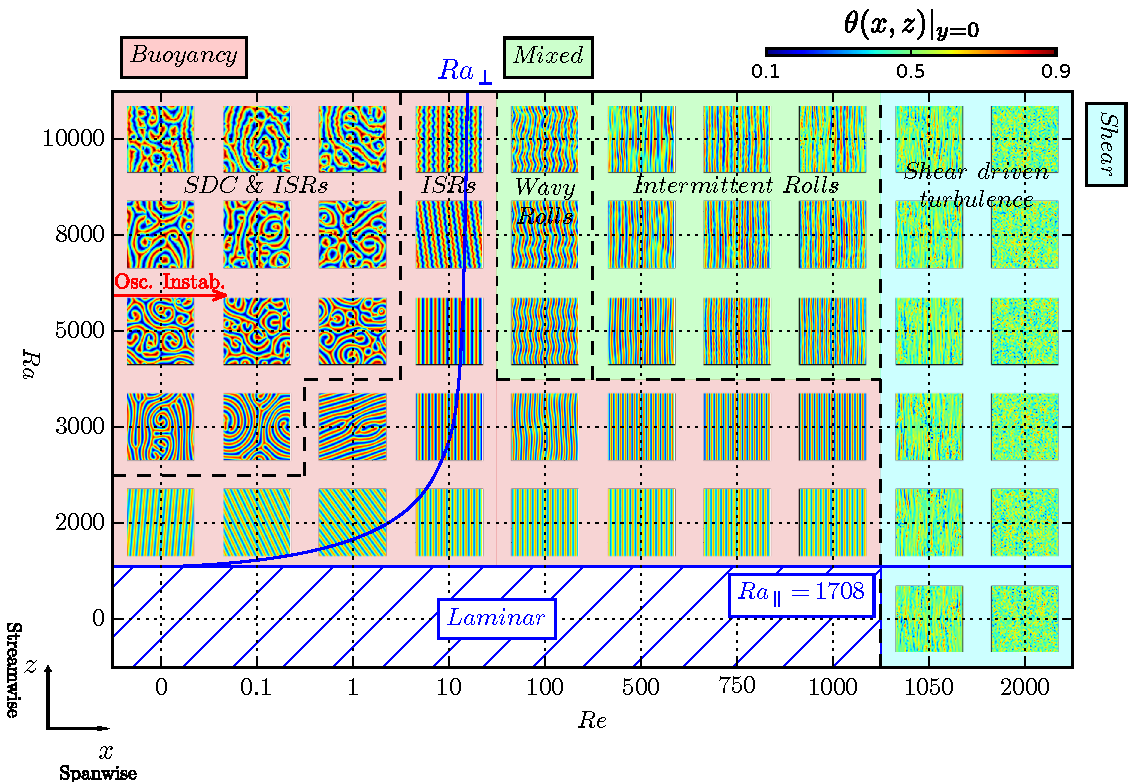
\includegraphics[width=1.3\textwidth, angle=90]{TransitionalRBP/Figures/PhaseSpace/RaRePhaseSpace.pdf}
    \caption{A \DIFdelbeginFL \DIFdelFL{conceptual diagram of he }\DIFdelendFL $Ra-Re$ phase space illustrates the midplane temperature snapshots, $\theta(x,z)|_{y=0}$ for $Re \in [0,2000]$ and $Ra \in [0, 10000]$, \DIFaddbeginFL \DIFaddFL{$\Gamma = 4\pi$, }\DIFaddendFL classified into five distinct regimes: (1) SDC \& ISRs, (2) ISRs, (3) wavy rolls, (4) intermittent rolls and (5) shear-driven turbulence. The blue solid curves refer to primary neutral curves of the longitudinal and transverse rolls $Ra_\parallel, Ra_\perp$. The red \DIFdelbeginFL \DIFdelFL{curve }\DIFdelendFL \DIFaddbeginFL \DIFaddFL{arrow }\DIFaddendFL indicates the secondary oscillatory instability of ISRs at $Re = 0$\DIFaddbeginFL \DIFaddFL{, $Ra \sim 6000$ }\DIFaddendFL \citep{bodenschatz_recent_2000}. Shades of red, green and blue indicate their dominant mechanism, whether driven by buoyancy or shear (or mixed). For $Re > 0$, the mean flow is along the $z$ direction.}
    \label{fig:rarephase}
\end{figure}

We present the results obtained from the DNS of transitional RBP flows, focusing on the parameter space defined by Rayleigh numbers in the range $Ra \in [0, 10000]$, and Reynolds numbers in the range of $Re \in [0, 2000]$ (see Appendix \ref{app:params} for the full details).

For all numerical simulations, \DIFdelbegin \DIFdel{an initial condition , }\DIFdelend \DIFaddbegin \DIFadd{the initial condition }\DIFaddend consists of a Gaussian white noise with zero mean and unit variance, superimposed onto the laminar base state (i.e. conduction state at $Re = 0$).
The RBP system is then time-integrated untila statistically stationary state is reached, which typically requires a time of $t = O(10)$ to $O(10^2)$.
At the two \DIFdelbegin \DIFdel{end points }\DIFdelend \DIFaddbegin \DIFadd{endpoints }\DIFaddend of the $Re$-spectrum considered (i.e. $Re = 0, 2000$), SDC and subcritical shear-driven turbulence appear.
Figure \ref{fig:rarephase} shows \DIFdelbegin \DIFdel{the }\DIFdelend snapshots of the midplane temperature, $\theta(x,z)|_{y=0}$, of different flow regimes \DIFdelbegin \DIFdel{on }\DIFdelend \DIFaddbegin \DIFadd{in }\DIFaddend the $Ra$-$Re$ phase space.
The solid blue curves \DIFdelbegin \DIFdel{represents to }\DIFdelend \DIFaddbegin \DIFadd{represent }\DIFaddend the neutral stability boundaries for the longitudinal and transverse rolls as $Ra_\parallel = 1708$ and $Ra_\perp = f(Re)$, respectively \citep{gage_stability_1968}.
In the absence of shear at $Re=0$, these curves merge into the classical critical RBC instability at $Ra_{c} = 1708$, as ISRs become rotationally invariant about the wall-normal axis.
ISRs may undergo secondary instability for $Ra > Ra_{\parallel}$, and an approximate boundary of this is indicated by a red arrow\DIFdelbegin \DIFdel{roughly indicates }\DIFdelend \DIFaddbegin \DIFadd{, roughly indicating }\DIFaddend the secondary neutral stability boundary, marking the onset of oscillatory instabilities of ISRs within $Ra \gtrsim 5000$ \citep{clever_transition_1974}.
We note that the phase diagram in figure \ref{fig:rarephase} is not-to-scale plotted\DIFaddbegin \DIFadd{, }\DIFaddend serving as a conceptual reference to \DIFdelbegin \DIFdel{distinugish }\DIFdelend \DIFaddbegin \DIFadd{distinguish }\DIFaddend between different flow states and their coarse-grained transition boundaries.

In this $Ra$-$Re$ phase space, we categorise the flow behaviour into five distinct regimes: (1) bistability between SDC and ISRs (SDC \& ISRs), (2) ideal straight rolls (ISRs), (3) wavy rolls, (4) intermittent rolls, and (5) shear-driven turbulence.
The categories are defined based on common flow structures (patterns), and/or dynamical characteristics, ranging from equilibrium solutions to intermittent and chaotic dynamics.
Furthermore, we sort out these states based on their first and second-order statistical properties, where they appear independent of $Re$ in the buoyancy-dominated regime (shaded in red), and $Ra$ in the shear-dominated regime (shaded in blue), discussed in detail in  \DIFdelbegin \DIFdel{Appendix \ref{app:statistics}}\DIFdelend \DIFaddbegin \DIFadd{Appendices \ref{app:buoyancy} and \ref{app:shear} respectively}\DIFaddend .
In the mixed regime shaded in green, both $Ra$ and $Re$ are important.

\begin{figure}[h]
    \centering
    \includegraphics[width=0.8\linewidth]{TransitionalRBP/Figures/PhaseSpace/Ra3kplots.pdf}
    \caption{Midplane temperature snapshots at $Ra = 3000$, (a) $Re = 0.1$, (b) $Re = 1$, (c) $Re = 10$, (d) $Re = 100$, (e) \DIFdelbeginFL \DIFdelFL{$Re = 500$}\DIFdelendFL \DIFaddbeginFL \DIFaddFL{$Re = 1000$}\DIFaddendFL , (f) \DIFdelbeginFL \DIFdelFL{$Re = 1000$}\DIFdelendFL \DIFaddbeginFL \DIFaddFL{$Re = 2000$}\DIFaddendFL .}
    \label{fig:Ra3k}
\end{figure}
Given that the buoyancy-dominated regime is relatively well studied (RBC flow, in particular), \DIFdelbegin \DIFdel{here we }\DIFdelend \DIFaddbegin \DIFadd{we will }\DIFaddend only provide a brief description of the simulation results in this regime, with further magnified flow fields shown in figure \ref{fig:Ra3k}.
In the buoyancy-dominated regime, the flow structures are predominantly organised with convection rolls, such as SDC, transverse, oblique, longitudinal rolls (and ISRs with no mean flow), or oscillatory rolls.
The bistability between SDC and ISRs \DIFdelbegin \DIFdel{is preserved for $Ra \geq 3000$ at $Re = 0.1$ }\DIFdelend (refer to figure \ref{fig:Ra3k}(a)) \DIFaddbegin \DIFadd{is preserved for $Ra \geq 3000$ at $Re = 0.1$  }\DIFaddend and $Re = 1$ for $Ra \geq 5000$ (see also figure \ref{fig:buoyancy_wavy_regime}(a,d,g)). There exists a maximum $Re$, beyond which SDC disappears, we denote this as $Re_s$, and its dependence on $Ra$ is demarcated by the black dashed lines on the left side of figure \ref{fig:rarephase}.
Notably, an oblique roll with a \DIFdelbegin \DIFdel{`hooked-like' }\DIFdelend \DIFaddbegin \DIFadd{hook-like }\DIFaddend defect is observed at $Re = 1$, $Ra = 3000$\DIFaddbegin \DIFadd{, }\DIFaddend shown in figure \ref{fig:Ra3k}(b), reminiscent of the multiple \DIFdelbegin \DIFdel{`}\DIFdelend non-ISR \DIFdelbegin \DIFdel{' }\DIFdelend states in RBC (see references in \S\ref{sec:bkgrd_RBC}).
At $Re = 10$, the SDC disappears and longitudinal rolls with a spanwise wavenumber of $\alpha d = 2.5$ emerge, illustrated in figure \ref{fig:Ra3k}(c), suggesting that the roll wavenumber \DIFdelbegin \DIFdel{adheres to }\DIFdelend \DIFaddbegin \DIFadd{is within }\DIFaddend the stability boundaries of the Busse balloon \DIFdelbegin \DIFdel{\mbox{%DIFAUXCMD
\cite[see also figure~6 in][]{bodenschatz_recent_2000}}\hspace{0pt}%DIFAUXCMD
}\DIFdelend \DIFaddbegin \DIFadd{(see also figure 6 in \mbox{%DIFAUXCMD
\citet{bodenschatz_recent_2000}}\hspace{0pt}%DIFAUXCMD
)}\DIFaddend .
As $Re$ is increased further to $1000$, the longitudinal rolls emerge as the preferred solution at $Ra = 2000, 3000$.
The non-dimensionalised spanwise wavenumber of \DIFaddbegin \DIFadd{the }\DIFaddend longitudinal rolls observed at $Ra = 3000$ and \DIFdelbegin \DIFdel{$Re = 100, 500, 10000$}\DIFdelend \DIFaddbegin \DIFadd{$Re = 100, 500$ (not shown) and  $Re=1000$}\DIFaddend , shown in figure \ref{fig:Ra3k}(\DIFdelbegin \DIFdel{d-f}\DIFdelend \DIFaddbegin \DIFadd{d-e}\DIFaddend ) respectively, is approximately $\alpha d \approx 3.3$, which lies outside of the stability boundaries of the Busse balloon in RBC \DIFdelbegin \DIFdel{\mbox{%DIFAUXCMD
\cite[figure 6 in][]{bodenschatz_recent_2000}}\hspace{0pt}%DIFAUXCMD
}\DIFdelend \DIFaddbegin \DIFadd{(see figure 6 in \mbox{%DIFAUXCMD
\citet{bodenschatz_recent_2000}}\hspace{0pt}%DIFAUXCMD
)}\DIFaddend .
This suggests that the stability boundaries of the longitudinal rolls may \DIFdelbegin \DIFdel{change as }\DIFdelend \DIFaddbegin \DIFadd{vary with increasing }\DIFaddend $Re$\DIFdelbegin \DIFdel{increases}\DIFdelend .
Interestingly, a stable \DIFdelbegin \DIFdel{`pinched ' }\DIFdelend \DIFaddbegin \DIFadd{pinched }\DIFaddend longitudinal roll pattern emerges at $Re = 100$ $Ra = 3000$, reminiscent of a \DIFdelbegin \DIFdel{skew-varicosed }\DIFdelend \DIFaddbegin \DIFadd{skew-varicose }\DIFaddend instability shown in figure \ref{fig:Ra3k}(d).
Unlike the secondary \DIFdelbegin \DIFdel{skewed-varicose }\DIFdelend \DIFaddbegin \DIFadd{skew-varicose }\DIFaddend instability observed in RBC (which reduces the wavenumber of an unstable ISR by pinching adjacent rolls together\DIFdelbegin \DIFdel{\mbox{%DIFAUXCMD
\cite[see figure 7]{bodenschatz_recent_2000}}\hspace{0pt}%DIFAUXCMD
}\DIFdelend \DIFaddbegin \DIFadd{, see figure 7 of \mbox{%DIFAUXCMD
\citet{bodenschatz_recent_2000}}\hspace{0pt}%DIFAUXCMD
}\DIFaddend ), a stable \DIFdelbegin \DIFdel{`pinched ' }\DIFdelend \DIFaddbegin \DIFadd{pinched }\DIFaddend tertiary state emerges here.
\DIFaddbegin \DIFadd{As $Re$ increases to $2000$, shear-driven turbulence emerges, depicted as a featureless temperature field driven by the underlying turbulent fluctuations in figure \ref{fig:Ra3k}(f).
}\DIFaddend 

Figure \ref{fig:buoyancy_wavy_regime} presents a detailed analysis of the coarse-grained transition boundaries between SDC and ISRs in the range $Re \in [1, 10]$, and from ISRs to wavy rolls for $Re \in [10, 100]$ across high Rayleigh numbers considered, $Ra \in [5000, 10000]$.
As $Re$ increases from $1$ to $10$, \DIFaddbegin \DIFadd{the }\DIFaddend SDC regime (see figure \ref{fig:buoyancy_wavy_regime}(a,d,g)) vanishes and longitudinal rolls emerge, as shown in figure \ref{fig:buoyancy_wavy_regime}(b,e,h) for $Ra = 10000, 8000, 5000$, respectively.
These longitudinal rolls may undergo short-wavelength modulations, \DIFdelbegin \DIFdel{indicative of }\DIFdelend \DIFaddbegin \DIFadd{corresponding to }\DIFaddend the secondary oscillatory instability of RBC occurring above $Ra \gtrsim 5000$ \citep{clever_transition_1974}.
This results in the development of oscillatory longitudinal rolls described by a relative periodic orbit at $Ra= 8000$, and a chaotic state at $Ra = 10000$, shown in figure \ref{fig:buoyancy_wavy_regime}(e,b) respectively.

The footprint of oscillatory convection rolls is also evident in the SDC regime at $Ra = 10000$, $Re = 1$, shown in figure \ref{fig:buoyancy_wavy_regime}(a).
As $Re$ increases from $10$ to $100$, the longitudinal rolls exhibit longer wavelength modulations, indicative of the wavy instability \citep{clever_instabilities_1991, pabiou_wavy_2005}.
This gives rise to wavy longitudinal rolls, appearing as a travelling wave, quasi-periodic tori, and a chaotic state at $Ra = 5000, 8000, 10000$, shown in figure \ref{fig:buoyancy_wavy_regime}(i,f,c) respectively.
The wavelengths of the streamwise waviness and the spanwise periodic longitudinal roll appear to be approximately \DIFdelbegin \DIFdel{three intervals of }\DIFdelend \DIFaddbegin \DIFadd{$1/3$ of the }\DIFaddend streamwise length, \DIFdelbegin \DIFdel{$\Lambda_z \sim L_z/3$, and twelve intervals of }\DIFdelend \DIFaddbegin \DIFadd{and $1/12$ of the }\DIFaddend spanwise length, \DIFdelbegin \DIFdel{$\Lambda_x \sim L_x/12$, }\DIFdelend respectively.
Hence, the ratio between the streamwise waviness wavelength and the spanwise roll is about $4$, consistent with the ratio observed by \DIFdelbegin \DIFdel{\mbox{%DIFAUXCMD
\cite{clever_instabilities_1991}}\hspace{0pt}%DIFAUXCMD
}\DIFdelend \DIFaddbegin \DIFadd{\mbox{%DIFAUXCMD
\citet{clever_instabilities_1991}}\hspace{0pt}%DIFAUXCMD
}\DIFaddend .


\begin{figure}
    \centering
    \includegraphics[width=1.2\linewidth, angle=90]{TransitionalRBP/Figures/PhaseSpace/BuoyancyRegime-minimal.pdf}
    \caption{The space-time plots of midplane temperature field, temperature snapshot and phase space trajectories of the Nusselt number against wall shear rate at  (a,b,c) $Ra = 10000$ for $Re = 1, 10, 100$; (d,e,f) $Ra = 8000$ for $Re = 1,10,100$; and (g,h,i) $Ra = 5000$ for $Re = 1, 10, 100$. The flow patterns are primarily organised into spiral defect chaos, longitudinal rolls, and wavy rolls \DIFdelbeginFL \DIFdelFL{occuring }\DIFdelendFL \DIFaddbeginFL \DIFaddFL{occurring }\DIFaddendFL at $Re = 1, 10, 100$, respectively.}
    \label{fig:buoyancy_wavy_regime}
\end{figure}

\subsection{Spatiotemporal intermittent rolls}\label{sec:intermittentrolls}
\begin{figure}
    \centering
    \includegraphics[width=\linewidth]{TransitionalRBP/Figures/PhaseSpace/Ra8000-Re500-BotSpaceTime-TimeHist.pdf}
    \caption{The intermittent rolls regime at $Ra = 8000, Re = 500$, $t \in [0, 10000]$. (a) The time history of shear on the lower wall and \DIFaddbeginFL \DIFaddFL{the }\DIFaddendFL Nusselt number. Space-time ($x$-$t$) plots of (b) near-wall wall-normal and spanwise perturbation kinetic energy and (c) midplane temperature space-time plot, with the corresponding near-wall and midplane temporal planar snapshots at (d,e) $t = 3736$, (f,g) $t = 6189$, and (h,i) $t = 8680$.}
    \label{fig:Ra8k-Re500-IntRolls}
\end{figure}

As $Re$ approaches $Re = 500$, the wavy rolls disappear.
Instead, a new regime, referred to as intermittent rolls, is observed.
In this regime, the longitudinal rolls remain as the dominant convection structure, interspersed with a spatio-temporal intermittent breakdown towards the laminar state.
This behaviour is illustrated for \DIFdelbegin \DIFdel{$(Ra,Re) = (8000,500$}\DIFdelend \DIFaddbegin \DIFadd{$(Ra, Re) = (8000,500$}\DIFaddend ) in figure \ref{fig:Ra8k-Re500-IntRolls}(a) using the temporal oscillations of the plane-averaged shear rate on the lower wall, $\langle \tau_w \rangle_{x,z}$, and the Nusselt number, $Nu$. 
We note \DIFaddbegin \DIFadd{that }\DIFaddend $\tau_w = 2$ and $Nu = 1$ for the laminar solution.

The spatio-temporal intermittent breakdown of the longitudinal rolls towards the laminar state is observed in figure \ref{fig:Ra8k-Re500-IntRolls}(b), where the bright and dark regions in the space-time plot of near-wall spanwise and wall-normal perturbation kinetic energy ($\mathcal{E}_{u'+v'} = 1/2(u'^2+ v'^2)$) at $(y^+,z)=(15,8\pi)$, highlight the co-existence of longitudinal rolls and spatially localised laminar states; here, $\mathbf{u}' = \mathbf{u} - W_{lam}(y)$ and \DIFdelbegin \DIFdel{$y^+ = (y+1)/Re_\tau$ with $Re_\tau=u_\tau h/\nu$}\DIFdelend \DIFaddbegin \DIFadd{$y^+ \equiv (y+1)/Re_\tau$ with $Re_\tau \equiv u_\tau h/\nu$}\DIFaddend , where $u_\tau$ is the friction velocity.
A similar observation is made with the space-time plot of midplane temperature, $\theta|_{(y,z)=(0,8\pi)}$, in figure \ref{fig:Ra8k-Re500-IntRolls}(c), where the elongated red/blue contours correspond to up-/down-welling regions of longitudinal rolls, and the green regions indicate spatially-localised laminar states.
The two near-wall transport properties, the wall shear rate and the Nusselt number, exhibit strong correlations.
For example, at $t = 3736$, both peaks reveal a spatially coherent longitudinal roll structure in figure \ref{fig:Ra8k-Re500-IntRolls}(d,e). There are also dips observed at $t = 6189$ and $t=8680$, indicative of the spatially local breakdown towards the laminar state, as shown in figures \ref{fig:Ra8k-Re500-IntRolls}(f,g) and \ref{fig:Ra8k-Re500-IntRolls}(h,i), respectively.
In summary, the longitudinal rolls enhance heat and momentum transfer towards the walls, but they appear to be intermittently disrupted by the breakdown towards the laminar state.
To better understand this behaviour, we later consider the temporal dynamics in a confined domain, $\Gamma = \pi / 2$, where the spatial intermittency is artificially suppressed (see \S \ref{sec:TASP}).

\subsection{Co-existence of convection rolls with turbulent bands}\label{sec:rbp_3.3}
\begin{figure}
\centering
\includegraphics[width=\linewidth]{TransitionalRBP/Figures/RaEffectOnTurbulence/Ra0-Re1050-3-BotSpaceTime-Lows.pdf}
\caption{Shear-driven turbulence regime at $Ra = 0, Re = 1050$, $t \in [0, 8000]$. Space-time plots of (a) near-wall wall-normal and spanwise perturbation kinetic energy, (b) midplane temperature space-time plot, and near-wall and midplane temporal planar snapshots at (c,d) $t = 1100$, (e,f) $t = 4491$, and (g,h) $t = 6171$, highlighting a prolonged laminar patch.}
\label{fig:spacetime-Ra0k-Re1.05k}
\end{figure}

As $Re$ approaches $Re = 1050$, shear-driven turbulence emerges as spatio-temporal intermittent turbulent-laminar bands, where turbulent and laminar regions can co-exist \citep{tuckerman_patterns_2020}.
In the absence of buoyancy (i.e. $Ra = 0$), these bands emerge clearly shown in figure \ref{fig:spacetime-Ra0k-Re1.05k}.
The space-time plot of the near-wall wall-normal and spanwise perturbation kinetic energy, $\mathcal{E}_{u'+v'}$ \DIFaddbegin \DIFadd{(here we use wall units to illustrate the near-wall turbulent streaks)}\DIFaddend , at $y^+ = 15$ in figure \ref{fig:spacetime-Ra0k-Re1.05k}(a) highlights this co-existence, where the turbulent and laminar regions are indicated by dark and bright areas, respectively.
In particular, a period of prolonged laminar state is observed at $t = 1100, 4491, 6171$, represented by localised green regions in the space-time plot of midplane temperature, $\theta|_{(y,z)=(0,8\pi)}$, in figure \ref{fig:spacetime-Ra0k-Re1.05k}(b).
The prolonged laminar states are also evident in the near-wall and midplane temporal snapshots of figures \ref{fig:spacetime-Ra0k-Re1.05k}(c-h), shown as large pockets of dark and green regions that fill approximately half of the spatial domain.

\begin{figure}
\centering
\includegraphics[width=\linewidth]{TransitionalRBP/Figures/RaEffectOnTurbulence/Ra10000-Re1050-BotSpaceTime-Highs.pdf}
\caption{Shear-driven turbulence regime at $Ra = 10000, Re = 1050$, $t \in [0, 8000]$. Space-time plots of (a) near-wall wall-normal and spanwise perturbation kinetic energy, (b) midplane temperature spacetime plot, and their corresponding near-wall and midplane temporal $x-z$ planar snapshots at (c,d) $t = 1282$, (e,f) $t = 5077$, and (g,h) $t = 6358$, highlighting the coexistence of longitudinal rolls and turbulent bands.}
\label{fig:spacetime-Ra10k-Re1.05k}
\end{figure}

Next, we consider the influence of buoyancy on the turbulent-laminar bands and compare two distinctly different cases of buoyancy using $Ra = 0$ and $Ra = 10000$ at $Re = 1050$.
In the latter case, the typical features of the turbulent-laminar bands depicted as alternate dark and bright bands are also seen in the space-time plot of near-wall wall-normal and spanwise perturbation kinetic energy, $\mathcal{E}_{u'+v'}$, in figure \ref{fig:spacetime-Ra10k-Re1.05k}(a).
However, some important differences emerge compared to the former case (in $Ra = 0$).
In particular, the midplane temperature snapshots, $\theta|_{(y,z)=(0,8\pi)}$, at $t = 1282, 5077, 6358$ in figures \ref{fig:spacetime-Ra10k-Re1.05k}(d,f,h) reveal some localised regions of streamwise-aligned red and blue contour stripes, likely indicating the presence of longitudinal rolls.
These longitudinal roll regions are typically located next to neighbouring turbulent (bright) regions in the near-wall perturbation kinetic energy snapshots in figures \ref{fig:spacetime-Ra10k-Re1.05k}(c,e,g), suggesting that longitudinal rolls co-exist with turbulent patches at $Ra = 10000$.
However, we caution that although they are relatively weak, similar red and blue contour stripes are also observed at $Ra = 0$, where longitudinal rolls are not expected, as shown in figure \ref{fig:spacetime-Ra0k-Re1.05k}(f). In this case, these weak elongated red and blue contour stripes are likely to be from the near-wall streaks.

Nonetheless, turbulence occurs more spatially intermittently at $Ra = 0$, containing prolonged pockets of laminar regions, while turbulent regions at $Ra = 10000$ appear more visibly consistently (compare figures \ref{fig:spacetime-Ra0k-Re1.05k}a with \ref{fig:spacetime-Ra10k-Re1.05k}a).
In other words, the presence of longitudinal rolls may promote turbulence locally, and we will investigate this issue further in \S \ref{sec:rbp_4}.

\section{The role of longitudinal rolls}\label{sec:rbp_4}
\subsection{The thermally-assisted sustaining process (TASP) in a confined domain}\label{sec:TASP}
\begin{figure}
    \centering
    \includegraphics[width=\linewidth]{TransitionalRBP/Figures/RaEffectOnTurbulence/Ra10000-Re1050-MidBotTimeHist-4x4.png}
    \caption{Intermittent dynamics in a confined domain at $Ra = 10000$, $Re = 1050$, $t\in[0,3000]$, $\Gamma = \pi/2$. The time history of the (a) Nusselt number and shear. Temporal snapshots of volumetric temperature, planar near-wall streamwise and spanwise perturbations at (b) $t = 1291.5$, (c) $t = 1480.5$, (d) $t = 1564.5$, (e) $t = 1711.5$. Longitudinal rolls and transient turbulence are observed at (b,d) and (c,e), respectively.}
    \label{fig:Ra10k-Re1050-small}
\end{figure}

Given the complexities in the spatio-temporal dynamics observed in \S\ref{sec:rbp_3},
we consider simulations confined to a domain defined by $\Gamma = \pi/2$, where longitudinal rolls and localised turbulence could be viewed as spatially isolated.
We start from a numerical simulation at $Ra = 10000$ and $Re=1050$ in $\Gamma = \pi/2$, integrated in time for $t \in [0, 3000]$. 
The initial condition has been sampled from a statistically stationary turbulent field at $Re = 2000$ for $Ra=10000$, and the $Re$ is then slowly lowered to $Re = 1050$.
The time history for $t \in [0, 3000]$ of the two near-wall transport properties, the Nusselt number and the shear rate on the lower wall, is presented in figure \ref{fig:Ra10k-Re1050-small}, together with snapshots of the temperature, $\theta(\mathbf{x})$, and the near-wall streamwise and spanwise perturbation velocities, $w'|_{y^+= 15}, v'|_{y^+=15}$ at selected times.
In this confined domain, the dynamics of the system \DIFdelbegin \DIFdel{exhibits }\DIFdelend \DIFaddbegin \DIFadd{exhibit }\DIFaddend temporal intermittency, where the solution trajectory appears to wander between longitudinal rolls and highly disorganised chaotic flow fields, characterised by low- and high-near-wall transport properties, respectively.

Starting from a longitudinal roll state of spanwise wavenumber of $\alpha d = 4$ at $t = 1291.5$ in figure \ref{fig:Ra10k-Re1050-small}(b), the solution erupts into a highly disorganised turbulent state at $t = 1480.5$, marked by a disordered temperature field in figure \ref{fig:Ra10k-Re1050-small}(c).
During this breakdown, the near-wall snapshots of streamwise perturbation velocity, $w'|_{y^+ = 15}$, and wall-normal perturbation velocity, $v'|_{y^+ = 15}$, illustrated in the bottom panels of figures \ref{fig:Ra10k-Re1050-small}(c), reveal three pairs of high- and low-speed streaks, each with an average spanwise wavelength of $\Lambda_x^+ \approx 339/3 = 113$ (where $\Lambda_x^+ = u_\tau \Lambda_x / \nu$ \DIFdelbegin \DIFdel{refers to }\DIFdelend \DIFaddbegin \DIFadd{is the }\DIFaddend non-dimensionalised wavelength \DIFaddbegin \DIFadd{by wall units}\DIFaddend ), close to the mean streak spacing ($\Lambda^+_x \sim 100$) commonly reported in shear flow turbulence \citep{kline_structure_1967, kim_turbulence_1987, hamilton_regeneration_1995}.
These streaks appear to be meandering, negatively correlated with wall-normal perturbation velocities, reminiscent of a streak breakdown process \citep{hamilton_regeneration_1995}, or a bursting event \citep{kim_production_1971}, where high (low)-speed streaks are brought close to (away from) the wall, enhancing near-wall transport quantities.
The enhancement is reflected in large increments in the Nusselt number and wall shear rate of roughly $40\%$ at $t = 1480.5$ in figure \ref{fig:Ra10k-Re1050-small}(a).
Subsequently, the solution trajectory returns to a longitudinal roll state at $t=1564.5$, before erupting into turbulence at $t = 1711.5$ (see figures \ref{fig:Ra10k-Re1050-small}(d,e) respectively).
This suggests that the turbulence has a finite lifetime, occurring transiently before decaying towards the laminar state at $Re = 1050$ \citep{hof_finite_2006, schneider_turbulence_2007}, which is linearly unstable, leading to the onset of longitudinal rolls where transient turbulence could be re-excited again.

\begin{figure}
    \centering
    \includegraphics[width=\linewidth]{TransitionalRBP/Figures/RaEffectOnTurbulence/Ra0-Re1050-MidBotTimeHist.png}
    \caption{Relaminarisation in a confined domain at $Ra = 0$, $Re = 1050$, $t\in[0,3000]$, $\Gamma = \pi/2$. The time history of the (a) Nusselt number and shear. Temporal snapshots of volumetric temperature at (b) $t = 31.5$, (c) $t = 63$, (d) $t = 157.5$, (e) $t = 672$.}
    \label{fig:Ra0k-Re1050-small}
\end{figure}

To test this hypothesis, we consider a numerical simulation at $Ra = 0$, $Re = 1050$, in $\Gamma = \pi / 2$, where longitudinal rolls cannot appear.
The initial condition is taken from a stationary turbulent solution at a higher $Re$ of $Re = 2000$, which is then slowly lowered to $Re = 1050$, and then integrated in time for $t \in [0, 700]$.
The time history of the Nusselt number, $Nu$, and the wall shear rate, $\langle \tau_w \rangle_{x,z}$, is reported in figure \ref{fig:Ra0k-Re1050-small}, with the temperature snapshots, $\theta(\mathbf{x})$, at selected time units. 
An initial turbulent flow field decays towards the laminar solution in $t \in [0, 700]$.
Comparing the results between $Ra = 0$ and $Ra = 10000$, we propose that the longitudinal rolls at $Ra= 10000$ could mediate a transition mechanism between unstable laminar state and transient turbulence, so that the entire nontrivial flow dynamics could be sustained indefinitely.

\begin{figure}
    \centering
    \includegraphics[width=\linewidth]{TransitionalRBP/Figures/RaEffectOnTurbulence/T1620-MidBotTimeHist-Quenched-Annotated.pdf}
    \caption{$Ra$-quenching experiments for $Ra = 8000, 5000, 3000, 2000$, at $Re = 1050$, $\Gamma = \pi/2$, $t \in [850.5, 5000]$. The time history of (a) shear and (b) volumetric temperature snapshots of the flow condition at $t = 850.5$. Volumetric temperature snapshots for $Ra = 8000$ at (c,d) $t = 1312.5, 1743$, and $Ra = 5000$ at (e,f) $t = 1312.5, 3570$, revealing a longitudinal roll and a turbulent state, respectively. Stable longitudinal rolls emerge for $Ra = 3000$ at (g,h) $t = 1312.5, 4200$, and $Ra = 2000$ at (j,k) $t = 1312.5, 4200$.}
    \label{fig:RaQuench}
\end{figure}

Next, we investigate the impact of longitudinal rolls on this proposed mechanism at different $Ra$.
We \DIFdelbegin \DIFdel{capture the flow quantities }\DIFdelend \DIFaddbegin \DIFadd{save the flow }\DIFaddend for $Ra=10000$ and $Re=1050$ at $t=850.5$ (just before the onset of longitudinal rolls, see figure \ref{fig:Ra10k-Re1050-small}), and use \DIFaddbegin \DIFadd{the flow }\DIFaddend as an initial condition to perform four numerical simulations by lowering $Ra$ instantly to $Ra=8000,5000,3000,2000$, respectively\DIFdelbegin \DIFdel{and }\DIFdelend \DIFaddbegin \DIFadd{, and we then }\DIFaddend time-integrated further to $t \in [850.5, 5000]$.
The time history of the wall shear rate, $\langle \tau_w\rangle_{x,z}$, and the temperature snapshots, $\theta(\mathbf{x})$, of these experiments of \DIFdelbegin \DIFdel{`}\DIFdelend $Ra$-quenching \DIFdelbegin \DIFdel{' }\DIFdelend are presented in figure \ref{fig:RaQuench}.
The time history of shear is visibly intermittent for $Ra = 8000, 5000$, depicted as the orange and green trajectories in figure \ref{fig:RaQuench}(a), similar to $Ra = 10000$.
At $Ra= 8000, 5000$, the longitudinal rolls emerge approximately at $t = 1312.5$ (see figures \ref{fig:RaQuench}(c,e)), before erupting into turbulence at $t = 1743$ and $t = 3570$ in figures \ref{fig:RaQuench}(d,f), respectively.
This is then accompanied by a large spike in the wall shear rate before dipping briefly, shown as the orange and green trajectories of figure \ref{fig:RaQuench}(a).
As $Ra$ is lowered further to $Ra = 3000, 2000$, the transients begin to decay into a longitudinal state from $t = 850.5$ to $t = 1312.5$, which remains stable until $t = 4200$ illustrated by figure \ref{fig:RaQuench}(h,j), accompanied by the red and purple asymptotic trajectories in figure \ref{fig:RaQuench}(a). 
This suggests that the longitudinal rolls are likely to be linearly unstable for $Ra = 8000, 5000$, leading to turbulence, while remaining stable for $Ra = 3000,2000$.
In particular, the longitudinal roll state at $Ra = 5000$ remained saturated for a longer period $t \in [1500, 3400]$ (green curve in figure \ref{fig:RaQuench}(a)), indicating that the growth rate of the linear instability is smaller than for $Ra =  8000$.
We note that the longitudinal rolls in figure \ref{fig:RaQuench} have a spanwise wavenumber of $\alpha d=4$, which corresponds to the wavenumber of the dominant primary instability (see Appendix \ref{app:long-pri}), indicating that it is the most preferred wavenumber within the confined domain.

\begin{figure}
    \centering
    \includegraphics[width=\linewidth]{TransitionalRBP/Figures/RaEffectOnTurbulence/ev-compiled.pdf}
    \caption{The growth rates of infinitesimal perturbations linearised about longitudinal rolls, $\mathbf{q}_{LR}$, of spanwise wavenumber of $\alpha d = 4$, against (a) streamwise wavenumber $\beta d$, and (b) $Ra$ for $\beta d =2$. The hatches in (a) refer to wavenumbers smaller than those admissible in $\Gamma = \pi/2$. The dash-dotted line in (b) is a standard quadratic regression yielding $Ra_{s}\approx 4720$.}
    \label{fig:SecStabLongRolls}
\end{figure}

To understand the stability characteristics of the longitudinal rolls, we perform a linear stability analysis about the longitudinal roll state ($\alpha d= 4$), at $Ra = 10000, 8000, 5000, 3000, 2000$.
The details of linear stability analysis are described in \S\ref{sec:linearstab}, where $\lambda$ and $\mathbf{\breve{q}}(x,y)e^{i\beta z}$ refer to the eigenvalue and eigenmode.
The longitudinal roll (base) states, $\mathbf{q}_{LR}$, are obtained by time integrating an initial condition consisting of the laminar (conduction) state, superimposed by the primary eigenmode, $\alpha d = 4$, at $Ra = 10000, 8000, 5000, 3000, 2000$, in a two-dimensional $x-y$ plane, suppressing any three-dimensional perturbations numerically.
The growth rates as a function of discrete streamwise wavenumbers, $2 \leq \beta d \leq 5$, are presented in figure \ref{fig:SecStabLongRolls}.
We note that the admissible streamwise wavenumbers within $\Gamma = \pi/2$ are $\beta d = m$, where $m$ is a positive even integer, $m = 2, 4, ..$, and $\beta d = 3, 5$ are included for completeness.
The longitudinal rolls are linearly unstable for $Ra \geq 5000$, while they remain stable for $Ra \leq 3000$, which confirms our hypothesis earlier. 
In particular, the growth rates between $Ra = 5000$ and $Ra = 10000$ differ by an order of magnitude, which could explain the prolonged period of saturation in the green curve of figure \ref{fig:RaQuench}(a).
The dominant secondary instability of longitudinal rolls in $\Gamma = \pi / 2 $ has a streamwise wavenumber of $\beta d = 2$.
Using a standard quadratic regression, the critical Rayleigh number for disturbances with $\beta d = 2$ is approximately $Ra_{s} \approx 4720$, presented in figure \ref{fig:SecStabLongRolls}(b).

\begin{figure}
    \centering
    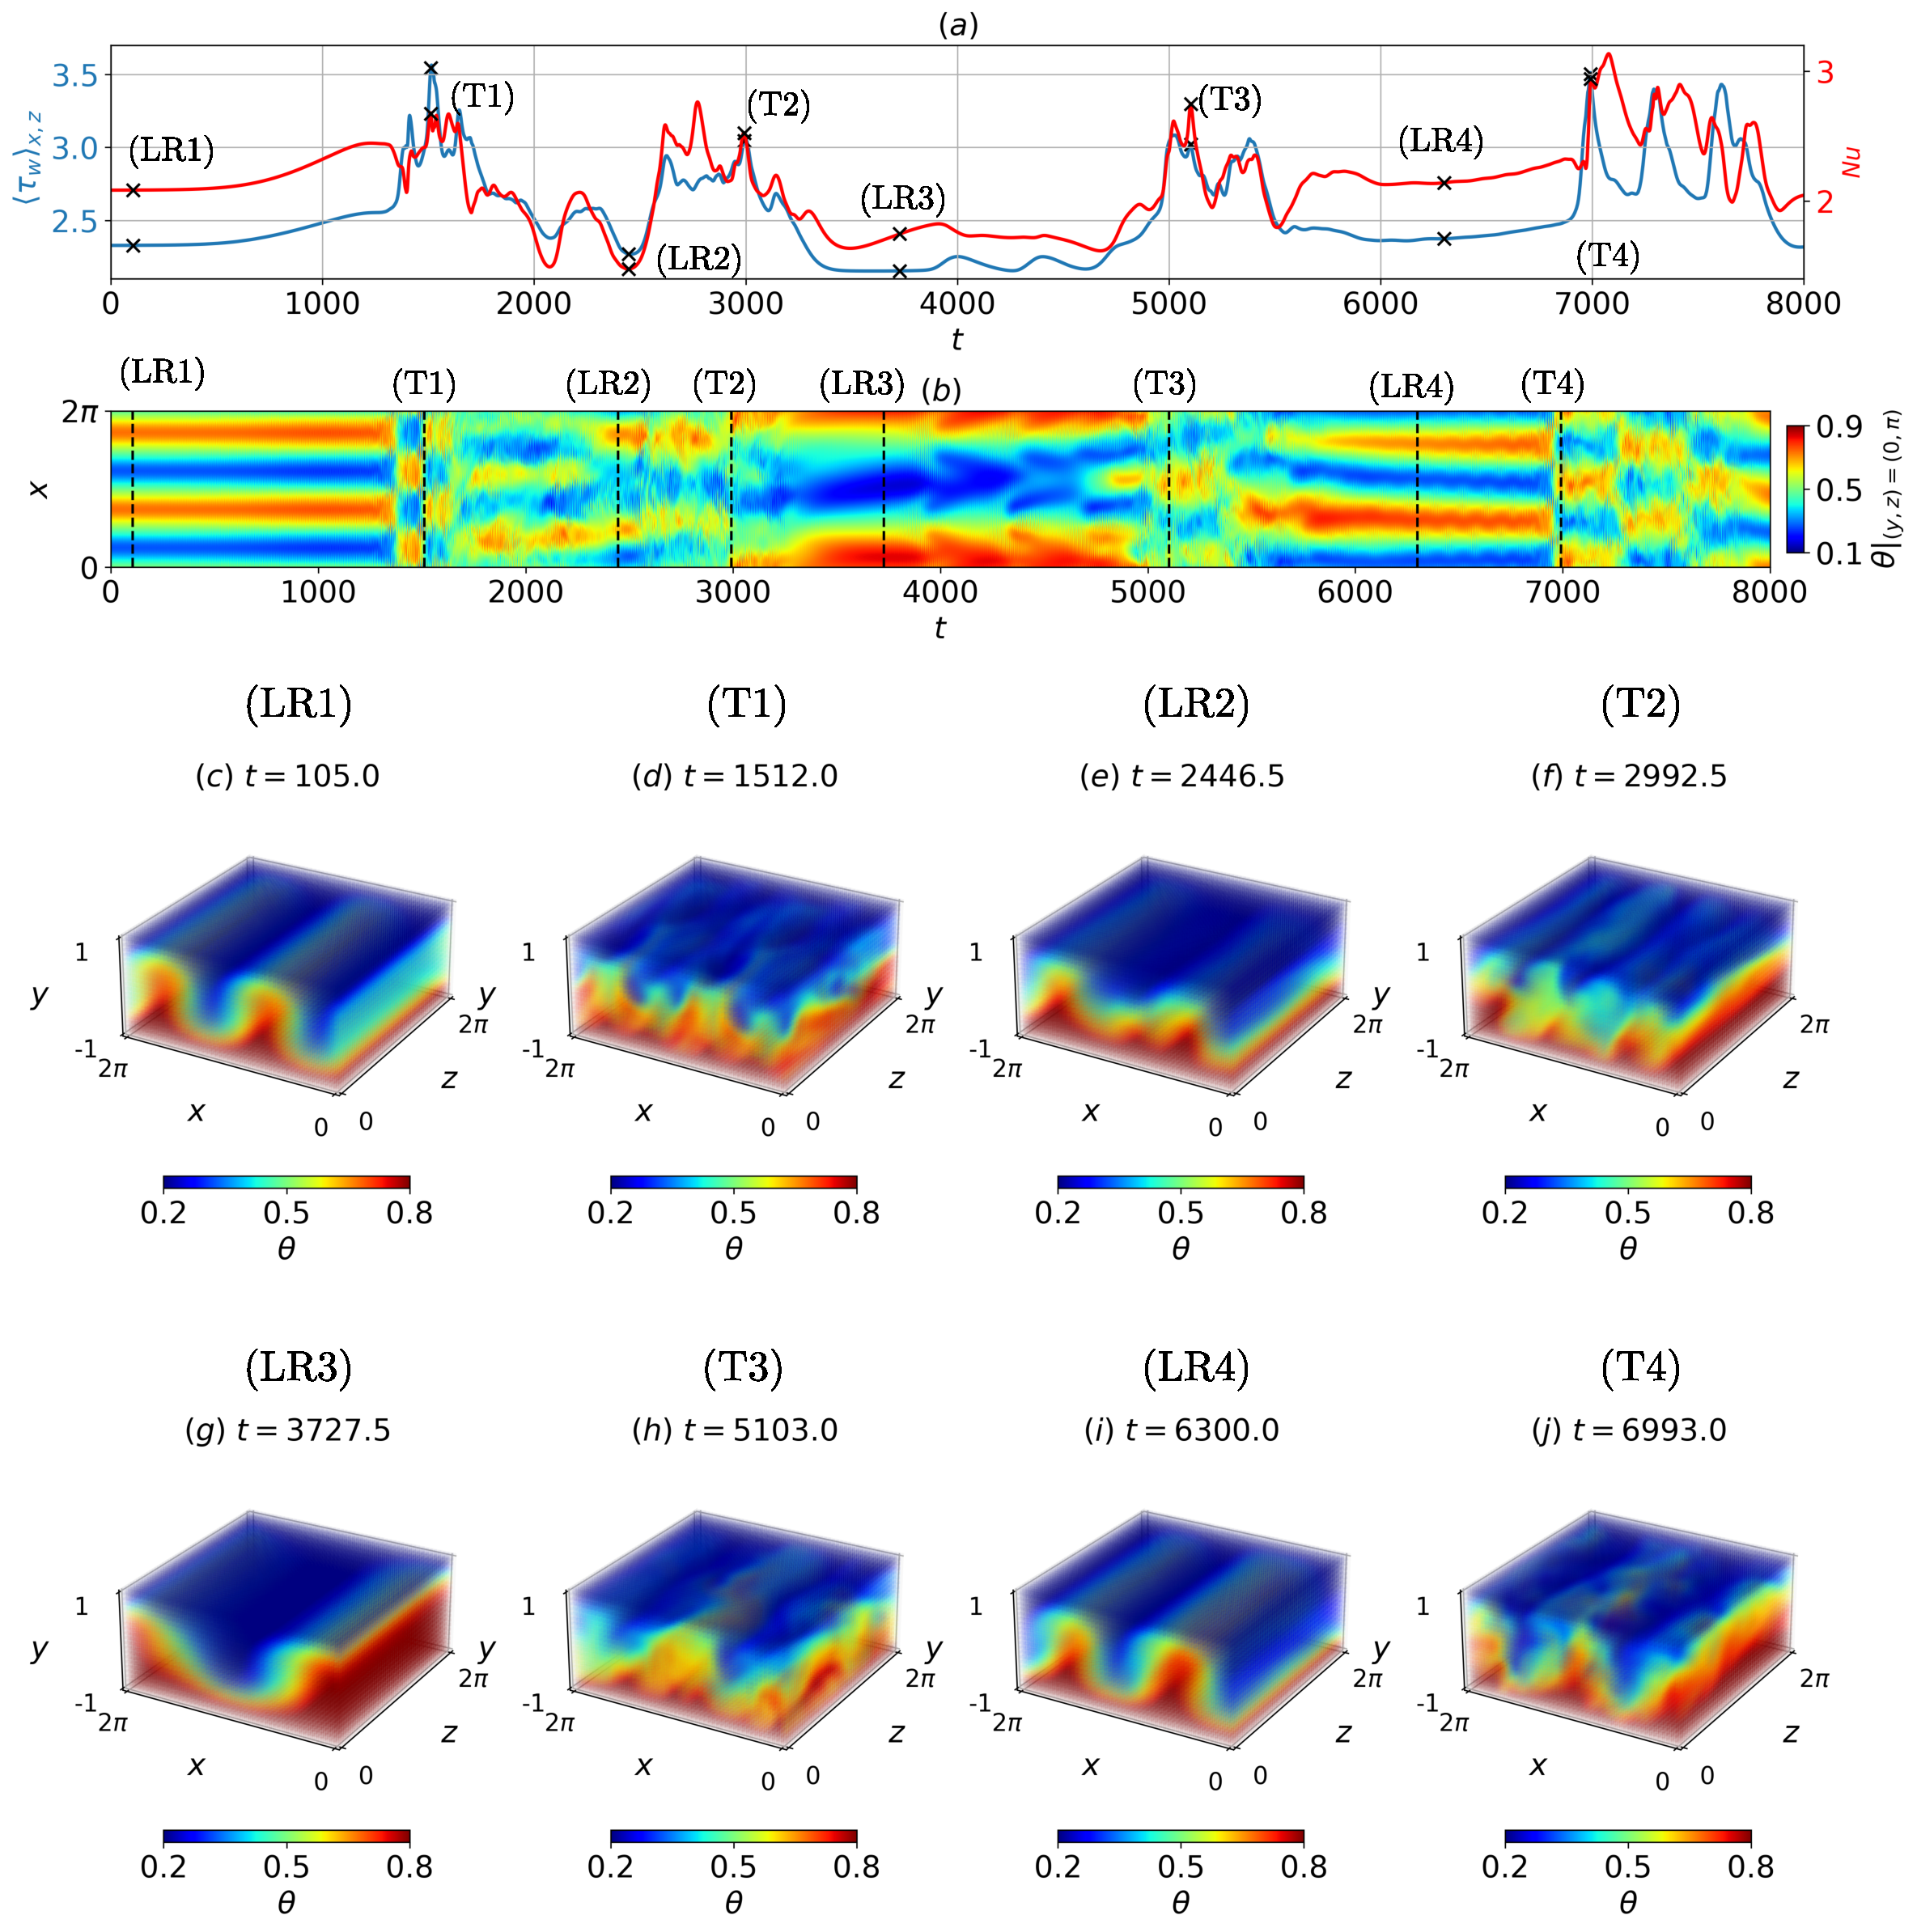
\includegraphics[width=\linewidth]{TransitionalRBP/Figures/RaEffectOnTurbulence/Ra5000-Re1050-MidBotTimeHist-PEig-minimal-labelled.pdf}
    \caption{Time integration along the dominant unstable \DIFdelbeginFL \DIFdelFL{manifold}\DIFdelendFL \DIFaddbeginFL \DIFaddFL{eigenmode}\DIFaddendFL , $\beta d =2$, of the longitudinal rolls at $Ra = 5000, Re = 1050, \Gamma = \pi/2$ for $t\in[0,8000]$. Time history of the (a) Nusselt number and wall shear rate, and (b) midplane temperature space-time plot. This system oscillates between the longitudinal rolls ($LR1-4$) and turbulence ($T1-4$) over four intervals. Snapshots of temperature at (c) $t = 105$, (d) $t = 1512$, (e) $t = 2446.5$, (f) $t = 2992.5$, (g) $t = 3727.5$, (h) $t = 5103$, (i) $t = 6300$, (j) $t = 6993$.}
    \label{fig:intermittent-dynamics}
\end{figure}

Following this, we examine the dominant unstable \DIFdelbegin \DIFdel{manifold }\DIFdelend \DIFaddbegin \DIFadd{eigenmode }\DIFaddend ($\beta d = 2$) of the longitudinal rolls ($\alpha d = 4$) at $Ra=5000$, by considering an initial condition
\DIFdelbegin \DIFdel{,
}\DIFdelend \begin{equation}\label{eq:SecInstab}
\mathbf{q}_0(\mathbf{x},t=0) = \mathbf{q}_{LR}(x,y) + (\mathbf{\breve{q}}(x,y)e^{i\beta z}+c.c).
\end{equation}
Here, $\breve{\mathbf{q}} e^{i\beta z}$ is an eigenmode for the streamwise wavenumber $\beta$, and its amplitude was scaled such that its total energy is
\DIFdelbegin \DIFdel{defined by
}\DIFdelend \begin{equation}\label{eq:totalenergy}
\delta \DIFdelbegin \DIFdel{= }\DIFdelend \DIFaddbegin \DIFadd{\equiv }\DIFaddend \frac{1}{{V}} \int_\Omega (\mathbf{\hat{u}}(\mathbf{x})^T\mathbf{\hat{u}}(\mathbf{x}) + \frac{Ra}{8Re^2Pr}\hat{\theta}(\mathbf{x})^2 )\; \mathrm{d}\Omega = 10^{-3}.
\end{equation}
We have also considered \DIFdelbegin \DIFdel{that }\DIFdelend $\delta = 10^{-2}, 10^{-4}$, but $\delta = 10^{-3}$  was found to be small enough to ensure linear growth while large enough without requiring a large number of time steps.

The initial condition is time-integrated for $t \in [0, 8000]$, and \DIFdelbegin \DIFdel{its }\DIFdelend \DIFaddbegin \DIFadd{the }\DIFaddend time history of the near-wall transport properties, the space-time plot of the mid-plane temperature, $\theta|_{(y,z)=(0,\pi)}$, are presented in figure \ref{fig:intermittent-dynamics}, with snapshots of temperature, $\theta(\mathbf{x})$, and near-wall streamwise and spanwise perturbation velocities, $w'|_{y^+= 15}, v'|_{y^+=15}$ at some selected times. 
The intermittent trajectory is visually apparent, oscillating between longitudinal rolls and transient turbulence over four cycles for $t \in [0, 8000]$: for example, the regions of low and high near-wall transport quantities in figure \ref{fig:intermittent-dynamics}(a) correspond well to the organised and disorganised longitudinal rolls in figure \ref{fig:intermittent-dynamics}(b), respectively.
As the solution emerges from the unstable \DIFdelbegin \DIFdel{manifold }\DIFdelend \DIFaddbegin \DIFadd{eigenmode }\DIFaddend of the longitudinal roll state, $(LR1)$ in figure \ref{fig:intermittent-dynamics}(c), the trajectory erupts into turbulence at $t = 1512$, marked by a disordered volumetric temperature field in snapshot $(T1)$ in figure \ref{fig:intermittent-dynamics}{\color{blue}(d)}.
Turbulence occurs transiently, and the solution decays towards a longitudinal roll-like state at $t = 2446.5$, shown by snapshot $(LR2)$ in figure \ref{fig:intermittent-dynamics}(e), forming a single cycle.
The intermittent cycle repeats over three subsequent intervals, where the transient turbulent state and longitudinal rolls emerge at $t = 2992.5, 5103, 6993$, and $t = 3727.5, 6300$, as shown in the snapshots $(T2,3,4)$ and $(LR3,4)$ in figures \ref{fig:intermittent-dynamics}(f,h,j) and \ref{fig:intermittent-dynamics}(g,i), respectively.
Lastly, we show that the dominant unstable \DIFdelbegin \DIFdel{manifold }\DIFdelend \DIFaddbegin \DIFadd{eigenmode }\DIFaddend of the longitudinal rolls is connected to a transient turbulent state.
Interestingly, a longitudinal roll with $\alpha d = 2$ sometimes emerges after turbulence decays, shown as the snapshot $(LR3)$.
This suggests that other unstable \DIFdelbegin \DIFdel{manifolds }\DIFdelend \DIFaddbegin \DIFadd{eigenmodes }\DIFaddend may well be linked to the transition to transient turbulence.

\begin{figure}
    \centering
    \includegraphics[width=\linewidth]{TransitionalRBP/Figures/RaEffectOnTurbulence/Ra5000-Re1050-StateSpace-dudy.png}
    \caption{State space projection based on the planar averaged centerline velocity and shear, coloured by the volume normalised perturbation kinetic energy at $Ra = 5000$, $Re = 1050$, $\Gamma = \pi/2$, (a) $t \in[0,800]$, (b) $t \in [0, 68750]$.  The open black circles represent the unstable equilibria of longitudinal rolls and the laminar state. Note that the black-crosses, labelled by (T1-4) and (LR1-4), refer to temporal snapshots in figure \ref{fig:intermittent-dynamics}, not equilibria solutions.}
    \label{fig:intermittent-state-space}
\end{figure}

To better visualise the temporal dynamics in figure \ref{fig:intermittent-dynamics}, we project the solution trajectory onto the space composed of two state observables: planar averaged centerline velocity, $\langle w|_{y=0} \rangle _{x,z}$, the wall shear rate, $\langle \tau_w\rangle_{x,z}$ coloured by the volume-averaged perturbation kinetic energy, $1/(2V)||\mathbf{u}'||^2$, in figure \ref{fig:intermittent-state-space}, where $\|\mathbf{u}'\|^2=\int_\Omega \mathbf{u}'^H\mathbf{u}' dV$ with $\Omega$ being the flow domain.
These observables are chosen because they are found to distinguish well the regions of turbulent states, longitudinal roll states, and the laminar state that reside around $(0.82, 3.2)$, $(0.90, 2.32)$, and at $(1, 2)$, respectively. Indeed, the temporal snapshots of $(T1-4)$ appear around the representative location of turbulent states, $(0.82, 3.2)$, and the snapshots of $(LR1-4)$ and an equilibrium related to the longitudinal roll state with the spanwise wavenumber $\alpha d=4$ (denoted by $\mathbf{q}_{LR, \alpha d = 4}$) are seen around $(0.90, 2.32)$.

The solution trajectory emerges from the unstable manifold of the longitudinal roll state, $\mathbf{q}_{LR_{\alpha d = 4}}$, evolving towards turbulent states around $(0.85,3.2)$, characterised by a high wall shear rate.
At this $Re$, the turbulence is transient in the confined domain, occurring with a finite lifetime, eventually decaying towards the laminar state \citep{zammert_streamwise_2014, tuckerman_patterns_2020, paranjape_direct_2023}.
As the solution trajectory approaches the laminar solution at $(1,2)$, it abruptly reverses towards the longitudinal roll state near $(0.95, 2.15)$, $(LR3)$ due to the buoyancy-driven linear instability of the laminar base state in the RBP flow. 
Subsequently, the solution trajectory \DIFdelbegin \DIFdel{could depart }\DIFdelend \DIFaddbegin \DIFadd{again departs }\DIFaddend along an unstable \DIFdelbegin \DIFdel{manifold }\DIFdelend \DIFaddbegin \DIFadd{eigenmode }\DIFaddend of the longitudinal rolls\DIFdelbegin \DIFdel{again}\DIFdelend , forming a cyclic process.

To see if this cycle could be sustained indefinitely, we consider a longer time horizon, $t \in [0, 68750]$, illustrated in figure \ref{fig:intermittent-state-space}(b).
The solution trajectory wanders between the `cloud' of transient turbulence at the top left corner (in red), and longitudinal roll and laminar states (in blue) in the bottom right, forming a \DIFdelbegin \DIFdel{basin of attraction }\DIFdelend \DIFaddbegin \DIFadd{cycle }\DIFaddend between the unstable longitudinal rolls, transient turbulence, and the unstable laminar base state.
This \DIFdelbegin \DIFdel{basin of attraction }\DIFdelend \DIFaddbegin \DIFadd{cycle }\DIFaddend is likely established above a critical $Ra$ as the longitudinal rolls become linearly unstable (i.e. $Ra \gtrsim Ra_{s} \approx 4720$, see figure \ref{fig:SecStabLongRolls}(b)), and the instability of the longitudinal rolls provides an intermediate pathway towards transient turbulence, which could be regenerated again - a \DIFdelbegin \DIFdel{`}\DIFdelend self-sustaining \DIFdelbegin \DIFdel{' }\DIFdelend dynamical process.
We refer to this process as the \emph{thermally-assisted sustaining process (TASP)}, inspired by the self-sustaining process (SSP) from turbulent shear flows (see \S \ref{subsec:SSP}).
A schematic of the \textit{TASP} is illustrated in figure \ref{fig:tasp}.

\begin{figure}
    \centering
    \includegraphics[width=0.7\linewidth]{TransitionalRBP/Figures/RaEffectOnTurbulence/TASP-graphics.pdf}
    \caption{The thermally-assisted sustaining process (TASP).}
    \label{fig:tasp}
\end{figure}

\subsection{Variation of $Ra$ and $Re$ on the thermally-assisted sustaining process in $\Gamma = \pi/ 2$}\label{sec:IntConfined}

\begin{figure}
\centering
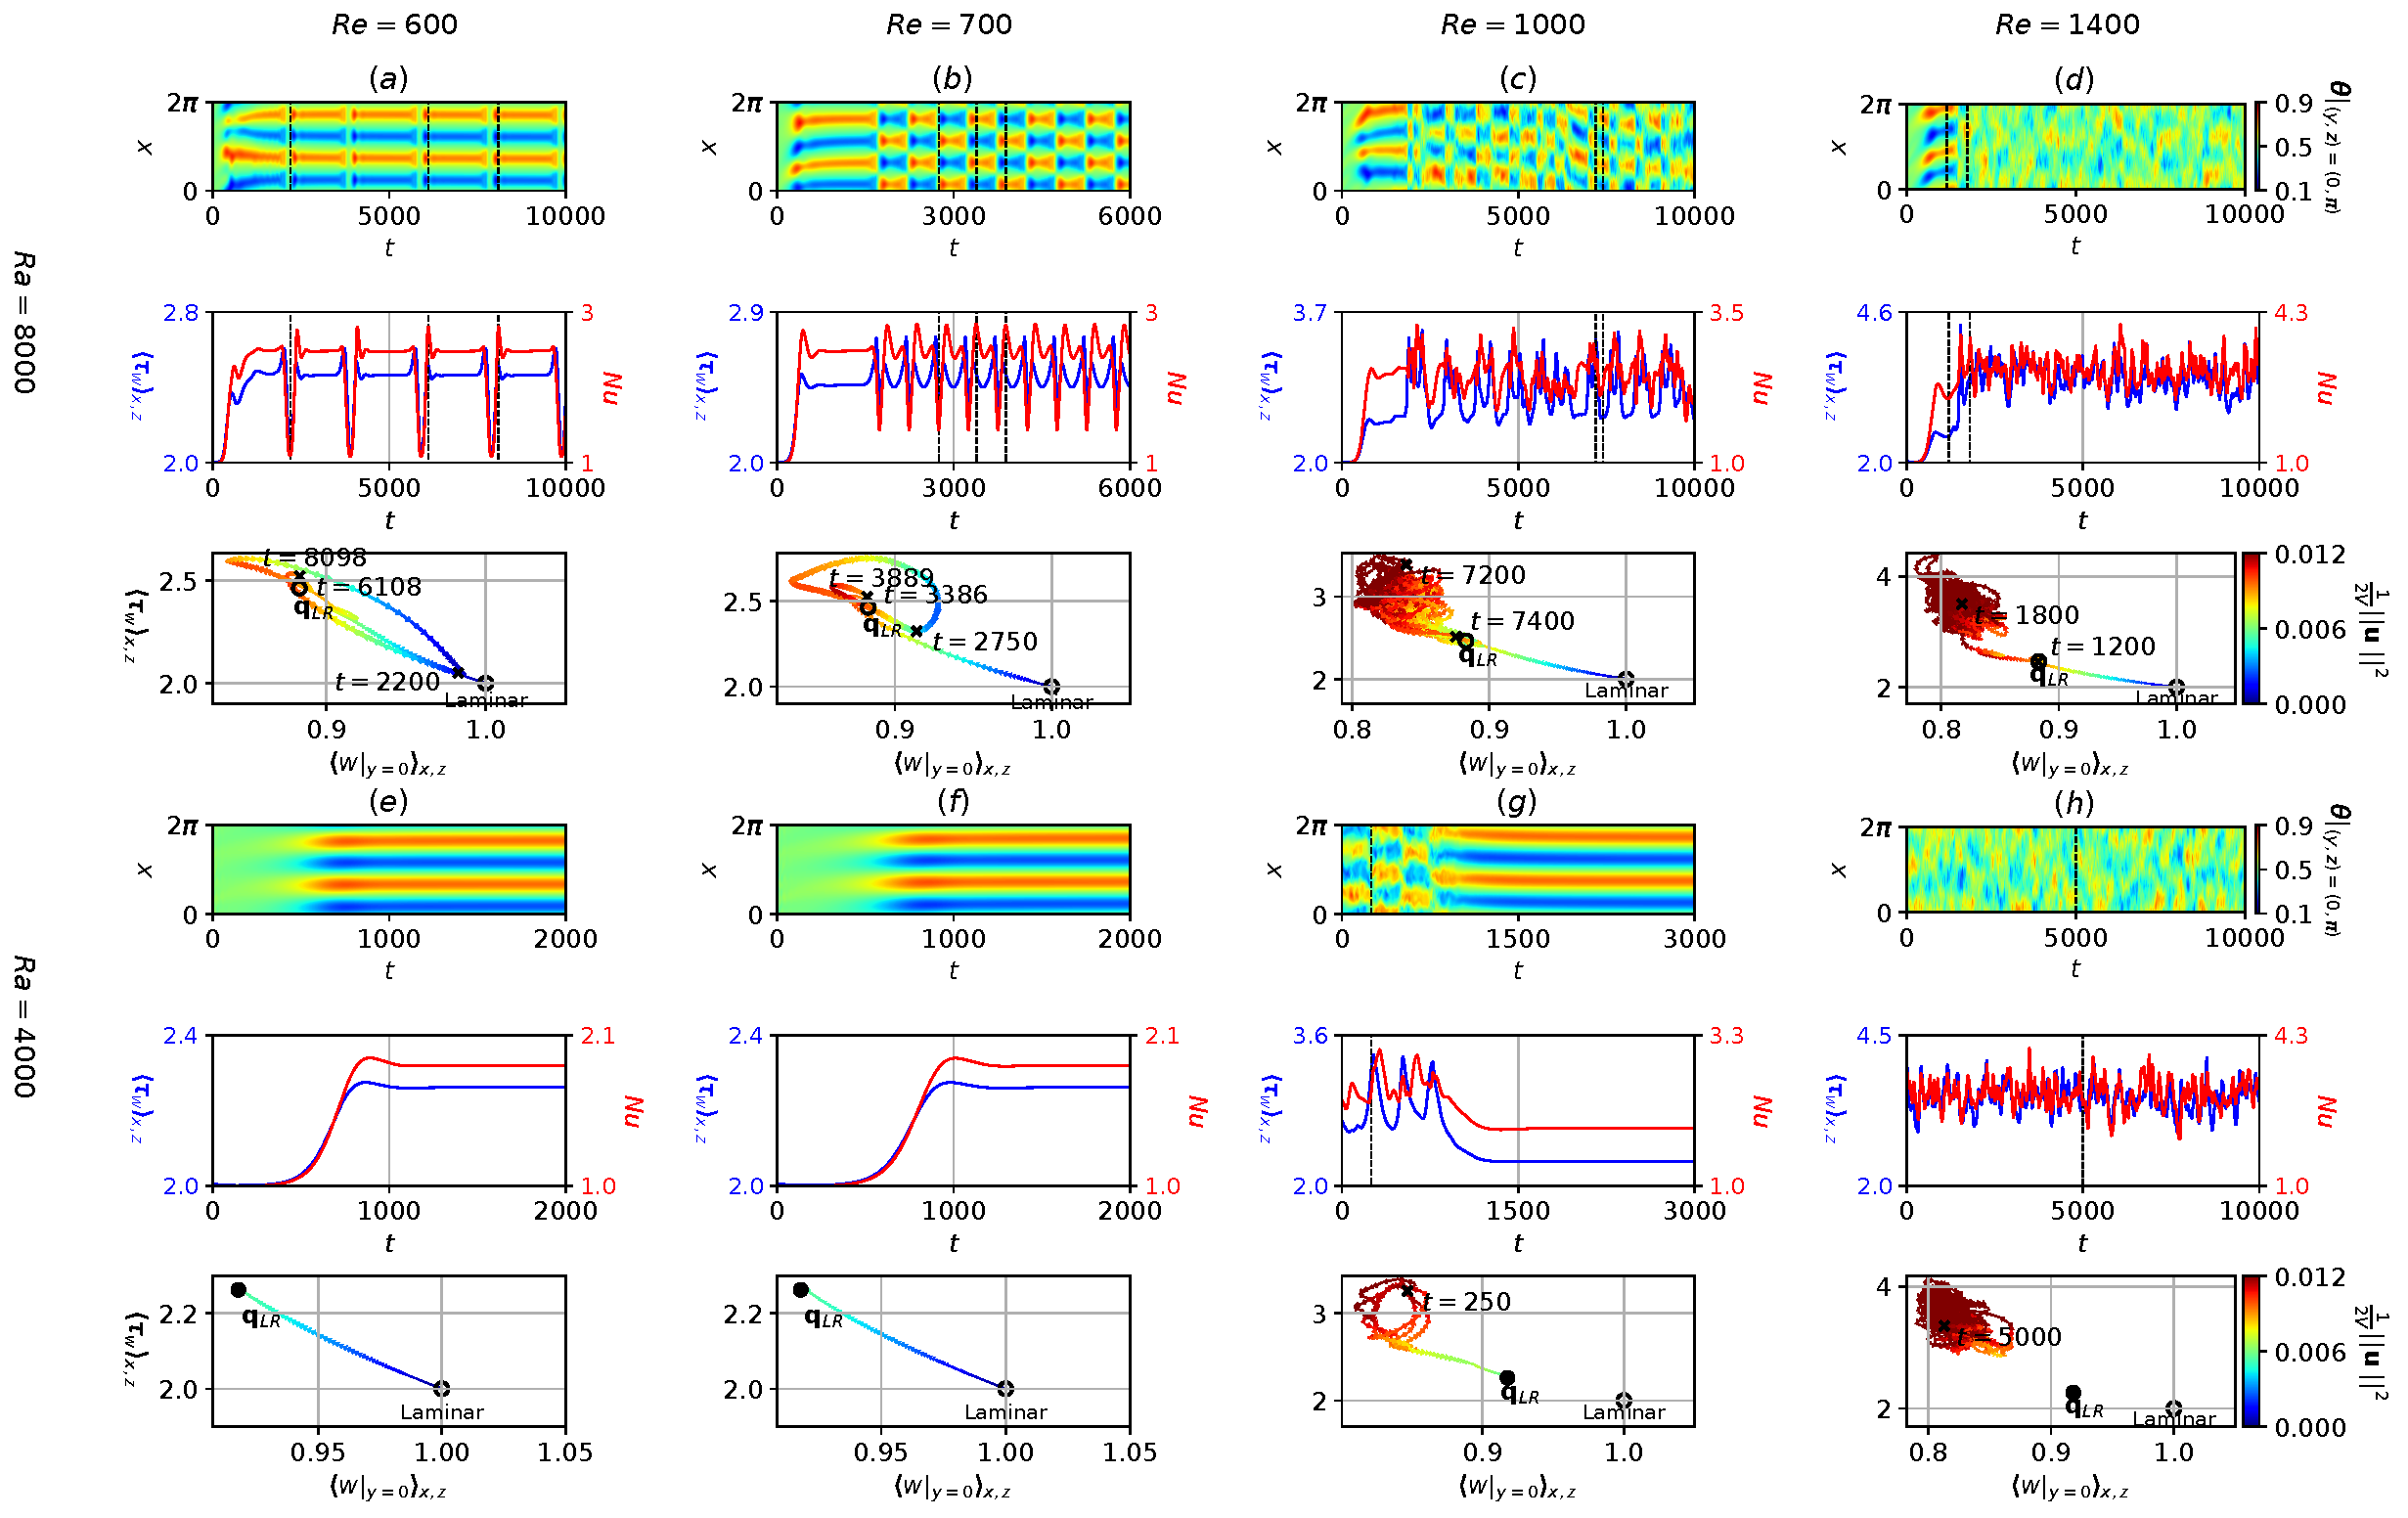
\includegraphics[width=1.35\linewidth, angle=90]{TransitionalRBP/Figures/RaEffectOnTurbulence/ConsolidatedPlot-temporal-landscape.pdf}
\caption{The behaviour of the unstable and stable longitudinal rolls at $Ra = 8000, 4000$ for (a,e) $Re = 600$, (b,f) $Re = 700$, (c,g) $Re = 1000$ and (d,h) $Re = 1400$ within $\Gamma = \pi/2$. Each parameter combination \DIFdelbeginFL \DIFdelFL{consist }\DIFdelendFL \DIFaddbeginFL \DIFaddFL{consists }\DIFaddendFL of three panels, depicting the (top) midplane temperature space-time plot, (mid) time history of the Nusselt number and shear, and (bottom) state space projection based on the planar averaged centerline velocity and shear, coloured by the volume normalised perturbation kinetic energy.}
\label{fig:dynamical-process}
\end{figure}
In this section, we further explore the behaviour of the \emph{TASP} as $Re$ and $Ra$ are varied.
We consider eight different cases at $Ra = 8000, 4000$ and $Re = 600, 700, 1000, 1400$.
The results of these eight cases, where longitudinal rolls are unstable at $Ra = 8000$ or stable at $Ra = 4000$, are shown in figure \ref{fig:dynamical-process}, depicting the space-time plots of the midplane temperature, $\theta|_{y=0}(x,t)$, the time history of the Nusselt number, $Nu$, and the wall shear rate, $\langle \tau_w \rangle_{x,z}$ and the state space portrait using the plane-averaged centerline velocity, $\langle w|_{y=0} \rangle_{x,z}$, the wall shear rate.
For all cases, except $Ra = 4000$, $Re = 1000$ and $Re = 1400$, their initial conditions are prepared from the laminar state, superimposed by a random noise based on a Gaussian distribution with zero mean and unit variance, scaled to a total energy of $\delta = 10^{-3}$ (see \eqref{eq:totalenergy} for the definition).
For the exceptional cases at $Ra = 4000$, $Re = 1000$ and $Re = 1400$, where subcritical turbulence and stable longitudinal rolls are expected, their initial conditions are obtained by gradually lowering $Re$ from a statistically stationary turbulent solution at $Ra = 4000, Re = 2000$.

We first consider $Re=1000$ (figures \ref{fig:dynamical-process}(c,g)). At $Ra = 8000$ (figure \ref{fig:dynamical-process}(c)), the trajectory \DIFdelbegin \DIFdel{visits transient turbulence }\DIFdelend \DIFaddbegin \DIFadd{becomes turbulent }\DIFaddend near $t=7200$, \DIFdelbegin \DIFdel{decaying }\DIFdelend \DIFaddbegin \DIFadd{marked by large near-wall transport properties such as $Nu$ and $\langle \tau_w \rangle_{x,z}$.
The solution trajectory subsequently decays }\DIFaddend towards the longitudinal roll state, $\mathbf{q}_{LR}$ with roll wavenumber $\alpha d =4$, at $t = 7400$, before regenerating again, consistent with the \emph{TASP} in \S \ref{sec:TASP}.
As $Ra$ is lowered to $4000$ (figure \ref{fig:dynamical-process}(g)), the solution trajectory decays towards the longitudinal roll state, $\mathbf{q}_{LR}$.
In \DIFdelbegin \DIFdel{this case, }\DIFdelend \DIFaddbegin \DIFadd{both cases, turbulence appear to be transient.
Sustained turbulence occurs only when }\DIFaddend the longitudinal rolls are linearly \DIFdelbegin \DIFdel{stable, confirming our hypothesis earlier that the }\emph{\DIFdel{TASP}} %DIFAUXCMD
\DIFdel{is only established when longitudinal rolls become linearly unstable above a certain $Ra$-threshold }\DIFdelend \DIFaddbegin \DIFadd{unstable (i.e. $Ra = 8000$), and guides the trajectory back toward turbulence. Otherwise }\DIFaddend (i.e. \DIFdelbegin \DIFdel{$Ra \gtrsim Ra_{s} \approx 4720$).
}\DIFdelend \DIFaddbegin \DIFadd{$Ra = 4000$), the solution ultimately relaminarises.
%DIF >  In this case, the longitudinal rolls are linearly stable, confirming our hypothesis earlier that the \emph{TASP} is only established when longitudinal rolls become linearly unstable above a certain $Ra$-threshold (i.e. $Ra \gtrsim Ra_{s} \approx 4720$).
}\DIFaddend 

At $Re = 1400$, $Ra = 4000$, the solution trajectory remains within the turbulent `cloud' near $(0.8, 3.8)$ for $t \in [0,10000]$, as illustrated in figure \ref{fig:dynamical-process}(h).
This suggests that turbulence in this case might be an attractor sustaining indefinitely, although we have not investigated whether the turbulent chaotic saddle at $Re = 1000$ truly transitioned into an attractor at $Re = 1400$.
As $Ra$ is increased to $8000$, the solution trajectory originating from the laminar state \DIFdelbegin \DIFdel{, }\DIFdelend evolves towards the unstable longitudinal roll state, $\mathbf{q}_{LR}$ at $t = 1550$, transitioning into turbulence at $t= 1800$.
Therefore, in this case, the linearly unstable longitudinal rolls serve as an intermediate transitional pathway between the laminar base state and subcritical turbulence, whereas at $Ra = 4000$, a bistability between stable longitudinal rolls (not shown) and turbulence is expected.

Next, we examine the behaviour of \emph{TASP} as $Re$ decreases towards the intermittent regime at $Re = 600, 700$, where a periodic orbit emerges between the longitudinal roll and the laminar state (figure \ref{fig:dynamical-process}(a,b,e,f)).
At $Re = 600, Ra = 8000$ in figure \ref{fig:dynamical-process}(a), the solution trajectory initially evolves towards the longitudinal roll state, $\mathbf{q}_{LR}$, which is linearly unstable and breaks down towards the laminar state at $t = 2200$.
This breakdown is evidenced by the trajectory's proximity to the laminar state in state space and the presence of a narrow green patch in the midplane temperature spacetime plot.
The longitudinal roll state is regenerated again, forming a periodic orbit with a period of $T_{period} = 8098-6108 =1990$, oscillating between the longitudinal roll and laminar state over five intervals within $t \in [0, 10000]$. 
As $Re$ increases slightly to $700$, the periodic orbit persists over a shorter period of $T_{period} = 3889 - 3386 = 503$.
A notable difference is observed in the regenerated longitudinal rolls, which \DIFdelbegin \DIFdel{is }\DIFdelend \DIFaddbegin \DIFadd{are }\DIFaddend continuously translated by $L_x/2$ in the $x$-direction.
Additionally, as $Re$ increases from $600$ to $700$, the trajectory moves further away from the laminar state during breakdown, suggesting an increasing attraction towards the longitudinal roll state, $\mathbf{q}_{LR}$ (compare $t = 2200$ in figure \ref{fig:dynamical-process}(a) and $t = 2750$ in figure \ref{fig:dynamical-process}(b)).
When $Ra$ is lowered to $Ra = 4000$, the periodic orbit disappears and the trajectory stabilises into the longitudinal roll state, $\mathbf{q}_{LR}$, at $Re = 600, 700$ (figure \ref{fig:dynamical-process}(e,f)).

\begin{figure}
\centering
\includegraphics[width=1.2\linewidth, angle=90]{TransitionalRBP/Figures/RaEffectOnTurbulence/statespace-cartoon-full.pdf}
\caption{A \DIFdelbeginFL \DIFdelFL{state space sketch }\DIFdelendFL \DIFaddbeginFL \DIFaddFL{schematic version }\DIFaddendFL of figure \ref{fig:dynamical-process} at $Ra = 8000$, (a) $Re = 600$, (b) $Re = 700$, (c) $Re = 1000$, (d) $Re = 1400$ and $Ra = 4000$ at (e) $Re = 600,700$, (f) $Re = 1000$, (g) $Re =1400$. The longitudinal roll is linearly unstable (saddle) at $Ra = 8000$, and is stable at $Ra = 4000$, whereas the laminar state is always linearly unstable (saddle). The blue and orange solid arrows refer to the unstable manifold of longitudinal rolls and the laminar state. The red solid lines denote the chaotic trajectories of turbulence, likely forming a chaotic saddle at $Re = 1000$ and a chaotic attractor at $Re = 1400$. The black-dashed trajectories refer to possible solution trajectories, forming a periodic orbit (P.O) at $Ra = 8000$, $Re = 600, 700$, and a basin of attraction (B.o.A) at $Ra = 8000, Re = 1000$. We note that invariant states could exist at $Ra = 4000, Re = 600,700$, labelled as \DIFdelbeginFL \DIFdelFL{a saddle }\DIFdelendFL \DIFaddbeginFL \DIFaddFL{saddles }\DIFaddendFL here \citep{paranjape_direct_2023}.}
\label{fig:statespacesketch}
\end{figure}

To summarise the dynamical processes identified in figure \ref{fig:dynamical-process}, we present \DIFdelbegin \DIFdel{their state space }\DIFdelend \DIFaddbegin \DIFadd{a schematic }\DIFaddend sketch in figure \ref{fig:statespacesketch}.
At $Ra = 8000$, $Re = 600$ and $Re= 700$, the longitudinal rolls become linearly unstable, breaking down to the laminar state before being regenerated, forming a periodic orbit enclosed by black dotted paths in figures \ref{fig:statespacesketch}(a,b).
For $Re = 700$, the regenerated longitudinal roll is continuously translated by $L_x/2$, suggesting a possible merger of two periodic orbits into one as sketched in figure \ref{fig:dynamical-process}(b).
Future bifurcation studies are required to establish this, providing an avenue for future work.
As $Ra$ is lowered to $Ra = 4000$, the laminar state stabilises into the longitudinal rolls in figure \ref{fig:statespacesketch}(e).
However, the flow in this regime may contain some invariant solutions \cite[e.g][]{paranjape_direct_2023}, denoted as saddle points here.
Integrating along the unstable manifold of longitudinal roll states at $Ra= 8000, Re = 1000$ leads to transient turbulence, which eventually decays to the laminar state before regenerating the longitudinal rolls again, forming the \emph{TASP} in figure \ref{fig:statespacesketch}(c).
In contrast, at $Ra = 4000, Re = 1000$, the longitudinal rolls become linearly stable, eliminating the intermediate (orange) pathway towards turbulence.
Therefore, the transient turbulence stabilises into longitudinal rolls, as shown with the black-dashed trajectory in figure \ref{fig:statespacesketch}(f).
For $Ra = 8000, Re = 1400$, the linearly unstable longitudinal rolls provide an intermediate pathway towards turbulence from the laminar state, as sketched in figure \ref{fig:statespacesketch}(d), breaking the bistability between the laminar state and subcritical turbulence seen at $Ra = 4000$ in figure \ref{fig:statespacesketch}(g).
This difference highlights the contribution of unstable longitudinal rolls towards the transition to turbulence within $\Gamma = \pi/2$.

We have examined the dynamics of unstable longitudinal rolls, as the Reynolds number, $Re$, and the Rayleigh number, $Ra$, are varied, identifying three key dynamical processes: (1) periodic orbits between longitudinal rolls and the laminar state (figure \ref{fig:statespacesketch}(a,b)), (2) the \emph{TASP}, where transient turbulence can be sustained (figure \ref{fig:statespacesketch}(c)) and (3) an intermediate transitional pathway towards sustained turbulence (figure \ref{fig:statespacesketch}(d)).
To establish a connection between these processes and refine their transitional boundaries, we conduct a further parametric study over fifteen numerical simulations at $Ra = 4000, 6000, 10000$ and $Re = 600, 800, 900, 1200, 1400$ for $\Gamma = \pi/2$.
Figure \ref{fig:compiled-full} presents the midplane temperature space-time plot along with the time history of the wall shear rate, $\langle \tau_w\rangle_{x,z}$ and the Nusselt number, $Nu$.
For all simulations, the initial conditions are prepared from the laminar state, superimposed with a random noise based on a Gaussian distribution with zero mean and unit variance, scaled to a total energy of $\delta = 10^{-3}$ (see definition in \eqref{eq:totalenergy}).
Due to the subcritical nature of turbulence and expected stable longitudinal rolls, exceptions are made for $Ra = 4000$, $Re = 900, 1200, 1400$, where initial conditions are taken from gradually lowering $Re$ from a statistically stationary turbulent state at $Ra = 4000, Re = 2000$.
The \emph{thermally-assisted sustaining process} is highlighted in green for $Ra \in [6000, 10000]$ and $Re \in [900, 1200]$, where temporally intermittent shear and Nusselt number fluctuations are observed, accompanied by a mixture of organised and disorganised flow structures in the temperature space-time plots.
Here, longitudinal rolls provide an intermediate pathway towards transient turbulence.
For the same $Re$ and as $Ra$ lowers to $4000$, transient turbulence eventually decays into stable longitudinal rolls labelled as `transient turbulence' in figure \ref{fig:compiled-full}.
Periodic and quasi-periodic orbits between longitudinal rolls and the laminar state appear for $Ra =  10000$, $Re = 600, 800$ and $Ra = 6000$, $Re = 800$, establishing threshold values of $Ra$ and $Re$ shaded in yellow.
Below this threshold, solutions stabilise into longitudinal rolls shaded in red.
Although longitudinal rolls are linearly stable at $Ra = 4000, Re = 1400$, turbulence is sustained at least for a sufficiently long time, shaded blue at $Re = 1400$ and labelled as `sustained turbulence' in figure \ref{fig:compiled-full}.
In this case, a bistable system forms between longitudinal rolls and turbulence at $Ra = 4000$, while longitudinal rolls provide an intermediate pathway to turbulence for $Ra \geq 6000$.

\begin{figure}
    \centering
    \includegraphics[width=1.35\linewidth, angle=90]{TransitionalRBP/Figures/RaEffectOnTurbulence/ConsolidatedPlot-full-minimal-annotated.pdf}
    \caption{The temperature space-time plots and time history of $(\tau_w, Nu)$, for $Ra \in [5000, 10000]$, $Re \in [600, 1400]$ within $\Gamma = \pi/2$. Unstable longitudinal rolls lead to the onset of (1) periodic orbits (yellow), (2) the \emph{thermally-assisted sustaining process} (green), and (3) sustained turbulence (blue), occurring beyond an $Ra-Re$ boundary, below which longitudinal rolls remain stable (red).}
    \label{fig:compiled-full}
\end{figure}

\subsection{Extending to large domains, $\Gamma = 4\pi$.}
\begin{figure}
    \centering
    \includegraphics[width=1.3\linewidth, angle=90]{TransitionalRBP/Figures/RaEffectOnTurbulence/Ra10000-MidSpaceTimeAndPDFs-landscape.pdf}
    \caption{The midplane temperature space-time plot, and near-wall wall-normal and spanwise perturbation kinetic energy \DIFdelbeginFL \DIFdelFL{by }\DIFdelendFL normalised by \DIFaddbeginFL \DIFaddFL{the }\DIFaddendFL thermal velocity scale, $u_\kappa$, and the probability density functions based on planar-averaged centerline velocity and the midplane temperature for $Ra = 10000$ at (a) $Re = 500$, (b) $Re = 750$, (c) $Re = 1000$ and (d) $Re = 1050$ \DIFaddbeginFL \DIFaddFL{at $\Gamma = 4\pi$}\DIFaddendFL .}
    \label{fig:Ra10k-PDFs}
\end{figure}

In this section, we return to the simulation results in the large domain $\Gamma = 4\pi$ and \DIFdelbegin \DIFdel{try to establish the relevance of the local dynamical processes identified in }\DIFdelend \DIFaddbegin \DIFadd{show that many important flow features can be well explained by }\DIFaddend the confined domain $\Gamma=\pi/2$. It should be mentioned that, by doing so, the discussion in this section does not fully account for the spatial interactions between the flow structures. However, we will see that many important flow features can be well explained based on the simulation results from the confined domain. The understanding of the full spatio-temporal dynamics \DIFdelbegin \DIFdel{deems to }\DIFdelend \DIFaddbegin \DIFadd{is deemed to be }\DIFaddend a formidable task at this point and is beyond the scope of this study. 

Here, we will focus on $Re = 500, 750, 1000, 1050$ for $Ra = 10000$ presented in figure \ref{fig:Ra10k-PDFs}, illustrating their space-time plots of the midplane temperature, $\theta|_{(y,z)=(0,8\pi)}$, and the near-wall wall-normal and spanwise perturbation kinetic energy, $\mathcal{E}_{u'+v'}$, at $y^+=15$. 
Furthermore, to statistically characterise the flow structures, we calculate the joint probability distribution function (PDF) using the velocity and temperature in the midplane, $f(w|_{y=0}, \theta|_{y=0})$.

At $Ra = 10000$, $Re = 500$, the breakdown of longitudinal rolls towards the laminar state is observed, highlighted by spatially-localised green spots in the midplane temperature plots, and dark regions in the near-wall perturbation kinetic energy spacetime plot near $t = 500, 3800$ in figure \ref{fig:Ra10k-PDFs}(a).
As $Re$ increases from $500$ to $750$, the breakdown towards the laminar state remains visually apparent. 
The spatio-temporal dynamics between longitudinal rolls and the laminar state observed in the large domain in this regime are reminiscent of the stable periodic orbits identified between them in a confined domain, although the dynamics in the large domain is much more complex due to the spatial interactions between different flow structures.
There is a noticeable decrease in the number of green and dark regions between the space-time figures \ref{fig:Ra10k-PDFs}(a) and (b), suggesting fewer laminar events at $Re = 750$.
Indeed, this difference is further reflected in their PDFs, where the probability of laminar events, at $(w|_{y=0}, \theta|_{y=0}) = (1,0)$, depicted as the \DIFdelbegin \DIFdel{`head ' of the `}\DIFdelend \DIFaddbegin \DIFadd{head of the }\DIFaddend arc-shaped \DIFdelbegin \DIFdel{' }\DIFdelend PDF, decreasing in intensity from $Re = 500$ (figure \ref{fig:Ra10k-PDFs}(a)) to $Re = 750$ (figure \ref{fig:Ra10k-PDFs}(b)).
This suggests fewer \DIFdelbegin \DIFdel{laminar state }\DIFdelend \DIFaddbegin \DIFadd{laminar-state }\DIFaddend events and more occurrences of the longitudinal roll state. It is also consistent with the result from the confined domain case, where the solution trajectory becomes increasingly attracted towards the longitudinal roll state from $Re = 600$ and $Re = 700$ at $Ra= 8000$ (figures \ref{fig:dynamical-process}(a,b)).

At $Re = 1000$, we observe the coexistence of the laminar state, the longitudinal rolls, and turbulence, as can be seen from the dark, bright and very bright regions in the near-wall wall-normal and spanwise perturbation velocities in figure \ref{fig:Ra10k-PDFs}(c). 
Starting at $t = 2000$, the longitudinal rolls that appear as elongated red/blue contour strips in figure \ref{fig:Ra10k-PDFs}{\color{blue}(c)} erupt into turbulence at $t = 2500$, appearing as very bright spots in the space-time plot of near-wall perturbation kinetic energy $\mathcal{E}_{u'+v'}$ of figure \ref{fig:Ra10k-PDFs}(c).
Turbulence is transient, decaying towards the laminar state at $t = 3000$, as indicated by the dark patches.
By $t = 4000$, longitudinal rolls are regenerated, appearing as red/blue elongated contour strips \DIFaddbegin \DIFadd{in }\DIFaddend the space-time midplane temperature plot, $\theta|_{(y,z) = (0,8\pi)}$ of figure \ref{fig:Ra10k-PDFs}(c).
This process resembles \emph{TASP} in a confined domain (figure \ref{fig:statespacesketch}(c)), suggesting that a similar process may be present in the large domain.

As $Re$ approaches $Re = 1050$, turbulence appears more uniformly in space and time, as seen in figure \ref{fig:Ra10k-PDFs}(d).
The increase in turbulent events is reflected by the PDFs, where a \DIFdelbegin \DIFdel{`D'-shaped }\DIFdelend \DIFaddbegin \DIFadd{D-shaped }\DIFaddend PDF absent in $Re = 750$, gradually increases in intensity from $Re = 1000$ to $Re = 1050$.
The lack of prolonged laminar regions, previously identified for $Ra = 0$ (figure \ref{fig:spacetime-Ra0k-Re1.05k}\DIFaddbegin \DIFadd{)}\DIFaddend , highlights the role of longitudinal rolls in providing an intermediate pathway from laminar to turbulent state, identified in a small domain (figure \ref{fig:dynamical-process}(d)).

\section{Summary}\label{sec:rbp_5}
We conclude by summarising the key findings of the transitional RBP flow in figure \ref{fig:rarephase}, where we have identified five distinct regimes and their rough transition boundaries.
At low $Re$, the flow structures are primarily organised by buoyancy-driven convection rolls, consistent with RBC studies, including features such as the bistability between ISRs and SDC and the secondary oscillatory instability.
We have shown that SDC disappears between $0.1 < Re < 1$, and the critical $Re$ at which this occurs warrants further investigation.
At intermediate $Re$, we identify a new regime known as intermittent rolls, marked by the breakdown and regeneration of longitudinal rolls. As $Re$ approaches the onset of shear-driven turbulence, we observe the co-existence of longitudinal rolls with turbulent-laminar bands.
This highlights the importance of longitudinal rolls in spatially extended RBP flows.
Due to the enforced periodic boundary condition in \DIFdelbegin \DIFdel{the }\DIFdelend our simulations, the longitudinal rolls are continuously excited, rather than convected out as in the case of \DIFdelbegin \DIFdel{impulse }\DIFdelend \DIFaddbegin \DIFadd{impulsive }\DIFaddend disturbances \citep{carriere_convective_1999, pabiou_wavy_2005}.
In \DIFdelbegin \DIFdel{finite length }\DIFdelend \DIFaddbegin \DIFadd{finite-length }\DIFaddend experiments, careful control of system noise will likely facilitate the occurrence of this intermittent regime.

By considering a confined domain, we showed that the linearly unstable longitudinal rolls could provide a transition mechanism towards turbulence, referred to as the \textit{thermally-assisted sustaining process (TASP)}.
Finally, we examined how \DIFaddbegin \DIFadd{the }\DIFaddend \textit{TASP} mechanism evolves as $Ra$ and $Re$ \DIFdelbegin \DIFdel{are varied, and discuss }\DIFdelend \DIFaddbegin \DIFadd{vary and discussed }\DIFaddend its implications for spatially extended domains.
Further work may include a bifurcation analysis study of the \textit{TASP} within confined domains and minimal band unit, establishing dynamical connections between invariant solutions where large spatial intermittency structures are expected to be important in the transitional regime \citep{tuckerman_patterns_2020}.

    \chapter[The state space structure of SDC]{The state space structure of Spiral Defect Chaos}\label{chap:4}

The co-existence of ideal straight rolls (ISRs) and spiral-defect chaos (SDC) as bistable states in Rayleigh-B\'{e}nard convection above the onset of the linear instability is well established in extended spatial domains ($\Gamma \ge 40$ where $\Gamma$ is the aspect ratio of the domain). However, multiple stable states have also been found independently, raising questions about the precise understanding of this observed bistability in extended domains. In this study, we isolate the localised structures of SDC by gradually reducing the spatial domain. By minimising the domain systematically to \DIFdelbegin \DIFdel{$\Gamma = 2\pi$}\DIFdelend \DIFaddbegin \DIFadd{$\Gamma = 4\pi$}\DIFaddend , SDC appears transiently and eventually stabilises into new stable states referred to as elementary states. These elementary states are visibly and statistically similar to the spatially local patterns of SDC, \DIFdelbegin \DIFdel{indicative of }\DIFdelend \DIFaddbegin \DIFadd{indicating that they are }\DIFaddend invariant solutions underpinning \DIFdelbegin \DIFdel{the }\DIFdelend pattern formation in SDC.

To \DIFdelbegin \DIFdel{understand the state space structurefurther, we have }\DIFdelend \DIFaddbegin \DIFadd{further understand the state-space structure, we }\DIFaddend examined the edge between ISRs and the elementary states, \DIFdelbegin \DIFdel{revealing }\DIFdelend \DIFaddbegin \DIFadd{identified }\DIFaddend multiple edge states, and conducted \DIFdelbegin \DIFdel{a series of }\DIFdelend numerical simulations along the unstable \DIFdelbegin \DIFdel{manifolds of unstable }\DIFdelend \DIFaddbegin \DIFadd{eigenmodes of the }\DIFaddend ISRs. The unstable ISRs near the Busse balloon are connected to stable ISRs and the base state through networks of heteroclinic \DIFdelbegin \DIFdel{orbits}\DIFdelend \DIFaddbegin \DIFadd{connections}\DIFaddend , forming a basin of attraction for each stable ISR. In contrast, the unstable ISRs further from the Busse balloon contain some unstable \DIFdelbegin \DIFdel{manifolds}\DIFdelend \DIFaddbegin \DIFadd{eigenmodes}\DIFaddend , along which the solution trajectory leads to SDC, suggesting that these unstable ISRs sit on the boundary between stable ISRs and SDC. Finally, we propose a state-space structure \DIFdelbegin \DIFdel{around the basic heat conduction }\DIFdelend \DIFaddbegin \DIFadd{centered on the basic heat-conduction }\DIFaddend state, stable/unstable ISRs, elementary states\DIFaddbegin \DIFadd{, }\DIFaddend and transient SDC.

%DIF <  \section{Introduction}\label{sec:rbc_intro}
%DIF <  
%DIF <  Rayleigh-B\'{e}nard convection (RBC) concerns the fluid motion confined between two parallel walls, separated by a distance $d$, heated from below. The motion of the fluid is effectively driven by unstable stratification due to temperature gradients ($\Delta T/d$) across the walls. Given a large enough temperature gradient, a non-trivial fluid motion occurs, often developing into a spatially varying structure known as a convection pattern. This motion is described in terms of the Rayleigh number $Ra = \alpha g d^3 \Delta T / \nu \kappa$, Prandtl number $Pr = \nu / \kappa$ and aspect ratio of the experimental/computational domain $\Gamma = L/d$, where $\alpha, g, \Delta T, \nu, \kappa, L$ refers to the thermal expansion coefficient, acceleration due to gravity, temperature difference between the bottom and top wall, kinematic viscosity thermal diffusivity, domain's length and span respectively. An important question that underpins RBC is often as follows: Given the Rayleigh number ($Ra$), Prandtl number ($Pr$) and aspect ratio ($\Gamma$) of a fluid system, what convection pattern arises and what is its associated heat flux? 
%DIF <  
%DIF <  \subsection{Multiple convection states}\label{sec:rbc_mulstate}
%DIF <  
%DIF <  While the Busse balloon describes the stability of ISRs over a continuum of wavenumbers (at given ${Ra}$ and ${Pr}$), predicting the wavenumber of an ISR state remains an ongoing challenge \cite{bodenschatz2000}. Experimental investigations of RBC in moderate domains ($\Gamma \geq 7$) showed that ISRs in rectangular (straight rolls) and cylindrical (concentric rolls) domains are stable. Consider $\varepsilon (\equiv (Ra-Ra_c)/Ra_c$, where $Ra_c$ is the critical $Ra$ for the onset of linear instability for ISRs) as a control parameter referred to as the reduced Rayleigh number. As $\varepsilon$ is increased continuously from below the onset, the initial ISRs become unstable and transform into another set of ISRs with a different wavelength. With the marginal increase of $\varepsilon$, this process is repeated and the ISRs undergo hysteretic transverse wavelength adjustments, adhering to the stability boundaries of the Busse balloon \cite{steinberg1985,croquette1989a}. When ISRs become unstable, roll dislocations and defects can be nucleated near the boundary or bulk, modifying the effective roll wavenumber as they travel through the domain \cite{croquette1989a}. This observation implies that the wavenumber of an ISR state depends on the state's history or the system's initial condition \cite{bodenschatz2000}.
%DIF <  
%DIF <  It is worth noting that the solutions in the form of ISRs appear to be an exception rather than the rule \cite{croquette1989b}. The coexistence of multiple `non-ISR' states, in the form of squares, travelling/stationary targets, giant rotating spirals, and oscillatory convection patterns have been found over several years \cite{legal1985, croquette1989a, plapp1998, hof1999, rudiger2000, boronska2010a}. Investigation of cylindrical RBC with small aspect-ratio ($\Gamma = 2$) revealed eight stationary states (at the same ${Ra} = 142000$), and two oscillatory states ($Ra > 14200$) \cite{hof1999}. These findings were later supported by numerical experiments and bifurcation analyses \cite{ma2006, boronska2010a, boronska2010b}. In particular, bifurcation analyses performed by \cite{ma2006}, revealed twelve stable branches in the form of symmetric and asymmetric convection rolls near onset ($Ra \leq 2500$), with the potential emergence of hundreds of branches at higher Rayleigh numbers, ${Ra} \leq 30000$ \cite{boronska2010b}. In larger domains ($\Gamma \geq 28$), giant rotating spirals were identified and thoroughly investigated \cite{plapp1996, plapp1998}. Experimental and numerical studies of RBC with varying sidewall boundary conditions (i.e. thermally insulating, conducting and no-slip) \cite{tuckerman1988, siggers2003, paul2003, boulle2022}, non-Boussinesq convection \cite{bodenschatz1991, bodenschatz1992}, and rotational effects \cite{hu1997} were investigated, where multiple states were also reported. More recently, \cite{Reetz2020part1, Reetz2020part2} computed up to sixteen stable and unstable invariant states and identified heteroclinic orbits between the multiple states in an inclined RBC.
%DIF <  
%DIF <  \subsection{Spiral defect chaos}\label{sec:rbc_sdc}
%DIF <  Convection rolls exhibiting spatio-temporal chaotic behaviour known as spiral defect chaos (SDC) are found in the same parameter space of $\varepsilon$, where ISRs were expected \cite{Morris93, hu1993, Decker94, hu1995a,hu1995b, morris1996, Cakmur97, ahlers1998, egolf1998, chiam2003, vitral2020}. It is well established that SDC exists as an intrinsic state of RBC, independent of sidewall conditions \cite{morris1996}. SDC has also been found in numerical simulations of the two-dimensional Swift-Hohenberg equations \cite{swift1977, xi1993, xi1995, schmitz2002, karimi2011}. Some investigations into quantifying the onset of SDC in terms of Rayleigh number remain inconclusive. The critical reduced Rayleigh number for the onset of SDC, $\varepsilon_s$, has been observed to decrease with increasing $\Gamma$, and increase with increasing $Pr$ \cite{hu1995a, hu1995b, bajaj1997, Cakmur97, bodenschatz2000}. It is worth noting that SDC has been reported in larger domains ($\Gamma \geq 20$) only, implying that there exists a minimal $\Gamma$ for SDC to occur \cite{bodenschatz2000}, further supporting the dependence of $\varepsilon_s$ on $\Gamma$ mentioned above. This is also consistent with the leading Lyapunov exponents, which become smaller with decreasing aspect ratios, $\Gamma$, albeit at larger $\varepsilon = 2.5$ \cite{egolf2000, paul2007}. Investigations into the spatial-temporal characteristics of SDC, such as the quantification of the averaged roll-curvature \cite{hu1995a, hu1995b}, probability of spirals \cite{ecke1995,liu1996} and correlation length-/time-scales \cite{Morris93,morris1996,Cakmur97} have been studied. Specifically, the correlation length-scales \cite{Morris93, morris1996, Cakmur97} of SDC appear to scale exponentially as $\varepsilon$ is increased. Furthermore, spatio-temporal chaotic behaviour reminiscent to SDC has been found in other pattern-formation systems such as rotational RBC \cite{hu1997}, dielectric barrier discharge \cite{dong2005} and chemical systems \cite{affan2014}.
%DIF <  
%DIF <  Given the co-existence of ISRs and SDC in the parameter space of $\varepsilon$, it is known that they form bistability at $Pr \approx 1$ in a spatially extended domain, supported by experiments over a range of $\varepsilon(>0)$ \cite{Cakmur97}. Only carefully prepared experiment setups led to ISRs while most initial conditions yield SDC. In other words, the asymptotic state of RBC depends on its initial conditions, reminiscent of the hysteretic behaviour of RBC discussed in \S\ref{sec:rbc_mulstate}. The chaotic state of SDC is unstable at $Pr=4$, where multiple spiral patterns coarsen into a single spiral, before evolving into straight-curved rolls over a long period \cite{bajaj1997}. This implies that the behaviour of SDC depends on $Pr$.
\DIFdelbegin %DIFDELCMD < 

%DIFDELCMD < %%%
\DIFdelend \section{Objectives}\label{sec:rbc_objs}
The bistability between SDC and ISR is well established, but this also \DIFdelbegin \DIFdel{opens a }\DIFdelend \DIFaddbegin \DIFadd{raises the }\DIFaddend question of how it is connected with the previous findings of multiple stable states (see \S \ref{sec:bkgrd_RBC}).
It is worth noting that a \DIFdelbegin \DIFdel{possible parameter in }\DIFdelend \DIFaddbegin \DIFadd{potential parameter for }\DIFaddend exploring this connection \DIFdelbegin \DIFdel{appears to be }\DIFdelend \DIFaddbegin \DIFadd{is }\DIFaddend the domain size.
Bistability has been reported in domains much larger ($\Gamma = 50$) than the multiple states found in small-to-moderate domains ($\Gamma \leq 10$) \citep{cakmur_bistability_1997}.
Furthermore, giant rotating spirals have been found in domains comparable to the horizontal length scale of SDC \citep{plapp_core_1996, plapp_dynamics_1998}. 
Under this premise, the scope of this study is to explore how SDC, ISRs\DIFaddbegin \DIFadd{, }\DIFaddend and multiple states are organised within a state space, where stable/unstable equilibria and their \DIFdelbegin \DIFdel{manifolds (or linear stability) could }\DIFdelend \DIFaddbegin \DIFadd{unstable eigenmodes can }\DIFaddend provide useful physical insights into \DIFdelbegin \DIFdel{the state transition }\DIFdelend \DIFaddbegin \DIFadd{state-transition }\DIFaddend dynamics. 

Motivated by the observation that SDC consists of several localised structures that resemble multiple states (i.e. travelling waves, spirals, asymmetric states), we first seek to isolate these states by minimising the domain systematically.
Confined within the minimal domain, SDC is found to appear only transiently and \DIFdelbegin \DIFdel{does not sustain }\DIFdelend \DIFaddbegin \DIFadd{is not sustained }\DIFaddend for a long time.
The transient SDC state eventually stabilises into a large number of stable multiple states, which will be referred to as the \DIFdelbegin \DIFdel{`elementary ' }\DIFdelend \DIFaddbegin \DIFadd{elementary }\DIFaddend states of SDC, and they are subsequently found within the minimal domain.
As we shall see later, these elementary states remarkably resemble local structures of SDC observed in wide computational domains, indicating that they possibly underpin the formation of SDC.
Next, the \DIFdelbegin \DIFdel{state-space }\DIFdelend \DIFaddbegin \DIFadd{basin }\DIFaddend boundaries between SDC and ISRs are explored by employing the edge-tracking technique \citep{skufca_edge_2006,schneider_turbulence_2007}, unveiling the existence of multiple edge states sitting on the boundaries.
Finally, to understand the role of the unstable ISRs outside the Busse balloon, we perform a series of numerical experiments, in which a small perturbation is added along the unstable \DIFdelbegin \DIFdel{manifolds of several (unstable) }\DIFdelend \DIFaddbegin \DIFadd{eigenmodes of several }\DIFaddend ISRs outside of the Busse balloon.
We shall see that some of their unstable \DIFdelbegin \DIFdel{manifolds }\DIFdelend \DIFaddbegin \DIFadd{eigenmodes }\DIFaddend are connected to stable ISRs within the Busse balloon, while the others are linked to transient SDC, which \DIFdelbegin \DIFdel{is subsequently stabilised }\DIFdelend \DIFaddbegin \DIFadd{subsequently evolves }\DIFaddend into an elementary state.
This suggests that some of the unstable ISRs act as \DIFdelbegin \DIFdel{signposts for the state-space }\DIFdelend \DIFaddbegin \DIFadd{edge states for the basin }\DIFaddend boundary between stable ISRs and SDC (and/or elementary states). 

The main contributions of the present chapter can be briefly summarised as follows,
\begin{enumerate}
    \item Discovery of a number of stable invariant solutions which underpin the localised structures of SDC by minimising the computational domain for SDC (\DIFdelbegin \DIFdel{sectisn }\DIFdelend \DIFaddbegin \DIFadd{section }\DIFaddend \ref{sec:rbc_mindom});
    \item Computation of some of \DIFdelbegin \DIFdel{multiple `edge states ' }\DIFdelend \DIFaddbegin \DIFadd{the multiple edge states }\DIFaddend sitting on the separatrix between SDC and ISRs (section \ref{sec:rbc_edgestate});
    \item Several heteroclinic \DIFdelbegin \DIFdel{orbits }\DIFdelend \DIFaddbegin \DIFadd{connections }\DIFaddend connecting unstable ISRs and stable ISRs near the boundaries of the Busse balloon (section \ref{sec:rbc_heteroclinic});
    \item The role of unstable ISRs far from the Busse balloon acting as \DIFdelbegin \DIFdel{a signpost }\DIFdelend \DIFaddbegin \DIFadd{edge states }\DIFaddend between ISRs and SDC (section \ref{sec:rbc_chaoticsaddle}).
\end{enumerate}

\section{Problem formulation}\label{sec:rbc_2}
\subsection{Rayleigh-Benard convection (RBC)}
The motion of fluid flow in an RBC system (see \S \ref{sec:bkgrd_overview}) \DIFdelbegin \DIFdel{, is govern }\DIFdelend \DIFaddbegin \DIFadd{is governed }\DIFaddend by the non-dimensionalised Navier-Stokes equations with \DIFaddbegin \DIFadd{the }\DIFaddend Boussinesq approximation,
%DIF <  We consider a buoyancy-driven flow of an incompressible fluid separated by a vertical height of $d$, confined between an upper wall of uniform temperature $T_U$, and a lower wall of uniform temperature $T_L$. The temperature of the lower wall is higher than the temperature of the upper wall ($\Delta T = T_L - T_U > 0$) such that the fluid is unstably stratified. The fluid has a density of $\rho$, a thermal diffusivity of $\kappa$, and a kinematic viscosity of $\nu$.  The non-dimensionalised governing equations with the Boussinesq approximation for buoyancy-driven flows are given by
\DIFaddbegin 

\DIFaddend \begin{subequations}\label{eq:rbc_rbc}
\begin{equation}
    \frac{\partial \mathbf{u}}{\partial t} + (\mathbf{u} \cdot \nabla) \mathbf{u} = -\nabla p + Pr\nabla^2 \mathbf{u} + RaPr\theta \mathbf{{j}},
\end{equation}
\begin{equation}
    \frac{\partial \theta}{\partial t} + (\mathbf{u} \cdot \nabla) \theta = \nabla^2 \theta,
\end{equation}
\begin{equation}
    \nabla \cdot \mathbf{u} = 0,
\end{equation}
\end{subequations}
with the following boundary conditions at the wall,
\begin{subequations}\label{eq:rbc_bc}
\begin{equation}
    \mathbf{u}|_{y=0,1} = 0, \quad \theta|_{y=0} = 1, \quad \theta|_{y=1} = 0, 
\end{equation}
\end{subequations}
and \DIFdelbegin \DIFdel{the periodic boundary condition }\DIFdelend \DIFaddbegin \DIFadd{periodic boundary conditions }\DIFaddend in the horizontal \DIFdelbegin \DIFdel{direction}\DIFdelend \DIFaddbegin \DIFadd{directions}\DIFaddend .
Here, $t$ denotes the time scaled by the vertical thermal diffusion time, $d^2/\kappa$, and $\mathbf{x}(=(x,y,z))$ is the spatial coordinates non-dimensionalised by $d$, where $x$ and $z$ are two orthogonal horizontal directions and $y$ is the vertical direction.
$\mathbf{u}(=(u,v,w))$ is the velocity vector scaled with $\kappa/d$, $p$ the pressure scaled with $ \rho \kappa^2 / d^2 $, $\theta(\equiv(T-T_U)/\Delta T)$ \DIFaddbegin \DIFadd{(see \S\ref{sec:bkgrd_overview} for definitions) }\DIFaddend the non-dimensional temperature with $T$ being the absolute temperature, and $\mathbf{j}$ denotes the unit vector in $y$-direction. 
The Rayleigh number and the Prandtl numbers are defined as in \S\ref{sec:bkgrd_overview}: $Ra = \alpha g d^3 \Delta T / \nu \kappa$, Prandtl number $Pr = \nu / \kappa$.
\DIFaddbegin \DIFadd{In this work, we conduct all numerical simulations at reduced Rayleigh number $\varepsilon = 0.7 (\equiv (Ra - Ra_c)/Ra_c)$ and }\DIFaddend $Pr=1$\DIFdelbegin \DIFdel{is set}\DIFdelend .
We note that the aspect ratio is redefined as $\Gamma = L/d$ in this section.

\subsection{Numerical method}
The governing equations are solved numerically using Nektar++, an open-source spectral/\emph{hp}-element method framework \citep{cantwell_nektar_2015, moxey_nektar_2020}.
An initial computational mesh, composed of quadrilateral elements, in the $x$-$y$ plane is generated using Gmsh \citep{geuzaine_gmsh_2009} and then refined by Nekmesh, the mesh generator available in Nektar++.
Several computational domains of different sizes are prepared: $(L_x, L_y, L_z) = (16\pi, 1, 16\pi), (8\pi, 1, 8\pi), (4\pi, 1, 4\pi)$, $(2\pi, 1, 2\pi)$.
The spatial domain is discretised using a quasi-3D approach with spectral/\emph{hp} elements in $x$-$y$ domain and Fourier expansions in $z$-direction.
The discretised equations are subsequently solved using a velocity-correction method based on a second-order implicit-explicit temporal scheme (see \S \ref{sec:nm_vcs}).
Since different computational domain sizes were considered, the spatial distribution of spectral/\emph{hp} elements in the $x$-$y$ plane and Fourier expansions along $z$ was kept constant.
A spatial resolution of $(\Delta x, \Delta y|_{y=0,d}, \Delta y|_{y={d/2}}, \Delta z) = (0.1\pi, 0.0549, 0.367, 0.25\pi)$ with polynomial order $P=4$, and temporal resolution of $\Delta t = 0.0125$ was sufficient to establish numerical independence -- for example, the Nusselt number, $Nu(=-\int_{x,z}\frac{\partial \theta}{\partial y}|_{y=0} \; \mathrm{d}x\mathrm{d}z)$, varies less than $10^{-5}$ when $P$ was increased to $P=5$.

\subsection{Linear stability analysis of ISRs}\label{sec:rbc_lsa}
As discussed in \S\ref{sec:rbc_objs}, we will perform a set of numerical experiments, in which a small perturbation about several unstable ISRs is added along their unstable \DIFdelbegin \DIFdel{manifolds}\DIFdelend \DIFaddbegin \DIFadd{eigenmodes}\DIFaddend .
To obtain the direction of the unstable \DIFdelbegin \DIFdel{manifolds (i.e. linear instability eigenfunctions)}\DIFdelend \DIFaddbegin \DIFadd{eigenmodes}\DIFaddend , we consider a small perturbation about the ISR (base) state: 
\begin{subequations}\label{eq:rbc_basepert}
\begin{equation}
    \mathbf{u}(\mathbf{x}, t) = \mathbf{u}_{ISR,q}(\mathbf{x}) + \mathbf{u'}(\mathbf{x}, t),
\end{equation}
\begin{equation}
    \theta(\mathbf{x}, t) =\theta_{ISR,q}(\mathbf{x})  + \theta'(\mathbf{x}, t), 
\end{equation}
\begin{equation}
    p(\mathbf{x}, t)  = p_{ISR,q}(\mathbf{x})  + p'(\mathbf{x}, t),
\end{equation}
\end{subequations}
where $\mathbf{s}  = [\mathbf{u}, \theta, p]^T$, $\mathbf{s}_{ISR,q}=[\mathbf{u}_{ISR,q}, \theta_{ISR,q}, p_{ISR,q}]^T$ and $\mathbf{s}'=[\mathbf{u}', \theta', p']^T$ \DIFdelbegin \DIFdel{refers to }\DIFdelend \DIFaddbegin \DIFadd{refer to the }\DIFaddend solution vector, the ISR (base) state of a given wavenumber, $q$, and the perturbation respectively.
The theoretical background of this section is discussed earlier in \S \ref{sec:bkgrd_transitional}, and its numerical \DIFdelbegin \DIFdel{technique is }\DIFdelend \DIFaddbegin \DIFadd{techniques are }\DIFaddend presented in \S \ref{sec:nm_arnoldi}.
Substitution of (\ref{eq:rbc_basepert}) into (\ref{eq:rbc_rbc}) leads to the following linearised equations\DIFdelbegin \DIFdel{:
}\DIFdelend \DIFaddbegin \DIFadd{,
}\DIFaddend \begin{subequations}\label{eq:rbc_linearised}
\begin{equation}
    \frac{\partial \mathbf{s'}}{\partial t} = \mathcal{A}(\mathbf{s}_{ISR,q}; Ra, Pr) \mathbf{s'}, 
\end{equation}
where \DIFaddbegin \DIFadd{the operator $\mathcal{A}$ is given as
}\DIFaddend \begin{equation}
\mathcal{A}(\mathbf{s}_{ISR,q}; Ra, Pr) =
    \left(
    \begin{array}{c c c}
      - (\mathbf{U} \cdot\nabla) - (\nabla \mathbf{U} \cdot) + Pr\nabla^2 & RaPr\mathbf{\hat{j}} & -\nabla \\
      -(\nabla \Theta \cdot)  &  - (\mathbf{U} \cdot \nabla) + \nabla^2 & 0 \\
      \nabla \cdot  & 0  & 0
    \end{array}
    \right).
\end{equation}
\end{subequations}
\DIFdelbegin \DIFdel{For the sake of simplicity here}\DIFdelend \DIFaddbegin \DIFadd{Without loss of generality}\DIFaddend , we will only consider the ISRs invariant along \DIFaddbegin \DIFadd{the }\DIFaddend $z$-direction.
\DIFdelbegin \DIFdel{Since the ISRs are also assumed periodic in $x$-direction, }\DIFdelend \DIFaddbegin \DIFadd{We consider }\DIFaddend the following form of \DIFaddbegin \DIFadd{a }\DIFaddend normal-mode solution\DIFdelbegin \DIFdel{can be considered:
}\DIFdelend \DIFaddbegin \DIFadd{:
}\DIFaddend \begin{equation}\label{eq:rbc_ansatz}
    \mathbf{s}' (\mathbf{x},t) = \mathbf{\breve{s}}(x,y)e\DIFdelbegin \DIFdel{^{i(\alpha x+\beta z)+\lambda t} }\DIFdelend \DIFaddbegin \DIFadd{^{i\beta z+\lambda t} }\DIFaddend + \text{c.c},
\end{equation}
where \DIFdelbegin \DIFdel{$\lambda, \alpha$ and $\beta$ are the complex frequency, the streamwise wavenumber (or the Floquet exponent), and the spanwise wavenumber, respectively.
Using the periodic nature of $\mathbf{\breve{s}}(x,y)$ in $x$-direction, (\ref{eq:rbc_ansatz}) can also be written as 
}\begin{displaymath}\DIFdel{\label{eq:rbc_simAnsatz}
    \mathbf{s}' (\mathbf{x},t) = \left[\sum_{n=-\infty}^{\infty}\mathbf{\breve{\breve{s}}}_n(y)e^{i \frac{2\pi}{L_x}(n+\epsilon) x} \right] e^{i\beta z+\lambda t} + \text{c.c},
}\end{displaymath}%DIFAUXCMD
\DIFdel{where $\epsilon(=\alpha L_x/(2\pi))$ is the Floquet detuning parameter with $0 \leq \epsilon \leq 1/2$. Since the stability analysis here will be limited to the identification of unstable manifolds of ISRs in a fixed computational domain, $\epsilon=0$ (fundamental mode) is considered only - note that the modes associated with $\epsilon \ne 0$ are only observed in the $x$ domains greater than $L_x$}\DIFdelend \DIFaddbegin \DIFadd{$\lambda, \beta$ are the growth rate and spanwise wavenumber}\DIFaddend .
\DIFdelbegin %DIFDELCMD < 

%DIFDELCMD < %%%
\DIFdel{Substituting }%DIFDELCMD < \eqref{eq:rbc_simAnsatz} %%%
\DIFdelend \DIFaddbegin \DIFadd{Substituting }\eqref{eq:rbc_ansatz} \DIFaddend into (\ref{eq:rbc_linearised}) leads to a discretised eigenvalue problem in terms of the eigenvalue $\lambda$, where the wavenumber in the $z$-direction \DIFdelbegin \DIFdel{must be }\DIFdelend \DIFaddbegin \DIFadd{is }\DIFaddend restricted to be $\beta=2 \pi m/L_z$, \DIFdelbegin \DIFdel{and }\DIFdelend \DIFaddbegin \DIFadd{where }\DIFaddend $m$ is a positive integer, for the given computational domain. The resulting eigenvalue problems are solved using a time-stepper-based iterative Arnoldi algorithm  (see \ref{sec:nm_arnoldi}).
The eigenvalues of primary instabilities of RBC computed in Nektar++ are also verified against those obtained with a Chebyshev-collocation method in Appendix \ref{app:sdc_appA}.

%%%%%%%%%%%%%%%%%%%%%%%%
% RESULTS AND DISCUSSION
%%%%%%%%%%%%%%%%%%%%%%%%

\section[Transient SDC \& elementary states]{Transient SDC and elementary states in minimal domain}\label{sec:rbc_mindom}
In this section, we seek to capture localised structures of SDC using a minimal domain by systematically reducing the domain by half in the homogeneous ($x$-$z$) directions. A random noise, characterised by Gaussian white noise (0 mean and 1 variance), generated with a total energy of 
\begin{equation}\label{eq:energy}
\delta \DIFdelbegin \DIFdel{= }\DIFdelend \DIFaddbegin \DIFadd{\equiv }\DIFaddend \frac{1}{\overline{V}} \int_\Omega \mathbf{\tilde{u}}(\mathbf{x})^T\mathbf{\tilde{u}}(\mathbf{x}) + {RaPr}\tilde{\theta}(\mathbf{x})^2 \; \mathrm{d}\Omega \approx O(10^{-3}),
\end{equation}
where $\mathbf{\tilde{u}}(\mathbf{x})$ and $ \tilde{\theta}(\mathbf{x})$ refer to the perturbation velocity and temperature about the base state $\mathbf{U}(\mathbf{x})=\mathbf{0}$ and $\Theta(y) = 1-y$, is introduced as an initial condition to the system. Here, we note that the first term of the integrand in (\ref{eq:energy}) is the kinetic energy of the perturbation velocity and the second one measures the potential energy from the perturbation temperature. 

\begin{figure}
    \centering
    \includegraphics[width=0.95\textwidth]{StateSpaceStructureOfSDC/Figures/G16-G8-G4.png}
    \caption{Midplane temperature snapshots, $\theta(x,z)|_{y=d/2}$, of spiral defect chaos (SDC) \DIFaddbeginFL \DIFaddFL{at $\varepsilon = 0.7, Pr = 1$ }\DIFaddendFL for a domain aspect ratio of (a) $\Gamma = 16\pi$ and (b) 8$\pi$. Elementary states of SDC captured when $\Gamma = 4\pi$: (c) steady \emph{pacman} (PM), (d) relative periodic orbit \emph{spiral-defect} (SD), (e) relative periodic orbit \emph{hooked} (HK), and (f) periodic \emph{peanut} (PN) elementary state. Note that the localised structures indicated by bounding boxes in (a,b) resemble structures in (c-f).\DIFdelbeginFL \DIFdelFL{Snapshots are captured at 300 diffusive time units, $t$.}\DIFdelendFL }
    \label{fig:fig1}
\end{figure}

The system is time integrated for 300 units of vertical thermal diffusion time $t$ $(=d^2/\kappa)$ \DIFaddbegin \DIFadd{at $\varepsilon = 0.7$}\DIFaddend . 
The resulting mid-plane temperature snapshots $\theta(x,z)|_{y=d/2}$ at $t=300$ exhibit features of spiral defect chaos, as shown in figure \ref{fig:fig1}.
When the domain size is large, for instance, $\Gamma = 16\pi$ shown in figure \ref{fig:fig1}(a), \DIFdelbegin \DIFdel{features of SDC consist }\DIFdelend \DIFaddbegin \DIFadd{SDC consists }\DIFaddend of many repeating localised spirals, defects and dislocations.
Reducing the domain in half to $\Gamma = 8\pi$, shown in figure \ref{fig:fig1}(b), led to a spatially less extensive chaotic state, revealing a single spiral, with some defects and dislocations.
Surprisingly, a further reduction of the domain in half, $\Gamma = 4\pi$, does not lead to sustained SDC, but rather, a transient SDC state before settling into stable \DIFdelbegin \DIFdel{`elementary' }\DIFdelend \DIFaddbegin \textit{\DIFadd{elementary}} \DIFaddend states.
These elementary states are identified as \emph{pacman} (PM), \emph{spiral-defect} (SD), \emph{hooked} (HK), and \emph{peanut} (PN) states in figure \ref{fig:fig1} (c-f), which resemble the localised features of SDC (see the coloured bounding boxes in figures \ref{fig:fig1}(a,b)).
These states \DIFdelbegin \DIFdel{represent }\DIFdelend \DIFaddbegin \DIFadd{are }\DIFaddend stable invariant solutions \DIFaddbegin \DIFadd{(see \S \ref{sec:bkgrd_nondysys} for definition) }\DIFaddend of (\ref{eq:rbc_rbc}). Specifically, \DIFaddbegin \DIFadd{the }\DIFaddend PM state represents a steady equilibrium, \DIFaddbegin \DIFadd{the }\DIFaddend SD and HK states are characterised by relative periodic orbits \footnote{\DIFdelbegin \DIFdel{Relative }\DIFdelend \DIFaddbegin \DIFadd{A relative }\DIFaddend periodic orbit is a type of periodic orbit \DIFdelbegin \DIFdel{whereby }\DIFdelend \DIFaddbegin \DIFadd{for which }\DIFaddend the solution trajectory after a period $T$ returns to its initial state \DIFdelbegin \DIFdel{that is continuously }\DIFdelend translated in the \DIFdelbegin \DIFdel{horizontal }\DIFdelend directions \DIFaddbegin \DIFadd{of symmetry}\DIFaddend .}, and the PN state is a periodic orbit\DIFdelbegin \DIFdel{\mbox{%DIFAUXCMD
\citep{gibson_visualizing_2008}}\hspace{0pt}%DIFAUXCMD
}\DIFdelend .

\begin{figure}
    \centering
    \includegraphics[width=\linewidth]{StateSpaceStructureOfSDC/Figures/G6-SpiralDefect-time-hist.pdf}
    \caption{(a,b) Time history of the volume ($\overline{V}=L_xL_yL_z$) normalised \DIFdelbeginFL \DIFdelFL{L2-norm }\DIFdelendFL \DIFaddbeginFL \DIFaddFL{$L_2$-norm }\DIFaddendFL of velocity perturbations from a random initial condition with $\delta=0.001$ and (c-g)  Mid-plane temperature snapshots at $t=6,15,30,79,250$. Here, transient chaotic SDC lasts up to $t\approx 70$, before stabilising into an SD state, emerging as a relative periodic orbit with the time period $T \approx 75$ propagating diagonally in the negative $x$- and $z$-directions.}
    \label{fig:timehist-spiral-defect}
\end{figure}
An example of a transient SDC state is shown in figure \ref{fig:timehist-spiral-defect}(a), where spirals, a typical feature of SDC \citep{morris_spiral_1993}, form spontaneously with a chaotic transient (figures \ref{fig:timehist-spiral-defect}(c-e)), before stabilising into an SD state with a period of $T\approx 75$ (figures \ref{fig:timehist-spiral-defect}(f,g)). In addition to the elementary states presented in figures \ref{fig:fig1}(c-f), we have identified ten additional elementary states, each independently preceded by a transient SDC state, and fourteen stable ISRs of varying wavenumbers (see Appendix \ref{app:sdc_appB}). 
\DIFdelbegin \DIFdel{\textcolor{blue}{We intentionally restrict the spatial domain to identify nontrivial invariant solutions apart from ISRs.
This method follows the well-established approach of the minimal flow unit of plane Couette flow \citep{jimenez_minimal_1991}, where nontrivial solutions within small domains exhibit coherent `streak-roll' structures that reproduce the statistics of turbulent \citep{kawahara_periodic_2001}.}
}\DIFdelend \DIFaddbegin \DIFadd{We note that these states are distinct and are not equivalent under any combination of spatial rotations, reflections or translations.
We intentionally restrict the spatial domain to identify nontrivial invariant solutions apart from ISRs.
This method follows the well-established approach of the minimal flow unit of plane Couette flow \mbox{%DIFAUXCMD
\citep{jimenez_minimal_1991}}\hspace{0pt}%DIFAUXCMD
, where nontrivial solutions within small domains exhibit coherent streak-roll structures that reproduce the statistics of turbulence \mbox{%DIFAUXCMD
\citep{kawahara_periodic_2001}}\hspace{0pt}%DIFAUXCMD
.
}\DIFaddend In total, we have identified 28 states with $\Gamma = 4\pi$.
\DIFdelbegin \DIFdel{Minimising }\DIFdelend \DIFaddbegin \DIFadd{Decreasing }\DIFaddend the domain further to $\Gamma = 2\pi$ only led to stable ISRs at least for the random initial conditions we have examined in this study.
We therefore consider $\Gamma = 4\pi$ as the minimal domain, in which both transient SDC and elementary states exist.
It is worth mentioning that \DIFdelbegin \DIFdel{solutions to }\DIFdelend multiple states were obtained in smaller domains with $\Gamma = 4$, but in a cylindrical domain \DIFdelbegin \DIFdel{\mbox{%DIFAUXCMD
\citep{ma_multiplicity_2006, boronska_extreme_2010-1}}\hspace{0pt}%DIFAUXCMD
}\DIFdelend \DIFaddbegin \DIFadd{\mbox{%DIFAUXCMD
\citep{ma_multiplicity_2006, boronska_extreme_2010_A}}\hspace{0pt}%DIFAUXCMD
}\DIFaddend .

\begin{figure}
\centering
\includegraphics[width=0.9\linewidth]{StateSpaceStructureOfSDC/Figures/PhaseSpace-ISR-Trans-SDC-arrows.pdf}
\caption{(a) State-space \DIFdelbeginFL \DIFdelFL{portrait in the plane of }\DIFdelendFL \DIFaddbeginFL \DIFaddFL{projection using }\DIFaddendFL $||\frac{1}{\overline{V}}\mathbf{\tilde{u}}||_2$ and $||\frac{1}{\overline{V}}RaPr\tilde{\theta}||_2$ for SDC from $\Gamma = 16\pi, 8\pi$ (figures \ref{fig:fig1}(a,b)), four transient SDC state proceeding to stable elementary states \DIFaddbeginFL \DIFaddFL{at $\Gamma = 4\pi$ }\DIFaddendFL (figures \ref{fig:fig1}(c-f)), \ref{fig:10elementaries}), and fourteen stable stationary ISRs of wavenumbers $2.0 \leq qd \leq 3.35$ \DIFaddbeginFL \DIFaddFL{at $\Gamma = 4\pi$}\DIFaddendFL . Here, the magnitude of $q$ is denoted by the opacity of the filled symbol ($\color{Green}{\bullet}$), increasing from the bottom left and turning toward the top left shown as arrows; (b) Zoomed-in view of (a). The legend \DIFdelbeginFL \DIFdelFL{refers to }\DIFdelendFL \DIFaddbeginFL \DIFaddFL{lists }\DIFaddendFL the figures for \DIFaddbeginFL \DIFaddFL{the }\DIFaddendFL respective trajectories preceding \DIFaddbeginFL \DIFaddFL{the }\DIFaddendFL snapshots in figure \ref{fig:fig1}. \DIFaddbeginFL \DIFaddFL{Note that $\varepsilon = 0.7$ and $Pr = 1$.}\DIFaddendFL }
\label{fig:statespace-sdc-isr-transient}
\end{figure}
To show whether SDC and elementary states are related, we compare their \DIFdelbegin \DIFdel{state space trajectories }\DIFdelend \DIFaddbegin \DIFadd{solution trajectories projected onto a suitable state space }\DIFaddend and the averaged wall-normal temperature profiles.
Since the full state space is very high-dimensional, with its dimensionality determined by the number of degrees of freedom dictated by the spatial discretisation scheme, it is therefore very challenging, if not impossible, to visualise the full state space in its entirety.
Here, we choose the volume ($\overline{V} = L_x L_z L_y$) normalised \DIFdelbegin \DIFdel{L2-norms }\DIFdelend \DIFaddbegin \DIFadd{$L_2$-norms }\DIFaddend of velocity ($||\frac{1}{\overline{V}}\mathbf{\tilde{u}}||_2$) and temperature ($||\frac{1}{\overline{V}} RaPr \tilde{\theta}||_2$) perturbations as \DIFdelbegin \DIFdel{state space }\DIFdelend observables, describing the deviation from the conduction state and providing a consistent depiction across different domain sizes, as we shall see later.
It is also worth highlighting that the perturbation kinetic/thermal energies are integral quantities and therefore may not distinguish between states that are spatially symmetric\DIFdelbegin \DIFdel{or are }\DIFdelend \DIFaddbegin \DIFadd{, e.g. }\DIFaddend translations of one another (i.e., ISRs of the same wavenumber that differ in phase).
Other integral quantities, such as the Nusselt number, do not provide a clear separation between SDC and ISR.
We emphasise that our choice of projection does not capture the full dimensionality of the system, and \DIFdelbegin \DIFdel{our intent in using }\DIFdelend \DIFaddbegin \DIFadd{that our use of }\DIFaddend this projection is \DIFaddbegin \DIFadd{intended }\DIFaddend to provide a qualitative \DIFdelbegin \DIFdel{`slice ' }\DIFdelend \DIFaddbegin \DIFadd{slice }\DIFaddend of its high-dimensional dynamics.
As in other studies of turbulent shear flow (see references in \S \ref{sec:bkgrd_nondysys}), low-dimensional projections are commonly used to visualise an otherwise high-dimensional state space.
We also note that different choices of projection will naturally change the figures.

Figure \ref{fig:statespace-sdc-isr-transient} presents the two chaotic trajectories of SDC from $\Gamma = 16\pi, 8\pi$, four of fourteen transient SDC trajectories obtained and fourteen stable fixed-points of ISRs from $\Gamma = 4\pi$ on a two-dimensional state portrait based on the \DIFdelbegin \DIFdel{volume normalised L2-norms }\DIFdelend \DIFaddbegin \DIFadd{$L_2$-norms }\DIFaddend of velocity and temperature perturbations.
The \DIFaddbegin \DIFadd{projected }\DIFaddend trajectories begin from $t=3$\DIFdelbegin \DIFdel{, as }\DIFdelend \DIFaddbegin \DIFadd{; }\DIFaddend those for $t < 3$ \DIFdelbegin \DIFdel{contain artificial transients and }\DIFdelend are omitted for clarity. 
%DIF <  {\color{blue}...??? Starting from their individual initial points, the state space trajectories of SDC ($\Gamma = 16\pi, 8\pi$) and the transient SDC states for $\Gamma = 4\pi$ gradually merge.}
The state space \DIFaddbegin \DIFadd{projected }\DIFaddend trajectories of SDC ($\Gamma = 16\pi, 8\pi$) and the transient SDC states for $\Gamma = 4\pi$ \DIFdelbegin \DIFdel{\textcolor{blue}{appear approximately between $ (8.4, 6) \lesssim \left(||\frac{1}{\overline{V}}\tilde{\mathbf{u}}||_2, ||\frac{1}{\overline{V}}RaPr\tilde{\theta}||_2 \right ) \lesssim (8.7, 6.5)$ shown in figure \ref{fig:statespace-sdc-isr-transient}(b).}
}\DIFdelend \DIFaddbegin \DIFadd{appear approximately between $ (8.4, 6) \lesssim \left(||\frac{1}{\overline{V}}\tilde{\mathbf{u}}||_2, ||\frac{1}{\overline{V}}RaPr\tilde{\theta}||_2 \right ) \lesssim (8.7, 6.5)$ shown in figure \ref{fig:statespace-sdc-isr-transient}(b).
}\DIFaddend This suggests that they are \DIFdelbegin \DIFdel{presumably }\DIFdelend the same type of SDC emerging in different domains.
The closely packed chaotic trajectories are in contrast to the \DIFdelbegin \DIFdel{ISRs populating sparsely}\DIFdelend \DIFaddbegin \DIFadd{sparse population of ISs}\DIFaddend .

\begin{figure}
\centering
\includegraphics[width=0.85\textwidth]{StateSpaceStructureOfSDC/Figures/PhaseSpace-ISR-Elem-SDC-b.pdf} 
\caption{State-space portrait (from figure \DIFdelbeginFL \DIFdelFL{3}\DIFdelendFL \DIFaddbeginFL \DIFaddFL{4.3}\DIFaddendFL ) highlighting the transient SDC states for $\Gamma = 4 \pi$ \DIFdelbeginFL \DIFdelFL{proceeding }\DIFdelendFL \DIFaddbeginFL \DIFaddFL{converging }\DIFaddendFL toward stable elementary states (see figures \ref{fig:fig1}(c-f), \ref{fig:10elementaries}):  steady states ($\blacksquare$), travelling waves ($\times$), periodic orbit (dash-dotted line) and
relative periodic orbits (solid lines).}
\label{fig:statespace-sdc-isr-elems}
\end{figure}

The transient SDC trajectories eventually \DIFdelbegin \DIFdel{stabilise }\DIFdelend \DIFaddbegin \DIFadd{converge }\DIFaddend into fourteen elementary states in figure \ref{fig:statespace-sdc-isr-elems}, where the transient SDC trajectories from figure \ref{fig:statespace-sdc-isr-transient} are now omitted.
Obscured by the transient SDC trajectories initially, the elementary states in figure \ref{fig:statespace-sdc-isr-elems} emerge as seven steady states ($\blacksquare$), two travelling waves ($\times$), one periodic orbit (dash-dotted line) and four relative periodic orbits (solid line).
The SDC trajectories for $\Gamma = 16\pi, 8\pi, 4\pi$ appear near the fourteen elementary states, approximately bounded between $(8.5, 6) \lesssim \left(||\frac{1}{\overline{V}}\tilde{\mathbf{u}}||_2, ||\frac{1}{\overline{V}}RaPr\tilde{\theta}||_2 \right ) \lesssim (8.7, 6.5)$ (figure \ref{fig:statespace-sdc-isr-elems}), in contrast to the larger region occupied by ISRs between $(8, 5.25) \lesssim \left(||\frac{1}{\overline{V}}\tilde{\mathbf{u}}||_2, ||\frac{1}{\overline{V}}RaPr\tilde{\theta}||_2 \right ) \lesssim (8.8, 7)$ (figure \ref{fig:statespace-sdc-isr-transient}(a)).
Notably, the state space trajectories of SDC and the elementary states are \DIFdelbegin \DIFdel{in close vicinity }\DIFdelend \DIFaddbegin \DIFadd{close }\DIFaddend to the ISR of \DIFdelbegin \DIFdel{wavenumbers }\DIFdelend \DIFaddbegin \DIFadd{wavenumber }\DIFaddend $q=2.5/d$ (see figures \ref{fig:statespace-sdc-isr-transient}), which corroborates with the averaged wavenumber of SDC, \DIFdelbegin \DIFdel{$q_{avg} \approx 2.5/d$ }\DIFdelend \DIFaddbegin \DIFadd{$q_{\rm{avg}} \approx 2.5/d$ }\DIFaddend \citep{decker_spiral_1994, morris_spiral_1993}. 

\begin{figure}
\centering
\includegraphics[width=\textwidth]{StateSpaceStructureOfSDC/Figures/wallNormStats.pdf} 
\caption{Profiles of (a) averaged temperature, (b) root-mean-squared temperature \DIFdelbeginFL \DIFdelFL{fluctuation}\DIFdelendFL \DIFaddbeginFL \DIFaddFL{deviation}\DIFaddendFL , (c) sum of root-mean-squared $x$-$z$ velocity \DIFdelbeginFL \DIFdelFL{fluctuations }\DIFdelendFL \DIFaddbeginFL \DIFaddFL{deviations }\DIFaddendFL and (d) root-mean-squared wall-normal velocity \DIFdelbeginFL \DIFdelFL{fluctuations }\DIFdelendFL \DIFaddbeginFL \DIFaddFL{deviation }\DIFaddendFL for the SDC and elementary states shown in figures \ref{fig:fig1}(a-f) and in Appendix \ref{app:sdc_appB}. Note that $\langle \cdot \rangle = \frac{1}{TL_xL_z}\int_{t,x,z} \cdot \; \mathrm{d}t \mathrm{d}x \mathrm{d}z$ refers to the time and plane averaged operator, where $T$ was chosen to be sufficiently long to ensure temporal convergence. \DIFaddbeginFL \DIFaddFL{Variables with a hat refer to the deviation from the mean, i.e. $\hat{\theta} = \theta - \langle \theta \rangle$.}\DIFaddendFL }
\label{fig:averagedProfile}
\end{figure}

The comparison between the time-averaged mean temperature profile, mean-squared temperature \DIFdelbegin \DIFdel{fluctuations}\DIFdelend \DIFaddbegin \DIFadd{deviation}\DIFaddend , and mean-squared velocity \DIFdelbegin \DIFdel{fluctuations }\DIFdelend \DIFaddbegin \DIFadd{deviation }\DIFaddend of SDC (figures \ref{fig:fig1}(a,b)) and elementary states (figures \ref{fig:fig1}(c-f) and figure \ref{fig:10elementaries}) \DIFdelbegin \DIFdel{are }\DIFdelend \DIFaddbegin \DIFadd{is }\DIFaddend presented in figure \ref{fig:averagedProfile}. In figure \ref{fig:averagedProfile}(c), we present the sum of mean-squared $x$- and $z$- velocity \DIFdelbegin \DIFdel{fluctuations }\DIFdelend \DIFaddbegin \DIFadd{deviations }\DIFaddend due to horizontal isotropy. The mean temperature profiles of the elementary states closely match those of SDC (figure \ref{fig:averagedProfile}(a)). Notably, the mean-squared temperature and velocity \DIFdelbegin \DIFdel{fluctuations }\DIFdelend \DIFaddbegin \DIFadd{deviations }\DIFaddend between SDC states (grey and black dashed curves) of figures \ref{fig:averagedProfile}(b-d) are similar. The mean-squared temperature and velocity \DIFdelbegin \DIFdel{fluctuations }\DIFdelend \DIFaddbegin \DIFadd{deviations }\DIFaddend profiles of elementary states are comparable to those of SDC but are, in general, slightly larger in magnitude.

The spatial-temporal complexity of SDC \DIFdelbegin \DIFdel{reduces }\DIFdelend \DIFaddbegin \DIFadd{is reduced }\DIFaddend when the domain size is reduced from $\Gamma = 16\pi$ to $\Gamma = 8\pi$, i.e. less disordered spatial features. Reducing the domain from $\Gamma = 8\pi$ to $\Gamma = 4\pi$ \DIFdelbegin \DIFdel{led to }\DIFdelend \DIFaddbegin \DIFadd{resulted in a }\DIFaddend transient SDC before stabilising into \DIFdelbegin \DIFdel{many }\DIFdelend \DIFaddbegin \DIFadd{multiple }\DIFaddend elementary states.
\DIFdelbegin \DIFdel{From the conventional view, especially made in the context of shear flow turbulence, this is unexpected as the chaotic state (i.e. turbulence) is commonly described as solution trajectories wandering around unstable invariant solutions (see \S \ref{sec:bkgrd_nondysys}).
However, in }\DIFdelend \DIFaddbegin \DIFadd{In }\DIFaddend this particular case\DIFdelbegin \DIFdel{observed in RBC}\DIFdelend , the chaotic state (i.e. SDC) stabilised into stable invariant solutions (elementary states) instead, in contrast to shear flow turbulence\DIFaddbegin \DIFadd{, }\DIFaddend where invariant solutions are expected to be unstable.
Despite this \DIFdelbegin \DIFdel{distinguished }\DIFdelend feature of the state space, each of the elementary states is still seen to emerge in a spatially localised manner of SDC in an extended domain (figure \ref{fig:fig1}), and their spatially-averaged statistics are remarkably similar to those of SDC in extended domains (figure \ref{fig:averagedProfile}). Therefore, we consider the elementary states in the minimal domain to be the `building blocks' \DIFdelbegin \DIFdel{structure }\DIFdelend of SDC. 

%%%%%%%%%%%%%%%%%%%%%%%%%%%%%
% MULTIPLICITY OF EDGE STATES
%%%%%%%%%%%%%%%%%%%%%%%%%%%%%
\section{Multiplicity of edge states}\label{sec:rbc_edgestate}
The stable nature of many ISRs and elementary states underpinning SDC implies the existence of \DIFdelbegin \DIFdel{state-space }\DIFdelend boundaries between them\DIFdelbegin \DIFdel{(i.e. edge)}\DIFdelend .
In this section, we perform \DIFdelbegin \DIFdel{the }\DIFdelend edge tracking between the stable manifolds of ISRs and elementary states to compute the attractors on the edge (i.e edge states). 
For the edge tracking, we use the bisection method (see \S \ref{sec:nm_edgetrack}), with an initial condition given by
\begin{equation}\label{eq:rbc_8}
    \mathbf{s_0}(\mathbf{x},t = 0) = \chi\mathbf{s}\DIFdelbegin \DIFdel{_{ISR,q} }\DIFdelend \DIFaddbegin \DIFadd{_{\rm{ISR,q}} }\DIFaddend + (1 - \chi)\mathbf{s}\DIFdelbegin \DIFdel{_{elementary}}\DIFdelend \DIFaddbegin \DIFadd{_{\rm{elementary}}}\DIFaddend ,
\end{equation}
where $\mathbf{s_0}(=[\mathbf{u}_0, \theta_0, p_0]^T)$ refers to an initial condition consisting of a weighted sum, $\chi \in [0,1] $, between a stable ISR state, \DIFdelbegin \DIFdel{$\mathbf{s}_{ISR,q}$ of a }\DIFdelend \DIFaddbegin \DIFadd{$\mathbf{s}_{\rm{ISR,q}}$ of }\DIFaddend wavenumber $q$, and an elementary state, \DIFdelbegin \DIFdel{$\mathbf{s}_{elementary}$ }\DIFdelend \DIFaddbegin \DIFadd{$\mathbf{s}_{\rm{elementary}}$ }\DIFaddend where the subscript refers to its names in figures \ref{fig:fig1}(c-f).

Given the large number of stable ISRs and elementary states, we shall focus on the computation of the edge states \DIFdelbegin \DIFdel{considering }\DIFdelend \DIFaddbegin \DIFadd{between }\DIFaddend three of the stable ISRs and two of the elementary states.
However, in principle, \DIFdelbegin \DIFdel{the }\DIFdelend edge tracking is technically possible with other stable ISRs and elementary states.
\DIFdelbegin \DIFdel{As such, in }\DIFdelend \DIFaddbegin \DIFadd{In }\DIFaddend general, multiple edge states are expected. The three ISRs are related to three different wavenumbers, denoted by \DIFdelbegin \DIFdel{$\mathbf{s}_{ISR, q=2.06/d},  \mathbf{s}_{ISR,q=2.24/d}, \mathbf{s}_{ISR,q=3.16/d}$ }\DIFdelend \DIFaddbegin \DIFadd{$\mathbf{s}_{\rm{ISR, q=2.06/d}},  \mathbf{s}_{\rm{ISR,q=2.24/d}}, \mathbf{s}_{\rm{ISR,q=3.16/d}}$ }\DIFaddend (figures \ref{fig:ISRs}(b,d,j)) respectively, and the two elementary states are SD state, \DIFdelbegin \DIFdel{$\mathbf{s}_{spiral-defect}$ }\DIFdelend \DIFaddbegin \DIFadd{$\mathbf{s}_{\rm{spiral-defect}}$ }\DIFaddend (figure \ref{fig:fig1}(c)), and PM state, \DIFdelbegin \DIFdel{$\mathbf{s}_{pacman}$ }\DIFdelend \DIFaddbegin \DIFadd{$\mathbf{s}_{\rm{pacman}}$ }\DIFaddend (figure \ref{fig:fig1}(d)). Using this set of stable ISRs and elementary states, we aim to track the edge near \DIFdelbegin \DIFdel{$\mathbf{s}_{ISR,q}$ }\DIFdelend \DIFaddbegin \DIFadd{$\mathbf{s}_{\rm{ISR,q}}$ }\DIFaddend in the direction of \DIFdelbegin \DIFdel{$\mathbf{s}_{elementary}$ }\DIFdelend \DIFaddbegin \DIFadd{$\mathbf{s}_{\rm{elementary}}$ }\DIFaddend by bisecting the initial condition with $\chi$ in (\ref{eq:rbc_8}), whereby one of the two trajectories across the edge decays toward \DIFdelbegin \DIFdel{$\mathbf{s}_{ISR,q}$ }\DIFdelend \DIFaddbegin \DIFadd{$\mathbf{s}_{\rm{ISR,q}}$ }\DIFaddend and the other is attracted toward transient chaotic state (i.e. SDC), referred to as the \DIFdelbegin \DIFdel{`lower ' and `upper ' }\DIFdelend \DIFaddbegin \DIFadd{lower and upper }\DIFaddend trajectories respectively. The bisection of the initial condition is carried out by monitoring the difference in two trajectories with  $Nu$ (i.e. $\Delta Nu$). When the two trajectories reach a certain time at which $\Delta Nu > 0.0007$, the bisection of the initial condition is repeated using the flow fields from the two different trajectories by replacing \DIFdelbegin \DIFdel{$\mathbf{s}_{ISR,q}$ and $\mathbf{s}_{elementary}$ }\DIFdelend \DIFaddbegin \DIFadd{$\mathbf{s}_{\rm{ISR,q}}$ and $\mathbf{s}_{\rm{elementary}}$ }\DIFaddend in (\ref{eq:rbc_8}) with them. This process is repeated until the \DIFdelbegin \DIFdel{edge trajectory reaches }\DIFdelend \DIFaddbegin \DIFadd{trajectory along the basin boundary converge into }\DIFaddend an attractor (i.e. an edge state).

\DIFdelbegin %DIFDELCMD < \begin{figure}[H]
%DIFDELCMD <     %%%
\DIFdelendFL \DIFaddbeginFL \begin{figure}[h]
    \DIFaddendFL \centering
    \includegraphics[width=\textwidth]{StateSpaceStructureOfSDC/Figures/EdgeStatesSummary.pdf}
    \caption{Mid-plane \DIFdelbeginFL \DIFdelFL{termperature }\DIFdelendFL \DIFaddbeginFL \DIFaddFL{temperature }\DIFaddendFL fields of ISRs and elementary states \DIFaddbeginFL \DIFaddFL{at $\varepsilon = 0.7$ and $Pr = 1$ }\DIFaddendFL used in Eq. (\ref{eq:rbc_8}), and the resulting edge states. Here, ISRs (green borders): (a) \DIFdelbeginFL \DIFdelFL{$\mathbf{s}_{ISR, q=2.06/d}$}\DIFdelendFL \DIFaddbeginFL \DIFaddFL{$\mathbf{s}_{\rm{ISR, q=2.06/d}}$}\DIFaddendFL , (b) \DIFdelbeginFL \DIFdelFL{$\mathbf{s}_{ISR,q=2.24/d}$}\DIFdelendFL \DIFaddbeginFL \DIFaddFL{$\mathbf{s}_{\rm{ISR,q=2.24/d}}$}\DIFaddendFL , (c) \DIFdelbeginFL \DIFdelFL{$\mathbf{s}_{ISR,q=3.16/d}$}\DIFdelendFL \DIFaddbeginFL \DIFaddFL{$\mathbf{s}_{\rm{ISR,q=3.16/d}}$}\DIFaddendFL ; elementary states: (d) \DIFdelbeginFL \DIFdelFL{$\mathbf{s}_{pacman}$}\DIFdelendFL \DIFaddbeginFL \DIFaddFL{$\mathbf{s}_{\rm{pacman}}$}\DIFaddendFL , (e) \DIFdelbeginFL \DIFdelFL{$\mathbf{s}_{spiral-defect}$}\DIFdelendFL \DIFaddbeginFL \DIFaddFL{$\mathbf{s}_{\rm{spiral-defect}}$}\DIFaddendFL ; edge states (black borders): (f) $\emph{jagged}$, (g) \emph{point-defect}, (h) \emph{forked} and (i) \DIFdelbeginFL \emph{\DIFdelFL{skewed-varicose}} %DIFAUXCMD
\DIFdelendFL \DIFaddbeginFL \emph{\DIFaddFL{skew-varicose}} \DIFaddendFL edge state.}
    \label{fig:EdgeSummary}
\end{figure}

\begin{table}
    \centering
    \begin{tabular}{c|c|c|c}
        \DIFdelbeginFL \DIFdelFL{$\mathbf{s}_{ISR,q}$ }\DIFdelendFL \DIFaddbeginFL \DIFaddFL{$\mathbf{s}_{\rm{ISR,q}}$ }\DIFaddendFL & \DIFdelbeginFL \DIFdelFL{$\mathbf{s}_{elementary}$ }\DIFdelendFL \DIFaddbeginFL \DIFaddFL{$\mathbf{s}_{\rm{elementary}}$ }\DIFaddendFL & Edge state & \DIFdelbeginFL \DIFdelFL{State transitioned }\DIFdelendFL \DIFaddbeginFL \DIFaddFL{Final state }\DIFaddendFL \\
        \hline
        \DIFdelbeginFL \DIFdelFL{$\mathbf{s}_{ISR,q=2.06/d}$ }\DIFdelendFL \DIFaddbeginFL \DIFaddFL{$\mathbf{s}_{\rm{ISR,q=2.06/d}}$ }\DIFaddendFL & \DIFdelbeginFL \DIFdelFL{$\mathbf{s}_{spiral-defect}$ }\DIFdelendFL \DIFaddbeginFL \DIFaddFL{$\mathbf{s}_{\rm{spiral-defect}}$ }\DIFaddendFL & \emph{Jagged} (Stationary) & Transient Chaos \\
        \DIFdelbeginFL \DIFdelFL{$\mathbf{s}_{ISR,q=2.06/d}$ }\DIFdelendFL \DIFaddbeginFL \DIFaddFL{$\mathbf{s}_{\rm{ISR,q=2.06/d}}$ }\DIFaddendFL & \DIFdelbeginFL \DIFdelFL{$\mathbf{s}_{pacman}$ }\DIFdelendFL \DIFaddbeginFL \DIFaddFL{$\mathbf{s}_{\rm{pacman}}$ }\DIFaddendFL & \emph{Jagged} (Stationary) & Transient Chaos \\
        \DIFdelbeginFL \DIFdelFL{$\mathbf{s}_{ISR,q=2.24/d}$ }\DIFdelendFL \DIFaddbeginFL \DIFaddFL{$\mathbf{s}_{\rm{ISR,q=2.24/d}}$ }\DIFaddendFL & \DIFdelbeginFL \DIFdelFL{$\mathbf{s}_{spiral-defect}$ }\DIFdelendFL \DIFaddbeginFL \DIFaddFL{$\mathbf{s}_{\rm{spiral-defect}}$ }\DIFaddendFL & \emph{Point-defect} (Travelling wave)  & \DIFdelbeginFL \DIFdelFL{$\mathbf{s}_{bubble-defect}$ }\DIFdelendFL \DIFaddbeginFL \DIFaddFL{$\mathbf{s}_{\rm{bubble-defect}}$ }\DIFaddendFL \\
        \DIFdelbeginFL \DIFdelFL{$\mathbf{s}_{ISR,q=2.24/d}$ }\DIFdelendFL \DIFaddbeginFL \DIFaddFL{$\mathbf{s}_{\rm{ISR,q=2.24/d}}$ }\DIFaddendFL & \DIFdelbeginFL \DIFdelFL{$\mathbf{s}_{pacman}$ }\DIFdelendFL \DIFaddbeginFL \DIFaddFL{$\mathbf{s}_{\rm{pacman}}$ }\DIFaddendFL & \emph{Forked} (Relative Periodic Orbit)  & Transient Chaos \\
        \DIFdelbeginFL \DIFdelFL{$\mathbf{s}_{ISR,q=3.16/d}$ }\DIFdelendFL \DIFaddbeginFL \DIFaddFL{$\mathbf{s}_{\rm{ISR,q=3.16/d}}$ }\DIFaddendFL & \DIFdelbeginFL \DIFdelFL{$\mathbf{s}_{spiral-defect}$ }\DIFdelendFL \DIFaddbeginFL \DIFaddFL{$\mathbf{s}_{\rm{spiral-defect}}$ }\DIFaddendFL & \emph{\DIFdelbeginFL \DIFdelFL{Skewed-varicose}\DIFdelendFL \DIFaddbeginFL \DIFaddFL{Skew-varicose}\DIFaddendFL } (Stationary) & Transient Chaos \\
        \DIFdelbeginFL \DIFdelFL{$\mathbf{s}_{ISR,q=3.16/d}$ }\DIFdelendFL \DIFaddbeginFL \DIFaddFL{$\mathbf{s}_{\rm{ISR,q=3.16/d}}$ }\DIFaddendFL & \DIFdelbeginFL \DIFdelFL{$\mathbf{s}_{pacman}$ }\DIFdelendFL \DIFaddbeginFL \DIFaddFL{$\mathbf{s}_{\rm{pacman}}$ }\DIFaddendFL & \emph{\DIFdelbeginFL \DIFdelFL{Skewed-varicose}\DIFdelendFL \DIFaddbeginFL \DIFaddFL{Skew-varicose}\DIFaddendFL } (Stationary) & Transient Chaos \\

    \end{tabular}
    \caption{A summary of the edge states computed. The first two columns denote the pair of initial conditions considered for edge tracking in Eq. (\ref{eq:rbc_8}). The names and classification of the edge states are described in the third column. The last column describes the \DIFaddbeginFL \DIFaddFL{final }\DIFaddendFL state \DIFdelbeginFL \DIFdelFL{transitioned }\DIFdelendFL \DIFaddbeginFL \DIFaddFL{obtained }\DIFaddendFL from $\mathbf{s}_{ISR,q}$ for sufficiently large $\chi$ in Eq. (\ref{eq:rbc_8}).}
    \label{tab:EdgeSummary}
\end{table}

Table \ref{tab:EdgeSummary} summarises the edge states and their dynamical properties computed from six combinations of \DIFdelbegin \DIFdel{$\mathbf{s}_{ISR,q}$ and $\mathbf{s}_{elementary}$ }\DIFdelend \DIFaddbegin \DIFadd{$\mathbf{s}_{\rm{ISR,q}}$ and $\mathbf{s}_{\rm{elementary}}$ }\DIFaddend states, and they are visualised with the mid-plane temperature field in figure \ref{fig:EdgeSummary}.
The convection patterns of edge states are often \DIFdelbegin \DIFdel{featured with  mild spatial complexity }\DIFdelend \DIFaddbegin \DIFadd{mildly spatially complex }\DIFaddend compared to SDC and the elementary states.
In particular, their patterns contain the underlying convection pattern of \DIFdelbegin \DIFdel{$\mathbf{s}_{ISR,q}$ }\DIFdelend \DIFaddbegin \DIFadd{$\mathbf{s}_{\rm{ISR,q}}$ }\DIFaddend with spatially localised defects.
We obtained four edge states: specifically, the \emph{jagged} and \emph{\DIFdelbegin \DIFdel{skewed-varicose}\DIFdelend \DIFaddbegin \DIFadd{skew-varicose}\DIFaddend } edge states are stationary, and the \emph{point-defect} and \emph{forked} edge states are travelling \DIFdelbegin \DIFdel{wave }\DIFdelend \DIFaddbegin \DIFadd{waves }\DIFaddend and a relative periodic orbit\DIFaddbegin \DIFadd{, }\DIFaddend respectively.
The \emph{jagged}, \emph{\DIFdelbegin \DIFdel{skewed-varicose}\DIFdelend \DIFaddbegin \DIFadd{skew-varicose}\DIFaddend } and \emph{forked} edge states lie on the boundary, separating the basins of attraction of stable $\mathbf{s}_{ISR,q}$ from transient SDC. In the case of the \emph{point-defect} edge state, the solution trajectory is found to bypass the transient SDC state, directly settling into a stable elementary state characterised by bubble-like convection roll defects, \DIFdelbegin \DIFdel{$\mathbf{s}_{bubble-defect}$}\DIFdelend \DIFaddbegin \DIFadd{$\mathbf{s}_{\rm{bubble-defect}}$ (see fig. \ref{fig:ISR2.24-SpiralDefect-TwoTraj}(a))}\DIFaddend .
Since the \emph{jagged}, \emph{\DIFdelbegin \DIFdel{skewed-varicose}\DIFdelend \DIFaddbegin \DIFadd{skew-varicose}\DIFaddend }, \DIFaddbegin \DIFadd{and }\DIFaddend \emph{forked} edge states are similar in nature, acting as separatrices between \DIFdelbegin \DIFdel{$\mathbf{s}_{ISR,q}$ }\DIFdelend \DIFaddbegin \DIFadd{$\mathbf{s}_{\rm{ISR,q}}$ }\DIFaddend states and transient SDC, we will focus our analysis on the \emph{jagged} edge state only, alongside the \emph{point-defect} edge state.

\begin{figure}
\centering
\includegraphics[width=0.9\textwidth]{StateSpaceStructureOfSDC/Figures/ISR2.06-SpiralDefect-EdgeTrajectory.pdf}
\caption{(a) Time history of $Nu$ and (b-e) the corresponding mid-plane temperature field snapshots \DIFaddbeginFL \DIFaddFL{for $\varepsilon = 0.7$ and $Pr = 1$ }\DIFaddendFL at $t=2.0,6.5,31.0,65.5$ along the \DIFdelbeginFL \DIFdelFL{edge trajectory obtained by bisecting $\mathbf{s}_{ISR,q=2.06/d}$ }\DIFdelendFL \DIFaddbeginFL \DIFaddFL{basin boundary between $\mathbf{s}_{\rm{ISR,q=2.06/d}}$ }\DIFaddendFL and \DIFdelbeginFL \DIFdelFL{$\mathbf{s}_{spiral-defect}$}\DIFdelendFL \DIFaddbeginFL \DIFaddFL{$\mathbf{s}_{\rm{spiral-defect}}$}\DIFaddendFL . }
\label{fig:JaggedEdgeTrajectory}
\end{figure}

\begin{figure}
\centering
\includegraphics[width=0.9\textwidth]{StateSpaceStructureOfSDC/Figures/ISR2.06-SpiralDefect-TwoTrajectories.pdf}
\caption{Time history of $Nu$ along two opposite directions along the unstable manifold of the \emph{jagged} edge state \DIFaddbeginFL \DIFaddFL{at $\varepsilon = 0.7, Pr = 1$}\DIFaddendFL : (a) \DIFdelbeginFL \DIFdelFL{`}\DIFdelendFL upper \DIFdelbeginFL \DIFdelFL{' }\DIFdelendFL trajectory leading to a transient SDC for $t \approx 85 - 120$ and subsequently to PM state for $t>120$ and (f) \DIFdelbeginFL \DIFdelFL{`}\DIFdelendFL lower \DIFdelbeginFL \DIFdelFL{' }\DIFdelendFL trajectory stabilising into \DIFdelbeginFL \DIFdelFL{$\mathbf{s}_{ISR,q=2.06/d}$}\DIFdelendFL \DIFaddbeginFL \DIFaddFL{$\mathbf{s}_{\rm{ISR,q=2.06/d}}$}\DIFaddendFL . Mid-plane temperature fields are visualised in (b-e) along the upper trajectory at $t = 80.5,~90.5,~125.5,~170.5$, and in (g-j) along the lower trajectory at $t = 70.5, 75.5, 80.5, 85.5$.}
\label{fig:ISR2.06-SpiralDefect-TwoTraj}
\end{figure}

Using $Nu$ as an observable, successive bisections between \DIFdelbegin \DIFdel{$\mathbf{s}_{ISR, q = 2.06/d}$ and $\mathbf{s}_{spiral-defect}$ reveal the }\DIFdelend \DIFaddbegin \DIFadd{$\mathbf{s}_{\rm{ISR, q = 2.06/d}}$ and $\mathbf{s}_{\rm{spiral-defect}}$ reveal the projected }\DIFaddend trajectory along the \DIFdelbegin \DIFdel{edge}\DIFdelend \DIFaddbegin \DIFadd{basin boundary}\DIFaddend , as illustrated in figure \ref{fig:JaggedEdgeTrajectory}.
The trajectory along the \DIFdelbegin \DIFdel{edge }\DIFdelend \DIFaddbegin \DIFadd{basin boundary }\DIFaddend spans from $t \approx 0 - 15$, and is initially characterised by a \DIFdelbegin \DIFdel{`speckled ' }\DIFdelend \DIFaddbegin \DIFadd{speckled }\DIFaddend defect (figure \ref{fig:JaggedEdgeTrajectory}(b)).
The \DIFdelbegin \DIFdel{`speckled ' }\DIFdelend \DIFaddbegin \DIFadd{speckled }\DIFaddend defect grows into a spatially localised \DIFdelbegin \DIFdel{jagged-liked }\DIFdelend \DIFaddbegin \DIFadd{jagged }\DIFaddend defect as the trajectory is attracted to the \emph{jagged} stationary edge state from $t \approx 6.5$ onwards (figures \ref{fig:JaggedEdgeTrajectory}(c-e)).
We further examine the two trajectories in \DIFdelbegin \DIFdel{the }\DIFdelend opposite directions along the unstable manifold of the \emph{jagged} edge state in figure \ref{fig:ISR2.06-SpiralDefect-TwoTraj}, where the \DIFdelbegin \DIFdel{`upper ' }\DIFdelend \DIFaddbegin \DIFadd{upper }\DIFaddend trajectory evolves into a transient SDC and the \DIFdelbegin \DIFdel{`lower ' }\DIFdelend \DIFaddbegin \DIFadd{lower }\DIFaddend trajectory decays into the original stable \DIFdelbegin \DIFdel{$\mathbf{s}_{ISR,q=2.06/d}$ }\DIFdelend \DIFaddbegin \DIFadd{$\mathbf{s}_{\rm{ISR,q=2.06/d}}$ }\DIFaddend state.
Starting from the \DIFdelbegin \DIFdel{`upper ' }\DIFdelend \DIFaddbegin \DIFadd{upper }\DIFaddend trajectory (figure \ref{fig:ISR2.06-SpiralDefect-TwoTraj}(a)), the spatially localised jagged defect grew in the direction normal to the roll orientation at $t = 80.5$ (figure \ref{fig:ISR2.06-SpiralDefect-TwoTraj}(b)), contaminating the adjacent roll structure and propagating through the domain where transient SDC emerges from $t > 80.5$, lasting up to $t \approx 120$ (a snapshot of transient chaotic SDC regime at $t = 90.5$ is shown in figure \ref{fig:ISR2.06-SpiralDefect-TwoTraj}(c)).
The trajectory subsequently stabilises into a travelling-wave PM elementary state described by \DIFdelbegin \DIFdel{`}\DIFdelend pac-man \DIFdelbegin \DIFdel{' }\DIFdelend like patterns, propagating along the $-x$ direction from $t=125.5$ to $t=170.5$ (figures \ref{fig:ISR2.06-SpiralDefect-TwoTraj}(d,e)).
This is reminiscent of a secondary cross-roll \DIFdelbegin \DIFdel{instabilities }\DIFdelend \DIFaddbegin \DIFadd{instability }\DIFaddend experienced by low-wavenumber ISRs (such as \DIFdelbegin \DIFdel{$\mathbf{s}_{ISR,q=2.06/d}$ }\DIFdelend \DIFaddbegin \DIFadd{$\mathbf{s}_{\rm{ISR,q=2.06/d}}$ }\DIFaddend considered here), where a defect propagates in the direction perpendicular to the rolls \citep{bodenschatz_recent_2000}.
Along the \DIFdelbegin \DIFdel{`lower ' }\DIFdelend \DIFaddbegin \DIFadd{lower }\DIFaddend trajectory (figure \ref{fig:ISR2.06-SpiralDefect-TwoTraj}(f)), the jagged defects \DIFdelbegin \DIFdel{diffuses }\DIFdelend \DIFaddbegin \DIFadd{diffuse }\DIFaddend from $t = 70.5$ to $t=75.5$, \DIFdelbegin \DIFdel{decaying into the stable $\mathbf{s}_{ISR,q=2.06/d}$ }\DIFdelend \DIFaddbegin \DIFadd{converging to the stable $\mathbf{s}_{\rm{ISR,q=2.06/d}}$ }\DIFaddend state at $t = 80.5$ (figures \ref{fig:ISR2.06-SpiralDefect-TwoTraj}(g-j)).

\begin{figure}
\centering
\includegraphics[width=\textwidth]{StateSpaceStructureOfSDC/Figures/ISR2.24-SpiralDefect-EdgeTrajectory.pdf}
\caption{\DIFaddbeginFL \DIFaddFL{(}\DIFaddendFL a) Time history of $Nu$ and (b-e) the corresponding mid-plane temperature field snapshots \DIFaddbeginFL \DIFaddFL{for $\varepsilon = 0.7$ and $Pr = 1$ }\DIFaddendFL at $t=4,13,22.5,40.5$ along the \DIFdelbeginFL \DIFdelFL{edge trajectory obtained by bisecting $\mathbf{s}_{ISR,q=2.24}$ }\DIFdelendFL \DIFaddbeginFL \DIFaddFL{basin boundary between $\mathbf{s}_{\rm{ISR,q=2.24}}$ }\DIFaddendFL and \DIFdelbeginFL \DIFdelFL{$\mathbf{s}_{spiral-defect}$}\DIFdelendFL \DIFaddbeginFL \DIFaddFL{$\mathbf{s}_{\rm{spiral-defect}}$}\DIFaddendFL .}
\label{fig:PointDefectEdge}
\end{figure}

Next, we analyse the \DIFdelbegin \DIFdel{edge trajectory obtained bisecting between $\mathbf{s}_{spiral-defect}$ and $\mathbf{s}_{ISR,q=2.24}$ }\DIFdelend \DIFaddbegin \DIFadd{trajectory along the basin boundary between $\mathbf{s}_{\rm{spiral-defect}}$ and $\mathbf{s}_{\rm{ISR,q=2.24}}$ }\DIFaddend in figure \ref{fig:PointDefectEdge}.
The trajectory along the \DIFdelbegin \DIFdel{edge }\DIFdelend \DIFaddbegin \DIFadd{basin boundary }\DIFaddend from $t = 4$ (figure \ref{fig:PointDefectEdge}(b)) is described by time-dependent convection structures.
The \DIFdelbegin \DIFdel{edge }\DIFdelend trajectory began to be \DIFdelbegin \DIFdel{stabilised }\DIFdelend \DIFaddbegin \DIFadd{converge }\DIFaddend into the \emph{point-defect} edge state from $t = 13$ onwards (figure \ref{fig:PointDefectEdge}(c)), propagating along \DIFaddbegin \DIFadd{the }\DIFaddend $x$ direction from $t=22.5$ (figures \ref{fig:PointDefectEdge}(d,e)).
It is characterised by the convection structure of the \DIFdelbegin \DIFdel{$\mathbf{s}_{ISR,q=2.24}$ }\DIFdelend \DIFaddbegin \DIFadd{$\mathbf{s}_{\rm{ISR,q=2.24}}$ }\DIFaddend state with a pointed defect structure, hence referred to as the \emph{point-defect} edge state.

\begin{figure}
\centering
\includegraphics[width=\textwidth]{StateSpaceStructureOfSDC/Figures/ISR2.24-SpiralDefect-TwoTrajectories.pdf}
\caption{Time history of $Nu$ along two opposite directions of the unstable manifold of the \emph{point-defect} edge state \DIFaddbeginFL \DIFaddFL{at $\varepsilon = 0.7, Pr = 1$}\DIFaddendFL : (a) \DIFdelbeginFL \DIFdelFL{`}\DIFdelendFL upper \DIFdelbeginFL \DIFdelFL{' }\DIFdelendFL trajectory leading a stationary elementary state with bubble defect from $t \approx 43 - 163$ and (f) \DIFdelbeginFL \DIFdelFL{`}\DIFdelendFL lower \DIFdelbeginFL \DIFdelFL{' }\DIFdelendFL trajectory decaying to the stable \DIFdelbeginFL \DIFdelFL{$\mathbf{s}_{ISR,q=2.24}$ }\DIFdelendFL \DIFaddbeginFL \DIFaddFL{$\mathbf{s}_{\rm{ISR,q=2.24}}$ }\DIFaddendFL state. Mid-plane temperature fields are visualised in (b-e) along the upper trajectory at $t = 43.0, 58.0, 83.0, 163.0$, and in (g-j) along the lower trajectory at $t = 38.0, 43.5, 44.5, 53.0$.}
\label{fig:ISR2.24-SpiralDefect-TwoTraj}
\end{figure}

The upper and lower trajectories through two opposite directions of the unstable manifold of the travelling wave \emph{point-defect} edge state are subsequently examined in figure \ref{fig:ISR2.24-SpiralDefect-TwoTraj}.
Integrating along the upper trajectory (figure \ref{fig:ISR2.24-SpiralDefect-TwoTraj}(a)), the spatially localised point-defect structure grew from $t = 43$ to $t= 83$ (figures \ref{fig:ISR2.24-SpiralDefect-TwoTraj}(b-d)), saturating into a stationary elementary state at $t=163$ (figure \ref{fig:ISR2.24-SpiralDefect-TwoTraj}(e)) characterised by \DIFdelbegin \DIFdel{$\mathbf{s}_{ISR,q=2.24}$ }\DIFdelend \DIFaddbegin \DIFadd{$\mathbf{s}_{\rm{ISR,q=2.24}}$ }\DIFaddend with a large bubble defect.
Along the lower trajectory (figure \ref{fig:ISR2.24-SpiralDefect-TwoTraj}(f)), the spatially localised point defect merged onto the adjacent convection roll from $t=38$ to $t=44.5$ (figures \ref{fig:ISR2.24-SpiralDefect-TwoTraj}(g,h,i)), \DIFdelbegin \DIFdel{stabilising into the $\mathbf{s}_{ISR,q=2.24/d}$ }\DIFdelend \DIFaddbegin \DIFadd{converging to the $\mathbf{s}_{\rm{ISR,q=2.24/d}}$ }\DIFaddend state at $t = 53$  (figure \ref{fig:ISR2.24-SpiralDefect-TwoTraj}(j)). 
It is worth noting that, in this particular case, no chaotic transient \DIFdelbegin \DIFdel{in }\DIFdelend \DIFaddbegin \DIFadd{of }\DIFaddend the form of SDC has been observed.

\begin{figure}
    \centering
    \includegraphics[width=0.9\linewidth]{StateSpaceStructureOfSDC/Figures/PhaseSpace-ISR-Elem-SDC-Edges-Bands.pdf}
    \caption{Phase portrait of the \emph{jagged}, \emph{point-defect}, \emph{defect} and \DIFdelbeginFL \emph{\DIFdelFL{skewed-varicose}} %DIFAUXCMD
\DIFdelendFL \DIFaddbeginFL \emph{\DIFaddFL{skew-varicose}} \DIFaddendFL edge states \DIFaddbeginFL \DIFaddFL{at $\varepsilon = 0.7, Pr = 1$}\DIFaddendFL , along with stable ISRs, elementary states and transient SDC. Green and grey horseshoe lines are the regions \DIFdelbeginFL \DIFdelFL{, }\DIFdelendFL where stable ISRs and edge attractors are expected to be distributed when different sizes of the computational domain are considered.}
    \label{fig:statespace-sdc-isr-elems-edge}
\end{figure}

Finally, figure \ref{fig:statespace-sdc-isr-elems-edge} depicts a \DIFdelbegin \DIFdel{state space portrait }\DIFdelend \DIFaddbegin \DIFadd{state-space projection }\DIFaddend of stable ISRs, SDC and the edge/elementary states \DIFdelbegin \DIFdel{found }\DIFdelend \DIFaddbegin \DIFadd{identified }\DIFaddend here. As seen previously, SDC and elementary states are seen to be clustered around the region of $||\frac{1}{\overline{V}}\tilde{\mathbf{u}}||_2\approx 6.3$ and $||\frac{1}{\overline{V}}RaPr\tilde{\theta}||_2\approx 8.6$, whereas stable ISRs are distributed along a horseshoe-shaped band (green line). The edge states found in this study are located not far from the (green) horseshoe-shaped band of ISRs, as they presumably lie in a smaller (grey) \DIFdelbegin \DIFdel{horseshoe-shape }\DIFdelend \DIFaddbegin \DIFadd{horseshoe-shaped }\DIFaddend band situated between ISRs and SDC or elementary states. While we have identified four edge states, we expect that there are more edge states, presumably \DIFdelbegin \DIFdel{distrubuted }\DIFdelend \DIFaddbegin \DIFadd{distributed }\DIFaddend along the (grey) horseshoe-shaped band. It is also worth mentioning that the edge states we found here contain the underlying ISR structure (\DIFdelbegin \DIFdel{$\mathbf{s}_{q=2.06/d,2.24/d,3.16/d}$}\DIFdelend \DIFaddbegin \DIFadd{$\mathbf{s}_{\rm{q=2.06/d,2.24/d,3.16/d}}$}\DIFaddend ) modified by spatially localised defects and \DIFdelbegin \DIFdel{`pinches ' }\DIFdelend \DIFaddbegin \DIFadd{pinches }\DIFaddend between rolls, supporting its proximity with ISRs in the state space. This feature is also reminiscent of spatially localised edge states identified in boundary layer flows \citep{khapko_edge_2016}. Lastly, we would like to emphasise that we have only considered initial conditions from the states between \DIFdelbegin \DIFdel{$\mathbf{s}_{ISR,q}$ and $\mathbf{s}_{elementary}$ }\DIFdelend \DIFaddbegin \DIFadd{$\mathbf{s}_{\rm{ISR,q}}$ and $\mathbf{s}_{\rm{elementary}}$ }\DIFaddend and not strictly between \DIFdelbegin \DIFdel{$\mathbf{s}_{ISR,q}$ }\DIFdelend \DIFaddbegin \DIFadd{$\mathbf{s}_{\rm{ISR,q}}$ }\DIFaddend and a transient SDC state. Nevertheless, three of the edge states are found to lie on the boundary separating the stable ISRs from transient SDC\DIFdelbegin \DIFdel{, supporting previous findings that the transient chaotic SDC are related to elementary states}\DIFdelend .

\section{Unstable ideal straight rolls}\label{sec:rbc_asymp}
Thus far, we have studied the edge and \DIFdelbegin \DIFdel{the }\DIFdelend edge states between \DIFdelbegin \DIFdel{some of the }\DIFdelend \DIFaddbegin \DIFadd{certain }\DIFaddend stable ISRs and elementary states. The dynamics \DIFdelbegin \DIFdel{associated with the }\DIFdelend \DIFaddbegin \DIFadd{of }\DIFaddend unstable ISRs outside \DIFdelbegin \DIFdel{of }\DIFdelend the Busse balloon, however, remain unclear \citep{swinney_transition_1981}. Given that the stable ISRs and SDC form a bistable system, it is expected that some of the unstable ISRs near the Busse balloon would \DIFdelbegin \DIFdel{asymptotically reach one of the }\DIFdelend \DIFaddbegin \DIFadd{converge into }\DIFaddend stable ISRs as the difference between the stable and unstable ISRs would be sufficiently small \citep{steinberg_pattern_nodate, croquette_convective_1989}. On the other hand, the unstable ISRs, which exist far from the boundary of the Busse balloon, may well have a sufficiently large deviation from the stable ISRs, implying that they are possibly associated with a state-space route to the SDC. The purpose of this section is to test this hypothesis by examining the long-term behaviour of the linear instabilities of the unstable ISRs.

We consider the linear instabilities of 3 unstable ISRs on the right side of the Busse balloon, with increasing wavenumber of $q=3.5/d, 4.0/d, 4.5/d$, as shown in figure \ref{fig:bbfig}(a). \DIFdelbegin \DIFdel{The identification of the linear instability mode (or unstable manifold) with the }\DIFdelend \DIFaddbegin \DIFadd{Eigenmodes with }\DIFaddend different spanwise wavenumbers $\beta$ \DIFdelbegin \DIFdel{is }\DIFdelend \DIFaddbegin \DIFadd{are }\DIFaddend considered (see \DIFdelbegin %DIFDELCMD < \eqref{eq:rbc_simAnsatz}%%%
\DIFdelend \DIFaddbegin \eqref{eq:rbc_ansatz}\DIFaddend ).
Figure \ref{fig:bbfig}(b) presents the unstable eigenvalues as a function of $\beta$. There are 2, 4 and 7 unstable \DIFdelbegin \DIFdel{manifolds }\DIFdelend \DIFaddbegin \DIFadd{eigenmodes }\DIFaddend ($\Re (\lambda) > 0$) for unstable ISRs of $q = 3.5/d, 4.0/d, 4.5/d$ respectively, forming total 13 unstable \DIFdelbegin \DIFdel{manifolds}\DIFdelend \DIFaddbegin \DIFadd{eigenmodes}\DIFaddend . In general, the growth rate and the number of linear instability modes (i.e. the repelling strength and the number of unstable \DIFdelbegin \DIFdel{manifolds}\DIFdelend \DIFaddbegin \DIFadd{eigenmodes}\DIFaddend ) increase as $q$ increases.
\DIFdelbegin \DIFdel{It is worth mentioning that the solutions of unstable ISRs of $\mathbf{s}_{ISR,q}(x,y)$ }\DIFdelend \DIFaddbegin \DIFadd{The unstable ISR solutions of $\mathbf{s}_{\rm{ISR,q}}(x,y)$ }\DIFaddend (required for linear stability analysis) are obtained by restricting the computational domain to the 2D $x$-$y$ plane\DIFaddbegin \DIFadd{, }\DIFaddend which artificially suppresses 3D linear instabilities. We also note that the stability analysis of the unstable ISR, $q = 5.0/d$\DIFaddbegin \DIFadd{, }\DIFaddend was not considered as it quickly evolved into an unstable ISR of $q = 3.5/d$, which will be discussed in section \S\ref{sec:rbc_heteroclinic}.

\begin{figure}
    \centering
    \DIFdelbeginFL %DIFDELCMD < \includegraphics[width=\textwidth]{StateSpaceStructureOfSDC/Figures/bbfig.eps}
%DIFDELCMD <     %%%
\DIFdelendFL \DIFaddbeginFL \includegraphics[width=\textwidth]{StateSpaceStructureOfSDC/Figures/bbfig.pdf}
    \DIFaddendFL \caption{(a) Primary and secondary (Busse balloon from figure 1 \protect\citep{decker_spiral_1994}) stability curves and unstable ISRs with $q = 3.5/d, \, 4.0/d, 4.5/d$ \DIFaddbeginFL \DIFaddFL{at $\varepsilon = 0.7, Pr = 1$}\DIFaddendFL ; (b) Variation of the growth rate of instabilities of unstable ISRs as a function of spanwise wavenumber $\beta$ \DIFaddbeginFL \DIFaddFL{at $\varepsilon = 0.7, Pr = 1$}\DIFaddendFL . (Note that there are a total \DIFaddbeginFL \DIFaddFL{of }\DIFaddendFL 13 unstable eigenmodes.)}
    \label{fig:bbfig}
\end{figure}

\begin{table}
\centering
\scalebox{0.88}{
\begin{tabular}{c | c c c c c c c}
     Cases & $\beta = 0.25$ & $\beta = 0.50$ & $\beta = 0.75$ & $\beta = 1.00$ & $\beta = 1.25$ & $\beta = 1.50$ & $\beta = 1.75$ \\
     \hline
     $q = 3.5/d$ & ISR$_{3.04}$ & (a) ISR$_{2.50}$ & Stable & Stable & Stable & Stable & Stable \\
     $q = 4.0/d$ & ISR$_{2.50}$ & (b) ISR$_{3.16}$ & ISR$_{3.00}$ & ISR$_{2.83}$ & Stable & Stable & Stable \\
     $q = 4.5/d$ & ISR$_{2.50}$ & ISR$_{2.50}$ & (c) ISR$_{3.00}$ & ISR$_{3.20}$ & (d) Elementary & ISR$_{2.50}$ & (e) Elementary 
\end{tabular}
}
\caption{\DIFdelbeginFL \DIFdelFL{Asymptotic state }\DIFdelendFL \DIFaddbeginFL \DIFaddFL{Long time evolution }\DIFaddendFL of secondary linear instabilities of $q = 3.5/d, 4.0/d, 4.5/d$. Subscripts in ISR refer to \DIFdelbeginFL \DIFdelFL{asymptotic }\DIFdelendFL wavenumber $q$, e.g., ISR\DIFdelbeginFL \DIFdelFL{$_{2.5}$ }\DIFdelendFL \DIFaddbeginFL \DIFaddFL{$_{q = 2.5/d}$ }\DIFaddendFL refers to ideal straight rolls with wavenumber of $q = 2.5/d$. The \DIFdelbeginFL \DIFdelFL{asymptotic behaviours }\DIFdelendFL \DIFaddbeginFL \DIFaddFL{long-term evolutions }\DIFaddendFL of (a-c) and (d,e) are discussed further in \S\ref{sec:rbc_heteroclinic} and \S\ref{sec:rbc_chaoticsaddle} respectively.}
\label{tab:asymptotics}
\end{table}

To consider the long-term \DIFdelbegin \DIFdel{behavior }\DIFdelend \DIFaddbegin \DIFadd{behaviour }\DIFaddend in the direction of the unstable \DIFdelbegin \DIFdel{manifolds}\DIFdelend \DIFaddbegin \DIFadd{eigenmodes}\DIFaddend , an initial condition
\DIFdelbegin \DIFdel{,
}\DIFdelend \begin{equation}\label{eq:rbc_SecInstab}
    \mathbf{s}_0(\mathbf{x},t=0) = \mathbf{s}\DIFdelbegin \DIFdel{_{ISR,q}}\DIFdelend \DIFaddbegin \DIFadd{_{\rm{ISR,q}}}\DIFaddend (\mathbf{x}) + \mathbf{\hat{s}}_\beta(x,y)e^{i\beta z},
\end{equation}
is prescribed to equation \eqref{eq:rbc_rbc}. Here, $\hat{\mathbf{s}}_\beta e^{i\beta z}$ is the unstable eigenmode, the amplitude of which was scaled such that its total energy (defined in \DIFdelbegin %DIFDELCMD < \eqref{eq:rbc_simAnsatz}%%%
\DIFdelend \DIFaddbegin \eqref{eq:rbc_ansatz}\DIFaddend ) of $\delta = 10^{-5}, 10^{-4}, 10^{-3}$ were considered.
The total energy\DIFaddbegin \DIFadd{, $\delta = 10^{-4}$, }\DIFaddend of the eigenmode \DIFdelbegin \DIFdel{, $\delta = 10^{-4}$  }\DIFdelend was found to be sufficiently small \DIFdelbegin \DIFdel{enough }\DIFdelend to ensure linear growth, while large enough to prevent other eigenmodes from being excited. Next, the initial condition is \DIFdelbegin \DIFdel{time integrated }\DIFdelend \DIFaddbegin \DIFadd{time-integrated }\DIFaddend over an extended period until \DIFdelbegin \DIFdel{an asymptotic state is reached}\DIFdelend \DIFaddbegin \DIFadd{a state is converged}\DIFaddend .
Table \ref{tab:asymptotics} shows the \DIFdelbegin \DIFdel{asymptotic states of }\DIFdelend \DIFaddbegin \DIFadd{final states time-integrated along }\DIFaddend $13$ linear instabilities, depicted in figure \ref{fig:bbfig}(b), of which 11 linear instabilities \DIFdelbegin \DIFdel{led to }\DIFdelend \DIFaddbegin \DIFadd{converge into }\DIFaddend ISRs states, forming a network of heteroclinic \DIFdelbegin \DIFdel{orbits }\DIFdelend \DIFaddbegin \DIFadd{connections }\DIFaddend which will be discussed in \S\ref{sec:rbc_heteroclinic}. Only the remaining 2 instabilities led to a transient SDC state before settling into an elementary state discussed further in \S\ref{sec:rbc_chaoticsaddle}.

\begin{figure}
    \centering
    \includegraphics[width=\textwidth]{StateSpaceStructureOfSDC/Figures/phaseL2Plot-combined-wISRs-heteroclinicOrbits-combined.pdf}
    \caption{The phase-space \DIFdelbeginFL \DIFdelFL{solution }\DIFdelendFL \DIFaddbeginFL \DIFaddFL{projected }\DIFaddendFL trajectories \DIFaddbeginFL \DIFaddFL{at $\varepsilon = 0.7, Pr = 1$ }\DIFaddendFL connecting: (a) unstable base (conductive) state \DIFdelbeginFL \DIFdelFL{between }\DIFdelendFL \DIFaddbeginFL \DIFaddFL{to }\DIFaddendFL 10 unstable \DIFdelbeginFL \DIFdelFL{rolls }\DIFdelendFL \DIFaddbeginFL \DIFaddFL{roll-pairs }\DIFaddendFL ($q = 5/d$), 7 unstable \DIFdelbeginFL \DIFdelFL{rolls }\DIFdelendFL \DIFaddbeginFL \DIFaddFL{roll-pairs }\DIFaddendFL ($q = 3.5/d$) and 5 stable \DIFdelbeginFL \DIFdelFL{rolls }\DIFdelendFL \DIFaddbeginFL \DIFaddFL{roll-pairs }\DIFaddendFL ($q = 2.5/d$); (b) unstable base (conductive) state \DIFdelbeginFL \DIFdelFL{between }\DIFdelendFL \DIFaddbeginFL \DIFaddFL{to }\DIFaddendFL 8 unstable \DIFdelbeginFL \DIFdelFL{rolls }\DIFdelendFL \DIFaddbeginFL \DIFaddFL{roll-pairs }\DIFaddendFL ($q = 5/d$) and 6 stable \DIFdelbeginFL \DIFdelFL{rolls }\DIFdelendFL \DIFaddbeginFL \DIFaddFL{roll-pairs }\DIFaddendFL ($q = 3.16/d$); (c) unstable base (conductive) state \DIFdelbeginFL \DIFdelFL{between }\DIFdelendFL \DIFaddbeginFL \DIFaddFL{to }\DIFaddendFL 9 unstable \DIFdelbeginFL \DIFdelFL{rolls }\DIFdelendFL \DIFaddbeginFL \DIFaddFL{roll-pairs }\DIFaddendFL ($q = 4.5/d$) and 6 stable \DIFdelbeginFL \DIFdelFL{rolls }\DIFdelendFL \DIFaddbeginFL \DIFaddFL{roll-pairs }\DIFaddendFL ($q = 3/d$). Here, the size of the arrows indicates the speed of the solution trajectory (or flow).}
    \label{fig:heteroclinics}
\end{figure}

%%%%%%%%%%%%%%%%%%%%%%%%%%%%%%%%%%%%%%%%%%%%
% Asymptotic behaviour -> Heteroclinic Orbit
%%%%%%%%%%%%%%%%%%%%%%%%%%%%%%%%%%%%%%%%%%%%
\subsection{Pathways leading to ISRs - heteroclinic \DIFdelbegin \DIFdel{orbits}\DIFdelend \DIFaddbegin \DIFadd{connections}\DIFaddend }\label{sec:rbc_heteroclinic}
In this section, the \DIFdelbegin \DIFdel{asymptotic behaviour }\DIFdelend \DIFaddbegin \DIFadd{long-term evolution }\DIFaddend of the most unstable linear modes of ISRs (table \ref{tab:asymptotics}(a-c)) will be discussed.
\DIFdelbegin \DIFdel{Solution trajectories that connect two invariant states referred to as heteroclinic orbits, are shown in Figure \ref{fig:heteroclinics} which depicts the state space plot of volume normalised L2-norms of velocity and temperature.
It reveals a number of heteroclinic orbits}\DIFdelend \DIFaddbegin \DIFadd{A number of }\textit{\DIFadd{heteroclinic connections}}\DIFaddend , connecting the base state ($\bullet$), stable ($\color{Green}{\bullet}$) and unstable ($\color{red}{\bullet}$) ISRs\DIFaddbegin \DIFadd{, is shown in figure \ref{fig:heteroclinics}.
A solution trajectory from one steady state to another that does not return to the original state is referred to as a }\textit{\DIFadd{heteroclinic connection}}\DIFaddend .
Figure \ref{fig:heteroclinics}(a) exhibits several solution trajectories linking the base state, stable and unstable ISRs: three \DIFdelbegin \DIFdel{orbits connecting }\DIFdelend \DIFaddbegin \DIFadd{connections from }\DIFaddend the base state to all the stable and unstable ISRs shown, one from the ISR of $q = 3.5/d$ to that of $q = 2.5/d$, and one from the ISR of $q = 5.0/d$ to that of $q = 3.5/d$.
Here, caution will need to be taken in interpreting each of the connections as a heteroclinic \DIFdelbegin \DIFdel{orbit}\DIFdelend \DIFaddbegin \DIFadd{connections}\DIFaddend , because there appears to be an invariant state at which the speed of the solution trajectory nearly vanishes (a sign of the existence of unstable invariant states or \DIFdelbegin \DIFdel{ghost states }\DIFdelend \DIFaddbegin \textit{\DIFadd{ghost states}} \DIFaddend \citep{strogatz_nonlinear_2018}): for example, see the solution trajectory between the ISR of $q = 3.5/d$ to that of $q = 2.5/d$ (in the inset of figure \ref{fig:heteroclinics}(a)), which will be discussed below with figure \ref{fig:7RollsBeta0.50}.
\DIFaddbegin \textit{\DIFadd{Ghost states}} \DIFadd{are not unstable steady states, but a region of space in which there exist steady states at a nearby but different parameter value, most frequently on the side of a saddle-node bifurcation at which there exist no steady states.
}\DIFaddend Starting from the primary base state, the system \DIFdelbegin \DIFdel{saturates }\DIFdelend \DIFaddbegin \DIFadd{evolves }\DIFaddend into an ISR of wavenumber $q = 5.0/d$. Since this ISR is linearly unstable, it evolves into another unstable ISR of $q = 3.5/d$, before ultimately stabilising into an ISR of $q = 2.5/d$.
Next, figure \ref{fig:heteroclinics}(b) shows three solution trajectories connecting the base state, an unstable and stable ISR.
Starting from the base state, the system \DIFdelbegin \DIFdel{transitions }\DIFdelend \DIFaddbegin \DIFadd{evolves }\DIFaddend into an unstable ISR of $q = 4/d$ before \DIFdelbegin \DIFdel{stabilising }\DIFdelend \DIFaddbegin \DIFadd{converging }\DIFaddend into an ISR of \DIFaddbegin \DIFadd{wavenumber }\DIFaddend $q = 3.16/d$. 
Lastly, figure \ref{fig:heteroclinics}(c) presents three solution trajectories connecting the base state, a stable and unstable ISR.
Starting from the base state, \DIFdelbegin \DIFdel{it can evolve to }\DIFdelend \DIFaddbegin \DIFadd{the system evolves into }\DIFaddend an unstable ISR of $q = 4.5/d$ before settling into a stable ISR of $q = 3.0/d$. 
Figure \ref{fig:heteroclinics} suggests that each of the stable ISRs within the Busse balloon has \DIFdelbegin \DIFdel{the }\DIFdelend \DIFaddbegin \DIFadd{a }\DIFaddend basin of attraction, characterised by a web of heteroclinic \DIFdelbegin \DIFdel{orbits }\DIFdelend \DIFaddbegin \DIFadd{connections }\DIFaddend connecting some of the unstable ISRs \DIFdelbegin \DIFdel{outside of }\DIFdelend \DIFaddbegin \DIFadd{to ISRs inside }\DIFaddend the Busse balloon.
It is worth emphasising that the connections between the solutions presented here were obtained by time-integrating the dominant unstable \DIFdelbegin \DIFdel{manifolds }\DIFdelend \DIFaddbegin \DIFadd{eigenmodes }\DIFaddend of ISRs.
In practice, there are many more unstable \DIFdelbegin \DIFdel{manifolds }\DIFdelend \DIFaddbegin \DIFadd{eigenmodes }\DIFaddend (see table \ref{tab:asymptotics}) which have not been presented, potentially leading to more complex networks of heteroclinic \DIFdelbegin \DIFdel{orbits that form the basin of attraction }\DIFdelend \DIFaddbegin \DIFadd{connections }\DIFaddend for each stable ISR.

\begin{figure}
    \centering
    \includegraphics[width=0.9\textwidth]{StateSpaceStructureOfSDC/Figures/transitionPlot-7RollsBeta0.50.pdf}
    \caption{\DIFdelbeginFL \DIFdelFL{Asymptotic behaviour }\DIFdelendFL \DIFaddbeginFL \DIFaddFL{Long-term evolution }\DIFaddendFL of the linear instability (\DIFdelbeginFL \DIFdelFL{$\hat{\mathbf{q}}_{\beta = 0.50}$}\DIFdelendFL \DIFaddbeginFL \DIFaddFL{$\hat{\mathbf{q}}_{\rm{\beta = 0.50}}$}\DIFaddendFL ) \DIFaddbeginFL \DIFaddFL{at $\varepsilon = 0.7, Pr = 1$ }\DIFaddendFL about unstable ISR $q = 3.5/d$. (a) Modal energy $E_k(t)$, and temperature snapshots, $\theta(x,z)|_{y=d/2}$ at (b) $t = 33$, (c) $t = 48.5$, (d) $t = 60$.}
    \label{fig:7RollsBeta0.50}
\end{figure}

Figure \ref{fig:7RollsBeta0.50} describes the \DIFdelbegin \DIFdel{asymptotic behaviour with }\DIFdelend \DIFaddbegin \DIFadd{long-term evolution of }\DIFaddend the most unstable eigenmode for $q=3.5/d$ (table \ref{tab:asymptotics}(a)) in detail, corresponding to the connection between the unstable ISR of $q = 3.5/d$ and the stable ISR of $q = 2.5/d$ in figure \ref{fig:heteroclinics}(a). To observe the linear instability\DIFdelbegin \DIFdel{defined in Eq. (\ref{eq:rbc_SecInstab})}\DIFdelend , we report \DIFdelbegin \DIFdel{contribution of }\DIFdelend \DIFaddbegin \DIFadd{the contribution of the }\DIFaddend modal energy (figure \ref{fig:7RollsBeta0.50}(a)) as
\begin{equation}
        E_k(t) = \frac{1}{2} \int_\Omega |\hat{\mathbf{u}}_k(t)|^2 \; \mathrm{d}\Omega,
\end{equation}
where $\mathbf{\hat{u}}_k$ refers to the $k$-th Fourier coefficient in $z$-direction. Initially, the simulation starts from the ISR state of \DIFdelbegin \DIFdel{7 rolls }\DIFdelend \DIFaddbegin \DIFadd{a 7-roll pair }\DIFaddend ($t = 33$), corresponding to a \DIFdelbegin \DIFdel{roll-wavenumber }\DIFdelend \DIFaddbegin \DIFadd{roll wavenumber }\DIFaddend of $q = 3.5/d$. The unstable eigenmode $\mathbf{\hat{s}}_{\beta = 0.50}$ grows exponentially before peaking at $t=48.50$, forming an `S'-like symmetric state (figure \ref{fig:7RollsBeta0.50}(c)). Note that, at this point, the time derivative of $E_k(t)$ nearly vanishes, indicating that the snapshot taken at $t=48.50$ is potentially close to an unstable invariant state. Finally, the modal energy of \DIFdelbegin \DIFdel{$N_z = 2$ }\DIFdelend \DIFaddbegin \DIFadd{$k = 2$ }\DIFaddend decays and the system settles into an ISR state of $q = 2.5/d$ (5 rolls aligned in the x-direction), which is within the Busse balloon.
The \DIFdelbegin \DIFdel{asymptotic }\DIFdelend \DIFaddbegin \DIFadd{long-term }\DIFaddend behaviour along the dominant unstable eigenmode for $q = 4.0/d$ and $q=4.5/d$ is qualitatively similar to figure \ref{fig:7RollsBeta0.50}, where an unstable ISR stabilises into a stable ISR.

    All three cases examined here show that the transition from an unstable ISR to a stable ISR involves an intermediate state, at which $d E_k(t)/dt$ is seen to be relatively small. In the transition pathway from the unstable to \DIFaddbegin \DIFadd{the }\DIFaddend stable ISR, it is \DIFdelbegin \DIFdel{presumable }\DIFdelend \DIFaddbegin \DIFadd{presumed }\DIFaddend that there exists an unstable equilibrium (i.e. fixed point/travelling-waves etc.) in the form of the original unstable ISR with its nonlinearly saturated instability, or ghost states \citep{strogatz_nonlinear_2018}.
The existence of such a stationary solution can probably be computed with a typical Newton iteration or variational methods \citep{viswanath_recurrent_2007, parker_variational_2022}, but this is beyond the scope of the present study. In any case, the numerical experiments here suggest that each of the stable \DIFdelbegin \DIFdel{ISR has a basin of attraction composed }\DIFdelend \DIFaddbegin \DIFadd{ISRs compose }\DIFaddend of a network of heteroclinic \DIFdelbegin \DIFdel{orbits }\DIFdelend \DIFaddbegin \DIFadd{connections }\DIFaddend involving connections between the base state and unstable ISRs. 

%%%%%%%%%%%%%%%%%%%%%%%%%%%%%%%
% PATHWAYS TO ELEMENTARY STATES
%%%%%%%%%%%%%%%%%%%%%%%%%%%%%%%
\subsection{Pathways leading to elementary states}\label{sec:rbc_chaoticsaddle}
Now, we discuss the \DIFdelbegin \DIFdel{asymptotic behaviour with }\DIFdelend \DIFaddbegin \DIFadd{long-term evolution of }\DIFaddend linear instabilities of $\mathbf{\hat{s}}_{\beta=1.75}$ about the unstable ISR of $q = 4.5/d$ (tab \ref{tab:asymptotics}(e)). Contrary to the transitions presented in the previous section, the \DIFdelbegin \DIFdel{asymptotic }\DIFdelend \DIFaddbegin \DIFadd{final }\DIFaddend states did not result in ISRs, but transient SDC before settling into an elementary state for case (e) (table \ref{tab:asymptotics}(e))

The \DIFdelbegin \DIFdel{asymptotic behavior with $\mathbf{\hat{s}}_{\beta = 1.75}$ of }\DIFdelend \DIFaddbegin \DIFadd{long-term evolution of the }\DIFaddend unstable ISR $q = 4.5/d$ (table \ref{tab:asymptotics}(e)) is presented in figure \ref{fig:9RollsBeta1.75}.
Starting from $t=1.25$, the unstable ISR state is characterised by 9 convection \DIFdelbegin \DIFdel{rolls }\DIFdelend \DIFaddbegin \DIFadd{roll-pairs }\DIFaddend aligned along the $x$-axis.
The state experiences the linear instability imposed from $t=1.25$ to $t=7$, corresponding to an exponential growth in the grey curve ($E_7 (t)$ in figure \ref{fig:9RollsBeta1.75}(a)), marked by cross-convection rolls in figure \ref{fig:9RollsBeta1.75}(c).
Subsequently, the state exhibits a transient SDC behaviour from $t \approx 7$ to $t \approx 80$, characterised by an \DIFdelbegin \DIFdel{`O'-ring and `pac-man' liked }\DIFdelend \DIFaddbegin \DIFadd{O-ring and pac-man-like }\DIFaddend convection pattern illustrated in figure \ref{fig:9RollsBeta1.75}(d).
Following this, the system \DIFdelbegin \DIFdel{stabilises }\DIFdelend \DIFaddbegin \DIFadd{converge }\DIFaddend into a short-period ($T \approx 1.8$) oscillatory behaviour between $t = 90$ and $t = 110$ (figure \ref{fig:9RollsBeta1.75}(e)),  before transitioning into a long-period time-periodic state from $t = 110$ to $t = 201.75$ (figure \ref{fig:9RollsBeta1.75}(a) $cont.$), with a period of $T = 51.75$.
The convection pattern appears to be travelling diagonally in the negative $x$-$z$ directions (compare figures \ref{fig:9RollsBeta1.75}(f,g)), indicating that this state is a relative periodic orbit.  
Interestingly, the \DIFdelbegin \DIFdel{asymptotic behaviour of $\mathbf{\hat{s}}_{\beta = 1.25}$ }\DIFdelend \DIFaddbegin \DIFadd{long-term behaviour of $\mathbf{\hat{s}}_{\rm{\beta = 1.25}}$ }\DIFaddend about the unstable ISR of $q = 4.5/d$ (table \ref{tab:asymptotics}(d)) also led to an elementary state.

\begin{figure}
    \centering
    \includegraphics[width=0.9\textwidth]{StateSpaceStructureOfSDC/Figures/transitionPlot-9RollsBeta1.75-P4-dt0.01.pdf}
    \caption{\DIFdelbeginFL \DIFdelFL{Asymptotic behaviour }\DIFdelendFL \DIFaddbeginFL \DIFaddFL{Long-term evolution }\DIFaddendFL along the linear instability of \DIFdelbeginFL \DIFdelFL{$\hat{\mathbf{s}}_{\beta = 1.75}$ }\DIFdelendFL \DIFaddbeginFL \DIFaddFL{$\hat{\mathbf{s}}_{\rm{\beta = 1.75}}$ at $\varepsilon = 0.7, Pr = 1$ }\DIFaddendFL about unstable ISR $q = 4.5/d$. (a) Modal energy $E_k(t)$, and temperature snapshots $\theta(x,z)|_{y=d/2}$ at the onset of secondary instability at (b) $t = 1.25$, (c) $t=7$, following a transient SDC behaviour at (d) $t = 40$, and settling into a elementary state at (e) $t = 100$, (f) $t = 150$ and (g) $t = 201.75$.}
    \label{fig:9RollsBeta1.75}
\end{figure}

\begin{figure}
\centering
\includegraphics[width=0.8\textwidth]{StateSpaceStructureOfSDC/Figures/PhaseSpace-ISR-Elem-SDC-UnstblMnflds-b.pdf}
\caption{State space \DIFdelbeginFL \DIFdelFL{visualisations using }\DIFdelendFL \DIFaddbeginFL \DIFaddFL{trajectories projected onto }\DIFaddendFL $||\frac{1}{\overline{V}}\mathbf{\tilde{u}}||_2$ and $||\frac{1}{\overline{V}}RaPr\tilde{\theta}||_2$, of SDC, and 14 elementary states with colour schemes based upon figure \ref{fig:statespace-sdc-isr-elems} \DIFaddbeginFL \DIFaddFL{at $\varepsilon = 0.7, Pr = 1$}\DIFaddendFL . The trajectories of two linear instabilities (purple) \DIFdelbeginFL \DIFdelFL{$\mathbf{\hat{s}}_{\beta=1.25}$}\DIFdelendFL \DIFaddbeginFL \DIFaddFL{$\mathbf{\hat{s}}_{\rm{\beta=1.25}}$}\DIFaddendFL , (brown) \DIFdelbeginFL \DIFdelFL{$\mathbf{\hat{s}}_{\beta=1.75}$ }\DIFdelendFL \DIFaddbeginFL \DIFaddFL{$\mathbf{\hat{s}}_{\rm{\beta=1.75}}$ }\DIFaddendFL about an unstable ISR $q = 4.5/d$ leading to elementary states (see figures \ref{fig:9RollsBeta1.75}) are shown.}
\label{fig:phasespacetraj}
\end{figure}

Figure \ref{fig:phasespacetraj} presents the \DIFdelbegin \DIFdel{state space }\DIFdelend trajectories of two pathways discussed above, \DIFdelbegin \DIFdel{represented by the volume-normalised L2-norms }\DIFdelend \DIFaddbegin \DIFadd{projected onto the $L_2$-norms }\DIFaddend of velocity perturbations, temperature perturbations and Nusselt number.
These trajectories are superimposed upon the state space trajectories of SDC and 14 elementary states (figure \ref{fig:statespace-sdc-isr-elems}).
The purple trajectory represents the one along the linear instability direction (i.e. the unstable manifold) of $q=4.5/d$ with $\beta = 1.25$. 
Originating from the unstable ISR ($q = 4.5/d$), \DIFdelbegin \DIFdel{briefly saturates at }\DIFdelend \DIFaddbegin \DIFadd{it briefly hovers around }\DIFaddend $||\frac{1}{\overline{V}}\mathbf{\tilde{u}}|| \approx 6.25$ and $||\frac{1}{\overline{V}}RaPr\tilde{\theta}||_2 \approx 8$, before \DIFdelbegin \DIFdel{stabilising }\DIFdelend \DIFaddbegin \DIFadd{converging }\DIFaddend into a periodic orbit near the \emph{spiral-defect} elementary state (see figure \ref{fig:fig1}, represented by the orange trajectory in figure \ref{fig:statespace-sdc-isr-elems}.
The case of $q = 4.5/d$ along the linear instability direction for $\beta = 1.75$ is represented by the brown trajectory.
Emanating from the unstable ISR ($q = 4.5/d$), the trajectory experiences a period of transient SDC behaviour in the vicinity of elementary states before converging onto a relative periodic orbit, as expected from figure \ref{fig:9RollsBeta1.75}.
It is evident that the two trajectories arising from linear instabilities about the unstable ISR ($q = 4.5/d$) lie within the vicinity of SDC.

\subsection{A pathway to SDC in an extended domain $\Gamma = 4\pi$}\label{app:appC}

\begin{figure}
    \centering
    \includegraphics[width=\textwidth]{StateSpaceStructureOfSDC/Figures/transitionPlot-9RollsBeta1.75-P4-dt0.01-extendedDomain.pdf}
    \caption{\DIFdelbeginFL \DIFdelFL{Asymptotic behaviour }\DIFdelendFL \DIFaddbeginFL \DIFaddFL{Long-term evolution }\DIFaddendFL along the linear instability $\hat{\mathbf{s}}_{\beta = 1.75}$ about unstable ISR $q = 4.50/d$, in an extended domain $\Gamma = 4\pi$. (a) Modal energy $E_k(t)$, and temperature snapshots $\theta(x,z)|_{y=d/2}$, at (b) $t = 1.25$, (c) $t = 7$, (d) $t = 40$, (e) $t = 100$, (f) $t = 125$, (g) $t = 150$.}
    \label{fig:extendeddomain}
\end{figure}

In \S\ref{sec:rbc_chaoticsaddle}, we have identified two distinct pathways to elementary states along some unstable \DIFdelbegin \DIFdel{manifolds }\DIFdelend \DIFaddbegin \DIFadd{eigenmodes }\DIFaddend from an unstable ISR. In particular, one \DIFdelbegin \DIFdel{of the trajectories evolved into }\DIFdelend \DIFaddbegin \DIFadd{trajectory evolved into a }\DIFaddend transient SDC before stabilising into an elementary state. This is reminiscent of a chaotic saddle, but with a considerably short lifetime. The transient SDC behaviour observed within the minimal domain implies that if the same initial condition is added in an extended computational domain, it would trigger a chaotic state at least with a longer lifetime. This chaotic state is expected to be SDC in an extended domain, given the analysis in \S\ref{sec:rbc_chaoticsaddle}. To examine this hypothesis, we conduct a numerical simulation with an initial condition from the case of table \ref{tab:asymptotics}(e) (i.e. the unstable ISR $q = 4.5/d$ with the instability mode of \DIFdelbegin \DIFdel{$\mathbf{\hat{s}}_{\beta = 1.75}$}\DIFdelend \DIFaddbegin \DIFadd{$\mathbf{\hat{s}}_{\rm{\beta = 1.75}}$}\DIFaddend ) in a domain twice \DIFdelbegin \DIFdel{larger than }\DIFdelend \DIFaddbegin \DIFadd{as large in }\DIFaddend each horizontal direction ($\Gamma = 4\pi$). 

The solution trajectory along the unstable \DIFdelbegin \DIFdel{manifold, $\mathbf{s}_{\beta = 1.75}$}\DIFdelend \DIFaddbegin \DIFadd{eigenmode, $\mathbf{s}_{\rm{\beta = 1.75}}$}\DIFaddend , of ISR $q = 4.5/d$ in an extended domain ($\Gamma = 4\pi$) is presented in figure \ref{fig:extendeddomain}. The state, characterised by 18 convection \DIFdelbegin \DIFdel{rolls }\DIFdelend \DIFaddbegin \DIFadd{roll-pairs }\DIFaddend (figure \ref{fig:extendeddomain}(b)), experiences the linear instability from $t=1.25$ to $t=7$, marked by cross-convection rolls shown in figure \ref{fig:extendeddomain}(c). Subsequently, the state exhibits a prolonged period of chaotic behaviour, starting from $t=7$ and lasting beyond $t=200$. This is in stark contrast to the transient SDC behaviour observed in the minimal domain (figure \ref{fig:9RollsBeta1.75}), confirming the hypothesis above. Finally, it is interesting to note that the convection patterns of figures \ref{fig:extendeddomain}(f,g) contain localised structures that \DIFdelbegin \DIFdel{bear resemblance with }\DIFdelend \DIFaddbegin \DIFadd{resemble }\DIFaddend the stationary \emph{pac-man} (figure \ref{fig:fig1})(c)) and oscillatory \emph{peanut} (figure \ref{fig:fig1}(f))  elementary states.


\begin{figure}
    \centering
    \includegraphics[width=\textwidth]{StateSpaceStructureOfSDC/Figures/statespace-compiled.pdf}
    \caption{State space sketch containing the base, stable and unstable ISRs, edge, elementary states and SDC in a confined domain. Open circles, ($\circ$) and filled circles/squares ($\bullet$, $\blacksquare$) refer to unstable and stable states. Solid ($-$) and dashed lines ($--$) are the solution trajectories along the primary and secondary instabilities respectively, $\lambda_{max}^{Pri,Sec}$ refers to the most unstable primary and secondary linear instability \DIFdelbeginFL \DIFdelFL{manifolds}\DIFdelendFL \DIFaddbeginFL \DIFaddFL{eigemodes}\DIFaddendFL . Blue, orange and green trajectories denote heteroclinic connections leading toward stable ISRs (trajectories labelled (A-G) and \DIFdelbeginFL \DIFdelFL{colors }\DIFdelendFL \DIFaddbeginFL \DIFaddFL{colours }\DIFaddendFL adapted from figure \ref{fig:heteroclinics}). Dashed-dotted trajectories ($-\cdot-$) refer to solution trajectories emerging from the edge states (\DIFdelbeginFL \DIFdelFL{color-coded }\DIFdelendFL \DIFaddbeginFL \DIFaddFL{colour-coded }\DIFaddendFL from figure \ref{fig:statespace-sdc-isr-elems-edge}). The dotted line ($\cdots$) represents the boundary between ISRs and SDC, consisting of many stable elementary states.}
    \label{fig:sdc_statespacesketch}
\end{figure}

%%%%%%%%%%%%%%%%%%%%%%%%%%%%%
% CONCLUSIONS AND FUTURE WORK
%%%%%%%%%%%%%%%%%%%%%%%%%%%%%
\section{Summary}\label{sec:rbc_4}
Spiral-defect chaos (SDC) has been considered one of the bistable states within a large spatial domain in Rayleigh-B\'{e}nard convection. However, existing studies have also shown the presence of multiple stable states in small and large domains, \DIFdelbegin \DIFdel{puzzling one's understanding of the bistable system }\DIFdelend \DIFaddbegin \DIFadd{which challenges our understanding of bistability }\DIFaddend in an extended spatial domain. 
Starting with numerical simulation in an extended domain ($\Gamma=16\pi$), we have systematically reduced the computational domain, such that the fundamental patterns of SDC can be isolated. 

Through numerical experiments confined within a minimal domain of $\Gamma = 4\pi$, we have identified transient SDC before stabilising in/to stable elementary states of SDC, and 14 different elementary states have been found in this way.
%DIF < In this study, we propose that elementary states in minimal domains are relevant to SDC, due to three characteristics: (1) localised features that closely resemble the localised features of SDC (figure \ref{fig:fig1}), (2) near SDC trajectories (figure \ref{fig:statespace-sdc-isr-elems}) and (3) statistically similar to SDC (figure \ref{fig:averagedProfile}).
    From a dynamical system perspective of turbulence in shear flow, chaotic trajectories (representing turbulence) are typically envisioned to wander among a set of unstable invariant solutions and in some cases, may decay towards the base (laminar) state (see references in \S \ref{sec:bkgrd_nondysys}).
Our results for the chaotic trajectories of SDC in a confined spatial domain reveal a \DIFdelbegin \DIFdel{distinct }\DIFdelend \DIFaddbegin \DIFadd{different }\DIFaddend scenario, where chaotic trajectories, once tangled into SDC, stabilise into a non-trivial elementary state instead of returning to the base (ISR) state.
This finding is \DIFdelbegin \DIFdel{new }\DIFdelend \DIFaddbegin \DIFadd{novel }\DIFaddend and challenges the understanding of the transition between the conduction state and \DIFdelbegin \DIFdel{spiral defect }\DIFdelend \DIFaddbegin \DIFadd{spiral-defect }\DIFaddend chaos from a dynamical \DIFdelbegin \DIFdel{system viewpoint}\DIFdelend \DIFaddbegin \DIFadd{systems perspective}\DIFaddend .
Despite this, the elementary states are still situated around the chaotic trajectories of SDC in the state space (figure \ref{fig:statespace-sdc-isr-elems}), and their \DIFdelbegin \DIFdel{statistical properties }\DIFdelend \DIFaddbegin \DIFadd{mean, mean-squared deviation }\DIFaddend (figure \ref{fig:averagedProfile})\DIFaddbegin \DIFadd{, }\DIFaddend and localised spatial structures (figure \ref{fig:fig1}) are similar to those of SDC.
This suggests that the computed elementary states may serve as spatially local \DIFdelbegin \DIFdel{‘building block’ structures of SDC that interact with each other }\DIFdelend \DIFaddbegin \DIFadd{building blocks of SDC }\DIFaddend to form SDC \DIFdelbegin \DIFdel{in }\DIFdelend \DIFaddbegin \DIFadd{across }\DIFaddend an extended domain.
Within the minimal domain $\Gamma = 4\pi$, we have identified 14 stable elementary states, with a possibility of additional states yet to be found.
Notably, the large number of invariant states \DIFdelbegin \DIFdel{seem to be }\DIFdelend \DIFaddbegin \DIFadd{seems to be a }\DIFaddend characteristic feature of Rayleigh-B\'{e}nard fluid systems such as cylindrical RBC \DIFdelbegin \DIFdel{\mbox{%DIFAUXCMD
\citep{boronska_extreme_2010,boronska_extreme_2010-1} }\hspace{0pt}%DIFAUXCMD
}\DIFdelend \DIFaddbegin \DIFadd{\mbox{%DIFAUXCMD
\citep{boronska_extreme_2010_A,boronska_extreme_2010_B} }\hspace{0pt}%DIFAUXCMD
}\DIFaddend and inclined RBC \DIFdelbegin \DIFdel{\mbox{%DIFAUXCMD
\citep{zheng_natural_2024-1,zheng_natural_2024}}\hspace{0pt}%DIFAUXCMD
.
%DIF <  From the conventional view of turbulence in shear flow, chaotic trajectories (representing turbulence) are expected to visit a set of unstable invariant solutions before eventually decaying to the base (laminar) state. However, in contrast to this expectation, the solution trajectory, once tangled into SDC stabilises into an non-trivial elementary state instead of returning to the base (ISR) state \cite{skufca2006, Lustro_2019}.
%DIF <  This finding is new and challenges the understanding of transition {\color {red} between the conduction state and spiral defect chaos} from a dynamical system viewpoint.
%DIF <  Despite this, the elementary states are still situated around the chaotic trajectories of SDC in the state space (figure \ref{fig:statespace-sdc-isr-elems}), and their statistical properties (figure \ref{fig:averagedProfile}) are remarkably similar to those of SDC.
%DIF <  This suggests that the computed elementary states may serve as `building block' structures of SDC that interact with each other to form SDC in an extended domain.
}\DIFdelend \DIFaddbegin \DIFadd{\mbox{%DIFAUXCMD
\citep{zheng_natural_2024_A,zheng_natural_2024_B}}\hspace{0pt}%DIFAUXCMD
.
}\DIFaddend 

To further understand the state space structure of SDC, ISRs and possible gateways toward SDC, we \DIFdelbegin \DIFdel{furnish }\DIFdelend \DIFaddbegin \DIFadd{provide }\DIFaddend a state space sketch of the solution trajectories connecting the base, stable and unstable ISRs, edge, elementary states and SDC, shown in figure \ref{fig:sdc_statespacesketch}.
Starting from the base state \DIFdelbegin \DIFdel{, time-integrating along the unstable manifold }\DIFdelend \DIFaddbegin \DIFadd{and integrating along unstable eigenmodes }\DIFaddend guided by primary instabilities \DIFdelbegin \DIFdel{leads to }\DIFdelend \DIFaddbegin \DIFadd{yields }\DIFaddend either stable or unstable ISRs, denoted by solid trajectories.
Notably, the most unstable primary instability leads to a \DIFdelbegin \DIFdel{7 roll }\DIFdelend \DIFaddbegin \DIFadd{7-roll-pairs }\DIFaddend ISR ($q = 3.5/d$), before saturating into a stable \DIFdelbegin \DIFdel{5 roll }\DIFdelend \DIFaddbegin \DIFadd{5-roll-pairs }\DIFaddend ISR ($q = 2.5/d$), following the most unstable secondary instability, depicted by dashed trajectories.
These solution trajectories form a network of heteroclinic \DIFdelbegin \DIFdel{orbits, connecting }\DIFdelend \DIFaddbegin \DIFadd{connections that connect }\DIFaddend the base state \DIFdelbegin \DIFdel{with }\DIFdelend \DIFaddbegin \DIFadd{to the }\DIFaddend stable ($q = 2.5/d$) and unstable ($q = 3.5/d, 5/d$) ISRs, represented in blue.
Further from the boundaries of the Busse balloon, we have identified two \DIFdelbegin \DIFdel{more heteroclinic orbits that form a basin of attractor }\DIFdelend \DIFaddbegin \DIFadd{additional heteroclinic connections that form part of the basin boundary }\DIFaddend between the base state \DIFdelbegin \DIFdel{, and stable, }\DIFdelend \DIFaddbegin \DIFadd{and the stable and }\DIFaddend unstable ISRs, labelled as a group of orange and \DIFdelbegin \DIFdel{Green }\DIFdelend \DIFaddbegin \DIFadd{green }\DIFaddend trajectories.
These heteroclinic \DIFdelbegin \DIFdel{orbits }\DIFdelend \DIFaddbegin \DIFadd{connections }\DIFaddend are expected in experimental settings where initial conditions and background noise can be controlled precisely.
In practice, where precise controls are inaccessible, it is more likely to observe SDC (\DIFdelbegin \DIFdel{$\Gamma = 8\pi ,16\pi$}\DIFdelend \DIFaddbegin \DIFadd{$\Gamma = 8\pi, 16\pi$}\DIFaddend ) or stable elementary states ($\Gamma = 4\pi$), which are embedded in the chaotic trajectories of SDC (see coloured $\blacksquare$), supporting the notion that SDC is underpinned by elementary states\DIFdelbegin \DIFdel{presumably interacting with each other}\DIFdelend .

%DIF <  {\color{Green}In the context of transitional shear flow, it is well established that edge states separate the basin of attraction of the turbulent attractor and laminar states, which could be chaotic \cite{Schneider2007,schneider2009edge}.}
%DIF <  {\color{Green} Motivated by the work from the transitional shear flow community, we examine the edge states between stable ISRs and elementary states}.
We have identified 4 edge states that lie on the boundary between stable ISRs and transient SDC, where the upper and lower trajectories emerging from their unstable manifold are represented by dash-dotted trajectories.
Further from the Busse balloon, we have identified an unstable \DIFdelbegin \DIFdel{manifold of a 9 roll }\DIFdelend \DIFaddbegin \DIFadd{eigenmodes of a 9-roll-pair }\DIFaddend ($q=4.5/d$) ISR, leading to the onset of SDC. 
Consequently, the unstable base state is also expected to lie on the boundary, as a controlled initial condition could guide the system toward the unstable \DIFdelbegin \DIFdel{9-roll ISR , andsubsequently }\DIFdelend \DIFaddbegin \DIFadd{9-roll-pair ISR and, subsequently, }\DIFaddend the onset of SDC.
Finally, the dotted line represents the boundary between ISRs and SDC, consisting of the base state, edge states and unstable \DIFdelbegin \DIFdel{9 roll }\DIFdelend \DIFaddbegin \DIFadd{9-roll-pair }\DIFaddend ISR ($q=4.5/d$), illustrating four possible routes toward SDC.
Although we have considered the unstable \DIFdelbegin \DIFdel{manifolds }\DIFdelend \DIFaddbegin \DIFadd{eigenmodes }\DIFaddend of ISRs for $\Gamma = 4\pi$, we acknowledge that the \DIFdelbegin \DIFdel{dimension of such manifolds }\DIFdelend \DIFaddbegin \DIFadd{number of eigenmodes }\DIFaddend depends on the domain size and that \DIFdelbegin \DIFdel{the }\DIFdelend spatially subharmonic instabilities may arise as the domain size increases.
Additionally, there may well be other unstable ISRs and edge states along the boundary. However, \DIFdelbegin \DIFdel{the investigation into }\DIFdelend \DIFaddbegin \DIFadd{investigating }\DIFaddend the existence of such states is challenging due to the \DIFdelbegin \DIFdel{daunting }\DIFdelend \DIFaddbegin \DIFadd{substantial }\DIFaddend computational efforts required.
\DIFdelbegin \DIFdel{Recent advances}\DIFdelend \DIFaddbegin \DIFadd{Other techniques}\DIFaddend , such as \DIFaddbegin \DIFadd{Floquet analysis or }\DIFaddend the framework proposed \DIFdelbegin \DIFdel{in \mbox{%DIFAUXCMD
\citep{schmid_stability_2017}}\hspace{0pt}%DIFAUXCMD
}\DIFdelend \DIFaddbegin \DIFadd{by \mbox{%DIFAUXCMD
\citet{schmid_stability_2017}}\hspace{0pt}%DIFAUXCMD
}\DIFaddend , may help to accelerate linear stability analysis \DIFdelbegin \DIFdel{and facilitate further investigations}\DIFdelend \DIFaddbegin \DIFadd{of large-scale instabilities}\DIFaddend .

    \chapter{Conclusions}\label{chap:5}

In our concluding chapter, we emphasise the main contributions of this thesis and provide recommendations for possible avenues of future work.
We explored the transitional regimes of Rayleigh-B\'{e}nard Poiseuille (RBP) flows arising from the combination of shear and buoyancy forces in \S \ref{chap:3}.
The main findings can be summarised in the following\DIFdelbegin \DIFdel{,
}\DIFdelend \DIFaddbegin \DIFadd{:
}\DIFaddend \begin{enumerate}
    \item The existence of the \textit{thermally-assisted sustaining process}, providing an alternative pathway towards turbulence via linearly unstable longitudinal rolls in confined domains.
    \item At moderate Reynolds number, a new spatio-temporal regime referred to as intermittent rolls was identified. It is characterised by the quasi-cyclic breakdown and regeneration of longitudinal rolls for moderate Reynolds \DIFdelbegin \DIFdel{number }\DIFdelend \DIFaddbegin \DIFadd{numbers }\DIFaddend in large spatial domains.
    \item At low Reynolds number, a buoyancy dominant regime \DIFaddbegin \DIFadd{is }\DIFaddend primarily influenced by the magnitude of \DIFaddbegin \DIFadd{the }\DIFaddend Rayleigh number and is independent of Reynolds number. In this regime, the convection structures are consistent regimes in Rayleigh-B\'{e}nard convection, such as the bistable system between spiral-defect chaos (SDC) and ideal-straight rolls (ISRs), and the \DIFdelbegin \DIFdel{pressence }\DIFdelend \DIFaddbegin \DIFadd{presence }\DIFaddend of oscillatory instabilities. These structures appear to be simply convected along the mean flow.
\end{enumerate}
%DIF <  Our findings at low Reynolds number indicate a buoyancy dominated regime primarily influenced by the magnitude of Rayleigh number and is independent of the Reynolds number.
%DIF <  They are consistent with typical regimes in Rayleigh-B\'{e}nard convection, including the bistability between SDC and ISRs, and the presence of the oscillatory instabilities.
%DIF <  It appears that the effect of the Reynolds numbers simply convects the convection structures along the mean flow direction.
%DIF <  As $Re$ approaches $Re = 10$, SDC disappears, and solutions in the form ISRs appear to be the preferred attractors, suggesting a critical $Re$ in which SDC disappears, e.g. $Re_s$, which remains to be explored, providing a possible avenue for future work.
%DIF <  
%DIF <  At intermediate $Re$, we observed the onset of wavy rolls, corroborating with prior studies \citep{clever_instabilities_1991,pabiou_wavy_2005}.
%DIF <  These wavy rolls vanishes as $Re$ increases, giving rise to a newly identified spatio-temporal regime referred to as intermittent rolls, characterised by the repeated breakdown and regeneration of longitudinal rolls.
%DIF <  By considering a confined domain, we identified the \textit{thermally-assisted sustaining process (TASP)}, providing an alternative pathway towards turbulence via linearly unstable longitudinal rolls.
%DIF <  Furthermore, we also establish the relevance of the \textit{TASP} to the large domain.
\DIFaddbegin 

\DIFaddend Next, we provide possible avenues of future work for transitional RBP\DIFaddbegin \DIFadd{, }\DIFaddend which may include\DIFdelbegin \DIFdel{,
}\DIFdelend \DIFaddbegin \DIFadd{:
}\DIFaddend \begin{enumerate}
    \item Performing a detailed bifurcation analysis of invariant states arising around the thermally-assisted sustaining process (see figure \ref{fig:compiled-full}) in confined domains and minimal band units \citep{tuckerman_patterns_2020}, possibly identifying complex global bifurcations.
    \item Conducting bifurcation analysis necessitates the implementation of \DIFdelbegin \DIFdel{the }\DIFdelend Jacobian-free Newton-Krylov (JFNK) methods in Nektar++ \citep{knoll_jacobian-free_2004}. Variants of the JFNK method includes a hook-step modification \citep{viswanath_recurrent_2007} or the utilisation of preconditioners \citep{yan_nektar_2021} may accelerate convergence. Apart from \DIFaddbegin \DIFadd{the }\DIFaddend JFNK method and its variants, a recent adjoint-based \DIFdelbegin \DIFdel{variation }\DIFdelend \DIFaddbegin \DIFadd{variational }\DIFaddend method may offer better convergence properties for computing periodic orbits \citep{parker_variational_2022}.
    \item The extension of the \textit{thermally-assisted sustaining process} to other buoyancy and shear driven systems such as the Rayleigh-B\'{e}nard \DIFdelbegin \DIFdel{Coutte }\DIFdelend \DIFaddbegin \DIFadd{Couette }\DIFaddend (RBC) flow, \DIFdelbegin \DIFdel{which may offer of the ease of experimental verification in }\DIFdelend \DIFaddbegin \DIFadd{for which }\DIFaddend the absence of a mean flow \DIFaddbegin \DIFadd{may facilitate experimental verification}\DIFaddend .
    \item It may be worth exploring the influence of Reynolds number on \DIFdelbegin \DIFdel{the bistable system }\DIFdelend \DIFaddbegin \DIFadd{bistability }\DIFaddend between spiral-defect chaos (SDC) and ideal straight rolls (ISRs) in detail, and the secondary linear stability of longitudinal rolls. However, we caution that there may be numerous invariant states in the \DIFdelbegin \DIFdel{buoyancy driven regime as witness }\DIFdelend \DIFaddbegin \DIFadd{buoyancy-driven regime as witnessed }\DIFaddend in \S \ref{chap:4}.
    \DIFaddbegin \item \DIFadd{Performing a Floquet analysis to study the behaviour of superharmonic, subharmonic, and wavenumber-detuned perturbations.
}\DIFaddend \end{enumerate}

In \S \ref{chap:4}, we examined the state space structure of the \DIFdelbegin \DIFdel{bistable system }\DIFdelend \DIFaddbegin \DIFadd{bistability }\DIFaddend between SDC and ISRs in Rayleigh-B\'{e}nard convection in various domain sizes. 
The main contributions of the study \DIFdelbegin \DIFdel{is as follows,
}\DIFdelend \DIFaddbegin \DIFadd{are as follows:
}\DIFaddend \begin{enumerate}
    \item By systematically \DIFdelbegin \DIFdel{minimising }\DIFdelend \DIFaddbegin \DIFadd{decreasing }\DIFaddend the spatial domain to a minimal domain, we have identified stable invariant solutions referred to as \textit{elementary} states. These elementary states are visibly (see figure \ref{fig:fig1}) and statistically (see figure \ref{fig:averagedProfile}) similar to the spatially localised patterns of SDC, underpinning the pattern formation of SDC.
    \item The identification of multiple edge states (and likely \DIFdelbegin \DIFdel{a plenty }\DIFdelend \DIFaddbegin \DIFadd{many }\DIFaddend more), forming local attractors along the edge between the basin \DIFaddbegin \DIFadd{boundary }\DIFaddend of attraction of ISRs and elementary states.
    \item Multiple networks of \DIFdelbegin \DIFdel{hetereoclinic }\DIFdelend \DIFaddbegin \DIFadd{heteroclinic }\DIFaddend orbits (and likely \DIFdelbegin \DIFdel{a plenty }\DIFdelend \DIFaddbegin \DIFadd{many }\DIFaddend more) between stable and unstable ISRs.
    \item The identification of \DIFdelbegin \DIFdel{an }\DIFdelend unstable ISRs far from the boundaries of the Busse balloon\DIFaddbegin \DIFadd{, }\DIFaddend which sit on the boundary between stable ISRs and SDC.
\end{enumerate}
While the newly identified elementary states \DIFdelbegin \DIFdel{resembles }\DIFdelend \DIFaddbegin \DIFadd{resemble }\DIFaddend the localised features of SDC, they remain stable and time independent and therefore do \DIFdelbegin \DIFdel{no necessarily }\DIFdelend \DIFaddbegin \DIFadd{not }\DIFaddend capture the temporal dynamics of SDC. 
\DIFdelbegin \DIFdel{As such, possible }\DIFdelend \DIFaddbegin \DIFadd{Possible }\DIFaddend avenues of future \DIFaddbegin \DIFadd{research }\DIFaddend may be dedicated to the following\DIFdelbegin \DIFdel{,
}\DIFdelend \DIFaddbegin \DIFadd{:
}\DIFaddend \begin{enumerate}
    \item Computing the unstable invariant solutions of Rayleigh-B\'{e}nard convection, such as their equilibria, periodic orbits and heteroclinic connections between them, \DIFdelbegin \DIFdel{potential }\DIFdelend \DIFaddbegin \DIFadd{potentially }\DIFaddend offering descriptions of the temporal dynamics of SDC (necessitating the implementation of bifurcation tools in Nektar++ mentioned above).
    \item The onset of sustained spiral defect chaos appears to be linked to a critical domain size, below which \DIFdelbegin \DIFdel{, }\DIFdelend SDC remains transient. Therefore, a bifurcation analysis of elementary states with respect to the spatial domain size could be performed to determine the critical domain size for the onset of sustained chaos.
    \item By performing bifurcation analysis in the regime of transient SDC, we may draw similar ideas from transient turbulence (see \ref{sec:bkgrd_nondysys}), perhaps revealing global bifurcations such as crisis bifurcations where the \DIFdelbegin \DIFdel{a }\DIFdelend chaotic attractor becomes leaky or homoclinic tangles in Rayleigh-B\'{e}nard convection.
    \DIFaddbegin \item \DIFadd{Performing a Floquet analysis to study the behaviour of superharmonic, subharmonic, and wavenumber-detuned perturbations.
}\DIFaddend \end{enumerate}

    %DIF <  \section{State space structure of Spiral Defect Chaos}
%DIF <  In chapter \S \ref{chap:4}, we have examined the bistable system between SDC and ISRs in Rayleigh-B\'{e}nard convection.
%DIF <  Using a minimal domain, we identified stable invariant solutions known as \textit{elementary} states, which forms a building block description of SDC.
%DIF <  Along the unstable invariant manifolds of ISRs, we identified a pathway leading towards SDC.
%DIF <  We concluded this chapter with a sketch of the state space organisation between SDC, ISRs, elementary states, and edge states (separating the basin of attraction between ISRs and SDC).
%DIF <  Finally, we present a sketch of the state space organisation between SDC, ISRs, elementary states accompanied by edge states.
%DIF <  While the elementary states resembles the localised features of SDC, they are stable and do not capture the full dynamics of SDC.
%DIF <  A potential next setp is to compute the unstable invariant solutions of Rayleigh-B\'{e}nard convection, such as their equilibria, periodic orbits, and heteroclinic connections between them, in hopes of describing the temporal dynamics of SDC.
%DIF <  However, we caution that the solution trajectories emerging from unstable invariant solutions may stablise into invariant states within the minimal domain, where SDC may be transient.
%DIF <  Therefore bifurcation studies in larger computational domains may be necessary to capture a fully sustained SDC.
\DIFdelbegin %DIFDELCMD < 

%DIFDELCMD < %%%
%DIF <  We conclude by summarising the key findings of transitional RBP flow from figure \ref{fig:rarephase}, where we have identified five different regimes and their rough transition boundaries.
%DIF <  First, we have examined the bistability between SDC and ISRs in RBP flows, which persists up to $Re = 1$, beyond which only ISR solutions are observed.
%DIF <  The critical $Re_{s}$ at which SDC disappears appears to depends on $Re$ and remains an avenue for future study.
%DIF <  At $Re = 10$, the wavenumber of the stable ISRs adheres to the stability boundaries of the Busse balloon, and we observe longitudinal rolls as well as oscillatory longitudinal rolls, expected from the secondary instabilities of RBC \citep{clever_transition_1974}.
%DIF <  The wavy rolls appear at $Re = 100$ and $Ra \geq 5000$ \citep{clever_instabilities_1991, pabiou_wavy_2005,nicolas_2010}, but disappear for $Re \geq 500$, where a new regime referred to as intermittent rolls emerges.
%DIF <  This regime is characterised by the spatio-temporal intermittent breakdown of longitudinal rolls towards the laminar state, before being regenerated again.
%DIF <  Similarly to the wavy rolls regime, intermittent rolls only appear above a $Ra$-threshold, $Ra \geq 5000$ (see figure \ref{fig:rarephase}), below which longitudinal rolls persist.
%DIF <  % Notably, the wavenumber of these longitudinal rolls lies outside of the stability boundaries of the Busse balloon for RBC ($Re = 0$), suggesting the stability boundaries are modified as $Re$ increases, a potential avenue for future work. 
%DIF <  As $Re$ approaches the shear-driven turbulent regime ($Re \gtrsim 1000$), we observe the coexistence of longitudinal rolls with neighbouring turbulent bands at $Ra = 10000$, indicating a role played by the longitudinal rolls in transitional RBP flow.
%DIF <  
%DIF <  To investigate the role of longitudinal rolls in transitional RBP flow around $Re = 1000$, we have considered a confined domain, $\Gamma = \pi/2$, where spatial intermittency can be artificially suppressed.
%DIF <  Integrating along the unstable manifold of longitudinal rolls in the confined domain leads to transient turbulence, which eventually decays towards the laminar state before longitudinal rolls reemerge again.
%DIF <  This process is repetitive, forming a cyclic process, which we refer to as the \emph{thermally-assisted sustaining process (TASP).}
%DIF <  The \textit{TASP} is subsequently further examined by varying $Re$ and $Ra$.
%DIF <  % To understand \emph{TASP} further, we explore its behaviour as $Re$ and $Ra$ are varied.
%DIF <  As $Re$ decreases from $Re \approx 1000$ towards the intermittent roll regime (see figure \ref{fig:rarephase}), a simpler form of solutions emerges emerges, such as stable periodic orbits, oscillating between the longitudinal roll and a laminar state.
%DIF <  In contrast, as $Re$ increases from it, shear-driven turbulence seems to become sustained indefinitely (or for a very long time), with the longitudinal rolls providing an intermediate route in the transition to turbulence from the laminar state.
%DIF <  Our investigation of the role of unstable longitudinal rolls within confined domain have revealed three dynamical processes: the onset of (1)periodic orbits, (2) the \emph{TASP}, and (3) providing an intermediate route towards turbulence.
%DIF <  It was also shown that the stability of longitudinal rolls largely depends on $Re$ and $Ra$, below which only stable longitudinal rolls are observed.
%DIF <  Furthermore, the connection between the dynamical process identified here to the onset of wavy rolls warrants further investigation.
%DIF <  We also acknowledge that more spatially subharmonic instabilities may arise as the domain size increases.
%DIF <  
%DIF <  Finally, we assess the relevance of our findings in the confined domain and their connection to the large domain.
%DIF <  We suggest that the breakdown towards the laminar state in the intermittent roll regime bears qualitative similarities to the periodic orbit between them in the confined domain.
%DIF <  Furthermore, transient turbulence that is sustained by longitudinal rolls is also evident in the large domain, where the flow transitions between transient turbulence, longitudinal rolls and the laminar state in figures \ref{fig:Ra10k-PDFs}(g,h).
%DIF <  At $Re = 1050$, the turbulent-laminar bands dominate, weakly dependent on $Ra$, as suggested by figure \ref{fig:sheardrivenstatistics}.
%DIF <  It may be possible that these turbulent-laminar bands decay spontaneously towards the laminar state \citep{tuckerman_turbulent-laminar_2014, gome_statistical_2020}, and their lifetime statistics may depend on $Ra$, which warrants further investigation.
%DIF <  However, if the \emph{TASP} persists above a critical $Ra$ providing a pathway to turbulence, then the turbulent-laminar bands could be sustained indefinitely.
%DIF <  As $Re$ approaches $2000$, featureless turbulence emerges, with the first- and second-order statistics becoming independent of $Re$, indicating fully developed turbulence. 
%DIF <  It is likely that the range of $Ra \in [0, 10000]$ considered here is too low to significantly influence shear-driven turbulence at $Re = 2000$, suggested by the studies of turbulent RBP \citep{pirozzoli_mixed_2017}.
%DIFDELCMD < 

%DIFDELCMD < %%%
%DIF <  A possible next step is to compute the unstable invariant solutions of Rayleigh-B\'{e}nard convection, such as equilibria, periodic orbits and their possible heteroclinic connections, hoping that it may elucidate the temporal dynamics of SDC.
%DIF <  We caution that the solution trajectories may stabilise into a stable invariant state within the minimal domain.
%DIF <  Therefore, bifurcation studies extended to larger boxes may be required.
%DIFDELCMD < 

%DIFDELCMD < %%%
%DIF <  SDC has been considered one of the bistable states within a large spatial domain in Rayleigh-B\'{e}nard convection. However, existing studies have also shown the presence of multiple stable states in small and large domains, puzzling one's understanding of the bistable system in an extended spatial domain. 
%DIF <  Starting with numerical simulation in an extended domain ($\Gamma=8\pi$), we have systematically reduced the computational domain, such that the fundamental patterns of SDC can be isolated. 
%DIF <  Through numerical experiments confined within a minimal domain of $\Gamma = 2\pi$, we have identified transient SDC before stabilising into a stable elementary states of SDC, and 14 different elementary states have been found in this way.
%DIF <  From the conventional view of turbulence in shear flow, chaotic trajectories (representing turbulence) are expected to visit a set of unstable invariant solutions before eventually decaying to the base (laminar) state. However, in contrast to this expectation, the solution trajectory, once tangled into SDC stabilises into an non-trivial elementary state instead of returning to the base (ISR) state.
%DIF <  This finding is new and challenges the understanding of transition from a dynamical system viewpoint.
%DIF <  Despite this, the elementary states are still situated around the chaotic trajectories of SDC in the state space (figure \ref{fig:statespace-sdc-isr-elems}), and their statistical properties (figure \ref{fig:averagedProfile}) are remarkably similar to those of SDC.
%DIF <  This suggests that the computed elementary states may serve as `building block' structures of SDC that interact with each other to form SDC in an extended domain.
%DIFDELCMD < 

%DIFDELCMD < %%%
%DIF <  To further understand the state space structure of SDC, ISRs and possible gateways toward SDC, we furnish a state space sketch of the solution trajectories connecting the base, stable and unstable ISRs, edge, elementary states and SDC, shown in figure \ref{fig:statespacesketch}.
%DIF <  Starting from the base state, time-integrating along the unstable manifold guided by primary instabilities leads to either stable or unstable ISRs, denoted by solid trajectories.
%DIF <  Notably, the most unstable primary instability leads to a 7 roll ISR ($q = 3.5/d$), before saturating into a stable 5 roll ISR ($q = 2.5/d$), following the most unstable secondary instability, depicted by dashed trajectories.
%DIF <  These solution trajectories form a network of heteroclinic orbits, connecting the base state with stable ($q = 2.5/d$) and unstable ($q = 3.5/d, 5/d$) ISRs, represented in blue.
%DIF <  Further from the boundaries of the Busse balloon, we have identified two more heteroclinic orbits that form a basin of attractor between the base state, and stable, unstable ISRs, labelled as a group of orange and green trajectories.
%DIF <  These heteroclinic orbits are expected in experimental settings where initial conditions and background noise can be controlled precisely.
%DIF <  In practice, where precise controls are inaccessible, it is more likely to observe SDC ($\Gamma = 4\pi ,8\pi$) or stable elementary states ($\Gamma = 2\pi$), which are embedded in the chaotic trajectories of SDC (see coloured $\blacksquare$), supporting the notion that SDC is underpinned by elementary states presumably interacting with each other.
%DIF <  By examining the edge states between stable ISRs and elementary states, we have identified 4 edge states that lie on the boundary between stable ISRs and transient SDC, where the upper and lower trajectories emerging from their unstable manifold are represented by dash-dotted trajectories.
%DIF <  Further from the Busse balloon, we have identified an unstable manifold of a 9 roll ($q=4.5/d$) ISR, leading to the onset of SDC. 
%DIF <  Consequently, the unstable base state is also expected to lie on the boundary, as a controlled initial condition could guide the system toward the unstable 9-roll ISR, and subsequently the onset of SDC.
%DIF <  Finally, the dotted line represents the boundary between ISRs and SDC, consisting of the base state, edge states and unstable 9 roll ISR ($q=4.5/d$), illustrating four possible routes toward SDC.
%DIF <  Although we have considered the unstable manifolds of ISRs for $\Gamma = 2\pi$, we acknowledge that the dimension of such manifolds depends on the domain size and that the presence of spatially subharmonic instabilities may arise as the domain size increases.
%DIF <  Additionally, there may well be other unstable ISRs and edge states along the boundary. However, the investigation into the existence of such states is challenging due to the daunting computational efforts required. Recent advances, such as the framework proposed in \citep{schmid_stability_2017}, may help to accelerate linear stability analysis and facilitate further investigations.
%DIFDELCMD < 

%DIFDELCMD <     %%%
\DIFdelend \appendix
\DIFdelbegin %DIFDELCMD < \chapter{%%%
\DIFdel{Appendices}\DIFdelend \DIFaddbegin \chapter[Transitional RBP flows]{\DIFadd{Transitional Rayleigh-B\'{e}nard Poiseuille flows}\DIFaddend }\DIFdelbegin %DIFDELCMD < \label{chap:appendices}
%DIFDELCMD < %%%
%DIF <  \section{Non-dimensionalisation}
%DIF <  The non-dimensionalised incompressible Navier-Stokes equations with Boussinesq approximations for buoyancy describe the motion of a fluid of RBP. 
%DIF <  % \begin{subequations}\label{eq:rbpdimensional}
%DIF <  % \begin{equation}
%DIF <  %     \frac{\partial \mathbf{u^*}}{\partial t^*} + (\mathbf{u^*} \cdot \nabla^*)\mathbf{u^*} = -\frac{1}{\rho}\nabla^* p^* + \nu \nabla^*^2 \mathbf{u^*} + g\gamma(T-T_0)+ \mathbf{f}_b,
%DIF <  % \end{equation}
%DIF <  % \begin{equation}
%DIF <  %     \frac{\partial T}{\partial t^*} + (\mathbf{u^*} \cdot \nabla^*)T= \kappa \nabla^*^2 T,
%DIF <  % \end{equation}
%DIF <  % \begin{equation}
%DIF <  %     \nabla^* \cdot \mathbf{u^*} = 0,
%DIF <  % \end{equation}
%DIF <  % with Dirichlet and Neumann boundary conditions.
%DIF <  % \begin{equation}
%DIF <  %     \mathbf{u^*}_d, p^*_d, T_d \in \Omega_d, \quad \nabla^*\mathbf{u^*}_N, \nabla^*p^*_N, \nabla^*T_N \in \partial\Omega_N.
%DIF <  % \end{equation}
%DIF <  where $\nabla^*=(\partial/\partial x^*, \partial/\partial y^*, \partial/\partial z^*)$ and $t^*$ refer to the differential operators and time with dimensions in per unit space, $m^{-1}$, and time, $s$. $\mathbf{u^*}(\mathbf{x^*}), T(\mathbf{x^*}), p^*(\mathbf{x}^*)$ refers to the three-dimensional fluid velocity, temperature, pressure fields, in dimensional form, while $T_0, \mathbf{f_b}$ refers to a reference temperature and body-forcing terms.
%DIF <  % For a given set of fluid properties $\rho, \nu, \kappa$ and geometric properties $L^*, t^*, u^*$ referring to an arbitrary length-, time- and velocity-scale, we are primarily interested in the behaviour of the fluid i.e if its laminar or turbulent.
%DIF <  To reduce the number of control parameters, we can suitably nondimensionalise the primitive variables by a velocity scale $u_c$, length scale, $L_x$, and time scale $u_c/L_x$, where $u_c$ refers to the centreline velocity of a laminar flow and $L_x$ refers to the streamwise length of the domain.
%DIF <  
%DIF <  $\rho, \nu, \kappa, g, \gamma$ refers the fluid's density, kinematic viscosity and thermal diffusivity, gravity, thermal expansion coefficient, properties specific to a given a fluid.
%DIF <  We note that that for a given pressure gradient, $\Delta P^*$, a laminar centerline velocity forms as $w^*(y^*) = W_{lam}^*(1 - y^2/h^2)$.
%DIF <  Here, we have a total of nine dimensional quantities $W^*_{lam}, \Delta T, h, \kappa, \nu, \rho, \gamma, g$ that describes the behaviour of the fluid motion.
%DIF <  However, ultilise the buckingham pi theorem where we can reduce the equations to less dependenc
%DIF <  \section{Governing equations for Rayleigh-B\'{e}nard convection}\label{app:eqrbc}
%DIF <  The governing equations for Rayleigh-B\'{e}nard convection are the non-dimensionalised equations with the Boussinesq approximation for buoyancy-driven flow, given by
%DIF <  \begin{subequations}\label{eq:rbc}
%DIF <  \begin{equation}
%DIF <      \frac{\partial \mathbf{u}}{\partial t} + (\mathbf{u} \cdot \nabla) \mathbf{u} = -\nabla p + Pr\nabla^2 \mathbf{u} + \frac{RaPr}{8}\theta \mathbf{{j}},
%DIF <  \end{equation}
%DIF <  \begin{equation}
%DIF <      \frac{\partial \theta}{\partial t} + (\mathbf{u} \cdot \nabla) \theta = \nabla^2 \theta,
%DIF <  \end{equation}
%DIF <  \begin{equation}
%DIF <      \nabla \cdot \mathbf{u} = 0,
%DIF <  \end{equation}
%DIF <  \end{subequations}
%DIF <  subjected to the following boundary conditions at the walls,
%DIF <  \begin{subequations}\label{eq:bc}
%DIF <  \begin{equation}
%DIF <      \mathbf{u}|_{y=\pm h} = 0, \quad \theta|_{y=-h} = 1, \quad \theta|_{y=h} = 0, 
%DIF <  \end{equation}
%DIF <  \end{subequations}
%DIF <  and the periodic boundary conditions imposed in the planar $x$ and $z$ directions.
%DIF <  Here, $t$ denotes the time scaled by the vertical thermal diffusion time, $d^2/\kappa$, and $\mathbf{x}(=(x,y,z))$ represents the spatial coordinates non-dimensionalised by depth, $d$.
%DIF <  The horizontal directions are $x$ and $z$, while $y$ is the vertical direction. 
%DIF <  The velocity vector is given by $\mathbf{u}(=(u,v,w))$ and is scaled by thermal velocity, $\kappa/d$, $p$.
%DIF <  The pressure is scaled by $ \rho \kappa^2 / d^2 $, while $\theta(\equiv(T-T_U)/\Delta T)$ refers to the non-dimensional temperature with $T$ being the absolute temperature, and $\mathbf{j}$ denotes the unit vector in $y$-direction. 
%DIF <  The Rayleigh number $Ra$, and the Prandtl number, $Pr$, are defined as in \S\ref{sec:1}.
%DIF <  In this study, we set $Pr = 1$.
%DIF <  
%DIF <  \section{Projection methods for Navier-Stokes equations}
%DIF <  In this section, we describe the projection methods for solving the incompressible Navier Stokes equations.
%DIF <  The projection methods belong to a general class of splitting methods, where the solution step for obtaining the velocity and pressure from the incompressible Navier Stokes are uncoupled.
%DIF <  The premise for being able to do this is because the pressure terms act as a Lagrange multiplier which enforces the incompressibility constraint.
%DIF <  Suppose we want to find the function $u$ that minimises the functional,
%DIF <  \begin{equation}
%DIF <  \min_{\mathbf{u} \neq \mathbf{0}} \frac{\nu}{2} (\nabla \mathbf{u}, \nabla \mathbf{u}) - (f, \mathbf{u}), \quad \text{s.t} \quad \nabla \cdot \mathbf{u} = 0
%DIF <  \end{equation}
%DIF <  where $(\mathbf{x}, \mathbf{y}) = \int_\Omega \mathbf{x}^T \mathbf{y} \, \mathrm{d}\Omega$ refers to a suitable inner product.
%DIF <  To solve this optimisation problem, we use the method of Lagrange multipliers which handles the constrain, by converting the equation above into an unconstrained optimisation problem defined by the Lagrangian
%DIF <  \begin{equation}
%DIF <  \mathcal{L} = \frac{\nu}{2} (\nabla \mathbf{u}, \nabla, \mathbf{u}) - (f, \mathbf{u}) - (p, \nabla \cdot \mathbf{u})
%DIF <  \end{equation}
%DIF <  Taking the variation $\delta \mathcal{L}$, with respect $\delta \mathbf{u}$, we get
%DIF <  \begin{align}
%DIF <      \frac{\delta \mathcal{L}}{\delta \mathbf{u}} &= \nu (\nabla \mathbf{u}, \nabla \delta \mathbf{u}) - (f, \delta \mathbf{u}) - (p, \nabla \cdot \delta\mathbf{u}), \\
%DIF <                                                   &= - \nu (\nabla^2 \mathbf{u}, \delta \mathbf{u}) - (f, \delta \mathbf{u}) + (\nabla p, \delta \mathbf{u}) \\
%DIF <                                                   & = (-\nu \nabla^2 \mathbf{u} - f + \nabla p , \delta \mathbf{u}).
%DIF <  \end{align}
%DIF <  and with respect to $\delta p$, we get,
%DIF <  \begin{equation}
%DIF <      -\frac{\delta \mathcal{L}}{\delta p} = (\delta p, \nabla \cdot \mathbf{u}).
%DIF <  \end{equation}
%DIF <  The optimal condition is defined by vanishing variations, hence, we recover the Stokes equations,
%DIF <  \begin{subequations}
%DIF <      \begin{equation}
%DIF <          \nu \nabla^2 \mathbf{u} + \nabla p = -f
%DIF <      \end{equation}
%DIF <      \begin{equation}
%DIF <          \nabla \cdot \mathbf{u} = 0        
%DIF <      \end{equation}
%DIF <  \end{subequations}
%DIF <  In other words, the role of pressure is to serve as a constrain to enforce incompressibility, where we can consider a velocity field that is not divergence fre, which is then corrected by pressure later - the splitting method.
%DIF <  To witness this is action, we consider the basic approach of Chorin's projection which is a two step method,
%DIF <  \begin{subequations}
%DIF <  \begin{equation}
%DIF <      \frac{\mathbf{u}^* - \mathbf{u}^n}{\Delta t} = - (\mathbf{u}^n \cdot \nabla) \mathbf{u}^n + \nu \nabla^2 \mathbf{u}^n
%DIF <  \end{equation}
%DIF <  \text{then,}
%DIF <  \begin{equation}
%DIF <      \mathbf{u}^{n+1} =  \mathbf{u}^* + {\Delta t} \nabla p^{n+1}.
%DIF <  \end{equation}
%DIF <  \end{subequations}
%DIF <  The idea of projection stems of taking the weak formulation of the second equation with $v \in \mathbf{V} := { \mathbf{v} \in H_0^1(\Omega) \, : \, \nabla \cdot \mathbf{v} = 0 }$,
%DIF <  \begin{equation}
%DIF <      (\mathbf{u}^*, \mathbf{v}) = (\mathbf{u}^{n+1}, \mathbf{v}) + (\nabla p^{n+1}, \mathbf{v})
%DIF <  \end{equation}
%DIF <  Taking integration by parts we get,
%DIF <  \begin{equation}
%DIF <      (\mathbf{u}^*, \mathbf{v}) = (\mathbf{u}^{n+1}, \mathbf{v}) - \underbrace{ (p^{n+1}, \nabla \cdot \mathbf{v})}_ {=0},
%DIF <  \end{equation}
%DIF <  Hence,
%DIF <  \begin{equation}
%DIF <      (\mathbf{u}^*, \mathbf{v}) = (\mathbf{u}^{n+1}, \mathbf{v})
%DIF <  \end{equation}
%DIFDELCMD < 

%DIFDELCMD < %%%
\DIFdelend \DIFaddbegin \label{app:rbp}
\DIFadd{In Appendix \ref{app:rbp}, we provide additional results and discussion pertaining to our investigation in transitional Rayleigh-B\'{e}nard Poiseuille flows in \S \ref{chap:3}. The mathematical notations and definitions follow those defined in \S \ref{chap:3}.
}\DIFaddend \section{Simulation parameters for $Ra$-$Re$ sweep}\label{app:params}
\begin{table}\scriptsize
\centering
\begin{tabular}{l l l l l l l l}
    Ra & Re & $N_z$ & $dt$ & $T$ & $\frac{d}{\kappa}$\\
    \hline
    \hline
    0	&	1050	&	64	&	0.1	&	8000	&	-    \\
    0	&	2000	&	128	&	0.02	&	3000	&	- \\
    \hline
    2000	&	0	&	64	&	0.05	&	50	&	25       \\
    2000	&	0.1	&	64	&	0.005	&	5	&	25       \\
    2000	&	1	&   64	&	0.01	&	50	&	25       \\
    2000	&	10	&	64	&	0.05	&	50	&	2.5      \\
    2000	&	100	&	64	&	0.1	&	50	&	0.25         \\
    2000	&	500	&	64	&	0.1	&	50	&	0.05         \\
    2000	&	750	&	64	&	0.1	&	50	&	0.033        \\
    2000	&	1000&	64	&	0.1	&	50	&	0.025    \\
    2000	&	1050&	64	&	0.1	&	8000	&	3.81    \\
    2000	&	2000&	128	&	0.02	&	2800	&	0.75 \\
    \hline
    3000	&	0	&	64	&	0.05	&	3000	&	1500     \\
    3000	&	0.1	&	64	&	0.005	&	300	&	1500         \\
    3000	&	1	&	64	&	0.05	&	100	&	50           \\
    3000	&	10	&	64	&	0.05	&	50	&	2.5          \\
    3000	&	100	&	64	&	0.1	&	10000	&	50           \\
    3000	&	500	&	64	&	0.1	&	50	&	0.05             \\
    3000	&	750	&	64	&	0.1	&	50	&	0.033            \\
    3000	&	1000&	64	&	0.1	&	50	&	0.025        \\
    3000	&	1050&	64	&	0.1	&	8000	&	3.81         \\
    3000	&	2000&	128	&	0.02	&	2800	&	0.75 \\
    \hline
    5000	&	0	&	64	&	0.005	&	1200	&	600      \\
    5000	&	0.1	&	64	&	0.001	&	800	&	4000         \\
    5000	&	1	&	64	&	0.01	&	2500	&	1250     \\
    5000	&	10	&	64	&	0.05	&	500	&	25           \\
    5000	&	100	&	64	&	0.1	&	1000	&	5            \\
    5000	&	500	&	64	&	0.05	&	8000	&	8       \\
    5000	&	750	&	64	&	0.05	&	8000	&	5.33     \\
    5000	&	1000&	64	&	0.02	&	8000	&	4    \\
    5000	&	1050&	64	&	0.02	&	8000	&	3.81     \\
    5000	&	2000&	128	&	0.02	&	2800	&	0.75 \\ 
    \hline
    8000	&	0	&	64	&	0.0025	&	600	&	300          \\
    8000	&	0.1	&	64	&	0.0005	&	600	&	3000         \\
    8000	&	1	&	64	&	0.005	&	600	&	300          \\
    8000	&	10	&	64	&	0.05	&	500	&	25           \\
    8000	&	100	&	64	&	0.1	&	5000	&	25           \\
    8000	&	500	&	64	&	0.05	&	10000	&	10       \\
    8000	&	750	&	64	&	0.05	&	8000	&	5.33     \\
    8000	&	1000&	64	&	0.02	&	8000	&	4    \\
    8000	&	1050&	64	&	0.02	&	8000	& 3.81   \\
    8000	&	2000&	128	&	0.02	&	2800	&	0.75 \\
    \hline
    10000	&	0	&	64	&	0.0025	&	1000	&	500      \\
    10000	&	0.1	&	64	&	0.00025	&	800	&	4000         \\
    10000	&	1	&	64	&	0.0025	&	600	&	300          \\
    10000	&	10	&	64	&	0.05	&	12000	&	600      \\
    10000	&	100	&	64	&	0.1	&	8000	&	40           \\
    10000	&	500	&	64	&	0.05	&	8000	&	8        \\
    10000	&	750	&	64	&	0.05	&	8000	&	5.33     \\
    10000	&	1000	&	64	&	0.02	&	8000	&	4    \\
    10000	&	1050	&	64	&	0.02	&	8000	& 3.81   \\
    10000	&	2000	&	128	&	0.02	&	2800	&	0.75 \\
\end{tabular}
\caption{The summary of the spatial and temporal resolution for a given $Re$, $Ra$. $N_z$ denotes the number of Fourier expansions in the $z$-direction. $dt, T, d/\kappa$ denotes the timestep, final time and the final time scaled by the thermal timescale.}
\label{tab:simulations}
\end{table}
The spectral/\emph{hp} quadrilateral element width, heights and polynomial order are kept constant for all simulations, $(\Delta x, \Delta y|_{y=\pm h}, \Delta y|_{y=0}, P) = (0.1\pi,0.0549,0.367,4)$.
To resolve the high gradients \DIFaddbegin \DIFadd{near the wall}\DIFaddend , the quadrilateral element heights are bunched near the wall, $\Delta y|_{y=\pm h}$, and expanded in the channel center, $\Delta y|_{y=0}$.
The basis type employed here consists of the modified Jacobi polynomials, known as the \emph{modified} basis (see \S \ref{sec:nm_modalexpansions}).
Table \ref{tab:simulations} describes the number of Fourier expansions, $N_z$, and temporal resolution of 52 numerical experiments at $Re = 0, 0.1, 1, 10, 100, 500, 750, 1000, 1050$, $2000$, and $Ra = 0, 2000, 3000, 5000, 8000, 10000$ with $Pr = 1$ and a large aspect ratio, $\Gamma = 4\pi$. 
The initial conditions of all numerical experiments were sampled from a statistically stationary solution based on the time history of the Nusselt number and shear.
The laminar solution obtained for  $Ra = 0$ , $Re \leq 1000$ has been omitted in table \ref{tab:simulations}.

\DIFdelbegin %DIFDELCMD < \section[1st and 2nd order statistics]{%%%
\DIFdel{First- and second-order statistics of the buoyancy- and shear-driven }\DIFdelend \DIFaddbegin \section{\DIFadd{Buoyancy-driven }\DIFaddend regime}\DIFdelbegin %DIFDELCMD < \label{app:statistics}
%DIFDELCMD < %%%
\subsection{\DIFdel{Buoyancy-driven regime}}%DIFAUXCMD
\addtocounter{subsection}{-1}%DIFAUXCMD
%DIFDELCMD < \label{sec:buoyancydriven}
%DIFDELCMD < %%%
\DIFdelend \DIFaddbegin \label{app:buoyancy}
\DIFaddend \begin{figure}
    \centering
    \includegraphics[width=\linewidth]{TransitionalRBP/Figures/PhaseSpace/BuoyancyStatistics.pdf}
    \caption{The wall-normal distribution of temporal and plane- averaged (a) streamwise velocity, (b) temperature, (c) fluctuating wall-normal velocity squared normalised by thermal velocity scale, (d) fluctuating temperature squared and (e) fluctuating span- and streamwise velocities squared normalised by thermal velocity scale of buoyancy-driven regime shaded in red in figure \ref{fig:rarephase}.}
    \label{fig:BuoyancyStatistics}
\end{figure}

We present the first- and second-order statistics of the buoyancy-dominated regime (shaded in red), consisting of the (1) SDC \& ISRs, and (2) ISRs states in figure \ref{fig:BuoyancyStatistics}, illustrating its temporal and plane-averaged streamwise velocity, $\langle w \rangle_{x,z,t}$, temperature, $\langle \theta \rangle_{x,z,t}$, fluctuating wall-normal velocity squared normalised by thermal velocity scale, $\langle \tilde{v} \tilde{v} \rangle_{x,z,t}/u_\kappa^2$, fluctuating temperature squared, $\langle \tilde{\theta}\tilde{\theta} \rangle_{x,z,t}$ and fluctuating span- and streamwise velocities squared normalised by thermal velocity scale, $\langle \tilde{u}\tilde{u} + \tilde{w}\tilde{w} \rangle_{x,z,t}/u_\kappa^2$.
We note that the fluctuating components are defined about a temporal-planar averaged quantity, i.e $\tilde{\mathbf{u}} = \mathbf{u} - \langle \mathbf{u} \rangle_{x,z,t}$.
The mean temperature profiles (figure \ref{fig:BuoyancyStatistics}(b)), and the fluctuating span- and streamwise velocities (figure \ref{fig:BuoyancyStatistics}(f)) are visually similar for the same $Ra$, and are nearly independent of $Re$.
However, we observe the dependence on $Re$ at $Ra = 3000$ in the fluctuating temperature squared (figure \ref{fig:BuoyancyStatistics}(d)), and fluctuating wall-normal velocities (figure \ref{fig:BuoyancyStatistics}(c)), likely due to variations in convection structures, particularly in the convection roll wavenumbers. 
A detailed analysis of how the statistical properties vary with roll wavenumber is beyond the scope of this work.
We propose that the underlying flow structure, consisting of convection rolls, describes the buoyancy-driven regime, shaded in red in figure \ref{fig:rarephase}.
In this regime, the strength of the convection is primarily controlled by $Ra$, akin to RBC, and remains independent of $Re$.

%DIF <  The influence of $Ra$ and $Re$ on the mean streamwise velocity profile appears to be modest in figure \ref{fig:BuoyancyStatistics}(a).
%DIF <  Notably, an increase in $Ra$ leads to a slight increase in shear, deviating from the laminar value of 2, illustrated in figure \ref{fig:raredwdynu}. 
\DIFdelbegin \subsection{\DIFdel{Shear-driven regime}}%DIFAUXCMD
\addtocounter{subsection}{-1}%DIFAUXCMD
%DIFDELCMD < \label{sec:sheardriven}
%DIFDELCMD < %%%
\DIFdelend \DIFaddbegin \section{\DIFadd{Shear-driven regime}}\label{app:shear}
\DIFaddend \begin{figure}
    \centering
    \includegraphics[width=\linewidth]{TransitionalRBP/Figures/PhaseSpace/ShearStatistics.pdf}
    \caption{The wall-normal distribution of temporal and plane- averaged (a) streamwise velocity, (b) temperature, (c) fluctuating streamwise velocity squared, (d) fluctuating wall-normal velocity squared, (e) fluctuating spanwise velocities squared,  (f) fluctuating Reynolds stresses and (g) fluctuating temperature squared in the shear-driven regime shaded in blue in figure \ref{fig:rarephase}.}
    \label{fig:sheardrivenstatistics}
\end{figure}

As $Re$ falls within the range of $1050 \leq Re \leq 2000$, shear-driven turbulence dominates, where the impact of $Ra$ on the first- and second-order statistics is weakly dependent on $Ra$ in figure \ref{fig:sheardrivenstatistics}.
Figure \ref{fig:sheardrivenstatistics} describes the temporal and plane-averaged streamwise velocity, $\langle w \rangle_{x,z,t}$, temperature, $\langle \theta \rangle_{x,z,t}$, fluctuating streamwise velocity squared, $\langle \tilde{w}\tilde{w} \rangle_{x,z,t}$, fluctuating wall-normal velocity squared, $\langle \tilde{v} \tilde{v} \rangle_{x,z,t}$, fluctuating spanwise velocities squared, $\langle \tilde{u}\tilde{u} \rangle_{x,z,t}$, fluctuating Reynolds stresses $\langle \tilde{v}\tilde{w} \rangle_{x,z,t}$, and fluctuating temperature squared, $\langle \tilde{\theta}\tilde{\theta} \rangle_{x,z,t}$ at $Re = 2000, 1050$ for $Ra \in [0, 10000]$.
The flow structures appear as uniform, featureless turbulence \citep{tuckerman_turbulent-laminar_2014} at $Re = 2000$, independent of $Ra$.
\begin{figure}
    \centering
    \includegraphics[width=\linewidth]{TransitionalRBP/Figures/Appendix/Re2000-BotSpaceTimeCompiled.pdf}
    \caption{Spacetime plots of near-wall, wall-normal and spanwise perturbation kinetic energy for $Re = 2000$, $t\in[0, 2800]$, $\Gamma= 4\pi$ at (a) $Ra = 10000$, (b) $Ra = 8000$, (c) $Ra = 5000$, (d) $Ra = 3000$, (e) $Ra = 2000$, (f) $Ra = 0$.}
    \label{fig:spacetime-Re2000}
\end{figure}
The spacetime figure of near-wall ($y^+ = 15$), wall-normal and spanwise perturbation kinetic energy, $\mathcal{E}_{u'+v'}$, at $Re = 2000$, $t \in [0,2800]$, illustrating spatially uniform featureless turbulence, visually distinguishable withn $Ra \in [0, 10000]$, corroborating with their $Ra$-independent first- and second-order statistics in figure \ref{fig:sheardrivenstatistics}.
In other words, the dominant physical mechanism is shear-driven turbulence at $Re = 2000$, independent of $Ra$.

As $Re$ approaches $Re = 1050$, the midplane temperature in figure \ref{fig:rarephase} shows regions of spatially localised structures, indicating the presence of turbulent-laminar bands, described in figure \ref{fig:spacetime-Ra0k-Re1.05k} and \ref{fig:spacetime-Ra10k-Re1.05k} later.
The mean streamwise velocity and temperature gradients at both ends of the wall, and second-order statistics, are enhanced slightly from $Ra = 0$ to $Ra = 10000$.
This enhancement could be due to the coexistence of longitudinal rolls with turbulent bands at $Ra = 10000$, discussed in \S \ref{sec:rbp_3.3}.
Notably, we have also included the statistics for a subcritical case ($Ra < Ra_{\parallel}$) at $Ra = 1000$, indicating the presence of subcritical effects as the statistics are slightly enhanced from $Ra = 0$ to $Ra = 1000$, reported by \DIFdelbegin \DIFdel{\mbox{%DIFAUXCMD
\cite{john_soundar_jerome_transient_2012}}\hspace{0pt}%DIFAUXCMD
}\DIFdelend \DIFaddbegin \DIFadd{\mbox{%DIFAUXCMD
\citet{john_soundar_jerome_transient_2012}}\hspace{0pt}%DIFAUXCMD
}\DIFaddend .
Nonetheless, there is a distinct change of state between $Re = 1000$ to $1050$ (see figure \ref{fig:rarephase}), marked by the transition from the longitudinal/intermittent roll regime to shear-driven turbulence at $Re \geq 1050$, thus, shaded in blue in figure \ref{fig:rarephase}.

%DIF <  
\DIFdelbegin %DIFDELCMD < 

%DIFDELCMD < %%%
%DIF <  \section{Negligible impact of $Ra$ at $Re = 1800$}\label{app:Re1800}
%DIF <  \begin{figure}
%DIF <      \centering
%DIF <      \includegraphics[width=\linewidth]{Figures/RaEffectOnTurbulence/Ra2000-Re1800-BotSpaceTime.pdf}
%DIF <      \caption{Spacetime plots of (a) perturbation kinetic energy near the wall, $y^+ = 14.9$ and (b) temperature along $z = 8\pi$ at $Ra = 0, Re=1800$. Midplane snapshots of perturbation kinetic energy, $\frac{1}{2}||\mathbf{u}'||_{y=0}$, and temperature, $\theta|_{y=0}$, at (c,d) $tW_c/h = 2000$, (e,f) $tW_c/h = 4000$ and (g,h) $tW_c/h = 6000$ respectively.}
%DIF <      \label{fig:spacetime-Ra2k-Re1.8k}
%DIF <  \end{figure}
%DIF <  We present the spacetime plots of the perturbation kinetic energy near the wall, $\frac{1}{2}||\mathbf{u}||^2(x,t)|_{z = \pi, y^+\sim 15}$, midline temperature, $\theta(x,t)|_{z=\pi, y=0}$, and temporal midplane snapshots, $\frac{1}{2}||\mathbf{u}||^2(x,z)|_{t,y^+\sim 15}$, $\theta(x,z)|_{t,y=0}$ at $tU_c/h = 2000, 4000, 6000$ for $Ra = 10000, 0$, $Re = 1800$, for $tW_c/h \in [0, 8000]$, in figures \ref{fig:spacetime-Ra10k-Re1.8k} and \ref{fig:spacetime-Ra2k-Re1.8k} respectively.
%DIF <  We note that the initial condition of these simulations has been sampled from a statistically stationary turbulent state at $Re = 2000$, which has been slowly reduced to $Re = 1800$, or the desired $Re$ for future simulations.
%DIF <  The choice of observables is to identify near-wall and midplane flow structures independently, such as near-wall streaks and convection rolls, respectively. %CAUTION: Midplane shows quasistream wise rollers too..
%DIF <  The choice of observables is to identify the turbulent streaks, typically visible near the wall, separately from the convection rolls, which are visible along the midplane. % Red and blue stripes might not indicate convection rolls..
%DIF <  At $Re = 1800, Ra = 10000$, the flow structures appear as uniform, featureless turbulence \citep{tuckerman_2020}, in the spacetime perturbation kinetic energy plots, mimicked by the midplane temperature spacetime plots.
%DIF <  This is further supported by the temporal snapshots of figures \ref{fig:spacetime-Ra10k-Re1.8k}(c-h), revealing a highly disordered turbulent flow field, consisting of possibly many near-wall streaky structures.
%DIF <  By comparing the results obtained between $Ra = 10000, 2000$ in figures \ref{fig:spacetime-Ra10k-Re1.8k} and \ref{fig:spacetime-Ra2k-Re1.8k}, the flow structures depicting featureless turbulence shown in the spacetime plots (a,b) and temporal snapshots (c-h) are visually similar.
%DIF <  We suggest that the underlying physical process at $Re = 1800$ is likely shear flow turbulence, regardless of $Ra$.
%DIF <  This is further supported by the first- and second-order statistics at $Ra = 10000, 2000, 1000, 0$ represented in the figure \ref{fig:Re1800-Ra-Stats} where the impact of $Ra$ is negligible.
%DIF <  \begin{figure}
%DIF <      \centering
%DIF <      \includegraphics[width=\linewidth]{Figures/RaEffectOnTurbulence/Re1800-Ra-Statistics.pdf}
%DIF <      \caption{A comparison of first- and second-order statistics between $Ra = 10000,2000,1000,0$ at $Re = 1800$. The centreline-velocity normalised wall-normal distribution of (a) streamwise mean velocity, $\langle W \rangle$, (b) mean temperature, $\langle \Theta \rangle$, mean squared (c) streamwise, $\langle \hat{w}\hat{w} \rangle$, (d) wall-normal, $\langle \hat{v}\hat{v} \rangle $, (e) spanwise, $\langle \hat{u}\hat{u} \rangle$, fluctuating velocity, (f) fluctuating Reynolds stresses, $\langle \hat{v}\hat{w} \rangle$ and (g) temperature fluctuations, $\langle \hat{\theta}\hat{\theta} \rangle$ from $y \in [-1, 1]$. The fluctuating components are defined as $\hat{w} = \langle W \rangle - w$, where $\langle \cdot \rangle = \frac{1}{TL_xL_z} \int_{t,x,z} \; \cdot \; \mathrm{d}t\mathrm{d}x\mathrm{d}z$ refers to the temporal and stream- and span-wise spatially averaged operator.}
%DIF <      \label{fig:Re1800-Ra-Stats}
%DIF <  \end{figure}
%DIFDELCMD < 

%DIFDELCMD < %%%
\DIFdelend \section{Growth rates of primary instabilities}\label{app:long-pri}
\begin{figure}
    \centering
    \includegraphics[width=\linewidth]{TransitionalRBP/Figures/Appendix/peigs.pdf}
    \caption{Growth rates of primary instabilities at $Ra = 10000, 8000, 5000, 3000, 2000$ leading to the onset of longitudinal rolls against spanwise wavenumber of $\alpha d$ at $Re = 1050$.}
    \label{fig:long-pri-instab}
\end{figure}

Figure \ref{fig:long-pri-instab} shows the eigenvalues of the primary instabilities as a function of its spanwise wavenumber $\alpha d$, leading to the onset of longitudinal rolls at $Re = 1050$. The results are obtained using a Chebyshev-collocation method discretised by 51 Chebyshev polynomials \citep{driscoll_chebfun_2014}. The crosses denote the spanwise wavenumbers admissible within the domain $\Gamma = \pi/2$, where $\alpha d = 4$ corresponds to the dominant eigenmode.
\DIFaddbegin 

\chapter[State-space structure of SDC]{\DIFadd{State-space structure of spiral defect chaos}}\label{app:sdc}
\DIFadd{In Appendix \ref{app:sdc}, we provide additional results and discussion pertaining to our investigation in the state-space structure of spiral defect chaos in Rayleigh-B\'{e}nard convection in \S \ref{chap:4}. The mathematical notations and definitions follow those defined in \S \ref{chap:4}.
}\DIFaddend \section{Verification of linear stability analysis}\label{app:sdc_appA}
\begin{figure}
    \centering
    \DIFdelbeginFL %DIFDELCMD < \includegraphics[width=1\textwidth]{StateSpaceStructureOfSDC/Figures/evComparisonPlot.eps}
%DIFDELCMD <     %%%
\DIFdelendFL \DIFaddbeginFL \includegraphics[width=1\textwidth]{StateSpaceStructureOfSDC/Figures/evComparisonPlot.pdf}
    \DIFaddendFL \caption{Eigenvalues of primary instabilities of RBC at $\varepsilon = 0.7$ computed in Nektar++ compared against a Chebyshev-collocation method with $101$ Chebyshev expansions.}
    \label{fig:evvalidation}
\end{figure}

Figure \ref{fig:evvalidation} shows the eigenvalues as a function of spanwise wavenumber $\beta$ of RBC at $\varepsilon = 0.7$. The results are obtained using Nektar++ and compared against a Chebyshev-collocation method discretised by 101 Chebyshev polynomials \DIFdelbegin \DIFdel{\mbox{%DIFAUXCMD
\cite{driscoll_chebfun_2014}}\hspace{0pt}%DIFAUXCMD
}\DIFdelend \DIFaddbegin \DIFadd{\mbox{%DIFAUXCMD
\citep{driscoll_chebfun_2014}}\hspace{0pt}%DIFAUXCMD
}\DIFaddend .

\section{\DIFdelbegin \DIFdel{Other }\DIFdelend \DIFaddbegin \DIFadd{Additional }\DIFaddend elementary states and ISRs}\label{app:sdc_appB}
Figure \ref{fig:10elementaries} presents snapshots of temperature slices ($\theta(x,z)|_{d/2}$), depicting ten distinct elementary states. These states are obtained within a minimal domain \DIFdelbegin \DIFdel{$\Gamma = 2\pi$}\DIFdelend \DIFaddbegin \DIFadd{$\Gamma = 4\pi$}\DIFaddend , consisting of eight stationary states (figures \ref{fig:10elementaries}(a-h)) and two travelling-wave states (figures \ref{fig:10elementaries}(i,j)).
Figure \ref{fig:ISRs} features a snapshot of fourteen ideal straight rolls (ISRs), and they satisfy rotational symmetry about the $y$-axis and mirror symmetries about the $x$- and $z$-axes due to the horizontal isotropy of the present system. These ISRs represent stable fixed-points in the state space of figures \ref{fig:statespace-sdc-isr-transient}, \ref{fig:statespace-sdc-isr-elems}, \ref{fig:statespace-sdc-isr-elems-edge}, \ref{fig:phasespacetraj}.

\begin{figure}
    \centering
    \includegraphics[width=\textwidth]{StateSpaceStructureOfSDC/Figures/elementaries.pdf}
    \caption{Temperature snapshots, $\theta(x,z)|_{y=d/2}$, of 10 elementary states confined within a minimal domain \DIFdelbeginFL \DIFdelFL{$\Gamma = 2\pi$}\DIFdelendFL \DIFaddbeginFL \DIFaddFL{$\Gamma = 4\pi$}\DIFaddendFL : (a) steady `forked-A' state, (b) steady `forked-B' state, (c) steady `forked-c' state, (d) steady `twin-armed' state, (e) steady `tri-rolls' state, (f) travelling-wave `O-a' state, (g) travelling-wave `O-b' state, (h) steady `keyhole' state, (i) relative periodic orbit `eye' state, (j) relative periodic orbit `S' state\DIFaddbeginFL \DIFaddFL{. We note that these states are distinct and are not equivalent to each other under any combination of spatial rotations, translations or reflections. Although elementary states (a-c) and (f-g) appear visually to be equivalent under certain symmetries, they are in fact distinct, evidenced by their differing $L_2$-norms in figure \ref{fig:statespace-sdc-isr-elems}.}\DIFaddendFL }
    \label{fig:10elementaries}
\end{figure}

\begin{figure}
    \centering
    \includegraphics[width=\textwidth]{StateSpaceStructureOfSDC/Figures/ISRs.pdf}
    \caption{Temperature snapshots, $\theta(x,z)|_{y=d/2}$, of 14 stable ideal straight rolls (ISRs) confined within a minimal domain, \DIFdelbeginFL \DIFdelFL{$\Gamma = 6.28$}\DIFdelendFL \DIFaddbeginFL \DIFaddFL{$\Gamma = 4\pi$}\DIFaddendFL . Plots (a-n) are ordered in increasing wavenumbers, $q \in (2/d, 3.35/d)$. \DIFaddbeginFL \DIFaddFL{We note that these states are distinct and are not equivalent to each other under any combinations of spatial rotation, translation or reflection.}\DIFaddendFL }
    \label{fig:ISRs}
\end{figure}


    \backmatter
    \DIFdelbegin %DIFDELCMD < \bibliographystyle{apacite}
%DIFDELCMD <     \bibliography{References/nektar,References/RBC,References/RBP,References/NumericalMethods,References/RBP_applications,References/HydrodynamicStability,References/shearflowturb_trans,References/shearflowturb_developed,References/generic,References/PhDTheses}
%DIFDELCMD < %%%
\DIFdelend \DIFaddbegin \printbibliography

    %DIF >  \bibliographystyle{apacite}
    %DIF >  \bibliography{References/nektar,References/RBC,References/RBP,References/NumericalMethods,References/RBP_applications,References/HydrodynamicStability,References/shearflowturb_trans,References/shearflowturb_developed,References/generic,References/PhDTheses}
\DIFaddend 

\end{document}
